% !TEX encoding = utf8
% !TEX TS-program = pdflatex

% document type selection
% use of koma-script book class
% \documentclass[10pt,draft]{scrbook} % wihtout fig and with print markers (great when playing with the layout)
% \documentclass[10pt,DIV=8]{scrbook}
% 
% settings for the geometry package and Crown Quarto (18,89 x 24,58 cm)
%\documentclass[10pt]{scrbook}%
%\usepackage[paperwidth=18.89cm,paperheight=24.58cm,twoside,bindingoffset=9mm,outer=2.2cm,inner=1cm,top=2.6cm,bottom=4.5cm]{geometry}

% settings for the geometry package and A4 (21 x 29,7 cm)
\documentclass[10pt]{scrbook}%
\usepackage[paperwidth=21.0cm,paperheight=29.7cm,twoside,bindingoffset=9mm,outer=2.2cm,inner=1cm,top=2.6cm,bottom=2.5cm]{geometry}

% load the style file
\usepackage{qgis_style} 


\begin{document}
\pagestyle{scrheadings}
%  !TeX  root  =  user_guide.tex

\begin{titlepage}
%\addcontentsline{toc}{section}{Titre}
\begin{center}

%\begin{figure}[H]
\begin{center}
\includegraphics{qgislogo} 
\end{center}
%\end{figure}

\Huge{Quantum GIS}\\
\vspace{0.5cm}
\Large{User Guide} \\
\vspace{0.5cm}
%\includegraphics[clip=true, scale=0.4]{splash} 
\Large{Version ~\CURRENT \textsl{'Tethys'}}

\end{center}
\end{titlepage}

%  !TeX  root  =  user_guide.tex
\frontmatter
\pagestyle{scrplain}
\addchap{Preâmbulo}
\vspace{1cm}

% when the revision of a section has been finalized, 
% comment out the following line:
%\updatedisclaimer

Este documento é o Guia de Utilizador oficial do 
software Quantum GIS. O software e hardware descritos neste 
documento são, na maioria dos casos, marcas registradas e são, portanto sujeitas 
aos requisitos legais. O Quantum GIS está sujeito à licença GNU General Public 
License. Encontre mais informações sobre o Quantum Gis em 
\url{http://www.qgis.org}.
\par\bigskip
Os detalhes, dados, resultados, entre outros, neste documento foram 
escritos e verificados com o melhor conhecimento e responsabilidade dos  
autores e editores. No entanto, erros relativamente aos seu conteúdo são possiveis.
\par\bigskip
Portanto, todos os dados não são passíveis de quaisquer direitos ou garantias. Os autores, editores 
e publicadores não têm qualquer responsabilidade por falhas e 
suas consequências. No caso de detectar algum erro, os comentários são sempre bem-vindos.
\par\bigskip
Este documento foi escrito com \LaTeX. Está disponível no formato código \LaTeX 
em \href{http://wiki.qgis.org/qgiswiki/DocumentationWritersCorner}{subversion} 
e on-line no formato PDF em \url{http://qgis.osgeo.org/documentation/manuals.html}. 
As versões traduzidas deste documento também podem ser descarregadas na área da documentação 
do projecto QGIS. Para mais informações acerca desta 
desta documentação e como a traduzir, poderá visitar : \url{http://www.qgis.org/wiki/} 

\vspace{1cm}
\noindent
\textbf{Links in this Document}
\par\bigskip
Este documento contém links internos e externos. Clicando num 
link interno movimenta-se dentro do documento, já se clicar num link externo
abre um endereço na internet. No formato PDF, os links internos são mostrados em cor azul, 
enquanto que os links externos são mostrados na cor vermelha e são abertos com o 
browser internet. No formato HTML, o browser mostra e lida da
mesma forma. 

\newpage

\begin{flushleft}
\textbf{Autores e Editores do Guia de Utilizador, Instalaçao e Codificação:}
  \par\bigskip\noindent
\begin{tabular}{p{4cm} p{4cm} p{4cm}}
Tara Athan & Radim Blazek & Godofredo Contreras \\
Otto Dassau & Martin Dobias & Peter Ersts \\
Anne Ghisla & Stephan Holl & N. Horning \\
Magnus Homann & K. Koy & Lars Luthman \\ 
Werner Macho & Carson J.Q. Farmer & Tyler Mitchell \\
Claudia A. Engel & Brendan Morely & David Willis \\
Jürgen E. Fischer & Marco Hugentobler & Gavin Macaulay \\
Gary E. Sherman & Tim Sutton \\ \
\end{tabular}
\end{flushleft}

Com agradecimentos a Bertrand Masson pelo layout, a Tisham Dhar pela preparação 
da documentação inicial do ambiente "msys (MS Windows)" , para o Tom Elwertowski e William Kyngesburye pela
ajuda na secção de instalaçao em MAC OSX e Carlos Dávila, Paolo
Cavallini e Christian Gunning pelas revisões. No caso de esquecimento em 
mencionar alguém, as nossas desculpas.
\par\bigskip\noindent
\textbf{Copyright \copyright~2004 - 2010 \QG Development Team}
\par\bigskip\noindent
\textbf{Internet :} \url{http://www.qgis.org}

\addsec{Licença deste documento}

É dada permissão para copiar, distribuir e / ou modificar este documento sob 
os termos da GNU Free Documentation License, Versão 1.3 ou qualquer versão posterior 
publicada pela Free Software Foundation; sem secções Invariantes, 
sem textos de Capa Frontal e Contra-Capa.  Uma copia da 
licença está incluída na secção \ref{label_fdl} designada "GNU Free Documentation 
License".

\newpage

%  !TeX  root  =  user_guide.tex  
\renewcommand{\baselinestretch}{1.0}
\parskip0.7ex

\addcontentsline{toc}{chapter}{目录}
\tableofcontents
\newpage

\addcontentsline{toc}{chapter}{插图}
\listoffigures
\newpage

\addcontentsline{toc}{chapter}{表格}
\listoftables
\newpage

\addcontentsline{toc}{chapter}{QGIS小技巧}
\listof{Tip}{QGIS 小技巧}
\newpage

%\renewcommand{\baselinestretch}{1.1} 
%\parskip1.5ex

% vim: set textwidth=78 autoindent:
% !TeX root = user_guide.tex
\mainmatter
\pagestyle{scrheadings}
\addchap{Vorwort}\label{label_forward}
\pagenumbering{arabic}
\setcounter{page}{1}

% when the revision of a chapter has been finalized, 
% comment out the following line:
% \updatedisclaimer

Willkommen in der wunderbaren Welt der Geographischen Informationssysteme
(GIS)! Quantum GIS ist ein Freies (Open Source) GIS. Die Idee zu dem Projekt wurde
im Mai 2002 geboren und bereits im Juni desselben Jahres bei SourceForge
etabliert. Wir haben hart daran gearbeitet, traditionell sehr teure GIS Software
kostenfrei f�r jeden, der Zugang zu einem PC hat, bereitzustellen.
QGIS kann unter den meisten Unices, Windows und MacOSX betrieben werden. QGIS
wurde mit Hilfe des Qt toolkit (\url{http://qt.nokia.com}) und C++
entwickelt. Dadurch ist QGIS sehr benutzerfreundlich und besitzt eine einfach
zu bedienende und intuitive grafische Benutzeroberfl�che.

QGIS soll ein einfach zu benutzendes GIS sein und grundlegende
GIS-Funktionalit�ten bieten. Das anf�ngliche Ziel bestand darin, einen
einfachen Geo-Datenviewer zu entwickeln. Dieses Ziel wurde bereits mehr als
erreicht, so dass QGIS mittlerweile von vielen Anwendern f�r ihre t�gliche
Arbeit eingesetzt wird. QGIS unterst�tzt eine Vielzahl von Raster- und
Vektorformaten. Mit Hilfe der Plugin-Architektur k�nnen weitere
Funktionalit�ten einfach erg�nzt werden.

QGIS wird unter der GNU Public License (GPL) herausgegeben. F�r die
Entwicklung des Programms bedeutet dies das Recht, den Quellcode einzusehen
und entsprechend der Lizens ver�ndern zu d�rfen. F�r die Anwendung der
Software ist damit garantiert, dass QGIS kostenfrei aus dem Internet
heruntergeladen, genutzt und weitergegeben werden kann. Eine vollst�ndige
Kopie der Lizenz ist dem Programm beigef�gt und kann auch im Appendix
\ref{gpl_appendix} eingesehen werden.

\begin{Tip}\caption{\textsc{Aktuelle Dokumentation finden}}\index{Dokumentation}
Die aktuellste Version dieses Dokumentes wird unter
\url{http://download.osgeo.org/qgis/doc/manual/} und im Dokumentationsbereich
der QGIS Webseite \url{http://www.qgis.org/de/dokumentation/} bereitgestellt.
\end{Tip}

\addsec{Funktionalit�ten}\label{label_majfeat}

Quantum GIS bietet zahlreiche GIS Funktionalit�ten, die �ber Kernmodule und
Plugins bereitgestellt werden. Die wichtigsten sind hier als �berblick in
sechs Kategorien unterteilt aufgelistet.

\minisec{Daten visualisieren}

Es ist m�glich, Vektor- und Rasterdaten in unterschiedlichen Formaten und aus
verschiedenen Projektionen anzuschauen und zu �berlagern, ohne die Daten
selbst in irgendeiner Art und Weise konvertieren zu m�ssen. Zu den
unterst�tzten Datenformaten geh�ren z.B.:

\begin{itemize}[label=--]
\item PostgreSQL/PostGIS, Vektorformate, welche durch die installierte OGR 
Bibliothek unterst�tzt werden. Dazu z�hlen die Formate ESRI Shape, MapInfo, 
SDTS oder auch GML;
\item Raster- und Bilddatenformate, welche durch die installierte GDAL
Geospatial Data Abstraction Library) Bibliothek unterst�tzt werden, wie etwa
GeoTiff, Erdas Img., ArcInfo Ascii Grid, JPEG oder PNG;
\item SpatiaLite Datenbanken (siehe Kapitel~\ref{label_spatialite})
\item GRASS Raster- und Vektordaten aus einer GRASS Datenbank
(Location/Mapset), siehe Kapitel \ref{sec:grass},
\item Online Geodaten, welche mittels OGC-konforme WMS- (Web Map Service)
oder WFS-Dienste (Web Feature Service) bereitgestellt werden, siehe Kapitel 
\ref{work_ogc}
\item OpenStreetMap Daten, siehe Kapitel \ref{plugins_osm}.
\end{itemize}

\minisec{Daten erkunden, abfragen und Karten layouten} 

In QGIS k�nnen Daten mit Hilfe der einfach zu bedienenden grafischen
Benutzeroberfl�che interaktiv erkundet und abgefragt werden. Dar�berhinaus
ist es m�glich, druckfertige Karten zu layouten. Zu den zahlreichen
Funktionalit�ten geh�rt: 

\begin{itemize}[label=--]
\item Umprojizieren von Daten "'On The Fly"' (OTF)
\item Drucklayouts erstellen mit dem Map Composer
\item Karten�bersichtsfenster
\item R�umliche Bookmarks
\item Identifizieren/Selektieren von Objekten
\item Editieren/Visualisieren/Suchen von Attributdaten
\item Objekte beschriften
\item Eigenschaften und Darstellung von Vektor- und Rasterdaten �ndern
\item �berlagerung des Kartenfensters mit einem Gradnetz �ber das fTool Plugin
\item Hinzuf�gen von Nordpfeil, Ma�stab und Copyright Informationen
\item Speichern und Laden von QGIS Projekten
\end{itemize}

\minisec{Daten erstellen, editieren, verwalten und exportieren}

In QGIS k�nnen Vektordaten erstellt, editiert, verwaltet und in
unterschiedliche Formate exportiert werden. Rasterdaten m�ssen derzeit noch
in eine GRASS Datenbank importiert werden, um editiert und in andere Formate
exportiert werden zu k�nnen. QGIS bietet aktuell folgende Funktionalit�ten:

\begin{itemize}[label=--]
\item Digitalisierfunktionen f�r OGR-unterst�tzte Vektorformate sowie GRASS
Vektorlayer
\item Erstellen und Editieren von ESRI Shapes und GRASS Vektorlayern 
\item Geocodierung von Bilddaten mit Hilfe des Georeferenzier-Plugins
\item GPS Werkzeuge zum Import und Export von GPX Daten, zur Konvertierung
anderer GPS-Datenformate ins GPX-Format sowie das direkte Importieren und
Exportieren von GPX Daten auf ein GPS-Ger�t. Unter GNU/Linux auch �ber USB.
\item OpenStreetMap Daten visualisieren und editieren.
\item Erstellen von PostGIS Layern aus ESRI Shapes mit dem SPIT Plugin mit
erweiterten Funktionen bei der Arbeit mit PostGIS Tabellen.
\item Verwaltung von Vektor-Attributen in der neuen Attributtabelle (siehe
Kapitel~(\ref{sec:attribute table})) oder dem Table Manager Plugin.  
\end{itemize}

\minisec{Daten analysieren} 

Mit den QGIS fTools k�nnen PostgreSQL/PostGIS und OGR-unterst�tzte
Vektorformate r�umlich analysiert werden. Zu den Funktionalit�ten des Plugins
geh�rt Geometrie- und Attributdaten Management sowie Module zur Analyse und
Geoprozessierung von Vektordaten. Mit dem GRASS Plugin k�nnen zus�tzlich mehr
als 400 GRASS Module auf Geodaten, die in einer GRASS Datenbank abgelegt
sind, angewendet werden (siehe Kapitel~\ref{sec:grass}).

\minisec{Karten im Internet ver�ffentlichen}

QGIS kann auch dazu verwendet werden, um Mapfiles f�r Daten zu erstellen und
dann z.B. mit Hilfe eines installierten UMN MapServer �ber das Internet zur
Verf�gung zu stellen. Dar�berhinaus kann QGIS als WMS und WFS Client und als
WMS Server verwendet werden.

\minisec{Erweiterung der QGIS Funktionalit�t mittels Plugins} 

QGIS bietet eine erweiterbare Plugin-Architektur und kann dadurch an die
individuellen Benutzeranspr�che angepasst werden. Hierzu stellt QGIS
Bibliotheken zur Verf�gung die verwendet werden k�nnen, um eigene Plugins
oder auch eigenst�ndige Applikationen in C++ oder Python zu schreiben.

\minisec{Kern Plugins}

\begin{enumerate}
\item Copyright Label hinzuf�gen
\item Diagramm �berlagerung
\item Dxf2Shp Konverter
\item GDAL-Georeferenzierer
\item GPS Werkzeuge
\item GRASS GIS Integration
\item GdalTools
\item Interpolationserweiterung
\item Koordinaten aufnehmen
\item Mapserver Export
\item Massstab hinzuf�gen
\item Nordpfeil hinzuf�gen
\item Offline-Bearbeitung
\item OpenStreetMap Daten anzeigen und editieren
\item Auf Oracle-Spatial-GeoRaster zugreifen
\item Python Plugin Installer
\item Rastergel�ndeanalyse
\item R�umliche Abfrageerweiterung
\item SPIT (Shapes nach PostgreSQL/PostGIS Import Tool)
\item SQL-Anywhere Erweiterung
\item Strassengraph Erweiterung (K�rzeste Wege)
\item Textdatei als Layer importieren
\item Verschiebungserweiterung
\item WFS Layer hinzuf�gen
\item eVIS - Event Visualization Tool
\item fTools f�r die Analyse von Shapes
\end{enumerate}

\minisec{Externe Python Plugins}

QGIS stellt eine wachsende Anzahl von externen Python Plugins bereit,
die von Anwendern erstellt wurden. Diese werden in einem offiziellen sowie
zahlreichen inoffiziellen PyQGIS Repositories vorgehalten und k�nnen mit
Hilfe des Python Plugin Installers in QGIS integriert werden (siehe
Kapitel~\ref{sec:plugins}).

\minisec{Was ist neu in Version~\CURRENT}

Bitte beachten Sie dass es sich hier um eine Ver�ffentlichung der neuesten 
Entwicklerversionen handelt. Im Vergleich zu der Version QGIS \OLD enth�lt 
diese Version �ber 277 Fehlerkorrekturen und viele neue Funktionen und 
Erweiterungen. An dieser Stelle wollen wir nur eine Stichpunktliste der 
wichtigsten neuen Funktionen darstellen.

\minisec{Darstellung, Beschriftungen und Diagramme}

\begin{itemize}[label=--]
\item Die neue Darstellung ist nun voreingestellt!
\item Bei der �berlagerung von Diagrammen wird nun auch 'smart labeling' wie f�r die neue Beschriftung verwendet.
\item Export und Import von Stilen (neue Darstellung).
\item Beschriftungen f�r Regeln in regelbasierter Darstellungen.
\item Schriftsymbole k�nnen einen X/Y-Versatz haben.
\item Liniendarstellung: 
\begin{itemize}[label=--]
\item M�glichkeit, eine Markierung in der Linienmitte darzustellen.
\item M�glichkeit, eine Markierung auf den ersten/letzten Punkt eine Linie zu setzen.
\item Markierungen an jedem St�tzpunkt einer Linie.
\end{itemize}
\item Polygondarstellung:
\begin{itemize}[label=--]
\item Drehung von SVG-F�llungen.
\item 'Zentroidf�llungslayer', der eine Markierung auf den Polygonmittelpunkt setzt.
\item Ein Liniensymbollayer kann f�r die Randdarstellung von Polygone definiert werden.
\end{itemize}
\item Beschriftung:
\begin{itemize}[label=--]
\item M�glichkeit Beschrifungsabst�nde in Karteneinheiten anzugeben.
\item Werkzeuge zum interaktiven Verschieben/Rotieren/�ndern von datendefinierten Beschriftungen.
\end{itemize}
\item Neue Werkzeuge
\begin{itemize}[label=--]
\item Benutzeroberfl�che f�r gdaldem.
\item Neuen Feldrechnerfunktionen wie \$x, \$y und \$perimeter.
\item Werkzeug 'Linien in Polygone'' zum Vektormen� hinzugef�gt.
\item Voronoi-Polygon-Werkzeug im Vektormen�.
\end{itemize}
\end{itemize}

\minisec{Anderungen der Benutzeroberfl�che}

\begin{itemize}[label=--]
\item Fehlende Layer in eine Liste bearbeiten.
\item Zoom auf eine Gruppe von Layern.
\item 'Tipp des Tages' beim Start. Sie k�nnen die Tipps in den Optionen an/ausschalten.
\item Bessere Organisation der Men�s, separates Datenbankmen� hinzugef�gt.
\item M�glichkeit erg�nzt die auf Legendenklassen entfallende Objektanzahlen anzuzeigen. Zug�nglich �ber ads Kontextmen�.
\item Allgemeine Vereinheitlichungen und Bedienungsverbesserungen.
\end{itemize}

\minisec{KBS Benutzung}

\begin{itemize}[label=--]
\item Aktives KBS wird in der Statuszeile angezeigt.
\item Dem Projekt das KBS eines Layer zuweisen (im Legendenkontextmen�).
\item Vorgabe f�r KBS neuere Projekte.
\item Zuweisung eines KBS zu mehreren Layern auf einmal.
\item Das zuletzt gew�hlte KBS ist Vorgabe f�r die Auswahl.
\end{itemize}

\minisec{Raster}

\begin{itemize}[label=--]
\item UND und ODER-Operator f�r den Rasterrechner.
\item On-the-fly Reprojektion f�r Raster hinzugef�gt!
\item Saubere Implementierung von Raster providern.
\item Rasterwerkzeugleiste mit Histogrammstreckungsfunktionen.
\end{itemize}

\minisec{Providers and Data Handling}

\begin{itemize}[label=--]
\item Neuer SQLAnywhere-Vektorlieferant.
\item Tabellenverkn�pfungen erstellen
\item Objektformularaktualisierungen
\item Die Repr�sentation des Nullwerts (NULL) ist konfigurierbar.
\item Objektaktualisierungen �ber Formulare aus der Attributtabelle heraus repariert.
\item Unterst�tzung f�r Nullwerte in Wertabbildungen (Comboboxes) erg�nzt.
\item Layernamen statt Layerkennungen in den Auswahllisten f�r das Laden von Wertabbildungen aus Layern.
\item Unterst�tzung f�r Ausdrucksfelder: Bearbeitungszeilen (Lineedits) in Formularen deren Name mit 'expr\_' beginnt werden ausgewerten. Ihr Wert wird als Feldrechnerausdruck verstanden und durch deren berechneten Wert ersetzt.
\item Unterst�tzung f�r die Suchen nach Nullwerten in der Aattributtabelle.
\item Attributbearbeitungsverbesserungen
\item Verbesserung der interaktiven Bearbeitung in der Tabelle (Hinzuf�gen und l�schen von Objekten, Attribut�nderungen).
\item Hinzuf�gen von Geometrielosen Objekten.
\item Attribute undo/redo korrigiert.
\item Attributbehandlung verbessert.
\item Optional kann der zuletzt eingegebene Attributwert f�r das n�chste Objekt verwendet werden.
\item M�glichkeit Attributwerte mehrerer Objekte zusammenzuf�hren/zuzuweisen.
\item OGR-'Speichern als' auch ohne Attribute erlauben (z.B. f�r DGN/DXF).
\end{itemize}

\minisec{API- und entwicklerbezogen}

\begin{itemize}[label=--]
\item Attributdialogaufrufe in der Klasse QgsFeatureAttribute gesammelt.
\item QgsVectorLayer::featureAdded Signal erg�nzt.
\item Layermenufunktion erg�nzt.
\item M�glichkeit hinzugef�gt C++-Erweiterungen aus benutzerdefinierten Verzeichnissen zu laden. Erfordert einen Programmneustart zur Aktivierung.
\item Komplett neuses Geometriepr�fungswerkzeug f�r fTools. Bedeutend schneller, sachdienlichere Fehlermeldungen und M�glichkeit zu Fehlern zu zoomen. Siehe neue QgsGeometry.validateGeometry Methode.
\end{itemize}

\minisec{QGIS Server}

\begin{itemize}[label=--]
\item WMS-Diensteigenschaften k�nnen im Eigenschaftenabschnitt der Projektdatei (statt der Datei wms\_metadata.xml) gespeichert werden.
\item Unterst�tzung f�r WMS-Druck �ber GetPrint-Anfragen.
\end{itemize}

\minisec{Erweiterungen}

\begin{itemize}[label=--]
\item Unterst�tzung f�r Erweiterungsicons im Erweiterungsverwaltungsdialog.
\item Schnelldruck-Erweiterung wurde entfernt - Nutzen Sie die EasyPrint-Erweiterung aus dem Erweiterungsrepository.
\item OGR-Konvertererweiterung entfernt - benutzen Sie stattdessen 'Speichern als' aus dem Kontextmen�.
\end{itemize}

\minisec{Drucken}

\begin{itemize}[label=--]
\item Undo/Redo-Unterst�tzung f�r die Druckzusammenstellung
\end{itemize}

\newpage

%  !TeX  root  =  user_guide.tex

% when the revision of a section has been finalized,
% comment out the following line:
% \updatedisclaimer

\addchap{Элементы}\label{label_conventions}

В этом разделе описывается набор стандартных стилистических элементов,
принятых в документе. В данном руководстве пользователя
используются следующие элементы:

\addsec{Элементы интерфейса пользователя}

Элементы интерфейса пользователя используются для имитации внешнего
вида интерфейса пользователя. Задача элементов"--- дать наглядное
представление, так, чтобы пользователь мог посмотреть на интерфейс и
найти то, что описано в инструкции руководства.

\begin{itemize}[label=--,itemsep=5pt]
\item Пункты меню: \mainmenuopt{Слой} \arrow
\dropmenuopttwo{mActionAddRasterLayer}{Добавить растровый слой}

или

\mainmenuopt{Вид} \arrow
\dropmenuopt{Панели инструментов} \arrow \dropmenucheck{Оцифровка}
\item Инструмент: \toolbtntwo{mActionAddRasterLayer}{Добавить растровый слой}
\item Кнопка: \button{По умолчанию}
\item Заголовок диалогового окна: \dialog{Свойства слоя}
\item Вкладка: \tab{Общие}
\item Набор инструментов: \toolboxtwo{nviz}{nviz"--- 3D-визуализация}
\item Флажок: \checkbox{Отрисовка}
\item Переключатель: \radiobuttonon{Postgis SRID} \radiobuttonoff{EPSG ID}
\item Выбрать число: \selectnumber{{}Тон}{60}
\item Выбрать строку: \selectstring{{}Стиль обводки}{---Сплошная}
\item Выбрать файл: \browsebutton
\item Выбрать цвет: \selectcolor{{}Цвет обводки}{yellow}
\item Ползунок: \slider{Прозрачность}
\item Ввод текста: \inputtext{{}Имя в легенде}{lakes.shp}
\end{itemize}
Затенение указывает на интерактивный компонент графического интерфейса.

\addsec{Текстовые элементы или клавиатурные сокращения}

Руководство также включает в себя стили, связанные с текстом,
клавиатурными сокращениями и примерами кода для обозначения различных
сущностей, таких, как классы или методы. Они не обязательно соответствуют
каким-либо элементам интерфейса.

\begin{itemize}[label=--]
%Use for all urls. Otherwise, it is not clickable in the document.
\item Гиперссылки: \url{http://qgis.org}
%\item Single Keystroke: press \keystroke{p}
\item Комбинации клавиш: нажать \keystroke{Ctrl+B} означает
нажать и удерживать клавишу Ctrl, а затем нажать клавишу B.
\item Название файла: \filename{lakes.shp}
%\item Name of a Field: \fieldname{NAMES}
\item Название класса: \classname{NewLayer}
\item Метод: \method{classFactory}
\item Имя сервера: \server{myhost.de}
%\item SQL Table: \sqltable{example needed here}
\item Текст, вводимый пользователем: \usertext{qgis ---help}
\end{itemize}

Примеры кода отображаются с помощью шрифта фиксированной ширины:
\begin{verbatim}
PROJCS["NAD_1927_Albers",
  GEOGCS["GCS_North_American_1927",
\end{verbatim}

\addsec{Инструкции, специфичные для конкретных платформ}

Последовательности команд интерфейса пользователя и краткие описания
 могут быть представлены в виде строки: Нажмите \{\nix{}\win{Файл}
\osx{QGIS}\} \arrow Выход, чтобы закрыть QGIS.

Это означает, что на платформах Linux, Unix и Windows сначала нужно
выбрать пункт меню <<Файл>>, а затем в выпадающем меню щелкнуть <<Выход>>,
в то время как в Mac~OSX сначала нужно выбрать меню \qg,
а затем в выпадающем меню выбрать Выход. Если нужно большее количество
текста, оно может быть представлено списком:

\begin{itemize}
\item \nix{сделать это;}
\item \win{сделать то;}
\item \osx{сделать что-то еще.}
\end{itemize}

или в виде абзацев.

\nix{} \osx{} Сделать это, и это, и это. И так далее, и тому подобное\ldots

\win{}Сделать то. И еще то и то. И так далее, и тому подобное\ldots

Снимки экрана, которые встречаются в руководстве пользователя, были
созданы на разных платформах; платформа обозначается специальной иконкой
в конце подписи к рисунку.

Русскоязычное руководство использует снимки экрана, выполненные в
операционной системе Windows.

%  !TeX  root  =  user_guide.tex
\pagestyle{scrheadings}
\chapter{Introduction au SIG}\label{label_intro} 

Un Système d'Information Géographique (SIG) (\cite{mitchel05}\footnote{Ce chapitre est de Tyler Mitchell (\url{http://www.oreillynet.com/pub/wlg/7053}) et est utilisé sous une licence Creative Commons. Tyler est l'auteur de \textit{Web Mapping Illustrated}, publié par O'Reilly, 2005.}) est une collection de logiciels qui vous permettent de créer, visualiser, rechercher et analyser des données géospatiales. Ces données se réfèrent à des informations concernant l'emplacement géographique d'une entité. Ceci implique souvent l'utilisation de coordonnées géographiques, tel qu'une valeur de latitude ou de longitude. Le terme donnée spatiale est également employé couramment, ainsi que : donnée géographique, donnée SIG, donnée cartographique, donnée de localisation, donnée de géométrie spatiale\dots

Les applications utilisant des données géospatiales réalisent une grande variété de fonctions. La création de carte est celle-là plus admise, les logiciels cartographiques prennent les données géospatiales et les restituent sous une forme visuelle, sur un écran d'ordinateur ou sur une page imprimée.
Ces applications peuvent présenter des cartes statiques (une seule image) ou des cartes dynamiques qui peuvent être personnalisées par la personne regardant la carte via un logiciel bureautique ou une page internet.

Beaucoup de gens présument à tort que les applications géospatiales se limitent à la production de cartes alors que l'analyse des données est une autre importante fonction de ces logiciels. Quelques exemples d'analyses incluant les calculs : 

\begin{enumerate} 
\item de la distance entre deux points géographiques  ;
\item de l'aire (p. ex., mètres carrés) d'une zone géographique ;
\item pour déterminer quelles entités se superposent sur d'autres entités ;
\item le taux de superposition entre entités ;
\item le nombre de points se situant à une certaine distance d'un autre ;
\item et beaucoup d'autres\dots
\end{enumerate} 

Cela semble peut-être simpliste, mais ils peuvent être appliqués à de nombreuses disciplines. Le résultat de ces analyses peut être affiché sur une carte, mais plus généralement sous une forme tabulaire dans des rapports pour appuyer des décisions.

Le phénomène récent de services basés sur la localisation va introduire toutes sortes de nouvelles fonctionnalités dont beaucoup seront issues de la conjugaison de cartes et d'analyses. Par exemple, supposons que vous ayez un téléphone portable qui affiche votre position. Si vous avez le bon type de logiciel, votre téléphone pourra vous signaler les restaurants se trouvant à une courte distance de marche. Bien que ce soit une nouvelle application des technologies géospatiales, il s'agit pour l'essentiel d'analyser des données géospatiales et de vous en livrer les résultats.

\section{Pourquoi tout cela est-il si récent ?}\label{label_whynew}
Et bien ça ne l'est pas. Il y a beaucoup de nouveaux appareils qui autorisent l'utilisation mobile de services géospatiaux. Beaucoup d'applications open source sont aussi disponibles, mais l'existence de matériels et logiciels dédiés à la géospatialisation n'est pas quelque chose de nouveau. Les récepteurs GPS (Global Positioning System) sont devenus courants, mais sont utilisés dans certaines industries depuis plus d'une décennie. De la même manière, la cartographie bureautique et les outils d'analyse ont depuis longtemps représenté un important secteur commercial, consacré à l'origine à des secteurs comme la gestion de ressources naturelles.

Ce qui est nouveau est la façon dont les appareils et applications sont utilisés et par qui. Les utilisateurs traditionnels étaient des géomaticiens hautement qualifiés ou des techniciens habitués à travailler avec des outils de CAO. Aujourd'hui les capacités de calculs des ordinateurs domestiques et des logiciels open source ont permis à une foule de passionnés, de professionnels, de développeurs internet, etc. d'interagir avec des données géospatiales. La courbe d'apprentissage a diminué, les coûts ont diminué tandis que la diffusion des technologies spatiales a augmenté.

Comment sont stockées ces informations ? Pour faire simple, il existe deux sortes de données géospatiales dont l'utilisation est très répandue de nos jours, ce à quoi s'ajoutent les données tabulaires qui continuent à être utilisées couramment par les applications géospatiales.

\subsection{Les Données Raster}\label{label_rasterdata}

L'un des types de données géospatiales est qualifié de donnée raster/matricielle, ou plus communément un raster. Les formes les plus facilement reconnaissables de donnée raster sont les images satellites numériques ou les photos aériennes. Les ombrages de pentes ou les modèles numériques de terrain sont également représentés en raster. Tout type de données cartographiques peut être représenté comme une donnée raster, mais il y a des limitations.

Un raster est une grille régulière qui se compose de cellules ou, dans le cas de l'imagerie, de pixels. Il y a un nombre déterminé de lignes et de colonnes. Chaque cellule a une valeur numérique et une certaine taille géographique (par exemple 30 x 30 mètres de surface).

De multiples rasters sont superposés pour afficher des images qui utilisent plus d'une valeur de couleur (c.-à-d. un raster pour chaque bande de valeurs de rouge, vert et bleu sont combinés pour créer une image couleur). L'imagerie satellite représente les données avec plusieurs bandes. Chacune de ces bandes est un raster distinct qui se superpose spatialement aux autres rasters, une bande détient des valeurs correspondant à certaines longueurs d'onde de la lumière. Comme vous pouvez l'imaginer, un gros raster prend plus d'espace-disque. Un raster avec de plus petites cellules fournira plus de détails, mais prendra plus de place. L'astuce est de trouver le juste équilibre entre la taille des cellules pour le stockage et la taille des cellules pour l'analyse ou la cartographie.

\subsection{Les données vectorielles}\label{label_vectordata}

Les données vectorielles sont également utilisées dans les applications géospatiales. Si vous êtes resté éveillé durant vos cours de trigonométrie et de géométrie, vous serez déjà familier avec quelques-unes des particularités des données vectorielles. Les vecteurs sont une façon de décrire un emplacement en utilisant une série de coordonnées, chaque coordonnée se référant à une localisation géographique utilisant un système de valeurs en x et en y.

On peut faire la comparaison avec un plan cartésien, vous savez, le diagramme de l'école qui présentait des axes x et y. Vous y avez sans doute eu recours pour des graphiques montrant la chute de votre épargne-retraite ou l'augmentation de votre taxe d'habitation, le concept est ici similaire et essentiel pour l'analyse et la représentation géospatiale.

Il y a différentes manières de représenter ces coordonnées qui dépendent de votre objectif, c'est un tout autre chapitre à étudier : celui des projections cartographiques.
Les données vectorielles prennent trois formes, chacune progressivement plus complexe et s'appuyant sur la précédente.  

\begin{enumerate} 
\item les Points -- une simple coordonnée (x y) qui représente un emplacement géographique ponctuel ;
\item les Lignes -- plusieurs coordonnées (x1 y1, x2 y2, x3 y4\dots xn yn) reliées ensemble selon un ordre précis, tel que pour dessiner une ligne du point (x1 y1) au point (x2 y2) et ainsi de suite. Les parties qui se situent entre les points sont considérées comme des segments de ligne. Ils ont une longueur et la ligne peut avoir une direction suivant l'ordre des points. Techniquement, une ligne est une simple paire de points reliés ensemble tandis qu'une ficelle de ligne se compose multiples lignes qui sont connectées ;
\item les Polygones -- quand les lignes sont reliées par plus de deux points, avec le dernier point situé au même endroit que le premier, nous appelons le résultat un polygone. Un triangle, un cercle, un rectangle, etc. sont tous des polygones. La propriété clé des polygones est qu'ils ont une surface interne fixe.
\end{enumerate}

% vim:autoindent:set textwidth=78:
% !TeX root = user_guide.tex

\chapter{Der erste Einstieg}\label{label_getstarted}

% when the revision of a chapter has been finalized, 
% comment out the following line:
% \updatedisclaimer

Dieses Kapitel gibt eine kurze Einf�hrung in die Installation von QGIS,
verweist auf Alaska-Beispieldaten von der QGIS Webseite und zeigt anhand
eines einfachen Beispiels, wie einfach es ist, Raster- und Vektordaten in
QGIS zu visualisieren.   

\section{Installation}\label{label_installation}
\index{Installation}

Die Installation von QGIS ist sehr einfach. Standard Installationspakete gibt
es f�r MS Windows und Mac OS X. F�r viele GNU/Linux Betriebssysteme stehen
Bin�rpakete (.rpm und .deb) oder entsprechende Software Repositories zur
Verf�gung, die man im Installationsmanager des jeweiligen Betriebsystems
eintragen kann. Aktuelle Informationen zu den Bin�rpaketen finden sich 
Downloadbereich auf der QGIS Webseite unter \url{http://www.qgis.org}.

\minisec{Kompilieren des Quellcodes}

Wenn Sie QGIS aus dem Quellcode kompilieren wollen, finden Sie die
entsprechende Dokumentation im Coding and Compilation Guide unter der URL
\url{http://www.qgis.org/de/dokumentation/handbuecher.html}. Die 
Installationsanweisungen sind ausserdem im QGIS Quellcode als 
Datei \filename{INSTALL} enthalten.

\minisec{Installation auf externen Medien}

Sie k�nnen unter QGIS eine --configpath Option definieren die den Standardpfad (z.B. ~/.qgis unter Linux) f�r eine Benutzerkonfiguration �berschreibt und QSettings gleichzeitig vorgibt dieses Verzeichnis zu benutzen. Dieses macht es m�glich die QGIS-Installation zusammen mit Plugins und Einstellungen z.B. auf ein Flashlaufwerk zu portieren.

\section{Beispieldaten}\label{label_sampledata}
\index{Daten!Beispieldaten} 

Die Dokumentation zeigt eine Reihe von Beispielen, die auf den Geodaten des
QGIS Beispieldatensatzes basieren. 

\win W�hrend der Installation unter Windows gibt es die Option, den QGIS
Beispieldatensatz mit herunterzuladen. Wenn die Option ausgew�hlt wurde,
werden die Daten nach \filename{Eigene Dateien} in den Ordner \filename{GIS
Database} heruntergeladen. Mit dem Windows Explorer k�nnen Sie die Daten bei
Bedarf nachtr�glich in ein anderes Verzeichnis verschieben. Wenn Sie die
Option bei der Installation nicht ausgew�hlt haben, k�nnen Sie
\begin{itemize}[label=--]
\item bereits auf Ihrem Rechner vorhandene GIS Daten verwenden;
\item den QGIS Beispieldatensatz nachtr�glich von der QGIS Webseite
\url{http://www.qgis.org} herunterladen; oder
\item QGIS deinstallieren, wieder neu installieren und dabei die
entsprechende Option ausw�hlen, wenn die oben angesprochenen Optionen nicht
funktionieren.
\end{itemize}

\nix \osx F�r GNU/Linux und Mac OSX wird momentan noch kein fertiges
Installationspaket f�r den Beispieldatensatz als rpm, deb or dmg
bereitgestellt. Sie m�ssen die Datei \filename{qgis\_sample\_data} als
ZIP- oder TAR-Archiv von der URL \url{http://download.qgis.org}
herunterladen und auf Ihrem Rechner entpacken. 

Der QGIS Beispieldatensatz enth�lt Geodaten von Alaska und deckt s�mtliche
�bungen und Screenshots dieser Dokumentation ab, inklusive einer kleinen
GRASS GIS Datenbank. Das Koordinatenbezugssystem ist Albers Equal Area mit
der Ma�einheit 'feet' (EPSG-Code 2964).

\begin{verbatim}
PROJCS["Albers Equal Area",
    GEOGCS["NAD27",
        DATUM["North_American_Datum_1927",
            SPHEROID["Clarke 1866",6378206.4,294.978698213898,
                AUTHORITY["EPSG","7008"]],
            TOWGS84[-3,142,183,0,0,0,0],
            AUTHORITY["EPSG","6267"]],
        PRIMEM["Greenwich",0,
            AUTHORITY["EPSG","8901"]],
        UNIT["degree",0.0174532925199433,
            AUTHORITY["EPSG","9108"]],
        AUTHORITY["EPSG","4267"]],
    PROJECTION["Albers_Conic_Equal_Area"],
    PARAMETER["standard_parallel_1",55],
    PARAMETER["standard_parallel_2",65],
    PARAMETER["latitude_of_center",50],
    PARAMETER["longitude_of_center",-154],
    PARAMETER["false_easting",0],
    PARAMETER["false_northing",0],
    UNIT["us_survey_feet",0.3048006096012192]]
\end{verbatim}

Wenn Sie QGIS �berwiegend als grafische Benutzeroberfl�che f�r GRASS GIS
verwenden m�chten, finden Sie weitere GRASS GIS Beispiel-Locations (z.B.:
Spearfish oder South Dakota) auf der offiziellen GRASS Website unter der URL:
\\ \url{http://grass.osgeo.org/download/data.php}.

\section{Ein erstes �bungsbeispiel}\label{samplesession}

Nachdem Sie QGIS installiert und den Beispieldatensatz heruntergeladen und
entpackt haben, beginnen wir mit einem einfachen und kurzen Beispiel. Ziel
ist es, einen Raster- und einen Vektorlayer zu laden und wir verwenden dazu
den Rasterlayer \filename{qgis\_sample\_data/raster/landcover.img} und den
Vektorlayer \filename{qgis\_sample\_data/gml/lakes.gml} aus dem QGIS
Beispieldatensatz.

\minisec{QGIS starten}

\begin{itemize}[label=--]
\item \nix{Starten Sie QGIS, indem Sie \usertext{qgis} in die Kommandozeile
tippen und \keystroke{Return} dr�cken. Bei Bin�rversionen ist es auch
m�glich, QGIS im Programme Men� auszuw�hlen.}
\item \win{Starten Sie QGIS �ber das Start Men�, das QGIS Desktop Icon oder
durch doppelklicken auf eine evtl. bereits vorhandene QGIS Projektdatei.}
\item \osx{Doppelklicken Sie auf das QGIS Icon in Ihrem Programmordner.}
\end{itemize}

\begin{figure}[ht]
\begin{center}
   \includegraphics[clip=true, width=\textwidth]{simple_session}
   \caption{Eine einfache QGIS Beispiel�bung \nixcaption}
   \label{fig:simple_session}
\end{center}
\end{figure}

\minisec{Laden eines Raster- und Vektorlayers aus dem Beispieldatensatz}

\begin{enumerate}
\item Dr�cken Sie auf den \toolbtntwo{mActionAddRasterLayer}{Rasterlayer
hinzuf�gen} Knopf.
\item Browsen Sie zum Ordner \filename{qgis\_sample\_data/raster/}, w�hlen
Sie die ERDAS Img Datei \filename{landcover.img} und klicken dann auf
\button{�ffnen}.
\item Wenn die Datei nicht aufgelistet ist, pr�fen Sie in der 'Dateien des
Typs' Combobox im unteren Bereich des Dialogs, ob der richtige Datentyp, in
diesem Fall \filename{Erdas Imagine Images (*.img, *.IMG)} eingestellt ist.
\item Nun dr�cken Sie auf den \toolbtntwo{mActionAddOgrLayer}{Vektorlayer
hinzuf�gen} Knopf und w�hlen im Dialogfenster als Quelltyp
\radiobuttonon{Datei} aus.
\item Klicken Sie auf \filename{Durchsuchen}, browsen Sie zum Ordner
\filename{qgis\_sample\_data/gml/}, w�hlen Sie
die GML Datei \filename{lakes.gml} aus und klicken auf \button{�ffnen}.
\item Nun klicken Sie auf \button{Ok}, um den Vektorlayer anzuzeigen.
\item Zoomen Sie in einen Bereich in dem sich ein paar Seen befinden.
\item Doppelklicken Sie auf \filename{lakes} in der Legende. Der Dialog
\dialog{Layereigenschaften} �ffnet sich.
\item Klicken Sie auf den \tab{Stil} Reiter und w�hlen Sie unter F�lloptionen die Farbe Blau als F�llfarbe.
\item W�hlen Sie den \tab{Beschriftungen} Reiter und aktivieren Sie
\checkbox{Beschriftungen anzeigen}. W�hlen Sie als Beschreibungsfeld die
Attributspalte \filename{NAMES}.
\item Um die Lesbarkeit der Beschriftung zu erh�hen, k�nnen Sie einen weissen 
Puffer um die Beschriftung definieren, indem Sie unten das Kontrollk�stchen \checkbox{Beschriftungen
freistellen} ausw�hlen und als Puffergr��e 3 festlegen.
\item Dr�cken Sie nun auf den Knopf \button{Anwenden}, pr�fen Sie, ob das
Ergebnis gut aussieht und best�tigen Sie dann mit einem Klick auf \button{OK}.
\end{enumerate} 

Sie sehen, wie einfach es ist, Raster- und Vektorlayer in QGIS zu
visualisieren. Gehen Sie nun weiter zu den folgenden Kapiteln, um mehr �ber
die vorhandenen Funktionalit�ten, Einstellungsm�glichkeiten und ihre
Benutzung zu erfahren. 

\FloatBarrier

%  !TeX  root  =  user_guide.tex

\chapter{功能速览}\label{feature_glance}

% when the revision of a section has been finalized,
% comment out the following line:
%\updatedisclaimer

章 \ref{label_getstarted}中对 \qg 功能进行了简单示范,下面将展开进行更加详尽的叙述。以下章节中提到的大部分功能将在文档各自相应的部分中得到解释和描述。

\section{启动和退出 \qg}\label{label_startinqgis}

在章 \ref{samplesession}中已经介绍了如何启动QGIS。这里我们将再重复一次,并且您将看到 \qg 还提供了更多的命令行选项。

\begin{itemize}
\item \nix{假设QGIS已经在PATH中安装,可通过以下方式启动QGIS:在命令提示符下键入 \usertext{qgis}或者在桌面或应用程序菜单中双击QGIS应用程序链接(或快捷方式)。}
\item \win{用开始菜单或桌面快捷方式打开QGIS或者双击QGIS工程文件。}
\item \osx{双击应用程序文件夹中的图标。 如果需要在Shell中启动QGIS,运行 /path-to-installation-executable/Contents/MacOS/Qgis。}
\end{itemize}

要停止 \qg,需要单击菜单项 \{\nix{}\win{File}\osx{QGIS}\} \arrow 退出,或者使用快捷键 \keystroke{Ctrl+Q}。

\subsection{命令行选项}\index{command line options}
\label{label_commandline}

\nix 从命令行启动时,QGIS支持很多命令选项。在命令行输入 \usertext{qgis ---help},就能看到一个选项列表。QGIS的用法说明是:

\small
\begin{verbatim}
qgis --help
Quantum GIS - 1.5.0-Tethys 'Tethys' (exported)
Quantum GIS (QGIS) is a viewer for spatial data sets, including
raster and vector data.
Usage: qgis [options] [FILES]
  options:
        [--snapshot filename]           emit snapshot of loaded datasets to given file
        [--width width]                 width of snapshot to emit
        [--height height]               height of snapshot to emit
        [--lang language]               use language for interface text
        [--project projectfile]         load the given QGIS project
        [--extent xmin,ymin,xmax,ymax]  set initial map extent
        [--nologo]                      hide splash screen
        [--noplugins]                   don't restore plugins on startup
        [--optionspath path]            use the given QSettings path
        [--configpath path]             use the given path for all user configuration
        [--help]                        this text

  FILES:
    Files specified on the command line can include rasters,
    vectors, and QGIS project files (.qgs):
     1. Rasters - Supported formats include GeoTiff, DEM
        and others supported by GDAL
     2. Vectors - Supported formats include ESRI Shapefiles
        and others supported by OGR and PostgreSQL layers using
        the PostGIS extension
\end{verbatim}
\normalsize

\begin{Tip} \caption{\textsc{使用命令行参数示例}}
您可以通过在命令行上指定一个或多个数据文件来启动QGIS。例如,假设您在qgis\_sample\_data目录中,就可以通过命令 \usertext{qgis ./raster/landcover.img ./gml/lakes.gml}在启动QGIS时加载一个矢量图层和一个栅格图层。
\end{Tip}

\minisec{命令行选项 \usertext{---snapshot}}
这个选项可以在当前窗口创建一个PNG格式的快照。当用户有很多项目并且想从数据中生成快照时,这就变得非常便利。

目前它能生成具有800×600像素的PNG文件。可用 \usertext{---width}和 \usertext{---height}命令行参数来完成。文件名可加在\usertext{---snapshot}之后。

\minisec{命令行选项 \usertext{---lang}}
根据情况QGIS选择需要的本地化语言。如果想改变语言可指定语言码。例如: \usertext{---lang=it}启动意大利版QGIS。\url{http://www.qgis.org/wiki/GUI_Translation_Progress}提供了目前所支持语言的代码和状态。

\minisec{命令行选项 \usertext{---project}}
也可以用QGIS启动一个现有的工程文件。只需要在工程名后添加 \usertext{--project},QGIS就可打开加载在给定文件中的所有图层。

\minisec{命令行选项 \usertext{---extent}}
打开一个特定的地图范围需要用到此选项。需要通过下面这个用逗号分开的命令来添加一个范围边界框:

\begin{verbatim}
--extent xmin,ymin,xmax,ymax
\end{verbatim}

\minisec{命令行选项 \usertext{---nologo}}
当启动QGIS时,此命令行参数隐藏启动画面。

\minisec{命令行选项 \usertext{---noplugins}}
如果QGIS带插件启动时出现问题,你可以在启动时取消加载插件。这些插件在之后从插件管理器中启用。

\minisec{命令行选项 \usertext{---optionspath}}
当你有不同的软件设置时,您可以使用本选项来决定使用哪一个配置文件启动QGIS。可以在章 \ref{subsec:gui_options}中查看操作系统保存设置文件的位置。到目前为止还不能设置配置文件的保存位置,所以您可以保存一份原始配置文件的副本并重命名。

\minisec{命令行选项 \usertext{---configpath}}
本选项和上一个选项类似,但是会修改默认的配置文件位置(~/.qgis)以进行用户自定义配置,并且还会强制Qt设置QSettings使用该配置目录。这就允许用户,比如,在闪存盘上安装QGIS及其插件和设置。

\section{QGIS GUI}\index{main window}
\label{label_qgismainwindow}

当启动QGIS时,可看到如下所示的GUI(黄色椭圆形中的数字1到6是指以下所讨论的六个主要界面区域):

\begin{figure}[ht]
   \centering
    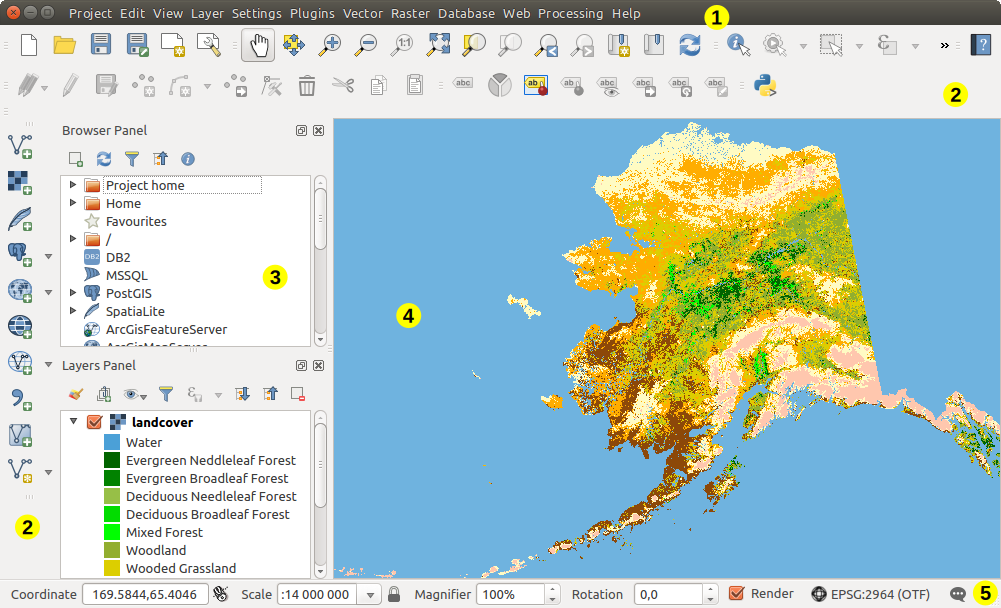
\includegraphics[clip=true, width=12cm]{startup}
    \caption{显示 Alaska 地区示例数据的 QGIS GUI \nixcaption (KDE)} \label{fig:startup}
\end{figure}

\textbf{注意:} 您的窗口装饰(标题栏等)可能因操作系统和窗口管理器的不同而不同。\\

QGIS GUI被划分为六个区域:

\begin{tabular}{p{5cm} p{5cm}}
%\centering
1. 菜单栏  & 4. 地图显示区 \\
2. 工具栏 & 5. 地图预览区 \\
3. 图例显示区 & 6. 状态栏 \\
\end{tabular}

下面各节对QGIS界面这六大部分进行了更加详尽的描述。还有两节介绍了键盘快捷键和上下文帮助。

% \newpage

\subsection{菜单栏}\label{label_menubar}
\index{menus}

菜单栏通过标准的分层菜单向用户提供了各种QGIS功能。下面列出了顶层菜单和一些菜单选项的汇总及其对应的工具栏上的图标和键盘快捷键。 \footnote{键盘快捷键现在可以手动配置(本节中给出快捷键是默认的版本),只需要点击设置菜单项下的自定义快捷键命令}虽然大部分菜单选项都有相应的工具,反之亦然,但是菜单并没有像工具栏一样安排有序。每次进入菜单选项选择复选框后工具栏中包含的所有工具都会被列出。更多关于工具和工具栏的信息详见章节 \ref{label_toolbars}。

\begin{tabbing}
\hspace{5.5cm}\=\hspace{3cm}\=\hspace{3.5cm}\= \kill
\hspace{1cm} 菜单选项 \> 快捷键 \> 参考章节 \> 工具栏\\
\end{tabbing}

\begin{itemize}
\item \mainmenuopt{文件}
\begin{tabbing}
\hspace{4.5cm}\=\hspace{3cm}\=\hspace{3.5cm}\= \kill
\dropmenuopttwo{mActionFileNew}{新建工程}
	\> \keystroke{Ctrl+N}
	\> 参见章 \ref{sec:projects}
	\> \dropmenucheck{文件} \\
\dropmenuopttwo{mActionFileOpen}{打开工程}
	\> \keystroke{Ctrl+O}
	\> 参见章 \ref{sec:projects}
	\> \dropmenucheck{文件} \\
\dropmenuopt{打开最近工程}
	\>
	\> 参见章 \ref{sec:projects} \\
\dropmenuopttwo{mActionFileSave}{保存工程}
	\> \keystroke{Ctrl+S}
	\> 参见章 \ref{sec:projects}
	\> \dropmenucheck{文件} \\
\dropmenuopttwo{mActionFileSaveAs}{工程另存为}
	\> \keystroke{Ctrl+Shift+S}
  \> 参见章 \ref{sec:projects}
	\> \dropmenucheck{文件} \\
\dropmenuopttwo{mActionSaveMapAsImage}{另存为图像}
	\>
	\> 参见章 \ref{sec:output} \\
\dropmenuopttwo{mActionNewComposer}{新建打印设置}
        \> \keystroke{Ctrl+P}
        \> 参见章 \ref{label_printcomposer}
        \> \dropmenucheck{文件} \\
\dropmenuopttwo{mActionComposerManager}{打印设置}
	\>
	\> 参见章 \ref{label_printcomposer}
	\> \dropmenucheck{文件} \\
\dropmenuopt{打印设置}
	\>
	\> 参见章 \ref{label_printcomposer} \\
\dropmenuopttwo{mActionFileExit}{退出}
	\> \keystroke{Ctrl+Q} \\
\end{tabbing}

\item \mainmenuopt{编辑}
\begin{tabbing}
\hspace{4.5cm}\=\hspace{3cm}\=\hspace{3.5cm}\= \kill
\dropmenuopttwo{mActionUndo}{撤销}
        \> \keystroke{Ctrl+Z}
        \> 参见章 \ref{sec:advanced_edit}
        \> \dropmenucheck{高级数字化} \\
\dropmenuopttwo{mActionRedo}{重做}
        \> \keystroke{Ctrl+Shift+Z}
        \> 参见章 \ref{sec:advanced_edit}
        \> \dropmenucheck{高级数字化} \\
\dropmenuopttwo{mActionEditCut}{图元剪切}
	\> \keystroke{Ctrl+X}
	\> 参见章 \ref{sec:edit_existing_layer}
	\> \dropmenucheck{数字化} \\
\dropmenuopttwo{mActionEditCopy}{图元复制}
	\> \keystroke{Ctrl+C}
	\> 参见章 \ref{sec:edit_existing_layer}
	\> \dropmenucheck{数字化} \\
\dropmenuopttwo{mActionEditPaste}{图元粘贴}
	\> \keystroke{Ctrl+V}
	\> 参见章 \ref{sec:edit_existing_layer}
	\> \dropmenucheck{数字化} \\
\dropmenuopttwo{mActionEditPaste}{图元移动}
        \>
        \> 参见章 \ref{sec:edit_existing_layer}
        \> \dropmenucheck{数字化} \\
\dropmenuopttwo{mActionDeleteSelected}{删除选中图元}
        \>
        \> 参见章 \ref{sec:edit_existing_layer}
        \> \dropmenucheck{数字化} \\
\dropmenuopttwo{mActionSimplify}{图元简化}
        \>
        \> 参见章 \ref{sec:advanced_edit}
        \> \dropmenucheck{高级数字化} \\
\dropmenuopttwo{mActionAddRing}{添加环}
        \>
        \> 参见章 \ref{sec:advanced_edit}
        \> \dropmenucheck{高级数字化} \\
\dropmenuopttwo{mActionAddIsland}{添加部分}
        \>
        \> 参见章 \ref{sec:advanced_edit}
        \> \dropmenucheck{高级数字化} \\
\dropmenuopttwo{mActionDeleteRing}{删除环}
        \>
        \> 参见章 \ref{sec:advanced_edit}
        \> \dropmenucheck{高级数字化} \\
\dropmenuopttwo{mActionDeletePart}{删除部分}
        \>
        \> 参见章 \ref{sec:advanced_edit}
        \> \dropmenucheck{高级数字化} \\
\dropmenuopttwo{mActionReshape}{图元调整}
        \>
        \> 参见章 \ref{sec:advanced_edit}
        \> \dropmenucheck{高级数字化} \\
\dropmenuopttwo{mActionSplitFeatures}{图元分割}
        \>
        \> 参见章 \ref{sec:advanced_edit}
        \> \dropmenucheck{高级数字化} \\
\dropmenuopttwo{mActionMergeFeatures}{合并选中图元}
        \>
        \> 参见章 \ref{sec:advanced_edit}
        \> \dropmenucheck{高级数字化} \\
\dropmenuopttwo{mActionNodeTool}{结点工具}
        \>
        \> 参见章 \ref{sec:edit_existing_layer}
        \> \dropmenucheck{数字化} \\
\dropmenuopttwo{mActionRotatePointSymbols}{旋转点状符号}
        \>
        \> 参见章 \ref{sec:advanced_edit}
        \> \dropmenucheck{高级数字化} \\
\end{tabbing}

在对图层激活 \toolbtntwo{mActionToggleEditing}{启动编辑} 工具后,您会在菜单 \mainmenuopt{编辑} 下发现一个捕捉图元的图标,具体取决于图层类型(点,线或面)。\\

\begin{tabbing}
\hspace{4.5cm}\=\hspace{3cm}\=\hspace{3.5cm}\= \kill
\dropmenuopttwo{mActionCapturePoint}{点捕捉}
        \>
        \> 参见章 \ref{sec:edit_existing_layer}
        \> \dropmenucheck{数字化} \\
\dropmenuopttwo{mActionCaptureLine}{线捕捉}
        \>
        \> 参见章 \ref{sec:edit_existing_layer}
        \> \dropmenucheck{数字化} \\
\dropmenuopttwo{mActionCapturePolygon}{多边形捕捉}
        \>
        \> 参见章 \ref{sec:edit_existing_layer}
        \> \dropmenucheck{数字化} \\
\end{tabbing}


\item \mainmenuopt{视图}
\begin{tabbing}
\hspace{4.5cm}\=\hspace{3cm}\=\hspace{3.5cm}\= \kill
\dropmenuopttwo{mActionPan}{地图漫游}
	\>
	\> \> \dropmenucheck{地图导航} \\
\dropmenuopttwo{mActionZoomIn}{地图放大}
	\> \keystroke{Ctrl++}
	\> \> \dropmenucheck{地图导航} \\
\dropmenuopttwo{mActionZoomOut}{地图缩小}
	\> \keystroke{Ctrl+-}
	\> \> \dropmenucheck{地图导航} \\
\dropmenuopttwo{mActionSelect}{图元选择}
	\> 
	\> 参见章 \ref{sec:selection} 
	\> \dropmenucheck{属性} \\
\dropmenuopttwo{mActionDeselectAll}{取消所有选中图元}
        \>
        \> \> \dropmenucheck{属性} \\
\dropmenuopttwo{mActionIdentify}{图元标记}
	\> \keystroke{Ctrl-Alt-I}
	\> \> \dropmenucheck{属性} \\
\dropmenuopttwo{mActionMeasure}{直线量测}
	\> \keystroke{Ctrl-Alt-M}
	\> \> \dropmenucheck{属性} \\
\dropmenuopttwo{mActionMeasureArea}{面积量测}
	\> \keystroke{Ctrl-Alt-J}
	\> \> \dropmenucheck{属性} \\
\dropmenuopttwo{mActionMeasureAngle}{角度量测}
	\>
	\> \> \dropmenucheck{属性} \\
\dropmenuopttwo{mActionOpenTable}{按屏幕缩放}
	\> \keystroke{Ctrl-Alt-F}
	\> \> \dropmenucheck{地图导航} \\
\dropmenuopttwo{mActionZoomToLayer}{按图层缩放}
	\>
	\> \> \dropmenucheck{地图导航} \\
\dropmenuopttwo{mActionZoomToSelected}{按选择区缩放}
	\> \keystroke{Ctrl+J}
	\> \> \dropmenucheck{地图导航} \\
\dropmenuopttwo{mActionZoomLast}{返回最后一次缩放}
	\>
	\> \> \dropmenucheck{地图导航} \\
\dropmenuopttwo{mActionZoomNext}{重做下一次缩放}
	\>
	\> \> \dropmenucheck{地图导航} \\
\mainmenuopt{按实际大小缩放}
	\>
	\> \>  \\
\dropmenuopttwo{mActionMapTips}{地图小技巧}
	\>
	\> \> \dropmenucheck{属性} \\
\dropmenuopttwo{mActionNewBookmark}{新建书签}
	\> \keystroke{Ctrl+B}
	\> 参见章 \ref{sec:bookmarks}
\> \dropmenucheck{属性} \\
\dropmenuopttwo{mActionShowBookmarks}{显示书签}
	\> \keystroke{Ctrl-Alt-B}
	\> 参见章 \ref{sec:bookmarks}
	\> \dropmenucheck{属性} \\
\dropmenuopttwo{mActionDraw}{刷新}
	\> \keystroke{Ctrl+R}
	\> \> \dropmenucheck{地图导航} \\
\mainmenuopt{平铺缩放条}
	\>
	\> 参见章 \ref{sec:tilesets}
	\> \dropmenucheck{平铺缩放条} \\
\mainmenuopt{Live GPS tracking}
	\>
	\> 参见章 \ref{sec:gpstracking}
	\> \dropmenucheck{GPS 信息} \\
\end{tabbing}

\item \mainmenuopt{图层}
\begin{tabbing}
\hspace{5cm}\=\hspace{3cm}\=\hspace{3.5cm}\= \kill
\dropmenuopt{新建}
	\>
	\> 参见章 \ref{sec:create shape}
	\> \dropmenucheck{图层管理} \\
\mainmenuopt{栅格图层计算}
        \>
        \> 参见章 \ref{sec:raster_calc}
        \>  \\
\dropmenuopttwo{mActionAddNonDbLayer}{添加矢量图层}
	\> \keystroke{Ctrl+Shift+V}
	\>
	参见章 \ref{label_workingvector}
	\> \dropmenucheck{图层管理} \\
\dropmenuopttwo{mActionAddRasterLayer}{添加栅格图层}
	\> \keystroke{Ctrl+Shift+R}
	\>
	参见章 \ref{label_raster}
	\> \dropmenucheck{图层管理} \\
\dropmenuopttwo{mActionAddLayer}{添加PostGIS图层}
	\> \keystroke{Ctrl+Shift+D}
	\>
	参见章 \ref{label_postgis}
        \> \dropmenucheck{图层管理} \\
\dropmenuopttwo{mActionAddSpatiaLiteLayer}{添加SpatiaLite图层}
        \> \keystroke{Ctrl+Shift+L}
        \>
        参见章 \ref{label_spatialite}
	\> \dropmenucheck{图层管理} \\
\dropmenuopttwo{mActionAddWmsLayer}{添加WMS图层}
	\> \keystroke{Ctrl+Shift+W}
	\>
	参见章 \ref{sec:ogc-wms}
	\> \dropmenucheck{图层管理} \\
\dropmenuopttwo{mActionOpenTable}{打开属性表}
	\> \>
	\> \dropmenucheck{属性} \\
\dropmenuopttwo{mActionFileSave}{保存修改}
        \> \>
        \> \dropmenucheck{数字化} \\
\dropmenuopttwo{mActionToggleEditing}{启动编辑状态}
	\> \>
	\> \dropmenucheck{数字化} \\
\mainmenuopt{另存为。。。}
	\\
\mainmenuopt{选区另存为矢量图层。。。}
	\> 
	\> See \ref{sec:attribute table}
	\> \\
\dropmenuopttwo{mActionRemoveLayer}{移除图层}
	\> \keystroke{Ctrl+D}
	\>
	\> \dropmenucheck{特性} \\
\mainmenuopt{特性}
	\\
\mainmenuopt{查询。。。}
	\\
\dropmenuopttwo{mActionInOverview}{添加到预览}
	\> \keystroke{Ctrl+Shift+O}
	\>
	\> \dropmenucheck{图层管理} \\
\dropmenuopttwo{mActionAddAllToOverview}{全部添加到预览}
	\>
	\>
	\\
\dropmenuopttwo{mActionRemoveAllFromOverview}{从预览移除全部}
	\>
	\>
	\\
\dropmenuopttwo{mActionHideAllLayers}{隐藏所有图层}
	\> \keystroke{Ctrl+Shift+H}
	\>
	\> \dropmenucheck{图层管理} \\
\dropmenuopttwo{mActionShowAllLayers}{显示所有图层}
	\> \keystroke{Ctrl+Shift+U}
	\>
	\> \dropmenucheck{图层管理} \\
\dropmenuopttwo{labeling}{标注}
	\>
	\>
	\\
\end{tabbing}

\item \mainmenuopt{设置}
\begin{tabbing}
\hspace{5cm}\=\hspace{3cm}\=\hspace{3.5cm}\= \kill
\dropmenuopt{面板}
	\>
	\>
	\\
\dropmenuopt{工具栏}
	\>
	\>
	\\
\mainmenuopt{启动全屏模式}
	\>\keystroke{Ctrl-F}
	\>
	\\
\dropmenuopttwo{mActionProjectProperties}{工程设置}
	\> \keystroke{Ctrl-Alt-P}
	\> 参见章 \ref{sec:projects} \\
\dropmenuopttwo{mActionCustomProjection}{自定义CRS}
        \> \> 参见章 \ref{sec:customprojections} \\
\mainmenuopt{样式管理}
        \> \> \\
\dropmenuopttwo{mActionOptions}{自定义快捷键}
        \> \> \\
\dropmenuopttwo{mActionOptions}{选项}
        \> \> 参见章 \ref{subsec:gui_options} \\
\end{tabbing}

\item \mainmenuopt{插件} - (添加由插件扩展的菜单项。)
\begin{tabbing}
\hspace{5cm}\=\hspace{3cm}\=\hspace{3.5cm}\= \kill
\dropmenuopttwo{mActionShowPluginManager}{插件管理}
	\> \> 参见章 \ref{sec:managing_plugins} \dropmenucheck{插件}
	\\
	\mainmenuopt{Python终端}
        \> \>
        \\
\end{tabbing}

\item \mainmenuopt{帮助}
\begin{tabbing}
\hspace{5cm}\=\hspace{3cm}\=\hspace{3.5cm}\= \kill
\dropmenuopttwo{mActionHelpContents}{帮助上下文}
	\> \keystroke{F1}
	\>
	\> \dropmenucheck{帮助}\\
\dropmenuopttwo{mActionQgisHomePage}{QGIS主页}
	\> \keystroke{Ctrl+H}
	\>
	\\
\dropmenuopttwo{mActionCheckQgisVersion}{查看QGIS版本}
	\\
\dropmenuopttwo{mActionHelpAbout}{关于}
	\\
\end{tabbing}

\end{itemize}

\textbf{注意:} \nix 上面列出的菜单栏项在KDE窗口管理器中都是默认的。在GNOME中没在“设置”菜单项,但在以下这些地方可以找到:

\begin{tabbing}
\dropmenuopttwo{mActionProjectProperties}{工程设置} \hspace{3cm}\=
\dropmenucheck{文件菜单} \\
\dropmenuopttwo{mActionOptions}{选项} \hspace{3cm}\>
\dropmenucheck{编辑}\\
\dropmenuopttwo{mActionOptions}{自定义快捷键} \hspace{3cm}\>
\dropmenucheck{编辑}\\
\mainmenuopt{样式管理} \hspace{3cm}\>
\dropmenucheck{编辑}\\
\dropmenuopttwo{mActionCustomProjection}{自定义CRS}\hspace{3cm}\>
\dropmenucheck{编辑} \\
\dropmenuopt{面板} \hspace{3cm}\>
\dropmenucheck{视图} \\
\dropmenuopt{工具栏}   \hspace{3cm}\>
\dropmenucheck{视图} \\
\mainmenuopt{启动全屏模式} \hspace{3cm}\>
\dropmenucheck{视图} \\
\mainmenuopt{平铺缩放条} \hspace{3cm}\>
\dropmenucheck{视图} \\
\mainmenuopt{GPS实时跟踪} \hspace{3cm}\>
\dropmenucheck{视图} \\
\end{tabbing}

%See Appendix \ref{app_menu} for complete descriptions of the menu items.

\subsection{工具栏}\label{label_toolbars}
\index{toolbars}

工具栏提供了大部分与菜单相同的功能,另外还提供了与地图进行交互访问的工具。每个工具栏项都可弹出帮助,将鼠标停留在工具项上就会显示该工具的简单描述。
每个菜单条都可以据需要而移动。另外,在工具栏点击鼠标右键显示快捷菜单可选择关闭菜单条。

\begin{Tip}
\caption{\textsc{重置工具栏}} \index{layout!toolbars}
如果不小心隐藏所有工具栏,可以选择 \mainmenuopt{设置} \arrow \dropmenuopt{工具栏} 使之再度出现。
\end{Tip}

\subsection{图例显示区}\label{label_legend}
\index{legend}

地图图例区用于设置图层可见性和叠置次序。叠置顺序是指接近说明顶层的图层在较低层的图层之上。每个说明条目的复选框都可用于显示或者隐藏图层。\index{layer!visibility}
在地图图例窗口的图层可以通过增加一个图层组或者接拖拽图层到一个组而对图层进行分组。操作如下,移动鼠标指针到图例窗口,点击右键,选择 \dropmenuopt{添加图层组} ,一个新的文件夹就出现。然后将图层拖到文件夹标志处。那么只需点击一次就可看到该组所有图层。鼠标右键点击图层标志选择 \dropmenuopt{移至最顶级} ,就将图层移出该组。在组右键菜单选择 \dropmenuopt{重命名} 对文件夹重新命名。
鼠标右键菜单目录取决于鼠标停在所加载的图例是栅格还是矢量图层。对于GRASS矢量图层,是不可用的。关于GRASS矢量图层的信息详见章节 \ref{grass_digitising} 。

\begin{itemize}

\item \textbf{栅格图层的右键菜单}
\begin{itemize}
\item \dropmenuopt{按图层边界缩放}
\item \dropmenuopt{按最佳比例缩放(100\%)}
\item \dropmenuopt{显示预览}
\item \dropmenuopt{移除}
\item \dropmenuopt{图层属性}
\item \dropmenuopt{重命名}
\item \dropmenuopt{添加图层组}
\item \dropmenuopt{展开全部}
\item \dropmenuopt{收起全部}
%%\item \dropmenuopt{Show file groups}
\end{itemize}

\item \textbf{矢量图层的右键菜单}
\begin{itemize}
\item \dropmenuopt{按图层边界缩放}
\item \dropmenuopt{显示预览}
\item \dropmenuopt{移除}
\item \dropmenuopt{打开属性表}
\item \dropmenuopt{开始编辑(对 GRASS 图层不可用)}
\item \dropmenuopt{另存为}
\item \dropmenuopt{选区另存为}
\item \dropmenuopt{查询}
\item \dropmenuopt{图层特性}
%% \item \dropmenuopt{Make to toplevel item}
\item \dropmenuopt{重命名}
\item \dropmenuopt{添加图层组}
\item \dropmenuopt{展开全部}
\item \dropmenuopt{收起全部}
%%\item \dropmenuopt{Show file groups}
\end{itemize}

\item \textbf{矢量图层的右键菜单}
\begin{itemize}
\item \dropmenuopt{移除}
\item \dropmenuopt{重命名}
\item \dropmenuopt{添加图层组}
\item \dropmenuopt{展开全部}
\item \dropmenuopt{收起全部}
%%\item \dropmenuopt{Show file groups}
\end{itemize}

\end{itemize}

如果几个矢量数据源有相同的矢量类型和属性,那么它们的符号可被分组。也就是说如果一个数据源的符号改变,则其他几个也作出改变。在图例窗口中打开右键菜单选择 \dropmenuopt{添加图层组},出现图层文件组。就可以将文件从一个文件组拖拽到另一个文件组。这样就使符号分组。注意QGIS只能拖拽两个具有相同符号体系(相同的矢量几何体类型和相同的属性)的图层。

用鼠标左键选择图层的同时按住 \keystroke{CTRL}-键,就可以选择多个图层或图层组。然后您可以将选中图层全部加入一个新的图层组。


同样地,您也可以先按住 \keystroke{CTRL}-键选择几个图层,然后按 \keystroke{CTRL-D}-来一次性地删除多个图层或图层组。这样选中的图层或图层组就会从图层列表中移除。

%% isn't included in Titan anymore, except for an "toggle overview"
%Each legend entry can show the following mini icons:
%
%\includegraphics[width=0.7cm]{pyramid} This is a raster
%that has pyramids built for it to improve rendering efficiency (see
%Section \ref{raster_pyramids}).\\
%\includegraphics[width=0.7cm]{no_pyramid} This is a
%raster that has no pyramid layers (参见章 \ref{raster_pyramids}).\\
%\includegraphics[width=0.7cm]{inoverview} This layer is
%shown in the overview map area as well as in the main map window.\\
%\includegraphics[width=0.7cm]{editable} This is a vector
%layer that is currently enabled for editing.\\

\subsection{地图显示区}\label{label_mapview}
\index{map!view}

这是QGIS的“业务端点”——地图在这个区域显示!在这个窗口显示的地图将取决于所选择加载的图层(后续章节将会介绍如何加载图层)。地图视图可以平移和缩放(变换地图焦点到另一个地区)。其他各种操作可以如上述工具栏所描述的在地图上执行。地图视图和图例彼此紧密联系——图例区的改变会在视图中反映出来。

\begin{Tip}\caption{\textsc{使用鼠标滚轮缩放窗口}}\index{zoom!mouse wheel}
您可以使用鼠标滚轮缩放地图。将鼠标光标放到地图区域内向前滚动滚轮(远离您)放大地图,向后滚动(对着您)缩小地图。光标的位置就是缩放的中心。您可以通过 \mainmenuopt{设置} \arrow \dropmenuopt{选项} 下的菜单 \tab{地图工具} 来自定义鼠标滚轮缩放。
\end{Tip}

\begin{Tip}\caption{\textsc{使用方向键和空格键来进行地图平移}}\index{pan!arrow keys}
您可以使用方向键平移地图。把鼠标光标放在地图区域,敲击右方向键则地图向东平移,左方向键向西平移,上方向键向北平移,下方向键向南平移。您也可以用空格键平移地图:只需要按住空格键的同时移动鼠标即可。
\end{Tip}

\subsection{预览区地图}\label{label_mapoverview}
\index{map!overview}

地图全览面版提供了加载图层的完整范围的视图。可在 \mainmenuopt{设置} \arrow \dropmenuopt{面板} 菜单下选择地图概观。该视图是一个显示当前地图范围的矩形框。这使您可以快速确定当前正在查看的地图区。请注意即使在地图概观的图层已经设置标签,标签也不会在地图概观中显示出来。

您可以通过在图例窗口中右键点击图层,并选中 \checkbox{显示预览} 将一个单独的图层增加到地图概观中。您还可以通过工具栏中的概观工具来添加图层或移除概观中的所有图层。

如果在地图概观中单击并拖动显示当前范围的红色矩形框,地图的主要视图将会作出相应的更新。

\subsection{状态栏}\label{label_statusbar}

当鼠标指针在整个地图视图上移动时,状态栏显示出您在地图坐标系统中的当前位置(例如米或者十进制度数)。在状态栏显示坐标的左边是一个小按钮,用于显示坐标位置和显示平移与缩放地图范围之间的切换。

状态栏的进度条显示了每个图层添加到地图视图的渲染进度。在某些情况下,如在栅格图层统计数据收集,进度栏将被用于显示冗长的操作状态。

如果一个新的插件或者插件更新可用时,你会在状态栏看到消息。在状态栏右侧是一个小的复选框用于暂时阻止图层被渲染到地图视图(参见后面的章 \ref{subsec:redraw_events})。在状态栏的最右侧是一个投影图标。点击它打开当前项目的投影属性。

\begin{Tip}\caption{\textsc{计算您的地图区正确的缩放比例}}\index{scale!calculate}
当启动QGIS时,经纬度是默认的单位,它告诉QGIS图层的任何坐标都是用经纬度表示的。为了得到正确的缩放值,您可以在 \mainmenuopt{设置} \arrow \dropmenuopt{工程属性} 菜单下的 \tab{通用} 标签页中手动改成“米”,也可以在右下角状态栏处点击图标 \toolbtntwo{mIconProjectionDisabled}{projector} 。这样就可以根据工程投影的设定来确定地图单位,比如‘+units=m’
\end{Tip}

\subsection{键盘快捷键}\label{shortcuts}
\index{Keyboard shortcuts}

QGIS为许多功能提供了默认的快捷键,参见后面的 \ref{label_menubar} 。除此之外,菜单选项 \mainmenuopt{设置} \arrow
\dropmenuopt{自定义快捷键} 允许改变默认快捷键并为QGIS功能添加新的快捷键。

\begin{figure}[ht]
   \centering
   \includegraphics[clip=true, width=8cm]{shortcuts}
   \caption{自定义快捷键 \nixcaption (KDE)} \label{fig:shortcuts}
\end{figure}

自定义非常简单,只需从列表中选择一个功能并点击 \button{更改} , \button{取消快捷键} 或者 \button{设为默认} 。一旦用户建立了自己的配置,就可以将其存储为XML文件并加载到另一个QGIS装置。

\subsection{帮助上下文}\label{context_help}
\index{Context help}

当您需要特定主题的帮助时,可以通过在大部分对话框都可获得的Help按钮进入内容帮助——请注意第三方插件可以指向专门的网页。

\section{渲染}\label{subsec:redraw_events}\index{rendering}

默认情况下,每当地图画布必须被刷新的时候QGIS就会渲染所有可视图层。引发刷新地图画布的事件包括:

\begin{itemize}
\item 添加图层
\item 平移或缩放
\item QGIS窗口大小调整
\item 改变图层或图层集的可见度
\end{itemize}

QGIS允许用户用许多方式控制渲染过程。

\subsection{缩放相关的渲染}\index{rendering!scale dependent}
\label{label_scaledepend}

缩放相关的渲染可以指定每个图层可见的最小和最大比例。在图例显示区双击图层打开 \dialog{图层属性} 对话框可以设置缩放相关的渲染。在 \tab{通用} 标签页中,设置最小和最大比例值然后点击复选框 \checkbox{使用缩放相关的渲染} 即可。

用户可以通过缩放想要使用的水平并注意QGIS状态栏的缩放值来确定缩放数值。 \index{scale}

\subsection{地图渲染控制}\label{label_controlmap}

地图渲染可通过以下方式控制:

\minisec{a) 暂停渲染}\index{rendering!suspending}
\label{label_suspendrender}

在状态栏右下角点击 \checkbox{渲染} 复选框可暂停渲染。当 \checkbox{渲染} 复选框未选中时,QGIS都不会响应 \ref{subsec:redraw_events} 中所描述的任何事件来重绘画布。可能需要暂停渲染的例子有:

\begin{itemize}

\item 添加许多图层并更改其绘制的优先级
\item 绘图之前添加一个或者多个大图层并设置缩放比例
\item 绘图之前添加一个或者多个大图层并缩放至特定视图
\item 上述情形的任意组合
\end{itemize}

选中 \checkbox{渲染} 复选框可以渲染并且即使刷新地图画布。

\minisec{b) 设置图层添加的选项}\label{label_settinglayer}
\index{rendering!options}\index{layers!initial visibility}

用户可以设置一个选项,使之总是可以装载新的图层而不用绘图。这意味着该图层将被添加到地图中,但是其在图例窗口中的可见性复选框将默认为未选中。选择菜单选项 \mainmenuopt{设置}  \arrow \dropmenuopt{选项} 并点击 \tab{绘制 \& SVG} 标签页。取消选中 \checkbox{默认不显示新添加图层} 复选框之后,添加到地图的所有新图层都将默认关闭(不可见)。

%\minisec{Stopping Rendering}\index{rendering!halting}
%\label{label_stoprender}
%
%To stop the map drawing, press the ESC key. This will halt the refresh of
%the map canvas and leave the map partially drawn. It may take a bit of time
%between pressing ESC and the time the map drawing is halted.
%
%\textbf{NOTE}: It is currently not possible to stop rendering - this was disabled
%in qt4 port because of User Interface (UI) problems and crashes.

\minisec{c) 渲染时更新地图显示}
\label{label_updatemap}\index{rendering!update during drawing}

您可以在绘制图元时设置更新地图显示。默认情况下,QGIS不显示图层的任何要素直到全部图层被渲染。选择菜单 \mainmenuopt{设置} \arrow \dropmenuopt{选项} 项并点击 \tab{渲染 \& SVG} 标签,可对数据储存处读取的要素显示进行更新。将特征值设置为一个适当的值可在渲染过程中显示更新。将值设置为0将禁用绘图更新(这是默认值)。设置值过低会导致在读取要素过程中地图画布不断更新时较差性能。建议设置初始值为500。

\minisec{d) 影响渲染质量}
\label{label_renderquality}\index{rendering!quality}

有三个选项可影响地图的渲染质量。选择菜单选项 \mainmenuopt{设置} \arrow \dropmenuopt{选项},点击 \tab{渲染 \& SVG} 标签页,选中或取消选中以下复选框。

\begin{itemize}
\item \checkbox{牺牲部分绘制速度以提高线条抗锯齿}
\item \checkbox{修复多边形填充错误}
\end{itemize}

\section{量度}\label{sec:measure}\index{measure}

测量只能在投影坐标系中进行(例如 UTM)。如果加载的是一个地理坐标系(经/纬度)下的地图,那么线或区域的测量结果将是错误的。为了解决这个问题用户需要设置一个合适的地图坐标系统(参见节 \ref{label_projections} )。两种测量模块还使用了数字化模块捕捉设置。这对于在矢量图层沿着线或者区测量是有用的。

要选择测量工具,请单击 \includegraphics[width=0.7cm]{mActionMeasure} ,然后选择需要的工具。

\subsection{长度、面积和角度量度}
\index{measure:line length}
\index{measure:areas}
\index{measure:angles}

\includegraphics[width=0.7cm]{mActionMeasure}
QGIS也可以依据定义的椭圆体测量给定点之间的实地距离。若要进行设置,选择菜单选项 \mainmenuopt{设置} \arrow \dropmenuopt{选项},然后点击 \tab{地图工具} 标签并选择适当的参考椭球体。也可在此处定义一个橡皮条颜色和首选测量单位(米或者英尺)。然后该工具就允许用户点击地图上的点。每段长度以及总长度都会显示在测量窗口。点击鼠标右键就可停止测量。 \\

\includegraphics[width=0.7cm]{mActionMeasureArea} 面积也可以量度。在测量窗口显示出累计的面积大小。此外,测量工具将捕捉到当前选中图层,该图层提供捕捉容限值设置(参见节 \ref{snapping_tolerance} )。所以,如果想测量精确的线要素或面要素首先设置其捕捉容限值,然后选中图层。那么当使用测量工具时,每个鼠标点击(在设置公差范围内)都将捕捉此图层。 \\

\includegraphics[width=0.7cm]{mActionMeasureAngle}
选中测量角度工具也可测量角度。光标变成十字形的。点击绘制您希望测量的的角度的第一段,然后移动光标绘制要求的角度。测量结果会显示在一个弹出的对话框。

\begin{figure}[ht]
\centering
   \subfloat[长度量度] {\label{subfig:measure_line}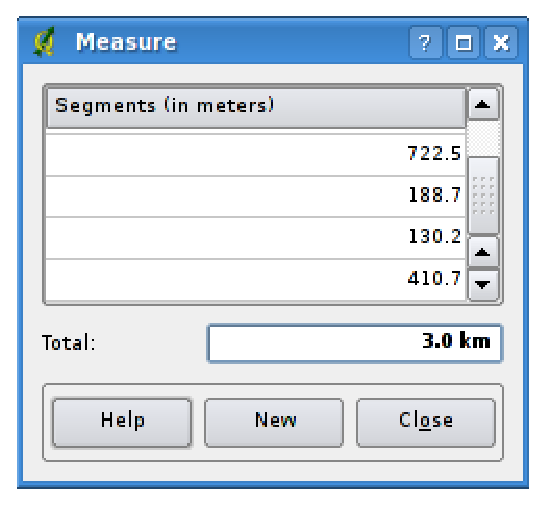
\includegraphics[clip=true, width=0.3\textwidth]{measure_line}}
     \hspace{0.33cm}
   \subfloat[面积量度]{\label{subfig:measure_area}
\includegraphics[clip=true, width=0.3\textwidth]{measure_area}}
     \hspace{0.33cm}
   \subfloat[角度量度]{\label{subfig:measure_angle}\includegraphics[clip=true, width=0.3\textwidth]{measure_angle}}
   \caption{实践中的量度工具 \nixcaption} \label{fig:measure}
\end{figure}

\subsection{选择和取消选择图元}\label{sec:selection}

QGIS 工具条上可以有好几种工具来选中地图显示区内的图元。要单选或多选图元,只需要单击 \includegraphics[width=0.7cm]{mActionSelect} ,然后悬着工具:

\begin{description}
\item \radiobuttonon{选择图元}
\item \radiobuttonoff{矩形选择}
\item \radiobuttonoff{多边形选择}
\item \radiobuttonoff{自由形状选择}
\item \radiobuttonoff{半径选择}
\end{description} 

单击 \includegraphics[width=0.7cm]{mActionDeselectAll} 可以取消所有图元的选择.

\section{工程}\label{sec:projects}\index{projects}

一个 QGIS 项目被组织成为一个工程。QGIS一次只能工作于某一个工程。工程属性或者是分工程设置,或者作为新工程的默认值进行设置(参见节 \ref{subsec:gui_options})。通过菜单 \mainmenuopt{文件} \arrow \dropmenuopt{mActionFileSave}{保存工程} 或者 \mainmenuopt{文件} \arrow \dropmenuopt{mActionFileSave}{工程另存为} 可以将您的工作空间保存为工程文件。

通过 \mainmenuopt{文件} \arrow \dropmenuopt{mActionFileSave}{打开工程} 或者  \mainmenuopt{文件} \arrow \dropmenuopt{mActionFileSave}{打开最近工程} 可以在 QGIS 会话中加载保存的工程文件。

如果您希望清空当前会话并重新开始,选择 \mainmenuopt{文件} \arrow \dropmenuopttwo{mActionFileNew}{新建工程} 。在打开或者最后一次保存一个工程后,如果工程文件已经被修改,那么以上各菜单选项都会提示您保存已有工程文件。

工程文件中保存的信息包括:

\begin{itemize}
\item 已添加的图层
\item 包括图例在内的图层属性
\item 地图的投影
\item 最后的视图范围
\end{itemize}

工程文件被保存为XML格式,因此可以独立于QGIS来修改该文件,只要你知道你在干什么。该文件的格式与早期版本相比的话已经有了较大变化。老版本的工程文件可能不能正常工作。为了记住这个问题,你需要在 \mainmenuopt{设置} \arrow \dropmenuopt{选项} 下的 \tab{通用} 标签页中选中:

\checkbox{需要时提示保存工程文件} \\
\checkbox{打开一个旧版本工程文件时提出警告}

\minisec{工程特性}
在 \nix{\mainmenuopt{文件} \arrow \dropmenuopt{工程特性}} 或者 \win{\mainmenuopt{设置} \arrow
\dropmenuopt{工程特性}} 弹出的特性窗口中,你可以设置特定的工程选项,包括:

\begin{itemize}
\item 在 \tab{通用} 标签页中可以设置工程标题、选择区、背景颜色、图层单位、准确度和保存路径到图层等选项。并且此处也可以设置拓扑编辑和图层级别的节点捕捉选项。
\item \tab{参考坐标系统} 坐标系统标签页可以设置工程的参考坐标系,并且在显示其它坐标系统的矢量文件时可以动态转换投影。
\item 第三个 \tab{可查询图层} 标签页中你可以设置(或禁用)相应到属性查询工具的图层,见( \ref{subsec:gui_options} 部分可以启用多图层的属性查询。)
\end{itemize}

\section{输出}\label{sec:output}
\index{output!save as image!print composer!quick print}

有许多方法可以从你的QGIS会话中生成输出文件。 \ref{sec:projects} 部分中已经讨论了一种方法:保存为工程文件。

此处提供了一些产生其它输出文件的例子:

\begin{itemize}
\item 菜单项 \dropmenuopttwo{mActionSaveMapAsImage}{保存为图像} 会打开一个文件对话框,你可以在其中选择文件名、文件路径和文件类型(PNG或JPG)。相同文件夹下以PNGW或JPGW后缀保存的引用参照文件(world file)对该图像进行地理索引。
\item 菜单项 \dropmenuopttwo{mActionFilePrint}{打印设置} 会打开一个对话框,你可以设置输出样式并打印当前的地图显示区,参见 \ref{label_printcomposer} 。
\item \toolbtntwo{quick_print}{快速打印} 插件使得可以通过最少的设置来进行打印,参见章 \ref{quickprint} 。
\end{itemize}

\section{GUI选项}\label{subsec:gui_options}

\includegraphics[width=0.7cm,clip=true]{mActionOptions} 可以在 \dialog{选项} 对话框中设置一些QGIS的选项。选择菜单项 \mainmenuopt{设置} \arrow
\dropmenuopttwo{mActionOptions}{选项} 。你可以自定义选项设置的标签页如下:

\minisec{通用标签页}

\begin{itemize}
\item \checkbox{需要时提示保存工程文件}
\item \checkbox{打开一个旧版本工程文件时提出警告}
\item 改变选择项颜色和背景色
\item 改变图标主题(在默认(default)、传统(classic)、gis和newgis中切换)
\item \checkbox{图例中的图层名大写}
\item \checkbox{图例中显示分类属性}
\item \checkbox{图例中创建栅格图标}
\item \checkbox{启动时隐藏飞溅屏幕} 即 splash screen
\item \checkbox{查询窗口结果以Dock窗口的形式显示(QGIS需要重启)}
\item \checkbox{属性表窗口以Dock窗口的形式显示}
\item \checkbox{扩展模式中双击和选择来添加PostGIS图层}
\item \checkbox{添加图层至选择组}
\item 属性表行为(在显示所有图元(默认)、显示选择的图元二者中进行选择,图元显示在当前的地图区域)
\end{itemize}

\minisec{绘制 \& SVG标签页}

\begin{itemize}
\item \checkbox{默认显示新添加的图层}
\item 设置更新显示前绘制的图元数量
\item \checkbox{尽量使用渲染缓存来加速地图绘制}
\item \checkbox{忽略其它效果以使线段反锯齿}
\item \checkbox{修复填充多边形错误的问题}
\item \checkbox{渲染时使用新的图标}
\item 添加或删除搜索可缩放矢量图形(SVG)文件的路径
\end{itemize}

此外,在菜单项 \mainmenuopt{设置} \arrow \dropmenuopttwo{mActionOptions}{项目特性} 下的标签页 \tab{通用} 中可定义存储SVG文件的绝对或相对路径。

\minisec{地图工具标签页}

\begin{itemize}
\item 模式设置通过标识工具确定哪一图层将被显示出来。通过设置 \usertext{上下} 或 \usertext{上下,但到第一层为止} ,而不是 \usertext{当前图层},所有图层上图元的属性(参见 \ref{sec:projects} 的项目属性部分来设置哪些图层可查询)都可以用查询工具显示出来。
\item \checkbox{查询单个图元时打开图元窗口}
\item 为识别和显示地图提示设置搜索半径作为地图宽度的百分比
\item 设置距离计算的椭球体
\item 设置测量工具橡皮圈颜色
\item \radiobuttonon{设置默认的量测单位(米或英尺)}
\item \radiobuttonon{设置默认的角度单位(度,弧度或百分度)}
\item 设置鼠标滚轮行为(缩放,缩放并重定位,缩放鼠标光标处,无变化)
\item 设置鼠标滚轮缩放因子
\end{itemize}

\minisec{叠置标签页}

\begin{itemize}
\item 为标签设置位置选择算法(包括中心点法,chain, popmusic tabu chain,popmusic tabut和popmusic chain)
\end{itemize}

\minisec{数字化标签页}

\begin{itemize}
\item 设置橡皮圈线的颜色和宽度
\item 设置默认捕捉模式(顶点捕捉,线段捕捉,顶点和线段捕捉)
\item 设置地图单位或像素的默认捕捉容限值
\item 设置地图单位或像素的顶点编辑搜索半径
\item \checkbox{仅对选中图元显示标记}
\item 设置顶点标记样式(十字形(默认),半透明圆或者无)和顶点标记大小
\item \checkbox{创建图元之后不弹出属性窗口}
\end{itemize}

\minisec{参考坐标系(CRS)标签页}

\begin{itemize}
\item \radiobuttonoff{弹出选择参考坐标系(CRS)}
\item \radiobuttonoff{使用项目默认的参考坐标系(CRS)}
\item \radiobuttonon{使用全局默认的参考坐标系(CRS)}
\item 选择全局默认的参考坐标系(CRS)
\end{itemize}

\minisec{用户区域设置(Locale)标签页}

\begin{itemize}
\item \checkbox{使用自定义的区域设置覆盖系统设置}
\item 活动的系统区域设置信息
\end{itemize}

\minisec{代理标签页}

\begin{itemize}
\item \checkbox{设置网络连接的等待时间(毫秒)}
\item \checkbox{使用代理进行网络连接} 并设置主机名、端口、用户名和口令密码。
\item 根据您的需要选择 \dropmenuopt{代理类型}
 \begin{itemize}
  \item \dropmenuopt{默认代理类型}: 使用应用程序使用的代理。
  \item \dropmenuopt{Socks5 代理}: 支持所有类型连接的通用代理。其支持TCP、UDP、端口绑定(接入连接)和代理验证。
  \item \dropmenuopt{Http 代理}: 使用“CONNECT”命令进行设置,仅支持接出的TCP连接,同时支持代理验证。
  \item \dropmenuopt{Http 缓冲代理}: 使用常规的HTTP命令进行设置,仅在发送HTTP请求时有效。
  \item \dropmenuopt{Ftp缓冲代理}: 使用FTP代理服务器连接,仅在发送FTP请求时有效。
 \end{itemize}
\end{itemize}

通过单击 \button{添加} 按钮向代理设置(参见图 \ref{fig:proxy-settings} )下的文本框中添加URL地址可以排除该地址。双击进入可编辑的URL字段区域,然后输入您想要排除的URL值,可以不通过代理访问该地址。同样地,按钮 \button{移除} 会删除新建的规则。

如果您还想了解更多的关于不同代理设置的信息,请自行查阅 \url{http://doc.trolltech.com/4.5/qnetworkproxy.html#ProxyType-enum} 下的QT库使用说明文档。

\begin{figure}[ht]
   \centering
   \includegraphics[clip=true, width=14cm]{proxy-settings}
   \caption{\qg 里的代理设置 \nixcaption}
   \label{fig:proxy-settings}
\end{figure}

\begin{Tip} \caption{\textsc{使用代理}}
使用代理有时候会比较麻烦,需要不断地尝试以上的代理类型以适合您的具体状况。
\end{Tip}

您可以根据需求修改选项。有些改变可能要求重启QGIS才能生效。

\begin{itemize}
\item \nix{设置文件以文本文件格式保存在:\$HOME/.config/QuantumGIS/qgis.conf}
\item \osx{设置文件保存在: \$HOME/Library/Preferences/org.qgis.qgis.plist}
\item \win{设置信息保存在注册表项:}
\begin{verbatim}
\\HKEY\CURRENT\USER\Software\QuantumGIS\qgis
\end{verbatim}
\end{itemize}

\section{注释工具}\label{sec:annotations}
\index{annotations}
\index{text annotation|\see{annotations}}

使用属性工具条上的 \includegraphics[width=0.7cm,clip=true]{mActionTextAnnotation}文本注释工具可以在QGIS的显示区域内以格式化文本的形式显示一个注释气球。选择注释工具然后在地图显示区域内单击即可。

\begin{figure}[ht]
   \centering
   \includegraphics[clip=true, width=12cm]{annotation}
   \caption{文本注释对话框 \nixcaption}
   \label{fig:annotation}
\end{figure}

双击文档打开一个多选项对话框。包括进入规定文本格式的文本编辑器和其他设置项。例如,是将注释放置在一个地图位置(通过点要素显示)上还是一个屏幕位置(与地图无关)上。此注释可在地图中移动(拖拽地图标记)或者只移动气球。

注释移动工具 \includegraphics[width=0.7cm,clip=true]{mActionAnnotation}可以在地图上移动注释文本。

\subsection{窗体注释}\index{annotations}
\index{form annotation|\see{annotations}}

此外,用户也可以创建一个自己的注释表格。表格注释工具对于在自定义设计器的表格中显示一个矢量图层的属性是很有用的(参见图 \ref{fig:custom-annotations})。其类似于识别工具的设计形式,但是在注释项中显示。详情参见QGIS博客: \url{http://blog.qgis.org/node/143}

\begin{figure}[ht]
   \centering
   \includegraphics[clip=true, width=10cm]{custom_annotation}
   \caption{自定义QT Designer的注释窗体 \nixcaption}
   \label{fig:custom-annotations}
\end{figure}

\newpage

\section{空间位置书签}\label{sec:bookmarks}
\index{bookmarks}
\index{spatial bookmarks|\see{bookmarks}}

空间位置书签使得您可以 ``bookmark'' 一个地理位置并可以在以后重新访问之。

\subsection{创建书签}
要创建书签:
\begin{enumerate}
\item 缩放并定位至目标区域。
\item 选择 \mainmenuopt{视图} \arrow \dropmenuopt{新建标签} 命令或按 \keystroke{Ctrl-B} 键。
\item 为新书签输入一个有意义的名字(最多255字符。
\item 单击 \button{确定} 按钮以添加该书签,或 \button{取消} 按钮以取消添加并退出。
\end{enumerate}

注:您可以添加多个同名的书签。

\subsection{使用书签}
要使用或者管理书签,请选择 \mainmenuopt{视图} \arrow \dropmenuopt{显示书签} 命令。 \dialog{地理位置书签} 对话框允许您缩放至书签位置,或者删除书签。

书签的名字和坐标不允许编辑。

\subsection{缩放至书签位置}
在 \dialog{地理位置书签} 对话框中单击选中目标书签位置,然后单击 \button{缩放至} 按钮。

双击某书签也可以直接访问之。

\subsection{删除书签}
在 \dialog{地理位置书签} 对话框中单击选中目标书签位置,然后单击 \button{删除} 按钮可以删除该书签位置。选择 \button{是} 确认删除, \button{否}取消删除。

\section{动态GPS追踪}\label{sec:gpstracking}

要激活QGIS的动态GPS追踪功能,您需要选择 \mainmenuopt{视图} \arrow \dropmenuopt{动态GPS追踪} 菜单项。地图区的左边会弹出一个新的Dock窗口。

GPS追踪窗口里有4中显示试图(参见图 \ref{fig:gpstrack_live} 和图 \ref{fig:gpstrack_options} )。

\begin{description}
 \item[(a)] \includegraphics[width=0.5cm,clip=true]{mActionToggleEditing} GPS位置坐标视图,用于手工输入顶点和图元
 \item[(b)] \includegraphics[width=0.5cm,clip=true]{gpstrack_barchart} GPS卫星连接信号强度视图
 \item[(c)] \includegraphics[width=0.5cm,clip=true]{gpstrack_polarchart} GPS卫星视图,用于显示卫星数量和位置
 \item[(d)] \includegraphics[width=0.5cm,clip=true]{mActionOptions} GPS选项设置视图(参见 \ref{fig:gpstrack_options}).
\end{description}

插入GPS接收机之后(需要操作系统的支持),单击 \button{连接} 按钮可以将GPS连接到QGIS。之后单击 \button{断开连接} 会断开GPS接收机与您电脑之间的连接。GNU/Linux系统的QGIS集成了gpsd支持可以连接大部分的GPS接收机,因此需要您正确地配置了gpsd以连接QGIS和GPS。

[ 重要提示 ]: 要想在地图区追踪GPS位置,需要创建一个新的图层并设置其为可编辑状态。

\begin{figure}[ht]
\centering
   \subfloat[位置坐标视图] {\label{subfig:gpstrack_main}\includegraphics[clip=true, width=0.3\textwidth]{gpstrack_main}}
     \hspace{0.33cm}
   \subfloat[GPS信号视图]{\label{subfig:gpstrack_stren}\includegraphics[clip=true, width=0.3\textwidth]{gpstrack_stren}}
     \hspace{0.33cm}
   \subfloat[GPS卫星视图]{\label{subfig:gpstrack_polar}\includegraphics[clip=true, width=0.3\textwidth]{gpstrack_polar}}
\caption{动态GPS追踪 \nixcaption} \label{fig:gpstrack_live}
\end{figure}

\begin{figure}[ht]
   \centering
   \includegraphics[clip=true, width=4cm]{gpstrack_options}
   \caption{GPS追踪选项设置窗口 \nixcaption}
   \label{fig:gpstrack_options}
\end{figure}

\subsection{位置坐标视图}
\includegraphics[width=0.5cm,clip=true]{mActionToggleEditing} 如果您的GPS能接收到信号,你会发现GPS点的位置以纬度、经度和高程的格式给出,参见图 \ref{subfig:gpstrack_main}

\subsection{GPS信号视图}
\includegraphics[width=0.5cm,clip=true]{gpstrack_barchart} 您可以在这里查看GPS接受的信号的强度(参见图 \ref{subfig:gpstrack_stren} )。

\subsection{GPS卫星视图}
\includegraphics[width=0.5cm,clip=true]{gpstrack_polarchart} 如果您想要知道GPS连接的卫星在天空中的位置的话,您需要切换到卫星视图(参见图 \ref{subfig:gpstrack_polar}。您好可以查看信号卫星的ID编号。

\subsection{GPS选项设置}
\includegraphics[width=0.5cm,clip=true]{mActionOptions} 为了避免连接问题,您可以切换 \radiobuttonon{自动检测} 到 \radiobuttonon{使用自定义路径和端口} ,然后选择GPS接收机连接到的路径和端口。单击 \button{连接} 会重新建立到GPS接收机的连接。

使用 \slider{GPS指针大小} 可以调整地图上位置指针的大小。选中 \radiobuttonon{自动添加顶点} ,对GPS的追踪结果会自动记录到当前激活的矢量图层(可编辑状态)。

使用GPS地图记录器(recenter)可以设定记录的坐标点发生修改或超出地图范围时,地图的更新方式。

追踪颜色和线宽决定绘制追踪路径的颜色和线宽。

如果您想要手动设置某个图元,你需要返回 \includegraphics[width=0.5cm,clip=true]{mActionToggleEditing} ''位置坐标视图'' 并单击 \button{添加图元} 按钮。同理,如果您没有激活 ''自动添加顶点`` 功能,你只能返回该处并单击 \button{添加顶点} 手动添加顶点。

\FloatBarrier

% vim:autoindent:set textwidth=78:

\section{Working with Vector Data}\label{label_workingvector}
\index{vector layers|(}

QGIS supports vector data in a number of formats, including those
supported by the OGR library data provider plugin, such as ESRI shapefiles,
\index{shapefiles}
\index{ESRI!shapefiles}
\index{SHP files}
MapInfo MIF (interchange format)
\index{MIF files}
\index{MapInfo!MIF files}
and MapInfo TAB (native format).
\index{TAB files}
\index{MapInfo!TAB files}
QGIS also supports PostGIS
\index{PostGIS}
\index{PostgreSQL!PostGIS}
layers in a PostgreSQL database using the PostgreSQL data provider plugin.
Support for
additional data types (eg. delimited text) is provided by additional data provider plugins.
\index{delimited text}

This section describes how to work with two common formats:
ESRI shapefiles and PostGIS layers. Many of the
features available in QGIS work the same regardless of the vector data source.
This is by design and includes the identify, select, labeling and attributes
functions.

Working with GRASS vector data is described in Section \ref{sec:grass}.

\subsection{ESRI Shapefiles}
\index{vector layers!ESRI shapefiles}
\index{shapefiles}
\index{ESRI!shapefiles}
\index{SHP files}

ESRI Shapefile support is provided by a library of functions known as 
the OGR Simple Feature Library (\url{http://www.gdal.org/ogr})\index{OGR}. See Appendix
\ref{appdx_ogr} for a list of all supported formats in OGR.

A shapefile actually consists of a minimum of three
files:\index{shapefile!format}

\begin{itemize}
\item \filename{.shp} file containing the feature geometries.
\item \filename{.dbf} file containing the attributes in dBase format.
\item \filename{.shx} index file.
\end{itemize}

Ideally it comes with another file with a \filename{.prj} suffix, that contains
the projection information for the shapefile.

There can be more files belonging to a shapefile dataset.
To have a closer look at this we recommend the technical specification for the shapefile format,
that can be found at \url{http://www.esri.com/library/whitepapers/pdfs/shapefile.pdf}\index{shapefile!specification}.

\subsubsection{Loading a Shapefile}\label{sec:load_shapefile}
%FIXME {\includegraphics[width=0.7cm]{addshapefile}} 
To load a shapefile, start
QGIS and click on the 
%FIXME \toolbtntwo{addshapefile}{Add a vector layer}
toolbar button\index{shapefile!loading} or simply type \keystroke{V}. This same tool can be used to
load any of the formats supported by the OGR library.

Clicking on the tool brings up a standard open file dialog (see Figure
\ref{fig:openshapefile}) which allows you to navigate the file system and load
a shapefile or other supported data source. 
The selection box \selectstring{Files of type}{\ldots} allows you to preselect some OGR supported file formats.

You can also select the Encoding type for the shapefile if desired.

%\begin{figure}[ht]
%   \begin{center}
%   \caption{Open an OGR Supported Vector Layer Dialog}\label{fig:openshapefile}\smallskip
%   \includegraphics[clip=true, width=14cm]{shapefileopendialog}
%\end{center} 
%\end{figure}

Selecting a shapefile from the list and clicking \button{Open} loads it into QGIS. Figure
\ref{fig:loadedshapefile} shows QGIS after loading the \filename{alaska.shp} file.

%\begin{figure}[ht]
%   \begin{center}
%   \caption{QGIS with Shapefile of Alaska loaded}\label{fig:loadedshapefile}\smallskip
%   \includegraphics[clip=true, width=17cm]{shapefileloaded09}
%\end{center} 
%\end{figure}

\begin{Tip}\caption{\textsc{Layer Colors}}
\qgistip{When you add a layer to the map, it is assigned a random color. When
adding more than one layer at a time, different colors are assigned to each. }
\end{Tip}

Once loaded, you can zoom around the shapefile using the map navigation tools.
To change the symbology of a layer, open the \dialog{Layer Properties} dialog by double
clicking on the layer name or by right-clicking on the name in the legend and
choosing \dropmenuopt{Properties} from the popup menu. See
Section \ref{sec:symbology} for more information on setting symbology of
vector layers.
  
\subsubsection{Improving Performance}

To improve the performance of drawing a shapefile, you can create a spatial
index. A \index{spatial index!shapefiles} spatial index will improve the 
speed of both zooming and panning. Spatial indexes used by QGIS have a 
\filename{.qix} extension.

Use these steps to create the index:

\begin{itemize}
\item Load a shapefile.
\item Open the \dialog{Layer Properties} dialog by double-clicking on the
shapefile name in the legend or by right-clicking and choosing
\dropmenuopt{Properties} from the popup menu.
\item In the tab \tab{General} click the \button{Create} button on the Spatial
Index section.
\end{itemize}

\subsubsection{Loading a MapInfo Layer}
\index{vector layers!MapInfo}

To load a MapInfo layer, click on the 
%FIXME \toolbtntwo{addshapefile}{Add a vector layer}
toolbar bar button or type \keystroke{V}, change the file type filter to
\selectstring{Files of Type}{[OGR] MapInfo (*.mif
*.tab *.MIF *.TAB)} and select the layer you want to load.

\subsubsection{Loading an ArcInfo Coverage}
\index{vector layers!ArcInfo Coverage}

Loading an ArcInfo coverage is done using the same method as with a
shapefiles and MapInfo layers. Click on the 
%FIXME \toolbtntwo{addshapefile}{Add a vector layer}
toolbar button or type \keystroke{V} to open the 
\dialog{Open on OGR Supported Vector Layer} 
dialog and change the file type filter to
\selectstring{Files of Type}{All files (*.*)}. Navigate to the coverage directory and select one
of the following files (if present in your coverage):

\begin{itemize}
\item \filename{.lab} - to load a label layer (polygon labels or standing points).
\item \filename{.cnt} - to load a polygon centroid layer 
\item \filename{.arc} - to load an arc (line) layer.
\item \filename{.pal} - to load a polygon layer.
\end{itemize}

\subsection{PostGIS Layers}
\index{vector layers!PostGIS|see{PostGIS}}
\index{PostGIS!layers}
\label{label_postgis} 

PostGIS layers are stored in a PostgreSQL database. The advantages of PostGIS
are the spatial indexing, filtering and query capability. Using PostGIS,
vector functions such as select and identify work more accurately than with
OGR layers in QGIS.

To use PostGIS layers you must:\index{PostgreSQL!loading layers}

\begin{itemize}
\item Create a stored connection in QGIS to the PostgreSQL database (if one is
not already defined).\index{PostgreSQL!connection}
\item Connect to the database.
\item Select the layer to add to the map.
\item Optionally provide a SQL \usertext{where}
clause to define which features
to load from the layer.
\item Load the layer.
\end{itemize}

\subsubsection{Creating a stored
Connection}\index{PostgreSQL!connection}\label{sec:postgis_stored}

\includegraphics[width=0.7cm]{mActionAddLayer} The first time
you use a PostGIS data source, you must create a connection to the PostgreSQL
database that contains the data. Begin by clicking on the
\toolbtntwo{mActionAddLayer}{Add a PostGIS Layer} toolbar button, selecting the
\dropmenuopttwo{mActionAddLayer}{Add a PostGIS Layer...} option from the \mainmenuopt{Layer} menu or typing
\keystroke{D}. 
The \dialog{Add PostGIS Table(s)} dialog will
be displayed. To access the connection manager\index{PostgreSQL!connection
manager}, click on the \button{New} button to display the \dialog{Create a New
PostGIS Connection} dialog. The parameters required for a connection are shown
in table \ref{tab:postgis_connection_parms}.

\begin{table}[ht]\index{PostgreSQL!connection parameters}
\centering
\caption{PostGIS Connection
Parameters}\label{tab:postgis_connection_parms}\medskip
 \begin{tabular}{|l|p{5in}|}
\hline Name & A name for this connection. Can be the same as \textsl{Database}.
\\
\hline Host \index{PostgreSQL!host}
& Name of the database host. This must be a resolvable host name the same as
would be used to open a telnet connection or ping the host. \\
\hline Database \index{PostgreSQL!database} & Name of the database.  \\
\hline Port \index{PostgreSQL!port}& Port number the PostgreSQL database
server listens on. The default port is 5432.\\
\hline Username \index{PostgreSQL!username}& User name used to login to the
database. \\
\hline Password \index{PostgreSQL!password}& Password used with
\textsl{Username} to connect to the database.\\
\hline
\end{tabular}
\end{table}

Once the parameters have been filled in, you can test the connection by
clicking on the \button{Test
Connection} button\index{PostgreSQL!connection!testing}. To save the password
with the connection information, check the \checkbox{Save Password} option.

\begin{Tip}\caption{\textsc{QGIS User Settings and
Security}}\index{settings}\index{security}
\qgistip{Your customized settings for QGIS are stored based on the operating
system. \nix, the settings are stored in your home directory in
\filename{.qt/qgisrc}. \win, the settings are stored in the registry. Depending on
your computing environment, storing passwords in your QGIS settings may be a
security risk.
}
\end{Tip}

\subsubsection{Loading a PostGIS Layer}\index{PostgreSQL!loading layers}

\includegraphics[width=0.7cm]{mActionAddLayer} Once you have one or more
connections defined, you can load layers from the PostgreSQL database. Of
course this requires having data in PostgreSQL. See Section
\ref{sec:loading_postgis_data} for a discussion on importing data into the
database. 

To load a layer from PostGIS, perform the following steps:

\begin{itemize}
\item If the \dialog{Add PostGIS Table(s)} dialog is not already open, click on the
\toolbtntwo{mActionAddLayer}{Add a PostGIS Layer} toolbar button.
\item Choose the connection from the drop-down list and click \button{Connect}.
\item Find the layer you wish to add in the list of available layers.
\item Select it by clicking on it. You can select multiple layers by holding
down the \keystroke{shift} key while clicking. See Section \ref{sec:query_builder} for
information on using the PostgreSQL Query Builder to further define the layer.
\item Click on the \button{Add} button to add the layer to the map.
\end{itemize}

\begin{Tip}\caption{\textsc{PostGIS Layers}}
\qgistip{Normally a PostGIS layer is defined by an entry in the
geometry\_columns table. From version \OLD % should be 0.9.0 
on, QGIS can load layers that do not have
an entry in the geometry\_columns table. This includes both tables and views.
Defining a spatial view provides a powerful means to visualize your data. Refer
to your PostgreSQL manual for information on creating views.}
\end{Tip}

\subsubsection{Some details about PostgreSQL
layers}\label{sec:postgis_details}
\index{PostgreSQL!layer details}

This section contains some details on how QGIS accesses PostgreSQL
layers. Most of the time QGIS should simply provide you with a list of
database tables that can be loaded, and load them on request. However,
if you have trouble loading a PostgreSQL table into QGIS, the information
below may help you understand any QGIS messages and give you direction on
changing the PostgreSQL table or view definition to allow QGIS to load it.

QGIS requires that PostgreSQL layers contain a column that can be
used as a unique key for the layer. For tables this usually means
that the table needs a primary key, or have a column with a unique
constraint on it. QGIS additionally requires that this column be of
type int4 (an integer of size 4 bytes). If a table lacks these items,
the oid column will be used instead. Performance will be improved if the
column is indexed (note that primary keys are automatically indexed in
PostgreSQL). 

If the PostgreSQL layer is a view the same requirements exist, but
views don't have primary keys or columns with unique constraints on
them. In this case QGIS will try to find a column in the view that is
derived from a table column that is suitable. If one cannot be found,
QGIS will not load the layer. If this occurs, the solution is to alter
the view so that it does include a suitable column (a type of int4
and either a primary key or with a unique constraint, preferably indexed).

\subsubsection{Importing Data into PostgreSQL}\label{sec:loading_postgis_data}
\index{PostGIS!SPIT!importing data}

\minisec{shp2pgsql}
Data can be imported into PostgreSQL using a number of methods. PostGIS
includes a utility called \filename{shp2pgsql} that can be used to import shapefiles into
a PostGIS enabled database. For example, to import a shapefile named
\filename{lakes.shp}
into a PostgreSQL database named \usertext{gis\_data}, use the following command:

\begin{verbatim} 
  shp2pgsql -s 2964 lakes.shp lakes_new | psql gis_data
\end{verbatim}

This creates a new layer named \usertext{lakes\_new} in the
\usertext{gis\_data} database. The
new layer will have a spatial reference identifier (SRID) of 2964. See Section 
\ref{label_projections} for more information on spatial reference systems and
projections.
\begin{Tip}
\caption{\textsc{Exporting datasets from PostGIS}\index{PostGIS!Exporting}}
\qgistip{Like the import-tool \filename{shp2pgsql} there is also a tool to export
PostGIS-datasets into shapefiles: \filename{pgsql2shp}. This is shipped within your
PostGIS distribution.} 
\end{Tip}

\minisec{SPIT Plugin}
\includegraphics[width=0.7cm]{spit} QGIS comes with a
plugin named 
SPIT (Shapefile to PostGIS Import Tool)\index{PostGIS!SPIT}.
SPIT can be used to load multiple shapefiles at one time and includes support
for schemas. To use SPIT, open the Plugin Manager from the \mainmenuopt{Plugins}
menu, check the box next to the \checkbox{SPIT plugin} and click \button{OK}. The SPIT
icon will be added to the plugin toolbar\index{PostGIS!SPIT!loading}. 

To import a shapefile, click on the \toolbtntwo{spit}{SPIT} tool in the 
toolbar to open the 
\dialog{SPIT - Shapefile to PostGIS Import Tool} dialog.
You can add one or more files to the queue by clicking on the \button{Add}
button. To process the files, click on the \button{Import} button. The progress of the
import as well as any errors/warnings will be displayed as each shapefile is
processed.  

\begin{Tip}\caption{\textsc{Importing Shapefiles Containing
PostgreSQL Reserved Words}}\index{PostGIS!SPIT!reserved words}
\qgistip{If a shapefile is added to the queue containing fields that are
reserved words in the PostgreSQL database a dialog will popup showing the
status
of each field. You can edit the field names\index{PostGIS!SPIT!editing field names}
prior to import and change any that are reserved words (or change any other
field names as desired). Attempting to
import a shapefile with reserved words as field names will likely fail.}
\end{Tip} 

\minisec{ogr2ogr}
Beside \filename{shp2pgsql} and \filename{SPIT} there is another tool for feeding
geodata in PostGIS: \filename{ogr2ogr}. This is part of your GDAL installation.
To import a shapefile into PostGIS, do the following:
\begin{verbatim}
  ogr2ogr -f "PostgreSQL" PG:"dbname=postgis host=myhost.de user=postgres \
  password=topsecret" alaska.shp
\end{verbatim}

This will import the shapefile \filename{alaska.shp} into the PostGIS-database
\usertext{postgis}
using the user \usertext{postgres} with the password \usertext{topsecret} on host
\server{myhost.de}.

Note that OGR must be built with PostgreSQL to support PostGIS.
You can see this by typing
\begin{verbatim}
ogrinfo --formats | grep -i post
\end{verbatim}

\subsubsection{Improving Performance}\label{label_improve}

Retrieving features from a PostgreSQL database can be time consuming,
especially over a network. You can improve the drawing performance of
PostgreSQL layers by ensuring that a \index{PostGIS!spatial index} spatial
index
exists on each layer in the database. PostGIS supports creation of a
\index{PostGIS!spatial index!GiST} GiST
(Generalized Search Tree) index to speed up spatial searches of the data.

The syntax for creating a GiST\footnote{GiST index information is taken from the PostGIS
documentation available at \url{http://postgis.refractions.net}}
index is:

\begin{verbatim}
    CREATE INDEX [indexname] ON [tablename] 
      USING GIST ( [geometryfield] GIST_GEOMETRY_OPS );
\end{verbatim}

Note that for large tables, creating the index can take a long time. Once the
index is created, you should perform a \usertext{VACUUM ANALYZE}. See the
PostGIS documentation \cite{PostGISweb} for more information.

The following is an example of creating a GiST index:
\begin{verbatim}
gsherman@madison:~/current$ psql gis_data
Welcome to psql 8.3.0, the PostgreSQL interactive terminal.

Type:  \copyright for distribution terms
        \h for help with SQL commands
        \? for help with psql commands
        \g or terminate with semicolon to execute query
        \q to quit

gis_data=# CREATE INDEX sidx_alaska_lakes ON alaska_lakes
gis_data-# USING GIST (the_geom GIST_GEOMETRY_OPS);
CREATE INDEX
gis_data=# VACUUM ANALYZE alaska_lakes;
VACUUM
gis_data=# \q
gsherman@madison:~/current$
\end{verbatim}

\subsection{The Vector Properties Dialog}\label{sec:vectorprops}
\index{vector layers!properties dialog}

The \dialog{Layer Properties} dialog for a vector layer 
provides information about the layer, symbology
settings and labeling options. If your vector layer has been loaded from a
PostgreSQL / PostGIS datastore, you can also alter the underlying SQL for the
layer - either by hand editing the SQL on the \tab{General} tab or by
invoking the \dialog{Query Builder} dialog on the \tab{General} tab. 
To access the
\dialog{Layer Properties} dialog, double-click on a layer in the legend or right-click on the
layer and select \dropmenuopt{Properties} from the popup menu.

\subsubsection{Symbology Tab}\label{sec:symbology}
\index{vector layers!symbology}

QGIS supports a number of symbology renderers to control how
vector features are displayed. Currently the following renderers
are available:

\begin{description}
    \item[Single symbol] - a single style is applied to every
    object in the layer.\index{vector layers!renderers!single symbol}
    \item[Graduated symbol] - objects within the layer are
    displayed with different symbols classified by the values of a
    particular field.\index{vector layers!renderers!graduated symbol}
    \item[Continuous colour] - objects within the layer are
    displayed with a spread of colours classified by the numerical
    values within a specified field.\index{vector layers!renderers!continuous
color}
    \item[Unique value] - objects are classified by the unique
    values within a specified field with each value having a
    different symbol.\index{vector layers!renderers!unique value}
\end{description}

To change the symbology for a layer, simply double click on its legend 
entry and the vector \dialog{Layer Properties} dialog will be 
shown.\index{symbology!changing}.

%\begin{figure}[H]
%   \begin{center}
%   \caption{Vector Layer Properties
%Dialog}\label{fig:vector_symbology}\smallskip
%   \includegraphics[clip=true, width=12cm]{vectorLayerSymbology09} 
%\end{center}  
%\end{figure}

Since \usertext{version v0.9} there is a function to use image files stored on 
your computer as fill pattern for vector layers.

\minisec{Vector transparency} \label{sec:vect_transparency} \index{vector layers!transparency}
QGIS \CURRENT allows to set a transparency for every vector layer. This can be done with
the slider right below the legend type (see fig. \ref{fig:vector_symbology}).
This is very useful for overlaying several vector layers.

\subsubsection{General Tab}
The \tab{General} tab is essentially like that of the raster dialog. It allows you
to change the display name, set scale dependent rendering options, create a spatial 
index of the vector file (only for OGR supported formats and PostGIS) and view or
change the projection.

The \button{Query Builder} button allows you to create a subset of the features 
in the layer - but this button currently only is available when you open the 
attribute table and select the \button{Advanced ...} button.

\subsubsection{Metadata Tab}

The \tab{Metadata} tab contains information about the layer, including specifics
about the type and location, number of features, feature type, and the editing
capabilities. The \guiheading{Layer Spatial Reference System} section, providing projection information, and the \guiheading{Attribute field info} section,
listing fields and their data types, are displayed 
on this tab. This is a quick way to get information about the layer.

\subsubsection{Labels Tab}

The \tab{Labels} tab allows you to enable labeling features and control a number of
options related to placement, style and buffering.

We will illustrate this by labelling the lakes shapefile of the
\filename{qgis\_example\_dataset}:

\begin{enumerate}
\item Load the shapefiles \filename{alaska.shp} and \filename{lakes.shp} in QGIS.
\item Zoom in a bit to your favorite area with some lake.
\item Make the \filename{lakes} layer active.
\item Open the \dialog{Layer Properties} dialog.
\item Click on the \tab{Labels} tab.
\item Check the \checkbox{Display labels} checkbox to enable labeling.
\item Choose the field to label with. 
  We'll use \selectstring{Field containing labels}{NAMES}.
\item Enter a default for lakes that have no name. The default label will be
  used each time QGIS encounters a lake with no value in the \guilabel{NAMES} field.
\item Click \button{Apply}.
\end{enumerate} 

Now we have labels. How do they look? They are probably too big and poorly
placed in relation to the marker symbol for the lakes.

Click on the \tab{Font Style} tab and use the \button{Font} and \button{Color}
buttons to set the font and color.

To change the position of the font relative to the feature:

\begin{enumerate} 
\item Click on the \tab{Font Alignment} tab.
\item Change the placement by selecting one of the radio buttons
in the \classname{Placement} group. To fix our labels, choose the
\radiobuttonon{Right} radio button.
\item Click \button{Apply} to see your changes without closing the dialog.
\end{enumerate} 

Things are looking better, but the labels are still too close to the marker. To
fix this we can use the options on the \tab{Position} tab. Here we can add
offsets for the X and Y directions. Adding an X offset of 5 will move our
labels off the marker and make them more readable. Of course if your marker
symbol or font is larger, more of an offset will be required.

The last adjustment we'll make is to \tab{buffer} the labels. This just means
putting a backdrop around them to make them stand out better. To buffer the
lakes labels:

\begin{enumerate}
\item Click the \tab{Buffer} tab.
\item Click the \checkbox{Buffer Labels?} checkbox to enable buffering.
\item Choose a size for the buffer using the spin box.
\item Choose a color by clicking on \button{Colour} and choosing your
  favorite from the color selector.
\item Click \button{Apply} to see if you like the changes.
\end{enumerate} 

If you aren't happy with the results, tweak the settings and then test again
by clicking \button{Apply}.

A buffer of 2 points seems to give a good result.
Notice you can also specify the buffer size in map units if that works out
better for you.

The remaining tabs on the \tab{Label} tab allow you control the appearance of the
labels using attributes stored in the layer. The \tab{Data} tabs allow you to
set all the parameters for the labels using fields in the layer.

\subsubsection{Actions Tab}\index{actions}\label{label_actions}

QGIS provides the ability to perform an action based on the attributes of a
feature. This can be used to perform any number of actions, for example,
running a program with arguments built from the attributes of a feature or
passing parameters to a web reporting tool.

Actions are useful when you frequently want to run an external application or
view a web page based on one or more values in your vector layer. An example
is performing a search based on an attribute value. This concept is used in 
the following discussion.

\minisec{Defining Actions}\index{actions!defining}

Attribute actions are defined from the vector \dialog{Layer Properties} dialog. To
define an action, open the vector \dialog{Layer Properties} dialog and click on the
\tab{Actions} tab. Provide a descriptive name for the action. The action
itself must contain the name of the application that will be executed when the
action is invoked. You can add one or more attribute field values as arguments
to the application. When the action is invoked any set of characters that
start with a \% followed by the name of a field will be replaced by the value of
that field. The special characters \%\% \index{\%\%}will be replaced by the value
of the field that was selected from the identify results or attribute table (see
Using Actions below).  Double quote marks can be used to group text into a
single argument to the program, script or command. Double quotes will be
ignored if preceded by a backslash.

Two example actions are shown below:\index{actions!examples}

\begin{itemize}
  \item \usertext{konqueror http://www.google.com/search?q=\%nam}
  \item \usertext{konqueror http://www.google.com/search?q=\%\%}
\end{itemize}


In the first example, the web browser konqueror is invoked and passed a URL to
open. The URL performs a Google search on the value of the \usertext{nam} field
from our vector layer. Note that the application or script called by the
action must be in the path or you must provided the full path. To be sure, we could
rewrite the first example as: \usertext{/opt/kde3/bin/konqueror
http://www.google.com/search?q=\%nam}. This will ensure that the konqueror
application will be executed when the action is invoked.

The second example uses the \%\% notation which does not rely on a particular
field for its value. When the action is invoked, the \%\% will be replaced by
the value of the selected field in the identify results or attribute table.

\minisec{Using Actions}\index{actions!using}\label{label_usingactions}
Actions can be invoked from either the \dialog{Identify Results} dialog or an
 \dialog{Attribute Table} dialog. 
(Recall that these dialogs can be opened by clicking
\toolbtntwo{mActionOpenTable}{Identify Features}
or
\toolbtntwo{mActionOpenTable}{Open Table}.)
To invoke an action, 
right click on the
record and choose the action from the popup menu. Actions are listed in the popup
menu by the name you assigned when defining the actions. Click on the action you
wish to invoke.

If you are invoking an action that uses the \%\% notation, right-click on the
field value in the \dialog{Identify Results} dialog or the
\dialog{Attribute Table} dialog that you wish to pass to the application or script.

Here is another example that pulls data out of a vector layer and inserts them
into a file using bash and the \usertext{echo} command (so it will only work
\nix or perhaps \osx). The layer in question has fields for a species name
\usertext{taxon\_name}, latitude \usertext{lat} and longitude
\usertext{long}. I would like to be able to
make a spatial selection of a localities and export these field values to a
text file for the selected record (shown in yellow in the QGIS map area). Here is
the action to achieve this:

\begin{verbatim}
  bash -c "echo \"%taxon_name %lat %long\" >> /tmp/species_localities.txt"
\end{verbatim} 

After selecting a few localities and running the action on each one, opening
the output file will show something like this:

\begin{verbatim}
  Acacia mearnsii -34.0800000000 150.0800000000
  Acacia mearnsii -34.9000000000 150.1200000000
  Acacia mearnsii -35.2200000000 149.9300000000
  Acacia mearnsii -32.2700000000 150.4100000000
\end{verbatim} 

As an exercise we create an action that does a Google search on the 
\filename{lakes} layer. First we need to determine the URL needed to perform a search on a
keyword. This is easily done by just going to Google and doing a simple
search, then grabbing the URL from the address bar in your browser. From this
little effort we see that the format is: \url{http://google.com/search?q=qgis},
where \usertext{qgis} is the search term. Armed with this information, we can
proceed:

\begin{itemize}
\item Make sure the \filename{lakes} layer is loaded.
\item Open the \dialog{Layer Properties} dialog by double-clicking on the layer in the
  legend or right-click and choose \dropmenuopt{Properties} from the popup menu.
\item Click on the \tab{Actions} tab.
\item Enter a name for the action, for example \usertext{Google Search}.
\item For the action, we need to provide the name of the external program to
  run. In this case, we can use Firefox. If the program is not in
  your path, you need to provide the full path.
\item Following the name of the external application, add the URL used for
  doing a Google search, up to but not included the search term:
  \url{http://google.com/search?q=}
\item The text in the \guilabel{Action} field should now look like this:\\
  \usertext{firefox \url{http://google.com/search?q=}}
\item Click on the drop-down box containing the field names for the
  \usertext{lakes} layer. It's located just to the right of the
  \button{Insert Field} button.
\item From the drop-down box, select \selectstring{}{NAMES} and click \button{Insert Field}.
\item Your action text now looks like this:\\ \usertext{firefox
  \url{http://google.com/search?q=\%NAMES}}
\end{itemize}
 
This completes the action and it is ready to use. The final text of the action
should look like this:

\begin{center}
\usertext{firefox \url{http://google.com/search?q=\%NAMES}}
\end{center}

We can now use the action. Close the \dialog{Layer Properties} dialog and zoom in to an area
of interest. Make sure the \filename{lakes} layer is active and identify a
lake. In the result box you'll now see that our action is visible:

%\begin{figure}[H]
%   \begin{center}
%   \caption{Select feature and choose action}\label{fig:identify_action}\smallskip
%   \includegraphics[clip=true, width=8cm]{identify_action} 
%\end{center}  
%\end{figure}

When we click on the action, it brings up Firefox and navigates to the URL
\url{http://www.google.com/search?q=Tustumena}. It is also possible to add further 
attribute fields to the action. Therefore you can add a ``+'' to the end of the action 
text, select another field and click on \button{Insert Field}. In this example there 
is just no other field available that would make sense to search for.

You can define multiple actions for a layer and each will show up in the
\dialog{Identify Results} dialog. You can also invoke actions from the attribute table
by selecting a row and right-clicking, then choosing the action from the popup
menu.

You can think of all kinds of uses for actions. For example, if you have a point layer
containing locations of images or photos along with a file name, you could
create an action to launch a viewer to display the image. You could also use
actions to launch web-based reports for an attribute field or combination of
fields, specifying them in the same way we did in our Google search example.

\subsection{Editing}\index{editing}

QGIS supports basic capabilities for editing spatial data.  Before reading any
further you should note that at this stage editing support is still preliminary.
Before performing any edits, always make a backup of the dataset you are about
to edit. 

\textbf{Note} - the procedure for editing GRASS layers is different - see
Section \ref{grass_digitising} for details.

\subsubsection{Setting the Snap Tolerance}

Before we can edit vertices, we need to set the snapping tolerance. This is the 
distance QGIS uses to \usertext{search} for the polygon and vertex you are trying to
edit when you click on the map. If you aren't within the snap tolerance,
QGIS won't find and select the vertex for editing. Tolerance is set in map
units so you may find you need to experiment to get it set right. If you
specify too big of a tolerance, QGIS may snap to the wrong vertex,
especially if you are dealing with a large number of vertices in close
proximity. Set it too small and it won't find anything and it will pop up an
annoying warning to that effect. 

To set the snap tolerance, choose \dropmenuopttwo{mActionOptions}{Project Properties} from the
\mainmenuopt{Settings} menu and click on the \tab{General} tab.  Remember the
tolerance is in map units. For our little digitizing project, the units
are in decimal degrees.  Your results may vary, but something on the order
of 0.05 to 0.1 should be fine. 

\subsubsection{Editing an Existing Layer}
\index{vector layers!editing}
\index{editing!an existing layer}
\label{sec:edit_existing_layer}

By default, QGIS loads layers read-only: This is a safeguard
to avoid accidentally editing a layer if there is a slip of the mouse.
However, you can choose to edit any layer as long as the data provider supports it,
and the underlying data source is writable (i.e. its files are not read-only).

Layer editing is most versatile when used on PostgreSQL/PostGIS data sources. 

\begin{Tip}[ht]\caption{\textsc{Data Integrity}}
\qgistip{Please consider backing up your data source
before you start editing, and also at regular intervals during editing. QGIS is 
still at a pre-version 1.0 stage, and so may not be able to protect your data in all 
situations.
}
\end{Tip}

\index{Allow Editing}
All editing sessions start by choosing the \dropmenuopttwo{mActionToggleEditing}{Allow editing} option.
This can be found in the context menu after right clicking on the legend
entry for that layer.
Alternately, you can use the \index{Toggle Editing}
\toolbtntwo{mActionToggleEditing}{Toggle editing} button from the toolbar to start or stop the editing mode.\index{editing!icons}

\begin{Tip}[ht]\caption{\textsc{Editing a Map is Different to Editing an Attribute Table}}
\qgistip{In this version of QGIS, the \button{Start editing}/\button{Stop editing}
couplet on the map view acts separately to the \button{Start Editing}/\button{Stop Editing}
couplet on the attribute table.
}
\end{Tip}

\begin{Tip}[ht]\caption{\textsc{Save Regularly}}
\qgistip{Remember to toggle \toolbtntwo{mActionToggleEditing}{Allow editing} off regularly.  This allows you to save your changes thus far,
and also confirms that your data source can accept all
your changes.
}
\end{Tip}

\begin{Tip}[ht]\caption{\textsc{Concurrent Edits}}
\qgistip{This version of QGIS does not track if somebody else is editing a feature at the same time
as you.  The last writer wins.
}
\end{Tip}

Once the layer is in edit mode, markers will appear at the
vertices.

\begin{Tip}[ht]\caption{\textsc{Zoom in Before Editing}}
\qgistip{Before editing a layer, you should
zoom in to your area of interest. This 
avoids waiting while all the vertex markers are rendered across the entire layer.
}
\end{Tip}

\begin{Tip}[ht]\caption{\textsc{Vertex Markers}}
\qgistip{This version of QGIS does not allow you to change the vertex markers used.
}
\end{Tip}

You can perform the following editing functions:

\begin{itemize}
\item Add Features: \toolbtntwo{mActionCapturePoint}{point},
  \toolbtntwo{mActionCaptureLine}{line} and
  \toolbtntwo{mActionCapturePolygon}{polygone}
\item \toolbtntwo{mActionMoveFeature}{Move Selected Features}
\item \toolbtntwo{mActionSplitFeatures}{Split Selected Features}
\item \toolbtntwo{mActionDeleteSelected}{Delete Selected Features}
\item \toolbtntwo{mActionAddVertex}{Add Vertex of a Feature}
\item \toolbtntwo{mActionDeleteVertex}{Delete Vertex of a Feature}
\item \toolbtntwo{mActionMoveVertex}{Move Vertex of a Feature}
\item \toolbtntwo{mActionAddRing}{Add Ring}
\item \toolbtntwo{mActionAddIsland}{Add Island}
\item \toolbtntwo{mActionEditCut}{Cut Selected Features}
\item \toolbtntwo{mActionEditCopy}{Copy Selected Features}
\item \toolbtntwo{mActionEditPaste}{Paste Selected Features}
\end{itemize}

\minisec{Adding Features}
\index{vector layers!adding!feature}

Before you start adding features, use the \toolbtntwo{mActionPan}{pan}
and \toolbtntwo{mActionZoomIn}{zoom-in}/\toolbtntwo{mActionZoomOut}{zoom-out} tools to first navigate to the area of interest.

Then you can use the \toolbtntwo{mActionCapturePoint}{Capture point},
\toolbtntwo{mActionCaptureLine}{Capture line} or
\toolbtntwo{mActionCapturePolygon}{Capture polygone} icons on the toolbar to put the QGIS cursor
into digitizing mode.

For each feature, you first digitize the geometry, then enter its attributes.

To digitize the geometry, left-click on the map area to create the
first point of your new feature.

For lines and polygons, keep on left-clicking for each additional
point you wish to capture.  When you have finished adding points,
right-click anywhere on the map area to confirm you have finished entering
the geometry of that feature.

The attribute window will appear, allowing you to enter the information for the new feature.
Figure \ref{fig:vector_digitising} shows setting attributes for a fictitious
new river in Alaska.

%\begin{figure}[ht]
%   \begin{center}
%   \caption{Vector Digitizing Attributes Capture
%Dialog}\label{fig:vector_digitising}\smallskip
%   \includegraphics[clip=true, width=16cm]{digitising_attributes09}
%\end{center}  
%\end{figure}

\begin{Tip}[ht]\caption{\textsc{Attribute Value Types}}
\qgistip{In the current version of QGIS, the attributes
dialog box does not check that the data entered matches the type expected (e.g. numeric 
vs. text). Make sure of this before pressing \button{OK}, otherwise you may find the error
will be caught later when you try to save your changes.
}
\end{Tip}

% These features will be added later
%
%\minisec{Move Selected Feature}
%\index{vector layers!move!feature}
%
%%% INPUT IS MISSING
%
%\minisec{Split Selected Feature}
%\index{vector layers!split!feature}
%
%%%% INPUT IS MISSING
%

\minisec{Editing Vertices of a Feature}
\index{vector layers!editing!vertex}

For both PostgreSQL/PostGIS and shapefile-based layers, the vertices of features can be edited. 

Vertices can be directly edited, that is, you don't
have to choose which feature to edit before you can change
its geometry.
In some cases, several features may share the same vertex
and so the following rules apply when the mouse is pressed
down near map features:

\begin{itemize}
\item \textbf{Lines}    - The nearest line to the mouse position
                          is used as the target feature.
                          Then (for moving and deleting a vertex)
                          the nearest vertex
                          on that line is the editing target.

\item \textbf{Polygons} - If the mouse is inside a polygon, then it is
                          the target feature; otherwise the nearest polygon
                          is used.
                          Then (for moving and deleting a vertex)
                          the nearest vertex
                          on that polygon is the editing target.
\end{itemize}

You will need to set the property
\mainmenuopt{Settings}>\dropmenuopttwo{mActionOptions}{Project
Properties}>\dropmenuopt{General}>\dropmenuopt{Snapping Tolerance}
to a number greater than zero.  Otherwise QGIS will not be able to tell which feature is being edited.


\minisec{Adding Vertices of a Feature}
\index{vector layers!adding!vertex}

You can add new vertices to a feature by using the
\toolbtntwo{mActionAddVertex}{Add Vertex} icon
on the toolbar.

Note, it doesn't make sense to add more vertices to a Point feature!

In this version of QGIS, vertices can only be added to an \textit{existing} line
segment of a line feature.  If you want to extend a line beyond its end,
you will need to move the terminating vertex first, then add a new vertex where
the terminus used to be.

\minisec{Moving Vertices of a Feature}
\index{vector layers!moving!vertex}

You can move vertices using the \toolbtntwo{mActionMoveVertex}{Move Vertex} icon
on the toolbar.

\minisec{Deleting Vertices of a Feature}
\index{vector layers!deleting!vertex}

You can delete vertices by using the \toolbtntwo{mActionDeleteVertex}{Delete Vertex} icon
on the toolbar.

Note, it doesn't make sense to delete the vertex of a Point feature!
Delete the whole feature instead.

Similarly, a one-vertex line or a two-vertex polygon is also
fairly useless and will lead to unpredictable results elsewhere
in QGIS, so don't do that.

\textbf{Warning:} A vertex is identified for deletion as
soon as you click the mouse near an eligible
feature.  To undo, you will need to toggle
Editing off and then discard your changes.
(Of course this will mean that other unsaved changes will be lost, too.)

\minisec{Add Ring}
\index{vector layers!add!ring}
\textbf{New since v0.9}

You can create ring polygons using the \toolbtntwo{mActionAddRing}{Add Ring}
icon in the toolbar. This means inside an existing area it is
possible to digitize further polygons, that will occur as a 'whole', so only 
the area in between the boundaries of the outer and inner polygons remain as 
a ring polygon. 

\minisec{Add Island}
\index{vector layers!add!island}
\textbf{New since v0.9}

You can \toolbtntwo{mActionAddIsland}{add island} polygons to a selected multipolygon. 
The new island polygone 
has to be digitized outside the selected multipolygon. 

% FIXME: In versions > 0.9.0 tries to convert a selected normal polygone to a
% multipolygone, if you try to use the "add island" funtionality. 
% (not yet implemented)

\minisec{Cutting, Copying and Pasting Features}
\index{vector layers!cut!feature}
\index{vector layers!copy!feature}
\index{vector layers!paste!feature}
\index{editing!cutting features}
\index{editing!copying features}
\index{editing!pasting features}

Selected features can be cut, copied and pasted between layers in the
same QGIS project, as long as destination layers are set to 
\toolbtntwo{mActionToggleEditing}{Toggle editing} beforehand.

Features can also be pasted to external applications as text:  That is,
the features are represented in CSV format with the geometry data appearing 
in the OGC Well-Known Text (WKT) format.

However in this version of QGIS, text features from outside QGIS cannot 
be pasted to a layer within QGIS.

When would the copy and paste function come in handy? Well, it turns out that 
you can edit more than one layer at a time and copy/paste features between 
layers. Why would we want to do this?  Say we need to do some work on a new 
layer but only need one or two lakes, not the 5,000 on our \filename{big\_lakes} 
layer. We can create a new layer and use copy/paste to plop the needed lakes 
into it. 

As an example we are copying some lakes to a new layer:

\begin{enumerate}
\item Load the layer you want to copy from (source layer)
\item Load or create the layer you want to copy to (target layer) 
\item Start editing for both layers 
\item Make the source layer active by clicking on it in the legend 
\item Use the \toolbtntwo{mActionSelect}{Select} tool to select the feature(s) on the source layer
\item Click on the \toolbtntwo{mActionEditCopy}{Copy Features} tool
\item Make the destination layer active by clicking on it in the legend 
\item Click on the \toolbtntwo{mActionEditPaste}{Paste Features} tool 
\item Stop editing and save the changes
\end{enumerate}

What happens if the source and target layers have
different schemas (field names and types are not the same)? QGIS populates
what matches and ignores the rest. If you don't care about the attributes
being copied to the target layer, it doesn't matter how you design the
fields and data types. If you want to make sure everything - feature and its
attributes - gets copied, make sure the schemas match.

\begin{Tip}[ht]\caption{\textsc{Congruency of Pasted Features}}
\qgistip{If your source and destination layers use the
same projection, then the pasted features will have
geometry identical to the source layer.
However if the destination layer is a different projection
then QGIS cannot guarantee the geometry is identical.
This is simply because there are small rounding-off errors
involved when converting between projections.
}
\end{Tip}

\minisec{Deleting Selected Features}
\index{vector layers!deleting!feature}

If we want to delete an entire polygon, we can do that by first selecting 
the polygon using the regular \toolbtntwo{mActionSelect}{Select Features} tool. You can select 
multiple features for deletion. Once you have the selection set, use the 
\toolbtntwo{mActionDeleteSelected}{Delete Selected} tool to delete the features. There is no undo function, 
but remember your layer isn't really changed until you stop editing and choose 
to save your changes. So if you make a mistake, you can always cancel the save.

The \toolbtntwo{mActionEditCut}{Cut Features} tool on the digitizing toolbar can
also be used to delete features. This effectively deletes the feature but
also places it on a ``spatial clipboard". So we cut the feature to delete. 
We could then use the \toolbtntwo{mActionEditPaste}{paste tool} to put it back, giving us a one-level undo 
capability. Cut, copy, and paste work on the currently selected features, 
meaning we can operate on more than one at a time.

\begin{Tip}[ht]\caption{\textsc{Feature Deletion Support}}
\qgistip{When editing ESRI shapefiles, the deletion
of features only works if QGIS is linked to a GDAL version 1.3.2 or greater. 
The OS X and Windows versions of QGIS available from the download site are built 
using GDAL 1.3.2 or higher.
}
\end{Tip}

\minisec{Snap Mode}
\index{editing!snap}
QGIS allows digitized vertices to be snapped to other vertices of the same layer. To 
set the snapping tolerance, go to
\mainmenuopt{Settings}>\dropmenuopttwo{mActionOptions}{Project
Properties}->\dropmenuopt{General}->\dropmenuopt{Snapping Tolerance}.
Note that the snapping tolerance is in map units.

\minisec{Saving Edited Layers}
\index{editing!saving changes}

When a layer is in editing mode, any changes remain in the memory of QGIS.
Therefore they are not committed/saved immediately to the data source or disk.
When you turn editing mode off (or quit QGIS for that matter), 
you are then asked if you want to save your
changes or discard them.

If the changes cannot be saved (e.g. disk full, or the attributes have
values that are out of range), the QGIS in-memory state is preserved.  This
allows you to adjust your edits and try again.

\subsubsection{Creating a New Layer}\label{sec:create shape}\index{editing!creating a new layer}

To create a new layer for editing, choose \toolbtntwo{mActionNewVectorLayer}{New Vector Layer} from the
\mainmenuopt{Layer} menu. 
The \dialog{New Vector Layer} dialog will be displayed as
shown in Figure \ref{fig:newvectorlayer}. Choose the type of layer (point,
line or polygon).

%\begin{figure}[ht]
%   \begin{center}
%   \caption{Creating a New Vector Dialog}\label{fig:newvectorlayer}\smallskip
%   \includegraphics[clip=true, width=7cm]{newvectorlayer}
%\end{center} 
%\end{figure}

Note that QGIS does not yet support creation of 2.5D
features (i.e. features with X,Y,Z coordinates) or measure features. At this
time, only shapefiles can be created. In a future version of QGIS, creation of
any OGR or PostgreSQL layer type will be supported. 

Creation of GRASS-layers is supported within the GRASS-plugin. Please refer to section
\ref{sec:creating_new_grass_vectors} for more information on creating GRASS vector 
layers.

To complete the creation of the new layer, add the desired attributes by
clicking on the \button{Add} button and specifying a name and type for the
attribute. Only \selectstring{Type}{real}, \selectstring{Type}{integer}, and \selectstring{Type}{string} attributes are supported. Once you
are happy with the attributes, click \button{OK} and provide a name for the shapefile.
QGIS will automatically add a \filename{.shp} extension to the name you specify.  Once
the layer has been created, it will be added to the map and you can edit it in
the same way as described in Section \ref{sec:edit_existing_layer} above. 

\subsection{Query Builder}\label{sec:query_builder}
\index{Query Builder}

The Query Builder allows you to define a subset of a table and display
it as a layer in QGIS. It can be used for all OGR supported formats, GRASS 
files and PostGIS layers. For example, if you have a \filename{towns} layer with a
\usertext{population} field you could select only larger towns by entering
\usertext{population > 100000} in the SQL box of the query builder. Figure
\ref{fig:query_builder} shows an example of the query builder populated with
data from a PostGIS layer with attributes stored in PostgreSQL. 

%\begin{figure}[ht]
%  \begin{center}
%    \caption{Query Builder}\label{fig:query_builder}\smallskip
%    \includegraphics[clip=true, width=14cm]{querybuilder}
%  \end{center}  
%\end{figure}

The query builder\index{Query Builder} lists the layer's database
fields in the list box on the left. You can get a sample of the data
contained in the highlighted field by clicking on the \button{Sample} button\index{Query
Builder!generating sample list}. This retrieves the first 25 distinct values
for the field from the database. To get a list of all possible values for a
field, click on the \button{All} button\index{Query Builder!getting all
values}. To add a selected field or value to the query, double-click on
it\index{Query Builder!adding fields}. You can use the various buttons to
construct the query or you can just type it into the SQL box.

To test a query, click on the \button{Test} button\index{Query Builder!testing
queries}. This will return a count of the number of records that will be
included in the layer. When satisfied with the query, click \button{OK}. The
SQL for the where clause will be shown in the SQL column of the layer list.

\begin{Tip}\caption{\textsc{Changing the Layer Definition}}\index{Query
Builder!changing layer definitions}
\qgistip{You can change the layer definition after it is loaded by altering
the SQL query used to define the layer. To do this, open the 
vecotr \dialog{Layer Properties} dialog by double-clicking on the layer in the legend and click on the
\button{Query Builder} button on the \tab{General} tab. See Section
\ref{sec:vectorprops} for more information.}
\end{Tip}

\subsubsection{Query PostGIS layers}\label{sec:query_builder_postgis}
\index{PostgreSQL!query builder}
\index{PostGIS!query builder}
\index{query builder!PostgreSQL}
\index{query builder!PostGIS}

To query a loaded PostGIS layer there are two options. The first is to click on the 
button \toolbtntwo{mActionOpenTable}{Open Table} to open the attribute table of the PostGIS layer. Then 
click the \button{Advanced...} button at the bottom. This starts the Query Builder 
that allows to define a subset of a table and display it as described in Section 
\ref{sec:query_builder}.

The second option to query a PostGIS layer, is to open the \dialog{Layer Properties} 
dialog by double-clicking on the PostGIS layer name in the legend or 
by right-clicking and choosing \dropmenuopt{Properties} from the popup menu. In the tab 
\tab{General} click the \button{Query Builder} button at the bottom.

\subsubsection{Query OGR formats and GRASS files}\label{sec:query_builder_ogrgrass}
\index{OGR!query builder}
\index{GRASS!query builder}
\index{query builder!OGR}
\index{query builder!GRASS}

To query a loaded GRASS file or OGR supported format you currently need to click on the 
button \toolbtntwo{mActionOpenTable}{Open Table} to open the corresponding attribute table and click the 
\button{Advanced...} button. This starts the Query Builder and allows to define a 
subset of a table and display it as described in Section \ref{sec:query_builder}. 

The second option to start the Query Builder as decribed in Section 
\ref{sec:query_builder_postgis} is currently not supported for OGR and GRASS-layers.

\index{vector layers|)}

%  !TeX  root  =  user_guide.tex
% % \section{Working with Raster Data}\label{label_raster}
\chapter{Les données raster}\label{label_raster}
\index{couches raster|(}

% when the revision of a section has been finalized, 
% comment out the following line:
%\updatedisclaimer

% This Section describes how to visualize and set raster layer properties.
% \qg supports a number of different raster formats. Currently tested formats
% include:\index{raster layers!data formats}

Cette section explique comment visualiser et définir les propriétés d'une couche raster.
\qg utilise la bibliothèque GDAL pour lire et écrire des données en format raster
\footnote{La gestion des rasters de GRASS est réalisée par une extension de source de données native.}, contenant Arc/Info Binary Grid\index{Arc/Info Binary Grid}, 
Arc/Info ASCII Grid\index{Arc/Info ASCII Grid},GeoTIFF\index{GeoTIFF},
Erdas Imagine\index{Erdas Img.} et beaucoup plus.

A ce jour plus de 100 formats raster sont supportés par la bibliothèque GDAL \cite{GDALweb}.
Une liste complète est disponible sous \url{http://www.gdal.org/formats_list.html}.

\textbf{Note}: Pas tous les formats listés ne fonctionnent avec QGIS pour différentes raisons.
Par exemple, certains nécessitent des bibliothèques commerciales externes ou l'installation GDAL de votre OS n'a pas été conçue pour supporter le format que vous souhaitez utiliser.
Seuls les formats qui ont été testés apparaissent dans la liste des types de fichier au moment
du chargement des données raster dans QGIS. D'autres formats non testés  peuvent être chargés
en sélectionnant *.*.

Le traitement des données raster avec GRASS est décrit dans la section \ref{sec:grass}.

% \section{What is raster data?}\label{label_whatsraster}
\section{Que sont les données raster ?}\label{label_whatsraster}
\index{couches raster !définition}

% Raster data in GIS are matrices of discrete cells that represent features on,
% above or below the earth's surface. Each cell in the raster grid is the same
% size, and cells are usually rectangular (in \qg they will always be
% rectangular). Typical raster datasets include remote sensing data such as
% aerial photography or satellite imagery and modelled data such as an elevation
% matrix.
Les données rasters dans les SIG sont des matrices de cellules discrètes qui
représentent des objets, au-dessus ou en dessous de la surface de la Terre.
Chaque cellule dans la grille raster est de la même taille et les cellules sont
généralement rectangulaires (dans \qg elles seront toujours rectangulaires).
Un jeu de données raster typique inclut les données des capteurs distants
telles que les photographies aériennes ou les images de satellites et les
données modélisées telles que les matrices d'élévation.

% Unlike vector data, raster data typically do not have an associated database
% record for each cell. They are geocoded by its pixel resolution and the x/y 
% coordinate of a corner pixel of the raster layer. This allows \qg to
% position the cata correctly in the map canvas.
Contrairement aux données vectorielles, les données rasters n'ont typiquement pas de
base de données d'enregistrement associée. Elles sont géocodées par leur
résolution de pixel et leurs coordonnées x/y du coin du pixel de la couche
raster. Cela permet à \qg de positionner les données correctement dans la zone
de la carte.

% \qg makes use of georeference information inside the raster layer (e.g.
% GeoTiff) or in an appropriate world file to properly display the
% data.\index{raster layers!georeferenced}
\qg utilise les informations de géoréférencement dans les couches rasters (par
exemple GeoTiff) ou dans un fichier world approprié pour afficher correctement
les données.\index{couches raster!géoréférencer}

% \section{Loading raster data in \qg}\label{label_loadraster}
\section{Charger des données rasters dans \qg}\label{label_loadraster}

% Raster layers are loaded either by clicking on the 
% \toolbtntwo{mActionAddRasterLayer}{Load Raster} icon or by selecting the 
% \mainmenuopt{View}>\dropmenuopttwo{mActionAddRasterLayer}{Add Raster Layer} 
% menu option. More than one layer can be loaded at the same time by holding
% down the \keystroke{Control} or \keystroke{Shift} key and clicking on multiple
% items in the dialog \dialog{Open a GDAL Supported Raster Data
% Source}.\index{raster layers!loading}
Les couches rasters sont chargées soit en cliquant sur l'icône
\toolbtntwo{mActionAddRasterLayer}{Charger une couche raster} soit en
sélectionnant l'option du menu
\mainmenuopt{Couches}>\dropmenuopttwo{mActionAddRasterLayer}{Ajouter une
couche raster}. Plus d'une couche peut être chargée en même temps en appuyant
sur la touche \keystroke{Control} ou \keystroke{Shift} et en cliquant sur de
plusieurs couches dans la boîte de dialogue\\ \dialog{Ouvrez des sources de
données rasters gérées par GDAL}.\index{couches raster!charger}

% Once a raster layer is loaded in the map legend you can click on the layer
% name with the right mouse button to select and activate layer specific
% features or to open a dialog to set raster properties for the layer.
Une fois la couche raster chargée dans la légende de la carte vous pouvez
cliquer sur le nom de la couche avec le bouton droit de la souris pour
sélectionner et activer des paramètres spécifiques à la couche ou pour ouvrir
une boîte de dialogue pour définir des propriétés du raster pour la couche.

% \minisec{Right mouse button menu for raster layers}
\minisec{Menu du bouton droit de la souris pour les couches raster}

\begin{itemize}[label=--]
% \item \dropmenuopt{Zoom to layer extent}
% \item \dropmenuopt{Zoom to best scale (100\%)}
% \item \dropmenuopt{Show in overview}
% \item \dropmenuopt{Remove}
% \item \dropmenuopt{Properties}
% \item \dropmenuopt{Rename}
% \item \dropmenuopt{Add Group}
% \item \dropmenuopt{Expand all}
% \item \dropmenuopt{Collapse all}
% \item \dropmenuopt{Show file groups}
\item \dropmenuopt{Zoom sur l'étendue de la couche}
\item \dropmenuopt{Zoom à la meilleur échelle (100\%)}
\item \dropmenuopt{L'affiche dans l'aperçu}
\item \dropmenuopt{Supprimer}
\item \dropmenuopt{Définir le SCR d'une couche}
\item \dropmenuopt{Définir le SCR du projet depuis cette couche}
\item \dropmenuopt{Propriétés}
\item \dropmenuopt{Renommer}
\item \dropmenuopt{Ajouter un groupe}
\item \dropmenuopt{Tout éténdre }
\item \dropmenuopt{Tout diminuer}
\item \dropmenuopt{Afficher les groupes du fichier}
\end{itemize}

% \section{Raster Properties Dialog}\label{label_rasterprop}
\section{Boîte de dialogue de propriétés des Rasters}\label{label_rasterprop}

% To view and set the properties for a raster layer, double click 
% on the layer name in the map legend or right click on the layer name and
% choose \dropmenuopt{Properties} from the context menu:\index{raster
% layers!context menu} Figure \ref{fig:raster_properties} shows the
% \dialog{Raster Layer Properties} dialog. There are several tabs on the
% dialog: 
Pour voir et définir les propriétés d'une couche raster, double-cliquez sur le nom de la couche dans la légende de la carte ou cliquez droit sur le nom de la couche et choisissez\\ \dropmenuopt{Propriétés} du menu
contextuel:\index{couche raster!menu contextuel}  Figure
\ref{fig:raster_properties} montre la boîte de dialogue\\ \dialog{Propriétés
de la couche raster}. Il y a plusieurs onglets dans cette fenêtre :

\begin{itemize}[label=--]
%  \item \tab{Symbology}
%  \item \tab{Transparency}
%  \item \tab{Colormap}
%  \item \tab{General}
%  \item \tab{Metadata}
%  \item \tab{Pyramids}
%  \item \tab{Histogram}
 \item \tab{Style}
 \item \tab{Transparence}
 \item \tab{Palette de couleur}
 \item \tab{Général}
 \item \tab{Méta-données}
 \item \tab{Pyramides}
 \item \tab{Histograme}
\end{itemize}

\begin{figure}[htb]
  \begin{center}
%    \caption{Raster Layers Properties Dialog
% \nixcaption}\label{fig:raster_properties}\smallskip
   \includegraphics[clip=true, width=10cm]{rasterPropertiesDialog}
   \caption{Boîte de dialogue des propriétés des couches raster
\nixcaption}\label{fig:raster_properties}
\end{center}
\end{figure}

\subsection{Onglet Style}\label{label_sombology}

% \qg can render raster layers in two different ways :\index{raster
% layers!supported channels}
\qg peut afficher des couches rasters de deux manières différentes
:\index{couches layers!canaux gérés}

\begin{description}
% \item Single band - one band of the image will be rendered as gray or in 
% pseudocolors.
\item[Bande unique :] une bande de l'image sera affichée en nuance de gris, en pseudocouleurs ou 
couleurs farfelues.
% \item Three band color - three bands from the image will be rendered, each 
% band representing the red, green or blue component that will be used to
% create a color image.
\item[Trois bandes de couleurs :] trois bandes de l'image seront affichées,
chaque bande représentant le composant rouge, vert ou bleu qui sera utilisé pour créer une image de couleur.
\end{description}

% Within both rendertypes you can invert the color output using the 
% \checkbox{Invert color map} checkbox.
Pour les deux types de rendu, vous pouvez inverser la sortie couleur en
utilisant la case à cocher \checkbox{Inverser la carte de couleur}.

% \minisec{Single Band Rendering}
\minisec{Rendu des bandes simples}

% This selection offers you two possibilites to choose. At first you can
% select which band you like to use for rendering (if the dataset has more than 
% one band).
Ce choix vous permet deux possibilités : vous pouvez d'abord sélectionner
quelle bande vous voulez utiliser pour le rendu (si le jeu de données a plus
d'une bande).

% The second option offers a selection of available colortables for rendering.
La seconde option vous offre une sélection des tables de couleurs disponibles
pour le rendu.

% The following settings are available through the dropdownbox
% \selectstring{color map}{Grayscale}, where grayscale is the default setting.
Les paramètres suivants sont disponibles à travers la liste déroulante\\
\selectstring{carte de couleur}{Niveau de gris}, où niveau de gris est le 
paramètre par défaut.

% Also available are
Sont aussi disponible :
\begin{itemize}[label=--]
% \item Pseudocolor
\item Pseudo-couleur
% \item Freak Out
\item Pseudo-couleur psychédélique
% \item Colormap
\item Palette de couleurs
\end{itemize}

% When selecting the entry \selectstring{color map}{Colormap}, the tab
% \tab{Colormap} becomes available. See more on that at chapter
% \ref{label_colormaptab}.
Quand vous sélectionnez \selectstring{couleurs indexées}{Palette de couleurs}, l'onglet
\tab{Couleurs indexées} est disponible. Plus d'informations dans le chapitre
\ref{label_colormaptab}.

% \qg can restrict the data displayed to only show cells whose values are
% within a given number of standard deviations of the mean for the
% layer.\index{raster layers!standard deviation} This is useful when you have
% one or two cells with abnormally high values in a raster grid that are having
% a negative impact on the rendering of the raster. This option is only
% available for pseudocolor images.
\qg peut restreindre les données affichées pour afficher seulement les
cellules dont la valeur sont dans un nombre donné de déviations standards de la moyenne pour la couche.\index{couches raster!déviation standard} Cela est utile quand vous avez une ou deux cellules avec des valeurs anormalement hautes dans une grille raster qui ont un impact négatif sur le rendu du raster. Cette option est seulement disponible pour les images en pseudocouleur.

% \minisec{Three band color}
\minisec{Couleur à trois bandes}

% This selection offers you a wide range of options to modify the appereance
% of your rasterlayer. For example you could switch color-bands from the
% standard RGB-order to something else.
Cette sélection vous offre un large choix d'options pour modifier l'apparence de votre couche raster. Par exemple, vous pouvez passer les bandes de couleurs d'un ordre standard RVB à un autre.

% Also scaling of colors are available.
L'échantillonnage des couleurs est également disponible.

% \begin{Tip}\caption{\textsc{Viewing a Single Band of a Multiband Raster}}
\begin{Tip}\caption{\textsc{Visualiser une seule bande d'un raster multibande}}
% \qgistip{If you want to view a single band (for example Red) of a multiband
% image, you might think you would set the Green and Blue bands to ``Not
% Set''. But this is not the correct way. To display the Red band, 
% set the image type to grayscale, then select Red as the band to use for Gray.
Si vous désirez visualiser une seule bande (par exemple la bande rouge)
d'une image multibande, vous pouvez penser que vous pourriez définir les bandes Vertes et Bleue à Non définie. Mais ce n'est pas la manière correcte. Pour afficher la bande Rouge définissez le type d'image à nuance de gris, puis sélectionnez Rouge comme bande à utiliser pour le Gris.
\end{Tip} 

% \subsection{Transparency Tab} \label{rastertab:transparency}
\subsection{Onglet transparence} \label{rastertab:transparency}

% \qg has the ability to display each raster layer at varying transparency
% levels.\index{raster layers!transparency} Use the transparency slider to
% indicate to what extent the underlying layers (if any) should be visible
% though the current raster layer. This is very useful, if you like to overlay
% more than one rasterlayer, e.g. a shaded relief-map overlayed by a classified
% rastermap. This will make the look of the map more three dimensional.
\qg a la possibilité d'afficher chaque raster à des niveaux de transparence
différents.\index{couches raster!transparence} Utiliser la barre coulissante de transparence pour indiquer à quel niveau de transparence les couches sous-jacentes (s'il y en a) pourront être visible à travers cette couche raster. Cela est très utile, si vous désirez superposer plus d'une couche raster, par exemple une carte des reliefs ombrés superposée par une carte raster classifiée. Cela rendra la carte encore plus proche de la troisième dimension.

% Additionally you can enter a rastervalue, which should be treated as
% {\em NODATA}. This can be done manually or with the 
% \toolbtntwo{mActionContextHelp}{Add values from display} icon.
De plus, vous pouvez entrer une valeur raster qui pourra être traitée comme {\em NODATA}. Cela peut être effectué manuellement ou en utilisant l'icône \toolbtntwo{mActionContextHelp}{Ajouter les valeurs depuis l'affichage}.

% An even more flexible way to customize the transparency can be done in the
% \guiheading{Custom transparency options} section.
% The transparency of every pixel can be set in this tab.
Un moyen encore plus flexible pour personnaliser la transparence est possible dans la section \guiheading{Options de transparence personnalisée}.
La transparence de chaque pixel peut être définie dans cet onglet.

% As an example we want to set the water of our example rasterfile
% \filename{landcover.tif} to a transparency of 20\%. The following steps
% are neccessary:
Par exemple, nous voulons définir l'eau de notre fichier raster d'exemple
\filename{landcover.tif} à une transparence de 20\%. Les étapes suivantes sont nécessaires :
\begin{enumerate}
%  \item  Load the rasterfile \filename{landcover}
\item Chargez le fichier raster \filename{landcover}
%  \item Open the \dialog{properties} dialog by double-clicking on the
%  rasterfile-name in the legend or by right-clicking and choosing
%  \dropmenuopt{Properties} from the popup meun.
 \item Ouvrez la boîte de dialogue \dialog{propriétés} en double-cliquant sur le nom du raster dans la légende ou avec un clic droit et en choisissant
\dropmenuopt{Propriétés} du menu contextuel.
%  \item select the \tab{Transparency} tab
 \item Sélectionnez l'onglet \tab{Transparence}.
% \item \label{enum:add} Click the \toolbtntwo{mActionNewAttribute}{Add values
% manually} button. A new row will appear in the pixel-list.
  \item \label{enum:add} Cliquez sur le bouton
\toolbtntwo{mActionNewAttribute}{Ajouter des valeurs manuellement}. Une nouvelle ligne apparait dans la liste des pixels.
%  \item \label{enum:transp} enter the the raster-value (we use 0 here) and
% adjust the  transparency to 20\%
 \item \label{enum:transp} Entrez la valeur du raster (nous utilisons 0 ici)
et ajustez la transparence à 20\%.
%  \item press the \button{Apply} button and have a look at the map
 \item Pressez le bouton \button{Appliquer} et regardez la carte.
\end{enumerate}

% You can repeat the steps \ref{enum:add} and \ref{enum:transp} to adjust
% more values with custom transparency.
Vous pouvez répéter les étapes \ref{enum:add} et \ref{enum:transp} pour ajuster d'autres valeurs avec une transparence personnalisée. 

% As you can see this is quite easy set custom transparency, but it can be
% quite a lot of work. Therefor you can use the button
% \toolbtntwo{mActionFileSave}{Export to file} to save your transparency-list to
% a file. The button \toolbtntwo{mActionAddRasterLayer}{Import from file} loads
% your transparency-settings and applies them to the current rasterlayer.
Comme vous pouvez le voir, il est assez facile de définir une transparence
personnalisée, mais cela peut prendre un peu de temps. Par conséquent, vous pouvez utiliser le bouton\\ \toolbtntwo{mActionFileSave}{Exporter dans un fichier} pour sauver vos paramètres de transparence dans un fichier. Le bouton \toolbtntwo{mActionFolder.png}{Importer à partir d'un fichier} charge vos paramètres de transparence et les applique à la couche raster actuelle.

% \subsection{Colormap} \label{label_colormaptab}
 \subsection{Palette de couleurs} \label{label_colormaptab}
% FIXME: Write me

% The \tab{Colormap} tab is only available, when you have selected a
% single-band-rendering within the tab \tab{Symbology} (see chapt.
% \ref{label_sombology}).
L'onglet \tab{Palette de couleurs} est seulement disponible quand vous avez sélectionné un rendu sur une seule bande dans l'onglet \tab{Style} (voir chapitre \ref{label_sombology}).

% Three ways of color interpolation are available:
Trois manières de faire une interpolation de couleur sont disponibles :
\begin{itemize}[label=--]
% \item Discrete
\item discrète ;
% \item Linear
\item liénaire ;
% \item Exact
\item exacte.
\end{itemize}

% The button \button{Add Entry} adds a color to the individual color-table.
% Double-Clicking on the value-column lets you inserting a specific value.
% Double clicking on the color-column opens the dialog \dialog{Select
% color} where you can select a color to apply on that value.
Le bouton \button{Ajouter une entrée} ajoute une couleur à la table de couleur individuelle.
\button{Effacer entrée} efface une couleur de la table de couleur individuelle et le bouton \button{Trier} tri la table de couleur en fonction des valeurs de pixel dans la colonne valeur.
Le double-clique sur la colonne valeur vous permet d'insérer une valeur spécifique. Double-cliquez sur la colonne couleur pour ouvrir une boîte de dialogue \dialog{Sélectionner une couleur} où vous pouvez sélectionner une couleur à appliquer sur cette valeur. En plus vous pouvez ajouter des étiquettes
pour chaque couleur, mais cette valeur ne sera pas affichée si vous utilisez l'identification de l'outil des objets.

% Alternativly you can click on the button \toolbtntwo{mActionNewAttribute}{Load
% colormap from Band} , which tries to load the table from the band (if it has
% any).
Alternativement, vous pouvez cliquer sur le bouton\\
\toolbtntwo{mActionNewAttribute}{charger une Palette de couleurs à partir de bandes} qui tente de charger la table à partir d'une bande (si celle-ci en a une).

% The block \guiheading{Generate new color map} allows you to create newly
% categorized colormaps. You only need to select the \selectnumber{number of
% classes}{15} you need and press the button \button{Classify}. Currently
% only one \selectstring{Classification mode}{Equal Interval} is
% supported\index{raster layer!classify}.
Le bloc \guiheading{Générer une nouvelle palette de couleurs} vous permet de créer de nouvelles palettes de couleurs par catégorie. Vous avez seulement besoin de sélectionner le\\ \selectnumber{nombre de classes}{15} dont vous avez besoin et d'appuyer sur le bouton \button{Classifier}. Actuellement seul un \selectstring{mode de classification}{intervalles égaux} est géré \index{couches raster!classifier}.

% \subsection{General Tab}\label{label_generaltab}
\subsection{Onglet général}\label{label_generaltab}

% The \tab{General} tab displays basic information about the selected raster,
% including the layer source and  display name in the legend (which can be
% modified). This tab also shows a thumbnail of the layer, its legend symbol,
% and the palette.\index{raster layers!properties}
L'onglet \tab{Général} affiche des informations basiques sur le raster
sélectionné, incluant la source de la couche et le nom affiché dans la légende (qui peut être modifié). Cet onglet montre aussi un aperçu de la couche, le symbole de la légende, et la palette.\index{couches raster!propriétés}

% Additionally scale-dependent visability can be set in this tab. You need to
% check the checkbox and set an appropriate scale where your data will be
% displayed in the map canvas.
De plus, la visibilité en fonction de l'échelle peut être définie dans cet
onglet. Vous devez activer la case à cocher et définir une échelle appropriée à laquelle vos données seront affichées dans la fenêtre de la carte.

% Also the spatial reference system is printed here as a PROJ.4-string. This can
% be modified by hitting the \button{Change} button.
Le système de coordonnées de référence (SCR) est également affiché ici comme chaîne PROJ.4. Cela peut être modifié en cliquant sur le bouton \button{Spécifier..}.

% \subsection{Metadata Tab}\label{label_metatab}
\subsection{Onglet méta-données}\label{label_metatab}

% The \tab{Metadata} tab displays a wealth of information about the raster
% layer, including statistics about each band in the current raster layer.
% Statistics are gathered on a 'need to know' basis, so it may well be that a
% given layers statistics have not yet been collected.\index{raster
% layers!metadata}
L'onglet \tab{Méta-données} affiche toute la richesse d'information sur la
couche raster, dont les statistiques sur chaque bande dans la couche raster actuelle. Les statistiques sont recueillies sur l'idée de la nécessité de savoir, de sorte qu'il est possible qu'une couche n'ait pas de statistique collectée.\index{couches raster!méta-données} 

% This tab is mainly for information. You cannot change any values printed
% inside this tab. To update the statistics you need to change to tab
% \tab{Histogram} and press the button \button{Refresh} on the bottom right,
% see ch. \ref{label_histogram}.
Cet onglet est principalement pour informations. Vous ne pouvez pas modifier les valeurs qui y sont affichées. Pour mettre à jour les statistiques vous devez aller dans l'onglet \tab{Histogramme} et pressez le bouton
\button{rafraîchir} en bas à droite, voir chapitre \ref{label_histogram}.

% \subsection{Pyramids Tab}\label{raster_pyramids}
\subsection{Onglet pyramides}\label{raster_pyramids}

% Large resolution raster layers can slow navigation in \qg. By creating lower
% resolution copies of the data (pyramids), performance can be considerably
% improved as \qg selects the most suitable resolution to use depending on the
% level of zoom.
Les couches raster à haute résolution peuvent ralentir la navigation dans \qg. En créant des copies de plus basse résolution des données (pyramides), les performances peuvent être considérablement améliorées puisque \qg sélectionne la résolution la plus pertinente à utiliser en fonction du niveau de zoom.

% \index{raster layers!pyramids}
\index{couches raster!pyramides}
% \index{raster layers!resolution pyramids}
\index{couches raster!résolution des pyramides}

% You must have write access in the directory where the original data is stored
% to build pyramids. \\
Vous devez avoir accès en écriture dans le répertoire où les données
originelles sont stockées pour construire les pyramides. \\
% Several resampling methods can be used to calculate the pyramides:
Plusieurs méthodes de ré-échantillonnage peuvent être utilisées pour calculer les pyramides :
\begin{itemize}[label=--]
% \item Average
\item moyen
% \item Nearest Neighbour
\item plus proche voisin.
\end{itemize}

% When checking the checkbox \checkbox{Build pyramids internally if
% possible} \qg tries to build pyramids internally.
Quand la case \checkbox{construire les pyramides en interne si possible} est cochée, \qg tente de construire les pyramides au sein même du fichier image.

% Please note that building pyramids may alter the original data file and once
% created they cannot be removed. If you wish to preserve a 'non-pyramided'
% version of your raster, make a backup copy prior to building pyramids.
S'il vous plait, notez que construire des pyramides en interne peut altérer les fichiers de
données originaux et une fois créés, ils ne peuvent plus être supprimés. Si vous désirez préserver une version sans pyramides de vos rasters, réalisez une copie de sauvegarde avant de les construire.

% \subsection{Histogram Tab}\label{label_histogram}
\subsection{Onglet histograme}\label{label_histogram}

% The \tab{Histogram} tab allows you to view the distribution\index{raster
% layers!histogram} of the bands or colors in your raster. You must first
% generate the raster statistics by clicking the \button{Refresh} button. You
% can choose which bands to display by selecting them in the list box at the
% bottom left of the tab. Two different chart types are allowed:
L'onglet \tab{Histogramme} vous permet de visualiser la distribution
\index{couches raster!histogramme} des bandes ou des couleurs dans votre raster. Elle est générée automatiquement quand vous ouvrez l'onglet \tab{Histogramme}. Vous pouvez choisir quelles bandes à afficher en les sélectionnant dans la liste déroulante en bas à gauche de l'onglet.
%Deux types de graphiques différents sont permis :

%\begin{itemize}[label=--]
% \item Bar chart
%\item graphique en barres ;
% \item Line graph
%\item graphique linéaire.
%\end{itemize}

% You can define the number of chart columns to use and decide wether you want 
% to \checkbox{Allow approximation} or display \checkbox{out of range} values 
% Once you view the histogram, you'll notice that the band statistics have been
% populated on the \tab{metadata} tab.\index{raster layers!metadata)}
%Vous pouvez définir le nombre de colonnes du graphique à utiliser et décider si vous voulez \checkbox{Permettre l'approximation} ou afficher les valeurs \checkbox{en dehors du domaine}. Une fois que vous avez vu l'histogramme, vous remarquerez que les statistiques des bandes ont été remplies dans l'onglet \tab{méta-données}.\index{couches raster!méta-données}

% \begin{Tip}\caption{\textsc{Gathering Raster Statistics}}
\begin{Tip}\caption{\textsc{Regroupement des statistiques raster}}
% \qgistip{To gather statistics for a layer, select pseudocolor rendering and
% click the \button{Apply} button. Gathering statistics for a layer can be time
% consuming. Please be patient while \qg examines your
% data!\index{raster layers!statistics}
Rassembler des statistiques pour une couche, sélectionnez un rendu en pseudocouleur et cliquez sur le bouton \button{Appliquer}. Regrouper des statistiques pour une couche peut prendre du temps. Soyez patient pendant que \qg examine  vos données !\index{couches raster!statistiques}
\end{Tip}

% \section{Raster Calculator}\label{sec:raster_calc}
% \index{Raster!raster calculator}
% \index{Raster calculator}
 \section{Calculatrice Raster}\label{sec:raster_calc}
 \index{raster!calculatrice raster}
 \index{calculatrice raster}

% The \dialog{Raster Calculator} in the \mainmenuopt{Layer} menu allows to 
% perform calculations on basis of existing raster pixel values. The results 
% are written to a new raster layer with a GDAL supported format. 
La fenêtre \dialog{Raster Calculator} du menu \mainmenuopt{Couche} permet d'opérer des calculs sur la base des valeurs d'un raster existant. Le résultat est écrit dans un nouveau raster (dans un format supporté par GDAL)
 
 \begin{figure}[ht]
   \centering
     \includegraphics[clip=true, width=11.5cm]{raster_calculator}
%     \caption{Raster Calculator \nixcaption}\label{fig:raster_calculator}
     \caption{Calculatrice raster \nixcaption}\label{fig:raster_calculator}
 \end{figure}

% The \textbf{Fields list} contains all loaded raster layers that can be used. 
% To add a raster to the raster calculator expression field, double
% click its name in the Fields list. You can then use the operators to construct 
% calculation expressions or you can just type it into the box.

La liste \textbf{Bandes Raster} contient toutes les couches rasters actuellement chargées pouvant être utilisé. Pour ajouter un raster à la formule de calcul, faites un double-clic sur son nom dans la liste. Vous pouvez alors utiliser les opérateurs pour construire une formule ou bien les taper directement dans la boîte de saisie.

% In the \textbf{Result layer} section you have to define an output layer. You can 
% then define the extent of the calculation area based on an input raster layer or 
% based on X,Y coordinates and on Columns and Rows to set the resolution of the 
% output layer. If the input layer has a different resolution, the values will be 
% resampled with nearest neighbor algorithm.  
Dans la partie \textbf{Couche de résultat}, vous devez définir la couche en sortie. Vous pouvez préciser l'étendue de la zone de calcul en vous basant sur une couche raster en entrée ou en utilisant des coordonnées X et Y ainsi que des lignes et des colonnes pour indiquer la résolution. Si la couche en entrée a une résolution différence, les valeurs seront interpolées avec l'algorithme du plus proche voisin.

% The \textbf{Operators section} contains all usable operators. To add an operator
% to the raster calculator expression box, click the appropriate button. Mathematical
% calculations ( % , - , * \dots) and trigonometric functions ( sin, cos, tan, \dots) 
% are available. Stay tuned for more operators to come!
La partie \textbf{Opérateurs} contient tous les opérateurs utilisables. Pour ajouter un opérateur à la formule, cliquez sur le bouton approprié. Les calculs mathématiques (+ , - , *,\dots) et les fonctions trigonométriques (sin, cos, tan,\dots) sont disponibles, d'autres feront leur apparition !

% With the \checkbox{Result to project} checkbox the result layer will automatically 
% added to the legend area and can be visualized. 
Le fait de cocher la \checkbox{Ajouter le résultat au projet} chargera automatiquement le raster produit dans votre session pour y être affiché.

%\section{Raster Analysis}\label{sec:raster_analysis}
%\index{Raster!raster analysis}
%\index{Raster analysis}
\section{Analyses raster}\label{sec:raster_analysis}
\index{Raster!raster analysis}
\index{Raster analysis}
%Apart from the raster calculator, additional raster analysis in \qg 1.7 is provided by the GDALTools core plugin. Please refer to section \ref{label_plugingdaltools} for more information.
À part de la calculatrice raster, plus d'analyses rasters dans \qg 1.7 sont fournies par l'extension GDALTools core. Veuillez vous référer à la section \ref{label_plugingdaltools} pour des plus amples informations.

  \FloatBarrier

%  !TeX  root  =  user_guide.tex
\chapter{Работа с данными OGC}\label{working_with_ogc}

% when the revision of a section has been finalized,
% comment out the following line:
% \updatedisclaimer

QGIS поддерживает сервисы WMS и WFS в качестве источников данных. Поддержка
WMS нативная, в то время как поддержка WFS и WFS-T реализована в виде
расширения.

\section{Что такое данные OGC}\index{OGC!введение}

Open Geospatial Consortium (OGC) "--- это международная организация, в состав
которой входит свыше 300 (как коммерческих, так и некоммерческих)
правительственных и исследовательских организаций со всего мира. Её участники
занимаются разработкой и практической реализацией стандартов в области
геоинформационных сервисов.

Описание базовых моделей представления географических объектов и
увеличение числа спецификаций призваны удовлетворить потребности
в области сервисов, основанных на местоположении, и геопространственных
технологий, включая ГИС. Дополнительную информацию можно найти здесь\\
\url{http://www.opengeospatial.org/}.

Наиболее важные OGC спецификации:

\begin{itemize}[label=--]
\item \textbf{WMS} - Web Map Service
\item \textbf{WFS} - Web Feature Service
\item \textbf{WCS} - Web Coverage Service
\item \textbf{CAT} - Web Catalog Service
\item \textbf{SFS} - Simple Features for SQL
\item \textbf{GML} - Geography Markup Language
\end{itemize}

OGC-сервисы все чаще используются для обмена геопространственными
данными между различными ГИС и хранилищами данных. В настоящее время QGIS
поддерживает три из вышеперечисленных спецификации, выступая в роли SFS
(как провайдер данных PostgreSQL/PostGIS, см. Раздел~\ref{label_postgis}),
WFS- и WMS-клиента.

\section{Клиент WMS}\label{sec:ogc-wms}\index{WMS!клиент}\index{OGC!WMS!клиент}\index{растр!WMS}

\subsection{Обзор поддержки WMS}\label{sec:ogc-wms-about}\index{WMS!клиент!обзор}

На данный момент QGIS способен выступать в роли клиента, поддерживающего WMS
серверы версий 1.1, 1.1.1 и 1.3, что было подтверждено тестами различных
публичных серверов, таких, как DEMIS и JPL~OnEarth.

WMS-клиент (например, QGIS) запрашивает у сервера карту заданного
охвата, содержащую определённый набор слоёв с установленной символикой и
прозрачностью. После чего WMS-сервер обращается к своему локальному хранилищу
данных, растеризует карту и отправляет её клиенту в растровом формате. В
случае QGIS таким форматом обычно является JPEG или PNG.

WMS "--- это REST (Representational State Transfer) сервис, в отличие от
полноценных Web-сервисов, что позволяет использовать URL, созданный QGIS,
во внешних приложениях, например в Web браузерах для получения таких же
изображений, что и в QGIS. Это может быть полезно при поиске неисправностей,
поскольку на рынке существуют WMS-серверы различных производителей и каждый
из них по своему интерпретирует стандарт WMS.

WMS-слои добавляются очень просто, необходимо только знать URL WMS-сервера,
иметь с ним связь и возможность использования сервером протокола HTTP в
качестве механизма передачи данных.

\subsection{Выбор WMS-серверов}\label{sec:ogc-wms-servers}\index{WMS!сервер!выбор}

При первом использовании QGIS в качетсве WMS-клиента список WMS-серверов пуст.
Нажмите кнопку \toolbtntwo{mActionAddWmsLayer}{Добавить WMS-слой} на панели
инструментов или выберите меню \mainmenuopt{Слой} \arrow \\
\dropmenuopttwo{mActionAddWmsLayer}{Добавить WMS-слой...}.

Появится окно добавления WMS-серверов \dialog{Добавить слои с сервера}.
Существует возможность автоматически добавить несколько серверов, для
этого нажмите кнопку \button{Сервера по умолчанию}. Добавится как минимум три
WMS-сервера, включая NASA (JPL). Для определения нового WMS-сервера
во вкладке \tab{Слои} выберите \button{Создать}. Затем укажите
параметры соединения с выбранным WMS-сервером, как показано в таблице
\ref{tab:wms_connection_parms}:

\begin{table}[ht]\index{WMS!клиент!параметры соединения}
\centering
 \begin{tabular}{|l|p{11cm}|}
\hline Имя & Имя соединения. Это имя будет использоваться в выпадающем
списке WMS-серверов, поэтому рекомендуется давать соединениям понятные имена. \\
\hline URL \index{WMS!URL} & URL WMS-сервера.
 Должно быть указано разрешенное имя хоста; в таком же формате, что и при
 использовании команд telnet или ping. \\
\hline Пользователь \index{WMS!аутентификация} & Имя пользователя для доступа к
 защищенному WMS-серверу. Этот параметр опционален. \\
\hline Пароль & Пароль для базовой аутентификации WMS-сервером. Этот параметр
опционален.\\
\hline Игнорировать URI запроса GetMap & Соответствующий запрос будет отправлен
по адресу, указаному в поле <<URL>> \\
\hline Игнорировать URI запроса GetFeatureInfo & Соответствующий запрос
будет отправлен по адресу, указаному в поле <<URL>> \\
\hline
\end{tabular}
\caption{Параметры WMS-соединения}\label{tab:wms_connection_parms}
\end{table}

Если доступ к сервисам WMS осуществляется через прокси-сервер, необходимо
определить его параметры. Выберите меню \mainmenuopt{Установки} \arrow
\dropmenuopttwo{mActionOptions}{Параметры} и перейдите на панель \tab{Сетевые
соединения}. Задайте параметры прокси-сервера, предварительно отметив пункт \\
\checkbox{Использовать прокси-сервер для внешних соединений}.
Убедитесь в том, что в выпадающем списке \\
\dropmenuopt{Тип прокси} выбран тип, соответствующий используемому прокси-серверу.

Однажды созданное WMS-соединение будет доступно и при следующем запуске
QGIS.

\begin{Tip}[ht]\caption{\textsc{URL WMS серверов}}
Убедитесь, что введен базовый URL WMS сервера. В частности, он не должен
содержать таких фрагментов, как \usertext{request=GetCapabilities} или
\usertext{version=1.0.0}.\index{WMS!сервер!URL}
\end{Tip}

\subsection{Загрузка WMS-слоев}\label{sec:ogc-wms-layers}\index{WMS!клиент!слои}

Как только были заданы параметры WMS-соединения, можно нажать кнопку
\button{Подключиться} для получения доступа к содержимому выбранного
сервера, которое включает формат изображения, слои, стили слоев и
информацию о проекциях. Поскольку это сетевая операция, то скорость ее
исполнения зависит от качества связи с WMS-сервером. Процесс загрузки
данных визуализируется в левом нижнем углу окна добавления WMS-слоя.

Содержимое экрана должно напоминать Рисунок~\ref{fig:connection_wms}, на
котором представлены данные, доступные на WMS сервере NASA JPL~OnEarth.

\begin{figure}[ht]
  \centering
  \includegraphics[clip=true,width=0.6\textwidth]{connection_wms}
  \caption{Диалоговое окно добавления WMS-сервера, представлены доступные слои
  \wincaption}\label{fig:connection_wms}
\end{figure}

\minisec{Формат изображений}

Панель \tab{Формат изображения} содержит список форматов,
поддерживаемых одновременно как сервером, так и клиентом.
Выберите формат, удовлетворяющий требованиям к точности изображения.

\begin{Tip}[ht]\caption{\textsc{Формат изображения}}
Обычно WMS-серверы предлагают на выбор один из двух форматов "--- JPEG или PNG.
JPEG "--- это формат, использующий алгоритм сжатия с потерями, в то время
как PNG "--- без потерь.

Используйте JPEG, если предполагается, что данные полученные по WMS
будут представлять собой фотографии природы и/или вам не принципиально
небольшое снижение качества изображений. Использование JPEG позволяет
приблизительно в 5 раз снизить объём передаваемой информации по сравнению
с PNG.

Используйте PNG, если хотите получить точное воспроизведение оригинальных
данных и вас не беспокоит объём передаваемой информации. \index{WMS!формат изображения}
\end{Tip}

\minisec{Параметры}

Группа <<Параметры>> содержит текстовое поле, где можно указать имя
WMS-слоя. Это имя будет отображено в списке слоев по завершении загрузки.

Помимо имени слоя здесь же указывается система координат по умолчанию.
Если кнопка \button{Изменить\ldots} активна, систему координат можно
изменить на любую другую, поддерживаемую сервером WMS.

\minisec{Слои}\label{ogc-wms-layers}

Группа <<Слои>> содержит список доступных слоев на выбранном WMS-сервере.
Можно заметить, что некоторые слои представляют собой раскрывающийся список,
это свидетельствует о том, что данные слои можно отобразить с использованием
различных стилей.

Можно выбрать несколько слоёв за раз, но при этом каждый из них с
использованием только одного стиля. Если выбрано несколько слоёв, то
они будут объединены на WMS-сервере и сразу переданы QGIS.

\begin{Tip}[ht]\caption{\textsc{Порядок WMS-слоёв}}
В данной версии QGIS WMS-слои отрисовываются сервером путём наложения
друг на друга в порядке, представленном во вкладке \tab{Слои}, начиная с конца
списка. Если нужно поменять порядок отрисовки слоёв, воспользуйтесь вкладкой
\tab{Порядок слоёв}.
\index{WMS!сервер!порядок слоев}
\end{Tip}

\minisec{Прозрачность}\label{ogc-wms-transparency}

Прозрачность слоёв жестко прописана в коде и всегда включена для тех
слоёв, которые её поддерживают.

\begin{Tip}[ht]\caption{\textsc{Прозрачность WMS-слоёв}}
Доступность прозрачности WMS-слоёв зависит от используемого формата изображения:
так PNG и GIF поддерживают прозрачность, в то время как JPEG "--- нет.
\index{WMS!прозрачность слоя}
\end{Tip}

\minisec{Система координат}
\index{WMS!CRS}
\index{WMS!система координат}
\index{OGC!CRS}
\index{OGC!система координат}
\index{проекции!WMS}
\index{проекции!CRS}
\index{проекции!система координат}
\index{CRS}
\index{система координат}
\index{SRS}
\index{проекции!SRS}

Система координат (CRS, Coordinate Reference System) "--- проекция в
терминологии OGC.

В зависимости от настроек WMS-сервера, каждый слой может быть доступен в
нескольких проекциях. Можно заметить, что величина \textsl{x}
на панели \textsl{Система координат (доступно x)}
изменяется при выборе слоёв из списка вкладки \tab{Слои}.

Для выбора системы координат нажмите кнопку \button{Изменить\ldots}, появится
окно, подобное тому, что представлено на Рисунке~\ref{fig:projections} в
Разделе~\ref{label_projstart}. Основное отличие WMS версии данного окна
состоит в том, что оно содержит только те системы координат, которые
поддерживаются WMS-сервером.

\begin{Tip}[ht]\caption{\textsc{Системы координат WMS}}
Рекомендуется всегда добавлять WMS-слой первым в проект. Это позволит в
дальнейшем использовать его проекцию при добавлении в проект других слоёв.
Приведение слоёв к проекции проекта достигается путём использования
преобразования координат <<на лету>> (см. Раздел~\ref{sec:projection-specifying}).
В текущей версии QGIS в случае добавления в проект WMS-слоя не первым и
установки ему проекции, отличной от проекции проекта, возможны
непредсказуемые последствия.
\end{Tip}

%
% server-search tab.
%
\subsection{Поиск серверов}
\label{sec:serversearch}
\index{WMS!поиск серверов}
\index{WMS!поиск}
\index{OGC!поиск}

QGIS позволяет осуществлять поиск WMS-серверов. На Рисунке~\ref{fig:searchtab}
показана вкладка \tab{Поиск серверов} диалогового окна
\dialog{Добавить слои с сервера}.

\begin{figure}[ht]
  \centering
  \includegraphics[clip=true,width=0.6\textwidth]{wms_server-search}
    \caption{Вкладка поиска WMS-серверов по ключевым словам
    \wincaption}\label{fig:searchtab}
\end{figure}

Для начала процедуры поиска необходимо указать в текстовом поле ключевые
слова и нажать кнопку \\ \button{Поиск}.

После завершения поиска результаты будут отображены в виде списка,
расположенного под текстовым полем.

Просмотрите получившийся список и выберите нужную строку. Для визуализации
слоёв с выбранного сервера нажмите кнопку \button{Добавить выбранный сервер в
список} и вернитесь обратно на вкладку \tab{Поиск серверов}.

QGIS автоматически обновляет список серверов, добавляя в него выбранный
WMS-сервер и делая его активным.

Пользователю остаётся только получить список слоёв с сервера, нажав кнопку
\button{Подключиться}.

Эта возможность очень удобна в случае необходимости поиска карт по
ключевым словам.

Фактически, это фронт-энд к API \url{http://geopole.org}.

%
% Layer Order
%
\subsection{Порядок слоёв} \label{sec:layerorder}
\index{WMS!layerorder}

На вкладке \tab{Порядок слоёв} можно указать порядок отрисовки выбранных
слоёв. Это может быть полезным для настройки видимости при выборе нескольких
слоёв одновременно.

Для смены порядка отрисовки необходимо выделить слой и переместить его на
нужную позицию при помощи кнопок <<Вверх>> и <<Вниз>> .

%
% Tilesets
%
\subsection{Мозаики}\label{sec:tilesets}
\index{WMS!мозаика}
\index{WMS!WMS-C}

% Указанный URL недоступен
При использовании WMS-C (Cached WMS) сервисов, подобных
\url{http://labs.metacarta.com/wms-c/Basic.py}, становится активной вкладка
\tab{Мозаики}, в которой представлена такая информация, как размер
тайлов, поддерживаемые форматы и проекции.

В сочетании с этой возможностью удобно использовать переключатель масштаба
\mainmenuopt{Вид} \arrow \\
\dropmenuopt{Уровень детализации}, отражающий доступные масштабы
тайл-сервера и обладающий удобным механизмом их смены.
%
% Identify
%
\subsection{Использование инструмента определения
объектов}\label{sec:ogc-wms-identify}
\index{WMS!определение}
\index{определение!WMS}
\index{WMS!GetFeatureInfo}

Если слой, предоставляемый WMS-сервером, даёт возможность осуществления
запросов, то появляется возможность использовать инструмент
\toolbtntwo{mActionIdentify}{Определить объекты} для получения информации о
пикселах карты. При каждой попытке получения такой информации происходит
обращение к WMS-серверу.

Результат запроса представялется в виде простого текста,
а его форматирование определяется настройками того или иного WMS-сервера.

\subsubsection{Просмотр
свойств}\label{sec:ogc-wms-properties}\index{WMS!свойства}
\index{растр!свойства}

Для просмотра свойств WMS-сервера добавьте в проект слой с этого сервера, в
списке слоёв щелкните на нём правой кнопкой мыши и выберите \button{Свойства}.

\minisec{Метаданные}\label{sec:ogc-wms-properties-metadata}
\index{растр!метаданные}
\index{WMS!метаданные}
\index{WMS!возможности}

Вкладка \tab{Метаданные} содержит подробную информацию о
WMS-сервере, полученную из ответа Capabilities.

Определения большинства параметров можно найти в описании стандарта WMS
\cite{OGCWMS010101web}, \cite{OGCWMS010300web}, представим некоторые из них:

\begin{itemize}[label=--]
\item \textbf{Свойства сервера}

\begin{itemize}[label=--]
\item \textbf{Версия WMS}          "--- Версия WMS, поддерживаемая сервером.

\item \textbf{Форматы изображения} "--- Список MIME-типов, поддерживаемых
                                       сервером. QGIS доступны любые форматы, с
                                       поддержкой которых была собрана
                                       библиотека Qt, обычно это
                                       \texttt{image/png} и \texttt{image/jpeg}.

\item \textbf{Форматы запроса}     "--- Список MIME-типов, в которых сервер может
                                       отдавать ответы на запросы к слою. В
                                       настоящее время QGIS поддерживает только
                                       \texttt{text-plain}.

\end{itemize}

\item \textbf{Свойства слоя}

\begin{itemize}[label=--]
\item \textbf{Выбранные слои}        "--- Показывает, был или не был выбран слой
                                         при добавлении сервера в проект.

\item \textbf{Видимость}             "--- Определяет, включена или отключена
                                         видимость слоя в списке слоёв. (Не
                                         используется в текущей версии QGIS.)

\item \textbf{Можно определять}      "--- Возможно или нет осуществлять
                                         запросы к слою с помощью инструмента
                                         идентификации.

\item \textbf{Может быть прозрачным} "--- Показывает, доступна или нет
                                         возможность отрисовки слоя с
                                         поддержкой прозрачности. Текущая версия
                                         QGIS всегда использует прозрачность,
                                         если это значение равно \textsl{Да} и
                                         формат изображения поддерживает
                                         прозрачность.
% BM: doesn't seem to work?
%                                    (see Section
%                                    \ref{ogc-wms-transparency}
%                                    ).
                                    .

\item \textbf{Можно увеличивать}    "--- Доступна или нет возможность
                                        увеличения слоя на стороне сервера.
                                        Текущая версия QGIS подразумевает, что
                                        этот параметр для любого слоя установлен
                                        в значение \textsl{Да}. Не отвечающие
                                        данному требованию слои могут быть
                                        отрисованы некорректно.

\item \textbf{Количество каскадов}  "--- Одни WMS-серверы могут работать как
                                        прокси-серверы для других. Эта запись
                                        показывает, сколько раз запрос к данному
                                        серверу был послан на другие WMS-
                                        серверы до моментв получения результата.

\item \textbf{Фикс. ширина, Фикс. высота}
                                   "--- Установлен или нет фиксированный
                                       размер слоя в пикселях. Текущая версия
                                       QGIS подразумевает, что этот параметр для
                                       любого слоя не установлен. Не отвечающие
                                       данному требованию слои могут быть
                                       отрисованы некорректно.

\item \textbf{Рамка WGS 84}        "--- Ограничивающий прямоугольник
                                       слоя в координатах WGS"=84. Некоторые
                                       WMS-серверы некорректно устанавливают значение данного параметра
                                       (например, используются координаты UTM).
                                       В таком случае слой может быть отрисован
                                       с очень высоким увеличением. О таких ошибках
                                       следует сообщать администратору WMS-сервера,
                                       который сможет устранить их
                                       путём редактирования элементов WMS~XML
                                       \texttt{LatLonBoundingBox},
                                       \texttt{EX\_GeographicBoundingBox} или
                                       CRS:84 \texttt{BoundingBox}.

\item \textbf{Доступен в CRS}      "--- Проекции, в которых слой может быть отрисован
                                       WMS-сервером. Перечислены в <<родном>>
                                       для WMS формате.

\item \textbf{Доступен в стилях}   "--- Стили в которых может быть отрисован слой
                                       WMS-сервером.

\end{itemize}

\end{itemize}


\subsection{Ограничения клиента WMS}\label{sec:ogc-wms-limits}\index{WMS!клиент!ограничения}

Не все возможности WMS-клиента были включены в текущую версию
QGIS. Рассмотрим наиболее значимые:

\minisec{Редактирование свойств WMS-слоя}
\index{WMS!свойства слоя!редактирование}

После завершения процедуры \toolbtntwo{mActionAddWmsLayer}{Добавить WMS-слой},
изменить настройки слоя невозможно.

Данное ограничение обходится путём полного удаления слоя и повторного
его добавления с новыми настройками.

\minisec{Защищённые WMS-серверы}
\index{WMS!сервер!аутентификация}
\index{WMS!сервер!базовая аутентификация}

В настоящее время поддерживается работа как с публичными, так и с защищёнными
WMS-серверами. Доступ к защищённым WMS-серверам можно получить посредством
прохождения публичной аутентификации.
Имя пользователя и пароль (опционально) задаются при добавлении WMS-сервера.
За подробностями обратитесь к Разделу~\ref{sec:ogc-wms-servers}.

\begin{Tip}[ht]\caption{\textsc{Доступ к защищённым слоям OGC}}
Если необходимо получить доступ к защищённым слоям, требующим прохождения
аутентификации, отличной от базовой, то следует воспользоваться прозрачным
прокси-сервером InteProxy, поддерживающим различные методы
аутентификации. Дополнительную информацию можно найти в руководстве
InteProxy, расположенном по адресу
\url{http://inteproxy.wald.intevation.org}.
\index{WMS!защищённые слои!}\index{OGC!аутентификация}
\end{Tip}

\begin{Tip}[ht]\caption{\textsc{WMS сервер QGIS}}
В \qg \CURRENT присутствует своя реализация WMS сервера, с поддержкой
стандарта WMS 1.3.0. Более подробная информация находится в разделе~\ref{label_qgisserver}.
\index{WMS!QGISmapserver}\index{OGC!WMS1.3.0}
\end{Tip}

%
% WFS-client
%
\section{Клиент WFS и WFS-T}\label{sec:ogc-wfs}
\index{WFS!WFS-T}
\index{WFS!Transactional}

В QGIS работа с WFS и обычными векторными слоями практически неотличима.
Можно выделять и получать информацию об объектах, просматривать таблицу
атрибутов. Начиная с QGIS 1.6, поддерживается и редактирование (WFS-T), если
такая возможность предоставляется сервером. Чтобы включить расширение для
работы с WFS, откройте \mainmenuopt{Модули} \arrow
\dropmenuopttwo{mActionShowPluginManager}{Управление модулями...},
отметьте пункт \checkbox{Модуль WFS} и нажмите \button{OK}.

Новая кнопка \toolbtntwo{mIconAddWfsLayer}{Добавить слой WFS} появится на той
же панели инструментов, что и кнопка добавления WMS-слоя. Нажмите на неё,
откроется диалоговое окно. Добавление слоя WFS очень похоже на добавление слоя
WMS. Отличие только в том, что отсутствуют предопределенные WFS-серверы.

\subsubsection{Добавление слоя WFS}

В качестве примера будем использовать WFS сервер DM~Solutions:
\begin{verbatim}
http://www2.dmsolutions.ca/cgi-bin/mswfs_gmap
\end{verbatim}

\begin{enumerate}
  \item Убедитесь, что расширение для работы с WFS включено; если нет, то
  откройте менеджер модулей QGIS и включите его
  \item Нажмите кнопку
  \toolbtntwo{mIconAddWfsLayer}{Добавить слой WFS}
  на панели инструментов
  \item Нажмите \button{Создать}
  \item Укажите \inputtext{{}Имя}{DM Solutions} в качестве имени
  \item Введите URL (см. выше)
  \item Нажмите \button{OK}
  \item В выпадающем списке выберите \selectstring{{}Соединения с серверами}{DM~Solutions}
  \item Нажмите \button{Подключиться}
  \item Дождитесь заполнения списка доступных слоев
  \item Выберите слой \clicklistitem{parks}
  \item Чтобы добавить слой на карту, нажмите \button{OK}
  \item Дождитесь загрузки объектов
\end{enumerate}

Отметим, что расширение для работы с WFS использует настройки
прокси-сервера, если таковые были заданы.

\begin{figure}[ht]
  \centering
    \includegraphics[clip=true,width=0.45\textwidth]{connection_wfs}
    \caption{Добавление слоя WFS \wincaption}\label{fig:wfs_dmsolutions}
\end{figure}

Если пункт \checkbox{Ограничить запрос объектов текущим охватом}
не отмечен, то QGIS получает все объекты с WFS-сервера. Если необходимо
загрузить только те объекты, которые попадают в интересующий охват,
то нужно изменить масштаб до необходимого фрагмента и запросить WFS-слой,
убедившись в том, что отмечен вышеозначенный пункт. В результате
чего в строку запроса будет добавлен параметр BBOX, значение которого будет
соответствовать текущему охвату. Эта возможность очень полезна в тех случаях,
когда нужно получить всего \textbf{несколько} объектов из большого набора
данных.

Процесс загрузки слоя визуализируется в левом нижнем углу главного окна
QGIS. По окончании загрузки можно выделять и получать информацию об
интересующих объектах, просматривать таблицу атрибутов.

Помните, что расширение WFS наиболее корректно работает с WFS-серверами,
созданными на базе MapServer. При работе с серверами, построенными на базе
другого ПО, возможно непредсказуемое поведение. Улучшение модуля WFS
ожидается в будущих версиях.

Другими словами, на настоящий момент поддерживается только WFS версии 1.0.0.
Тестирование расширения на WFS-серверах, использующих другие версии
протокола, не проводилось. При возникновении проблем в таких ситуациях
не стесняйтесь и задавайте вопросы разработчикам расширения.
Пожалуйста, обратитесь к Разделу~\ref{label_helpsupport} для получения
дополнительной информации о листах рассылки.

\begin{Tip}[htb]\caption{\textsc{Поиск WFS серверов}}
Дополнительные WFS-серверы можно найти, используя Google
или любую другую поисковую систему. Существует множество списков, содержащих
URL WFS-серверов, некоторые из которых поддерживаются, а некоторые уже нет.
\index{WFS!сервер!}
\end{Tip}

%% FIXME This is no longer true, I guess (Otto)
%
%\begin{Tip}[htb]\caption{\textsc{Доступ к защищенным WFS серверам}}
%В диалоговом окне \dialog{Создание нового WFS-соединения} поддержка
%аутентификации WFS-соединения не реализована. Поддержка аутентификации
%ожидается в следующих релизах. Тем не менее, для доступа к WFS-ресурсам,
%требующим прохождения аутентификации, можно воспользоваться сервисом
%InteProxy (\url{http://inteproxy.wald.intevation.org}).
%\index{WFS!аутентификация на сервере!}
%\index{WFS!защищенный WFS сервер!}
%\end{Tip}

\FloatBarrier

% vim:autoindent:set textwidth=78:

\chapter{Arbeiten mit Projektionen}\label{label_projections}
\index{Koordinatenbezugssystem}\index{Projektion}

% when the revision of a section has been finalized, 
% comment out the following line:
% \updatedisclaimer

QGIS erm�glicht es, globale und projektbezogene KBS (Koordinatenbezugssysteme)
f�r Layer ohne vordefinierte KBS zu definieren. Es k�nnen benutzerdefinierte
Koordinatenbezugssysteme erstellt werden und f�r Raster- und Vektorlayer wird 
On-The-Fly (OTF) Projektion unterst�tzt, um Layer gemeinsam und lagegenau 
darzustellen, auch wenn sie unterschiedliche KBS besitzen. 

\section{�berblick zur Projektionsunterst�tzung}\label{label_projoverview}

QGIS unterst�tzt etwa 2700 bekannte Koordinatenbezugssysteme (KBS). Diese
sind in einer SQlite-Datenbank abgelegt, die mit QGIS installiert wird.
Normalerweise muss diese Datenbank nicht editiert werden, und es kann
Probleme verursachen, wenn Sie es dennoch versuchen. Selbst definierte KBS
sind in einer Benutzerdatenbank abgelegt. Informationen zum Anlegen einer
Benutzerdatenbank finden Sie im Abschnitt \ref{sec:customprojections}.

Die Koordinatenbezugssysteme in QGIS basieren auf EPSG Codes\index{EPSG} der 
European Petroloium Survey Group und dem Institut Geographic National de 
France (IGNF)\index{IGNF} und entsprechen weitestgehend der spatial\_references 
Tabelle von PostGIS\index{PostGIS} Version 1.x. Wichtig ist, dass die IDs, 
welche von QGIS benutzt werden, nicht den IDs der spatial\_references Tabelle 
oder den EPSG Codes entsprechen. Die EPSG und PostGIS IDs sind in einer 
SQlite-Datenbank abgelegt und werden benutzt, um KBS in QGIS zu spezifizieren.

Um OTF Projektion zu verwenden, m�ssen die Daten Informationen �ber ihr
Koordinatenbezugssystem enthalten. Bei PostGIS-Layern benutzt QGIS die spatial
reference ID, die bei der Erstellung des Layers festgelegt wurde. Bei Daten,
die von der OGR-Bibliothek unterst�tzt werden, bezieht sich QGIS auf das
Vorhandensein eines KBS bei den Daten. Bei Shapes bedeutet dies, dass eine
Datei mit der Endung .prj vorhanden sein muss, in der das KBS im Well
Known Text (WKT)\index{WKT} Format angegeben ist. F�r ein Shape mit dem Namen
\filename{lakes.shp} g�be es also eine entsprechende Projektionsdatei
\filename{lakes.prj}. 

\section{Ein Koordinatenbezugssystem festlegen}
\index{Koordinatenbezugssystem!festlegen}
\label{sec:projection-specifying}

\begin{figure}[ht]
   \begin{center}
   \caption{KBS Reiter im Dialog Optionen \nixcaption}\label{fig:crsdialog}\smallskip
   \includegraphics[clip=true, width=10cm]{crsdialog}
\end{center}
\end{figure}

QGIS startet ein neues Projekt mit dem Festlegen eines Standard-KBS. Das ist EPSG:4326 
- WGS84 \texttt{proj=longlat + ellps=WGS84 +datum=WGS84 +no\_defs} und ist so vordefiniert 
in QGIS. Sie k�nnen diese Einstellung �ndern im Reiter \tab{KBS} unter \mainmenuopt{Einstellungen} \arrow \dropmenuopttwo{mActionOptions}{Optionen}, in dem Sie im Bereich 
'Neue Projekte immer in diesem KBS beginnen' auf den Knopf \button{W�hlen} klicken 
und ein anderes KBS ausw�hlen (siehe Abbildung~\ref{fig:crsdialog}). Diese 
Einstellung wird dann f�r alle folgenden neuen Projekte angewendet.

Wenn Sie einen Layer laden, der keine KBS Informationen enth�lt, m�ssen Sie festlegen, 
wie QGIS darauf reagieren soll. Dies kann allgemein oder projektbezogen im Bereich 
'Koordinatenbezugssystem f�r neue Layer' getan werden. Die Optionen sind: 

\begin{itemize}[label=--]
\item \checkbox{KBS abfragen} 
\item \checkbox{KBS des Projekts nutzen}
\item \checkbox{Folgendes KBS benutzen}
\end{itemize}

Wenn Sie ein Koordinatenbezugssystem f�r einen bestimmten Layer festlegen
m�chten, k�nnen Sie das im Reiter \tab{Allgemein} der Dialoge f�r 
Rasterlayereigenschaften (\ref{label_generaltab}) und
Vektorlayereigenschaften (\ref{vectorgeneraltab}) machen. Falls der geladene
Layer bereits Informationen zu seinem Koordinatenbezugssystem enth�lt,
werden diese angezeigt (siehe Abbildung~\ref{fig:vector_symbology}).

\begin{Tip}
\caption{\textsc{KBS im Kontextmen� des Layers}}
Wenn Sie mit der rechten Maustaste auf den Layernamen im Legendenbereich 
klicken, �ffnet sich das Kontextmen� des Layers. Dort befinden sich zwei 
M�glichkeiten zur Einstellung des KBS:
\begin{itemize}
\item \dropmenuopt{KBS f�r Layer setzen} �ffnet den KBS Dialog.
\item \dropmenuopt{Layer-KBS dem Projekt zuweisen} �berschreibt das 
aktuelle Projekt-KBS mit dem KBS des Layers.
\end{itemize}
\end{Tip}

\section{On-The-Fly (OTF) Projektion}\label{label_projstart}

QGIS unterst�tzt jetzt die On-The-Fly (OTF) Reprojektion f�r Raster- und 
Vektorlayer. Diese Funktion ist aber nicht als Standard aktiviert. Um sie 
auszuw�hlen, �ffnen Sie den Dialog 
\dropmenuopttwo{mActionOptions}{Projekteinstellungen}, wechseln in den Reiter
\tab{KBS} und klicken dort auf das Kontrollk�stchen 
\checkbox{On-The-Fly-KBS-Transformation aktivieren}. 

Um den Dialog \tab{KBS} zu �ffnen, k�nnen Sie auch auf das Icon 
\toolbtntwo{geographic}{KBS-Status} in der unteren rechten Ecke der 
Statusleiste dr�cken.

Wenn Sie bereits einen Layer geladen haben und nun die Unterst�tzung f�r
On-The-Fly (OTF) Projektion aktivieren wollen ist der beste Weg folgender.
�ffnen Sie den Reiter \tab{KBS} im Men� \dropmenuopttwo{mActionOptions}{Projekteinstellungen}, w�hlen Sie das passende KBS f�r den Layer aus und 
aktivieren Sie dann das Kontrollk�stchen \checkbox{On-The-Fly-KBS-Transformation 
aktivieren}. Das Icon \toolbtntwo{geographic}{KBS-Status} zeigt nun einen gr�nen
Haken, und alle daraufhin geladenen Layer werden On-The-Fly auf das
ausgew�hlte KBS projiziert. 

Der Reiter \tab{KBS} enth�lt vier wichtige Optionen 
(siehe Abbildung~\ref{fig:projections}). Diese werden im Folgenden beschrieben.

\begin{figure}[ht]
   \begin{center}
   \caption{Dialog Projekteinstellungen \nixcaption}\label{fig:projections}\smallskip
   \includegraphics[clip=true, width=10cm]{projectionDialog}
\end{center}  
\end{figure}

\begin{enumerate}
\item \textbf{On-The-Fly-KBS-Transformation
aktivieren}\index{Koordinatenbezugssystem!OTF!aktivieren} 
- �ber diese Checkbox wird die OTF Projektion aktiviert oder deaktiviert.
  Wenn sie deaktiviert ist, wird jeder Layer entsprechend seines KBS
  dargestellt. Wenn es aktiviert ist, wird jeder Layer beim Laden in die
definierte Koordinatenbezugssystem 'on-the-fly' umgewandelt dargestellt.
\item \textbf{Koordinatensystem} - dies ist eine Liste mit allen
Koordinatenbezugssystemen, die von QGIS unterst�tzt werden. Um ein
KBS zu benutzen, w�hlt man es aus der Liste aus. Die bis dahin aktive
Projektion ist vorgegeben als WGS 84.
\item \textbf{Proj4 Text} - dies ist ein Ausdruck, der von der PROJ-Bibliothek
genutzt wird. Es dient nur zur Information und kann nicht ver�ndert werden.
\item \textbf{Suchen} - wenn Sie den EPSG Code oder den Namen f�r ein KBS
kennen, k�nnen Sie diese benutzen, um ihr Koordinatenbezugssystem zu finden.
Geben Sie eine ID  der Namen ein und klicken Sie auf \button{Finden}.
\item \textbf{Zuletzt verwendete KBS} - Wenn Sie bestimmte
Koordinatenbezugssystem regelm��ig f�r ihre t�gliche GIS Arbeit verwenden,
werden diese f�r den 'schnellen' Zugriff unterhalb des Fensters mit den
vorhanden KBS angezeigt. Klicken Sie auf einen der Kn�pfe, um das
entsprechende KBS direkt auszuw�hlen.
\end{enumerate}

\begin{Tip}
\caption{\textsc{Dialog Projekteigenschaften}}
Wenn Sie den Dialog \dialog{Projekteigenschaften} �ber die Men�leiste �ffnen, 
m�ssen Sie erst auf den Reiter \tab{KBS} dr�cken. �ber das 
\toolbtntwo{geographic}{KBS-Status} Icon in der Statusleiste unten rechts 
wird der Reiter \tab{KBS} direkt in den Vordergrund ger�ckt.
\end{Tip}

\section{Ein Koordinatenbezugssystem selbst definieren}
\label{sec:customprojections}
\index{Koordinatenbezugssystem!anpassen}

Wenn QGIS nicht das KBS bereith�lt, welches Sie brauchen, k�nnen Sie ein
eigenes KBS erstellen. Dazu w�hlen Sie in der Men�leiste
\mainmenuopt{Einstellungen} \arrow
\dropmenuopttwo{mIconNew}{Benutzerkoordinatenbezugssystem}. Das eigene KBS
wird in einer Benutzerdatenbank erstellt. Diese enth�lt Ihre r�umlichen
Lesezeichen und die selbst erstellten Projektionen.

\begin{figure}[ht]
   \begin{center}
   \caption{Definition eines eigenen Koordinatenbezugssystems \nixcaption}
   \label{fig:customprojections}\smallskip
   \includegraphics[clip=true, width=10cm]{customProjectionDialog}
\end{center}  
\end{figure}

In QGIS bedarf es einem grundlegenden Verst�ndnis im Umgang mit der
PROJ4-Bibliothek. Zu Beginn sollten Sie einen Blick in das Benutzerhandbuch
von PROJ werfen. Cartographic Projection Procedures for the UNIX Environment
- A User's Manual by Gerald I. Evenden, U.S. Geological Survey Open-File Report
90-284, 1990 (zu finden unter \url{ftp://ftp.remotesensing.org/proj/OF90-284.pdf}).
Dieses Handbuch beschreibt die Anwendung von \usertext{proj.4}. Die dort
beschriebenen kartographischen Parameter sind identisch mit denen, die in QGIS
verwendet werden.

Der Dialog \dialog{Definition eines Benutzerkoordinatenbezugssystem} braucht
nur zwei Eintr�ge, um eine eigene Projektion zu definieren:

\begin{enumerate}
\item Einen Namen
\item kartographische Parameter 
\end{enumerate}

Um ein neues KBS zu erstellen, klicken Sie auf den Knopf
\toolbtntwo{mIconNew}{Neu}, geben Sie einen beschreibenden Namen ein
und die kartographischen Parameter. Abbildung \ref{fig:customprojections}
zeigt den Dialog mit einer Beispielprojektion. Danach speichern Sie das neue
KBS mit dem Knopf \toolbtntwo{mActionFileSave}{Speichern} ab. 

Denken Sie daran, dass die kartographischen Parameter mit einem
\usertext{+proj=}-Block beginnen m�ssen, um den Beginn eines neuen KBS
anzuzeigen. 

Sie k�nnen das neue KBS testen, um zu sehen, ob bei einer Konvertierung
von bekannten WGS84 Lat-Lon Koordinaten in ihre Projektion ein sinnvolles
Ergebnis herauskommt. Dazu kopieren Sie ihre kartographischen Parameter in
das Fenster \guilabel{Parameter}, geben ein paar bekannte WGS84 Lat-Lon
Koordinaten an und klicken dann auf den Knopf \button{Berechnen}. Vergleichen
Sie die Ergebnisse mit den Werten im Kartenfenster.


%  !TeX  root  =  user_guide.tex

\chapter{Интеграция с GRASS GIS}\label{sec:grass}\index{GRASS}

% when the revision of a section has been finalized,
% comment out the following line:
% \updatedisclaimer

Расширение GRASS предоставляет доступ к базам данных ГИС GRASS~\cite{GRASSweb}
и ее функциональности, включая визуализацию растровых и векторных слоёв
GRASS, оцифровку векторных слоёв, правку атрибутивных данных,
создание новых векторных слоёв и анализ 2D и 3D данных GRASS с помощью
более чем 300~модулей.

В этом разделе описывается функциональность расширения GRASS и даются
некоторые примеры управления данными GRASS и работы с ними. При запуске
расширения GRASS, как описано в разделе~\ref{sec:starting_grass},
через меню предоставляются следующие функции:

\begin{itemize}[label=--]
\item \toolbtntwo{grass_open_mapset}{Открыть набор}
\item \toolbtntwo{grass_new_mapset}{Новый набор}
\item \toolbtntwo{grass_close_mapset}{Закрыть набор}
\item \toolbtntwo{grass_add_vector}{Добавить векторный слой GRASS}
\item \toolbtntwo{grass_add_raster}{Добавить растровый слой GRASS}
\item \toolbtntwo{grass_new_vector_layer}{Создать новый векторный слой
GRASS}
\item \toolbtntwo{grass_edit}{Редактировать векторный слой GRASS}
\item \toolbtntwo{grass_tools}{Открыть инструменты GRASS}
%\item \toolbtntwo{grass_shell}{Open GRASS Shell}
\item \toolbtntwo{grass_region}{Показать текущий регион GRASS}
\item \toolbtntwo{grass_region_edit}{Изменить текущий регион GRASS}
\end{itemize}

\section{Запуск расширения GRASS}\label{sec:starting_grass}
\index{GRASS!запуск QGIS}

Для использования функциональности GRASS и/или визуализации векторных
и растровых слоёв GRASS в QGIS необходимо выбрать и загрузить расширение
GRASS в Менеджере модулей. Для этого выберите в меню
\mainmenuopt{Модули} \arrow \mainmenuopt{Управление модулями}, выберите
\dropmenuopt{GRASS} и нажмите кнопку \button{OK}.

Теперь вы можете подключать растровые и векторные слои из существующей
\filename{Области} GRASS (см. раздел~\ref{sec:load_grassdata}). Также
вы можете создать новую \filename{Область} GRASS в QGIS (см.
раздел~\ref{sec:create_loc}) и импортировать растровые и векторные
данные (см. раздел~\ref{sec:import_loc_data}) для дальнейшего анализа
с помощью Инструментов GRASS (см. раздел~\ref{subsec:grass_toolbox}).

\section{Загрузка растровых и векторных слоёв GRASS}\label{sec:load_grassdata}\index{GRASS!загрузка данных}

С помощью расширения GRASS вы можете подключать векторные или растровые
слои, используя соответствующую кнопку в панели меню. В качестве примера
мы используем набор данных <<Alaska>> для QGIS (см. раздел~\ref{label_sampledata}).
Он включает небольшую пробную \filename{Область} GRASS с 3~векторными
слоями и 1~растровой картой рельефа.

\begin{enumerate}
  \item Создайте новую папку \filename{grassdata}, загрузите набор
  данных <<Alaska>> \filename{qgis\_sample\_data.zip} по ссылке
  \url{http://download.osgeo.org/qgis/data/} и разархивируйте файл в
  папку \filename{grassdata}.
  \item Запустите QGIS.
  \item Если предыдущая сессия QGIS еще не закончена, подключите
  модуль GRASS: нажмите \mainmenuopt{Модули} \arrow \mainmenuopt{Управление
  модулями} и выберите \dropmenuopt{GRASS}. Должна появиться панель
  GRASS.
  \item В панели GRASS нажмите на иконку
  \toolbtntwo{grass_open_mapset}{Открыть набор} для появления диалога
  с выбором \filename{Набора}.
  \item В графе \filename{Gisdbase} (база данных) выберите или введите
  путь к недавно созданной папке \filename{grassdata}.
  \item Теперь Вы можете выбрать район \filename{alaska} и набор
  \filename{demo}.
  \item Нажмите \button{OK}. Обратите внимание, что некоторые ранее
  недоступные инструменты на панели GRASS теперь доступны.
  \item Нажмите на кнопку \toolbtntwo{grass_add_raster}{Добавить
  растровый слой GRASS}, выберите название слоя \filename{gtopo30}
  и нажмите кнопку \button{OK}. Будет отображена карта рельефа.
  \item Нажмите на кнопку \toolbtntwo{grass_add_vector}{Добавить
  векторный слой GRASS}, выберите название слоя \filename{alaska}
  и нажмите кнопку \button{OK}. Векторный слой границ штата Аляска
  будет наложен поверх слоя \usertext{gtopo30}. Теперь Вы можете
  изменять свойства слоя (прозрачность, параметры заливки, параметры
  обводки и~др.), как описано в главе~\ref{sec:vectorprops}.
  \item Откройте также два других векторных слоя "--- \filename{rivers}
  и \filename{airports} "--- и настройте их свойства.
\end{enumerate}

Как видно, в QGIS очень просто открывать растровые и векторные слои
GRASS. Смотрите соответствующие разделы по редактированию данных GRASS
и созданию новой \filename{Области}. Другие наборы данных GRASS
доступны на сайте \url{http://grass.osgeo.org/download/data.php}.

\begin{Tip}\caption{\textsc{Подключение данных GRASS}}
Если у вас возникли проблемы с подключением данных или QGIS завершает
работу некорректно, убедитесь, что вы правильно включили модуль GRASS,
как описывается в разделе~\ref{sec:starting_grass}.
\end{Tip}

\section{Область и набор GRASS}\label{sec:about_loc}

Данные GRASS находятся в директории, названной GISDBASE. Эта директория
часто именуется \filename{grassdata}, она должна быть создана до того,
как вы начнете работать с модулем GRASS в QGIS. Внутри этой директории
данные GRASS организованы в виде проектов, содержащихся в поддиректориях,
называемых \filename{Область}. Каждая \filename{Область} определяется
ее системой координат, проекцией и географическим охватом. Каждая
\filename{Область} может содержать несколько \filename{Наборов}
(поддиректории \filename{Области}), которые используются для разделения
проекта по различным темам, субрегионам, или в качестве отдельных
наборов для разных членов рабочей группы (Neteler \& Mitasova 2008
\cite{neteler_mitasova08}). Для того, чтобы проводить анализ векторных
и растровых слоев с помощью модулей GRASS, необходимо импортировать их
в \filename{Область} GRASS.
\footnote{Строго говоря, это не совсем так "--- с помощью модулей GRASS
\filename{r.external} и \filename{v.external} можно создавать ссылки
(только для чтения) на внешние GDAL/OGR-совместимые данные без их
импорта. Но т.\,к. это не совсем обычный способ начать работу с GRASS
для новичков, эти функции не будут описаны здесь.}


\begin{figure}[ht]
\centering
\includegraphics[clip=true]{grass_location}
\caption{Данные GRASS в районе <<alaska>> (адаптировано из Neteler \& Mitasova 2008 \cite{neteler_mitasova08})}\label{fig:grass_location}\end{figure}

\subsection{Создание новой области GRASS}\label{sec:create_loc}

В качестве примера вы найдете здесь инструкции, по которым была создана
пробная \filename{Область} <<alaska>> в равновеликой конической проекции
Альберса с единицами измерения в футах. Эта область может быть использована
для всех примеров и упражнений в последующих разделах, связанных с ГИС
GRASS. Так что будет полезно загрузить и установить этот набор данных на ваш
компьютер \ref{label_sampledata}.

\begin{figure}[ht]
\centering
\includegraphics[clip=true, width=8cm]{create_grass_location}
\caption{Создание новой области \grass или нового набора в \qg \wincaption}
\label{fig:create_grass_location}
\end{figure}

\begin{enumerate}
  \item Запустите QGIS и убедитесь, что расширение GRASS загружено.
  \item Откройте shape-файл \filename{alaska.shp} (см. раздел~\ref{sec:load_shapefile}
  из набора данных <<Alaska>>~\ref{label_sampledata}.
  \item На панели GRASS нажмите на кнопку \toolbtntwo{grass_open_mapset}{Открыть набор}
  для появления диалога с выбором \filename{Набора}.
  \item Выберите существующую директорию базы данных GRASS (GISDBASE)
  \filename{grassdata} или создайте таковую для новой \filename{Области},
  используя файловый менеджер. Затем нажмите кнопку \button{Next}.
  \item Можно использовать этот диалог для создания нового \filename{Набора}
  в существующей \filename{Области} (см. раздел~\ref{sec:add_mapset}) или
  для создания новой \filename{Области}. Выберите пункт
  \radiobuttonon{{}Создать новый район} (см. Рисунок~\ref{fig:create_grass_location}).
  \item Введите имя \filename{Области} (мы используем <<alaska>>) и
  нажмите кнопку \button{Next}.
  \item Определите проекцию, выбрав пункт \radiobuttonon{{}Проекция}
  и включив список проекций.
  \item Мы используем равновеликую коническую проекцию Альберса (в футах).
  Когда мы узнали, что она представлена EPSG-кодом 2964, вводим код в
  графу поиска. (Замечание: Если вы хотите повторить этот процесс для
  другого \filename{Региона} и другой проекции, не обязательно запоминать
  код EPSG, просто нажмите значок
  \toolbtntwo{mIconProjectionEnabled}{Преобразование координат}
  в нижнем правом углу статус-бара (см. раздел~\ref{label_projstart}))
  \item Нажмите кнопку \button{Find} для выбора проекции.
  \item Нажмите кнопку \button{Next}.
  \item Чтобы определить регион по умолчанию, мы должны ввести границы
  \filename{Области} в северном, южном, западном и восточном направлении.
  Здесь мы просто нажимаем на кнопку \\
  \button{Установить текущие границы QGIS}, чтобы применить охват
  открытого слоя \filename{alaska.shp} в качестве региона GRASS
  по умолчанию.
  \item Нажмите кнопку \button{Next}.
  \item Также мы должны определить \filename{Набор} внутри нашей
  новой \filename{Области}. Вы можете называть его как угодно "--- мы
  используем имя <<demo>>.
  \footnote{Когда создается новая \filename{Область}, GRASS автоматически
  создает специальный \filename{Набор}, называемый \filename{PERMANENT},
  спроектированный для хранения главных данных проекта, его исходного
  пространственного охвата и определений системы координат
  (Neteler \& Mitasova 2008 \cite{neteler_mitasova08}).}
  \item Проверьте общий вывод, чтобы быть уверенным в корректности
  введенного, и нажмите \button{Finish}.
\item Были созданы: новая \filename{область} \filename{alaska} и два \filename{Набора}~---
    \filename{demo} и \filename{PERMANENT}. Текущий
  рабочий набор "--- \filename{MAPSET demo}, как было задано.
  \item Обратите внимание, что некоторые из инструментов на панели
  GRASS, которые раньше были отключены, теперь доступны.
\end{enumerate}

Хотя все это выглядит как множество ходов, в реальности не все так плохо
и это очень быстрый способ создания \filename{Области}.
\filename{Область alaska} теперь готова для импорта данных (см.
раздел~\ref{sec:import_loc_data}). Вы также можете использовать уже
имеющиеся векторные и растровые данные в \filename{Области alaska},
включенные в набор данных для QGIS <<Alaska>> \ref{label_sampledata} и
перейти к разделу~\ref{label_vectmodel}.

\subsection{Добавление нового набора}\label{sec:add_mapset}

Пользователь имеет права для записи только в тот \filename{Набор}
GRASS, который он создал. Это означает, что, кроме доступа к своему
\filename{Набору}, каждый пользователь также имеет права чтения файлов карт в
\filename{Наборах} других пользователей, но он может изменять или
удалять карты только в своем \filename{Наборе}. Все \filename{Наборы}
включают файл \filename{WIND}, который содержит текущие значения
координат и текущее выбранное разрешение растров (Neteler \& Mitasova 2008
\cite{neteler_mitasova08}, см. раздел~\ref{sec:grass_region}).

\begin{enumerate}
  \item Запустите QGIS и убедитесь, что расширение GRASS загружено.
  \item На панели GRASS нажмите кнопку \toolbtntwo{grass_new_mapset}{Новый набор}
  для появления диалога с выбором \filename{Набора}.
  \item Выберите папку базы данных GRASS (GISDBASE) \filename{grassdata}
  с \filename{Областью alaska}, где мы хотим добавить следующий
  \filename{Набор} с именем test.
  \item Нажмите кнопку \button{Next}.
  \item Мы можем использовать этот диалог для создания нового
  \filename{Набора} в существующей \filename{Области}
  (см. раздел~\ref{sec:add_mapset}) или для создания новой
  \filename{Области}. Выберите пункт \radiobuttonon{{}Выбрать район}
  (см. Рисунок~\ref{fig:create_grass_location}) и нажмите кнопку \button{Next}.
  \item Введите имя \filename{test} для нового \filename{Набора}. Ниже
  в диалоге вы видите список имеющихся \filename{Наборов} и их владельцев.
  \item Нажмите кнопку \button{Next}, проверьте общий вывод, чтобы быть
  уверенными в корректности введенного, и нажмите кнопку \button{Finish}.
\end{enumerate}

\section{Импорт данных в область GRASS}\label{sec:import_loc_data}

Этот раздел показывает пример того, как импортируются растровые и
векторные данные в \filename{Область} GRASS \filename{alaska},
представленные в наборе данных QGIS <<Alaska>>. Для этого мы используем
растровую карту растительности \filename{landcover.img} и векторный
GML-файл \filename{lakes.gml} из набора данных QGIS \ref{label_sampledata}.

\begin{enumerate}
  \item Запустите QGIS и убедитесь, что расширение GRASS загружено.
  \item На панели GRASS нажмите кнопку \toolbtntwo{grass_open_mapset}{Открыть набор}
  для появления диалога с выбором \filename{Набора}
  \item Выберите папку базы данных GRASS \filename{grassdata} в наборе
  данных QGIS <<alaska>>, далее \filename{Область alaska} и \filename{Набор}
  \filename{demo}, нажмите кнопку \button{OK}.
  \item Теперь нажмите кнопку \toolbtntwo{grass_tools}{Открыть инструменты GRASS}.
  Появится окно инструментов GRASS (см. раздел~\ref{subsec:grass_toolbox}).
  \item Для импорта растрового слоя \filename{landcover.img}, выберите
  модуль \filename{r.in.gdal} на вкладке \tab{Дерево модулей}. Этот
  модуль GRASS позволяет импортировать растровые файлы, поддерживаемые
  GDAL, в \filename{Область} GRASS. Появится окно модуля \filename{r.in.gdal}.
  \item Откройте папку \filename{raster} в наборе данных QGIS <<alaska>>
  и выберите файл \filename{landcover.img}.
  \item Определите имя выходного растра как \filename{landcover\_grass},
  нажмите кнопку \button{Выполнить}. Во вкладке \tab{Вывод} вы видите
  текущую запущенную команду GRASS \\
  \filename{r.in.gdal -o input=/path/to/landcover.img output=landcover\_grass}.
  \item Когда появится надпись \textbf{Успешное завершение}, нажмите кнопку
  \button{Открыть вывод}. Растровый слой \filename{landcover\_grass}
  теперь импортирован в GRASS и может быть показан в окне карты QGIS.
  \item Для импорта векторного GML файла \filename{lakes.gml} выберите
  модуль \filename{v.in.ogr} на вкладке \tab{Дерево модулей}. Этот модуль
  GRASS позволяет импортировать векторные файлы, поддерживаемые OGR, в
  \filename{Область} GRASS. Появится окно модуля \filename{v.in.ogr}.
  \item Откройте папку \filename{gml} в наборе данных QGIS <<alaska>>
  и выберите файл \filename{lakes.gml} как файл OGR.
  \item Определите имя выходного векторного слоя как \filename{lakes\_grass},
  нажмите кнопку \button{Выполнить}. Вы можете не беспокоиться о других
  опциях в этом примере. Во вкладке \tab{Вывод} вы видите текущую
  запущенную команду GRASS \\
  \filename{v.in.ogr -o dsn=/path/to/lakes.gml output=lakes\_grass}.
  \item Когда будет сказано \textbf{Успешное завершение}, нажмите кнопку
  \button{Открыть вывод}. Векторный слой \filename{lakes\_grass} теперь
  импортирован в GRASS и может быть показан в окне карты QGIS.
\end{enumerate}


\section{Модель векторных данных GRASS}\label{label_vectmodel}\index{GRASS!векторная модель}

Важно понять модель векторных данных GRASS до начала процесса оцифровки.\index{GRASS!оцифровка}
В общем виде, GRASS использует топологическую векторную модель.\index{GRASS!топология}
Это означает, что площадные объекты представлены не замкнутыми
полигонами, а одной или более границами. Граница между двумя смежными
полигонами оцифровывается только один раз и является общей для обоих
полигонов. Границы должны быть соединены без разрывов. Полигон
определяется с помощью \textbf{центроида} внутри полигона.

Кроме границ и центроидов, векторный слой содержит также точки и линии.
Все эти геометрические элементы могут быть смешаны в одной векторной
карте, а могут быть представлены в виде так называемых <<слоев>> в
векторной карте GRASS. Таким образом, в GRASS <<слой>> "--- это не
векторная или растровая карта, а <<уровень>> внутри векторной карты.
Важно тщательно разделять эти понятия.
\footnote{Хотя и возможно совмещать геометрические элементы, обычно это
не принято и используется в GRASS только в специальных целях для сетевого
векторного анализа. В большинстве случаев предпочтительнее хранить разные
геометрические элементы в разных слоях.}

Один векторный <<набор>> может содержать несколько <<слоёв>>. Например,
поля, леса и озера могут быть помещены в один векторный слой. Смежные
леса и озера могут иметь одну и ту же границу, но они имеют отдельные
аттрибутивные таблицы. Также возможно присоединять аттрибуты к границам.
Например, если граница между озером и лесом "--- дорога, то она имеет
свою таблицу аттрибутов.

<<Слой>> объекта определяется <<слоем>> внутри GRASS. <<Слой>> "--- это
номер, который отражает присутствие более чем одного слоя в наборе
данных (относится ли геометрия к лесу или к озеру?). На сегодняшний день
он может быть только числом, в будущем GRASS будет поддерживать также
названия в виде полей в графическом интерфейсе.

Аттрибуты могут содержаться внутри \filename{Области} GRASS (как DBase
или SQLite) или во внешних таблицах баз данных, например, PostgreSQL,
MySQL, Oracle и т.\,д.\index{GRASS!хранение атрибутов}

Аттрибуты в таблицах баз данных соотносятся с геометрическими
элементами с помощью значения <<категорий>>.\index{GRASS!связь с атрибутами}
<<Категории>> (ключ, ID "--- это целые числа, присоединенные к
геометрическим элементам, они используются как ссылка на ключевую
колонку в базе данных.

\begin{Tip}\caption{\textsc{Изучение модели векторных данных GRASS}}
Лучший способ изучить модель векторных данных GRASS и ее возможности "---
скачать одно из пособий по GRASS, где модель векторных данных описана
более подробно. Смотрите \url{http://grass.osgeo.org/gdp/manuals.php}
для более подробной информации, книг и пособий на нескольких языках.
\end{Tip}

\section{Создание нового векторного слоя GRASS}\label{sec:creating_new_grass_vectors}\index{GRASS!создание нового вектроного слоя|\see{редактирование!создание нового слоя}}

Чтобы создать новый векторный слой GRASS с помощью расширения GRASS,
нажмите значок \\
\toolbtntwo{grass_new_vector_layer}{Создать новый векторный слой GRASS}.
Введите имя в текстовое окно, и можете начать оцифровывать точки, линии
и полигоны, следуя процедуре, описанной в разделе~\ref{grass_digitising}.

В GRASS возможно создание всех геометрических типов объектов (точек,
линий и полигонов) в одном слое, потому что GRASS использует
топологическую векторную модель, так что вам не надо выбирать тип
геометрии, когда создаете новый векторный слой GRASS. Это отличается от
создания shape-файлов в QGIS, т.\,к. они используют векторную модель
<<Simple Feature>> (см. раздел~\ref{sec:create shape}).

\begin{Tip}\caption{\textsc{Создание таблицы атрибутов для нового векторного слоя GRASS}}
Если вы хотите назначить атрибуты оцифрованным геометрическим объектам,
убедитесь, что до начала оцифровки была создана таблица атрибутов с полями.
(см. рисунок~\ref{fig:grass_digitizing_table}).
\end{Tip}

\section{Оцифровка и правка векторных слоёв GRASS}\index{GRASS!инструменты оцифровки}\label{grass_digitising}

Средства оцифровки векторных слоёв GRASS доступны через кнопку \\
\toolbtntwo{grass_edit}{Редактировать векторный слой GRASS} на панели.
Убедитесь, что векторный слой подгружен и он является выбранным слоем в
легенде до того, как использовать инструменты правки.
Рисунок~\ref{fig:grass_digitizing_category} показывает диалог правки
слоя GRASS, появляющийся при нажатии на кнопку редактирования.
Инструменты и настройки обсуждаются в следующих разделах.

\begin{Tip}\caption{\textsc{Оцифровка полигонов в GRASS}}
Если вы хотите создать полигон в GRASS, необходимо вначале оцифровать
границу полигона, задав режим \usertext{Без категорий}. Затем
добавляется центроид (именованная точка) внутрь замкнутой границы в
режиме \usertext{Следующая не используемая}. Причина в том, что
топологическая векторная модель соотносит аттрибутивную информацию
всегда с центроидом, а не с границей.
\end{Tip}

\minisec{Панель инструментов}\label{label_grasstoolbar}

На рисунке~\ref{fig:grass_digitizing_toolbar} показаны инструменты
оцифровки, предоставляемые модулем GRASS. Таблица~\ref{tab:grass_tools}
объясняет их возможные функции.

\begin{figure}[h]
   \centering
   \includegraphics[clip=true,width=12cm]{grass_digitizing_toolbar}
   \caption{Панель инструментов оцифровки GRASS \wincaption}\label{fig:grass_digitizing_toolbar}
\end{figure}

{\renewcommand{\arraystretch}{2}
\begin{table}[h]\index{GRASS!инструменты оцифровки}
\centering
 \begin{tabular}{|m{1cm}|m{4cm}|m{8.5cm}|}
 \hline \textbf{Icon} & \textbf{Tool} & \textbf{Purpose} \\
\hline \includegraphics[width=0.7cm]{grass_new_point} & Новая точка &
Оцифровать новую точку \\
\hline \includegraphics[width=0.7cm]{grass_new_line} & Новая линия &
Оцифровать новую линию (завершается выбором нового инструмента) \\
\hline \includegraphics[width=0.7cm]{grass_new_boundary} & Новая граница &
Оцифровать новую границу (завершается выбором нового инструмента) \\
\hline \includegraphics[width=0.7cm]{grass_new_centroid} & New Centroid &
Оцифровать новый центроид (дать метку существующему полигону)\\
\hline \includegraphics[width=0.7cm]{grass_move_vertex} & Переместить
вершину & Переместить одну вершину имеющейся линии или границы и
определить новое положение \\
\hline \includegraphics[width=0.7cm]{grass_add_vertex} & Добавить
вершину & Добавить новую вершину к существующей линии \\
\hline \includegraphics[width=0.7cm]{grass_delete_vertex} & Удалить вершину &
Удалить вершину из существующей линии (подтвердить выбор вершины еще
одним нажатием) \\
\hline \includegraphics[width=0.7cm]{grass_move_line} & Переместить
элемент & Переместить выбранную границу, линию, точку или центроид
на новую позицию и кликнуть в месте нового положения \\
\hline \includegraphics[width=0.7cm]{grass_split_line} & Разбить линию
& Разбить существующую линию на 2~части \\
\hline \includegraphics[width=0.7cm]{grass_delete_line} & Удалить элемент &
Удалить существующую границу, линию, точку или центроид (подтвердить выбор элемента еще
одним нажатием) \\
\hline \includegraphics[width=0.7cm]{grass_edit_attributes} & Изменить аттрибуты
& Изменить аттрибуты выбранного элемента (заметьте, что один элемент
может представлять много объектов, см.~выше) \\
\hline \includegraphics[width=0.7cm]{grass_close_edit} & Закрыть &
Завершить сессию и сохранить текущий статус (с последующей
перестройкой топологии) \\
\hline
\end{tabular}
\caption{Средства оцифровки GRASS}\label{tab:grass_tools}
\end{table}}

\minisec{Вкладка Категории}\index{GRASS!настройка категорий}

Вкладка \tab{Категории} позволяет определить способ присваивания
значений категорий новым геометрическим элементам.

\begin{figure}[h]
 \centering
  \includegraphics[clip=true,width=8cm]{grass_digitizing_category}
  \caption{Вкладка Категории в панели оцифровки GRASS \wincaption}\label{fig:grass_digitizing_category}
 \end{figure}

\begin{itemize}[label=--]
\item \textbf{Режим}: какое значение категорий должно быть применено к
новым геометрическим элементам.
\begin{itemize}[label=--]
\item Следующая неиспользуемая "--- применяет следующее еще не
использованное значение категорий к геометрическому элементу
\item Ручной ввод "--- значение категорий определяется вручную в
поле <<Категории>>
\item Без категории "--- не применяет значения категорий к
геометрическому элементу. Это используется прежде всего для границ
полигонов, т.\,к. значения категорий присоединяются через центроид.
\end{itemize}
\item \textbf{Категории} "--- Номер (ID), назначенный каждому
оцифрованному геометрическому элементу. Используется для соединения
геометрического элемента с его атрибутами.
\item \textbf{Слой} "--- Каждый геометрический элемент может быть
связан с несколькими атрибутивными таблицами с помощью разных
геометрических слоев GRASS. Номер по умолчанию "--- 1.
\end{itemize}

\begin{Tip}\caption{\textsc{Создание дополнительного <<слоя>> GRASS в QGIS.}}
Если вы хотите добавить больше слоёв в набор данных, просто введите
новый номер в графу <<Слой>> и нажмите Enter. На вкладке \tab{Таблица}
вы можете создать новую таблицу, присоединенную к новому слою.
\end{Tip}

\minisec{Вкладка Параметры}\label{label_settingtab}\index{GRASS!порог прилипания}

Вкладка \tab{Параметры} позволяет задавать прилипание в пикселах
экрана. Порог прилипания определяется тем, на каком расстоянии новые
точки или конечные узлы линий должны быть <<притянуты>> к существующим
узлам. Это помогает избегать разрывов и висячих узлов между
границами. По умолчанию задан порог в 10~пикселов.

\begin{figure}[h]
 \centering
 \includegraphics[clip=true,width=8cm]{grass_digitizing_settings}
 \caption{Вкладка Параметры в панели оцифровки GRASS \wincaption}\label{fig:grass_digitizing_settings}
\end{figure}

\minisec{Вкладка Символика}\index{GRASS!настройка символики}

Вкладка \tab{Символика} позволяет просматривать и задавать параметры
символики и цвета для различных геометрических типов и их
топологического статуса (например, закрытая/открытая граница).

\begin{figure}[h]
 \centering
 \includegraphics[clip=true,width=8cm]{grass_digitizing_symbology}
 \caption{Вкладка Символика в панели оцифровки GRASS \wincaption}\label{fig:grass_digitizing_symbology}
\end{figure}

\minisec{Вкладка Таблица} \index{GRASS!редактирование таблиц}
Вкладка \tab{Таблица} предоставляет информацию о таблице в базе данных
для данного <<слоя>>. Здесь можно добавить новые поля к существующей
таблице аттрибутов или создать новую таблицу для векторного слоя GRASS
(см. раздел~\ref{sec:creating_new_grass_vectors}).

\begin{figure}[h]
 \centering
 \includegraphics[clip=true,width=10cm]{grass_digitizing_table}
 \caption{Вкладка Таблица в панели оцифровки GRASS \wincaption}\label{fig:grass_digitizing_table}
 \end{figure}

\begin{Tip}\caption{\textsc{Права редактирования GRASS}}\index{GRASS!права редактирования}
Вы должны быть владельцем \filename{Набора} GRASS, данные которого вы
хотите редактировать. Возможно править данные в \filename{Наборе},
который не принадлежит вам, если у вас есть права для записи.
\end{Tip}

\section{Инструмент работы с регионом GRASS}\label{sec:grass_region}\index{GRASS!регион}

Определение региона (задание пространственных характеристик) в GRASS
важно для работы с растровыми данными. Векторный анализ по умолчанию не
ограничен любыми определенными параметрами района. Но все вновь
созданные растры будут иметь пространственный охват и разрешение
текущего региона GRASS (независимо от их оригинального охвата и
разрешения). Текущий регион GRASS находится в файле
\filename{\$LOCATION/\$MAPSET/WIND} и определяет северную, южную,
восточную и западную границы, число столбцов и строк, горизонтальное и
вертикальное пространственное разрешение.

Возможно отключать/включать показ региона GRASS в окне карты QGIS с
помощью кнопки \\
\toolbtntwo{grass_region}{Показать текущий регион GRASS}.\index{GRASS!регион!показ}

С помощью кнопки \toolbtntwo{grass_region_edit}{Изменить текущий регион GRASS}
можно открыть диалог для изменения текущего региона и символики границ
региона в окне QGIS. Наберите новые значения границ и разрешения региона
и нажмите кнопку \button{OK}. Также можно выбрать новый регион
интерактивно с помощью мыши в окне QGIS. Для этого нажмите левой кнопкой
мыши в окне карты QGIS, начните рисовать прямоугольник, закончите также
левой кнопкой и нажмите \button{OK}.\index{GRASS!регион!редактирование}
Модуль GRASS \filename{g.region} предоставляет гораздо больше
параметров для определения необходимого охвата и разрешения для
растрового анализа. Вы можете использовать эти параметры с помощью
модуля инструментов GRASS, описанного в разделе~\ref{subsec:grass_toolbox}.

\section{Панель инструментов GRASS}\label{subsec:grass_toolbox}\index{GRASS!панель инструментов}

Окно \toolbtntwo{grass_tools}{Открыть инструменты GRASS} предоставляет
функциональность модулей GRASS для работы с данными внутри выбранной
\filename{Области} и \filename{Набора}. Чтобы использовать инструменты
GRASS, требуется открыть \filename{Область} и \filename{Набор}, где у
вас есть права записи (обычно даются при создании \filename{Набора}).
Это необходимо, т.\,к. новые растровые и векторные слои, создающиеся в
процессе анализа, должны быть записаны в текущие выбранные
\filename{Область} и \filename{Набор}.

<<Оболочка GRASS>> в панели <<Инструменты GRASS>> предоставляет доступ почти ко всем
(более чем к 330) модулям GRASS в режиме командной строки. Чтобы предложить
более дружественную к пользователю рабочую среду, примерно 200 из числа
доступных модулей и их функций представлены также в графических диалогах
(меню).

\subsection{Модули GRASS}\index{GRASS!toolbox!grapical modules}

Ознакомиться с полным списком модулей GRASS, доступных из QGIS можно в
GRASS wiki:\\ \url{http://grass.osgeo.org/wiki/GRASS-QGIS_relevant_module_list}

\subsection{Работа с модулями GRASS}\label{grass_modules}\index{GRASS!панель инструментов}

\begin{figure}[ht]
\centering
   \subfloat[Дерево модулей] {\label{subfig:grass_module_tree}\includegraphics[clip=true, width=0.4\textwidth]{grass_toolbox_moduletree}}
   \hspace{0.5cm}
   \subfloat[Список модулей (с возможностью поиска)] {\label{subfig:grass_module_list}\includegraphics[clip=true, width=0.4\textwidth]{grass_toolbox_modulelist}}
\caption{Инструменты GRASS и поиск по списку модулей \wincaption}\label{fig:grass_modules}
\end{figure}

Оболочка GRASS в панели инструментов предоставляет доступ почти ко всем
(более, чем к 300) модулям GRASS в режиме командной строки. Чтобы
предложить более дружественную по отношению к пользователю рабочую среду,
примерно 200 из числа доступных модулей и их функций представлены также
в графических диалогах. Эти диалоги сгруппированы в категории, также
доступен поиск по ним.

Ознакомиться с полным списком модулей GRASS, доступных в QGIS версии \CURRENT
на GRASS wiki\\ (\url{http://grass.osgeo.org/wiki/GRASS-QGIS_relevant_module_list}).

Также возможно настраивать содержимое Инструментов GRASS. Это описано в
разделе~\ref{sec:toolbox-customizing}.

Как показано на рисунке~\ref{fig:grass_modules}, вы можете найти
необходимый модуль GRASS, используя тематически сгруппированный
перечень на вкладке \tab{Дерево модулей} или вкладку \tab{Список модулей}
с возможностью поиска.

Нажатие на графическую иконку модуля открывает новую вкладку, которая
добавляется к диалогу и имеет три собственные вкладки \tab{Параметры},
\tab{Вывод} и \tab{Справка}. На рисунке~\ref{fig:grass_module_dialog}
показан пример модуля \filename{v.buffer}.

\begin{figure}[h]
\centering
   \subfloat[Модули Параметры] {\label{subfig:grass_module_option}\includegraphics[clip=true, width=0.3\textwidth]{grass_module_option}}
   \hspace{1cm}
   \subfloat[Модули Вывод] {\label{subfig:grass_module_output}\includegraphics[clip=true, width=0.3\textwidth]{grass_module_output}}
   \hspace{1cm}
   \subfloat[Модули Справка] {\label{subfig:grass_module_manual}\includegraphics[clip=true, width=0.3\textwidth]{grass_module_manual}}
\caption{Диалоги модулей в инструментах GRASS \wincaption}\label{fig:grass_module_dialog}
\end{figure}
\FloatBarrier
\minisec{Параметры}

Вкладка \tab{Параметры} отображает упрощенный диалог модуля, где вы
можете обычно выбрать растровый или векторный слой, отображенный в окне
карты QGIS и ввести дальнейшие специфические параметры для запуска
модуля. Предоставляемые параметры модуля в большинстве случаев являются
неполным отражением диалога. Если вы хотите использовать остальные
параметры и флаги данного модуля, необходимо открыть оболочку GRASS и
запустить модуль из командной строки.

Новая функция в версии QGIS \CURRENT "--- поддержка кнопки
\button{Показать расширенные параметры >>} под упрощенным диалогом
модуля на вкладке \tab{Параметры}. В настоящее время эта функция
добавлена только для модуля v.in.ascii как образец, но, возможно, будет
добавлена для части модулей или всех модулей в будущих версиях QGIS.

\minisec{Вывод}

Вкладка \tab{Вывод} предоставляет информацию о статусе вывода модуля.
Когда вы нажимаете кнопку \button{Запустить}, модуль переключается во
вкладку \tab{Вывод} и вы можете видеть информацию о процессе анализа.
Если все закончилось успешно, в конце вы увидите сообщение
\usertext{Завершено успешно}.

\minisec{Справка}

Вкладка \tab{Справка} показывает HTML-страницу помощи по модулю GRASS.
Вы можете использовать ее для проверки дополнительных параметров модулей
и флагов или для более глубокого изучения назначения модуля. В конце
каждой страницы-мануала показаны дополнительные ссылки на
\filename{Main Help index}, \filename{Thematic index} и
\filename{Full index}. Эти ссылки дают ту же информацию, что и при
использовании модуля \filename{g.manual}.

\begin{Tip}\caption{\textsc{Показать результат сразу}}\index{GRASS!отображение результата}
Если вы хотите отобразить результаты выших вычислений сразу же в окне
карты, используйте кнопку <<Показать вывод>> внизу вкладки модуля.
\end{Tip}

\subsection{Примеры модулей GRASS}\index{GRASS!панель инструментов}

Следующие примеры продемонстрируют применение некоторых из модулей GRASS.

\minisec{Создание изолиний}

В первом примере создадим векторный слой изолиний из растровой карты
поверхности (цифровой модели рельефа). Предполагается, что вы имеете
\filename{Регион} Alaska, созданный так, как объяснено в разделе~
\ref{sec:import_loc_data}.

\begin{itemize}[label=--]
\item Сперва откройте область, нажав на кнопку
\toolbtntwo{grass_open_mapset}{Открыть набор} и выбрав область Alaska.
\item Теперь откройте карту рельефа \usertext{gtopo30}, нажав кнопку
\toolbtntwo{grass_add_raster}{Добавить растровый слой GRASS} и
выбрав растр \usertext{gtopo30} из набора demo.
\item Теперь откройте панель инструментов с помощью кнопки
\toolbtntwo{grass_tools}{Открыть инструменты GRASS}
\item В списке категорий инструментов выберите Растр -> Обработка
поверхностей -> Создание изолиний
\item Теперь единичный клик на инструменте \classname{r.contour}
откроет диалог, как было объяснено выше в разделе~\ref{grass_modules}.
Растр \usertext{gtopo30} должен появиться как
\inputtext{{}Имя исходной растровой карты}{gtopo30}.
\item Напечатайте в \inputtext{{}Шаг горизонталей}{100}
значение 100. (Тогда будут создаваться изолинии с интервалом в
100~метров).
\item Введите в \inputtext{{}Имя выходного векторного слоя}{ctour\_100}
имя \usertext{ctour\_100}.
\item Нажмите кнопку \button{Выполнить} для начала процесса. Подождите
некоторое время, пока в окне вывода не появится сообщение
\usertext{Успешное завершение}. Тогда нажмите кнопку
\button{Открыть вывод} и кнопку \button{Закрыть}.
\end{itemize}

\begin{figure}[ht]
\centering
   \subfloat[Параметры модуля r.contour] {\label{subfig:grass_toolbox_rcontour}\includegraphics[clip=true, width=0.4\textwidth]{grass_toolbox_rcontour}}
    \hspace{0.5cm}
   \subfloat[Вывод модуля r.contour] {\label{subfig:grass_toolbox_rcontour2}\includegraphics[clip=true, width=0.4\textwidth]{grass_toolbox_rcontour2}}
   \caption{\grass Инструменты GRASS, модуль r.contour \wincaption}\label{fig:grass_toolbox_rcontour}
\end{figure}


Так как текущий регион довольно обширен, отображение на экране может
занять какое-то время. После завершения отрисовки вы можете открыть окно
свойств слоя, чтобы изменить цвет линии, так, чтобы изолинии были заметны
на слое рельефа, как описано в разделе~\ref{sec:vectorprops}.

Следующим шагом увеличьте небольшой горный участок в центре Аляски.
Увеличив сильно, вы заметите, что изолинии имеют острые края. GRASS
предлагает инструмент \classname{v.generalize} для небольшого
видоизменения векторных карт с сохранением их общей формы. Инструмент
использует несколько различных алгоритмов для различных целей. Некоторые
из алгоритмов (например, Дугласа--Пойкера (Douglas--Peuker) и сокращения
узлов) упрощают линию путем удаления некоторой части вершин. Конечный
векторный слой будет подгружаться быстрее. Этот процесс может быть
использован, когда вы имеете очень подробную векторную карту, но
создаете мелкомасштабную карту, так что детали нежелательны.

\begin{Tip}\caption{\textsc{Инструмент упрощения геометрии}}\index{GRASS!отображение результата}
Заметьте, что модуль QGIS fTools имеет инструмент
\dropmenuopt{Упростить геометрию}, который работает почти так же, как алгоритм
Дугласа--Пойкера в \classname{v.generalize}.
\end{Tip}

Однако, цель этого примера другая. Изолинии, созданные модулем
r.contour, имеют острые края, которые должны быть сглажены. Среди
алгоритмов модуля \classname{v.generalize} имеется алгоритм Чейкена
(Chaikens), который как раз это делает (а также интерполяция кубическими
сплайнами Эрмитова (Hermite)). Имейте в виду, что эти алгоритмы могут и
\textbf{добавлять} дополнительные вершины к векторным объектам, что
может привести к их более медленной загрузке.

\begin{itemize}[label=--]
\item Откройте Инструменты GRASS и выберите Вектор -> Обработка карт ->
Генерализация, затем нажмите на модуль \classname{v.generalize}, чтобы
открыть окно его параметров.
\item Проверьте, что в графе
\inputtext{{}Имя исходного векторного слоя}{ctour\_100} находится
вектор \usertext{ctour\_100}.
\item Из списка алгоритмов выберите <<Алгоритм Чейкена>>. Оставьте
другие опции по умолчанию и промотайте вниз до последней строки, чтобы
ввести \inputtext{{}Имя выходного векторного слоя}{ctour\_100\_smooth},
и нажмите \button{Выполнить}.
\item Процесс займет какое-то время. Когда в окне вывода появится
сообщение \usertext{Успешное завершение}, нажмите \button{Открыть вывод}
и затем \button{Закрыть}.
\item Вы можете изменить цвет векторных изолиний, чтобы четче отобразить
их поверх растра и в контрасте с оригинальными изолиниями. Вы заметите,
что новые изолинии имеют более гладкие края, чем оригинальные, оставаясь
в целом исходной формы.
\end{itemize}

\begin{figure}[h]
 \centering
 \includegraphics[clip=true, width=14cm]{grass_toolbox_vgeneralize}
 \caption{Модуль GRASS v.generalize для сглаживания объектов векторного слоя \wincaption}\label{fig:grass_toolbox_vgeneralize}
\end{figure}

\begin{Tip}\caption{\textsc{Другие применения модуля r.contour}}\index{GRASS!панель инструментов}

Процедура, описанная выше, может быть использована в других похожих
ситуациях. Например, если у вам есть растровая карта данных осадков, то
этот же способ может использоваться для создания векторной карты изогиет
(линий одинакового количества осадков).
\end{Tip}

\minisec{Создание 3D эффекта методом свето-теневой отмывки}

Для отображения земной поверхности и придания картам эффекта
трехмерности применяются несколько методов. Использование изолиний, как
показано выше, "--- один из популярных методов, часто применяемый при
производстве топографических карт. Другой метод получения 3D эффекта "---
с помощью т.\,н. свето-теневой отмывки. Свето-теневой эффект создается
на основе цифровой модели рельефа (ЦМР) сперва путём вычисления уклона
и экспозиции склонов в каждой ячейке, затем симуляцией позиции Солнца на
небосклоне и заданием значения отражения в каждой ячейке. Так вы
получаете освещенные склоны, находящиеся на пути света, и затемнённые,
находящиеся против света.

\begin{itemize}[label=--]
\item Начнем этот пример с загрузки карты поверхности \usertext{gtopo30}.
Запустите панель инструментов GRASS и в разделе Растр нажмите
Пространственный анализ -> Морфометрический анализ.
\item Затем выберите \classname{r.shaded.relief}, чтобы открыть этот
модуль.
\item Измените \inputtext{{}Азимут}{270} на 315. Введите
\usertext{gtopo30\_shade} для нового растра теневой отмывки и нажмите
\button{Выполнить}.
\item Когда процесс закончится, добавьте растр отмывки на карту. Как вы
видите, он отображается в серой цветовой шкале.
\item Чтобы увидеть вместе и теневую отмывку, и цвета \usertext{gtopo30},
передвиньте растр отмывки под растр \usertext{gtopo30} в слоях карты,
затем откройте окно \dropmenuopt{Свойства} слоя \usertext{gtopo30},
перейдите на вкладку \tab{Прозрачность} и выставите уровень
прозрачности 25\%.
\end{itemize}

Вы должны получить слой рельефа \usertext{gtopo30} с его цветовой
картой и заданной прозрачностью \textbf{поверх} слоя отмывки в серых
тонах. Для того, чтобы оценить визуальный эффект теневой отмывки
рельефа, отключите слой \usertext{gtopo30\_shade}, затем опять верните
его.

\minisec{Использование оболочки GRASS}

Расширение GRASS в QGIS разработано для пользователей, которые являются
новичками в GRASS, и не знакомы со всеми модулями и их опциями. Некоторые
модули, как таковые, не отображают на панели инструментов все возможные
параметры, а некоторые модули вообще не присутствуют. Оболочка GRASS (или
консоль) дает пользователю доступ к тем дополнительным модулям, которых
нет в дереве модулей, а также к некоторым дополнительным опциям тех
модулей, которые присутствуют на панели инструментов с минимальным
параметрами по умолчанию. Этот пример демонстрирует использование
расширенных опций в модуле \classname{r.shaded.relief}, который был
рассмотрен выше.

\begin{figure}[ht]
 \centering
 \includegraphics[clip=true, width=12cm]{grass_toolbox_shell}
 \caption{Оболочка GRASS, модуль r.shaded.relief \wincaption}\label{fig:grass_toolbox_shell}
\end{figure}

Модуль \classname{r.shaded.relief} может принимать параметр
\usertext{zmult}, который увеличивает значения поверхности относительно
единиц измерения координат X-Y так, что эффект теневой отмывки становится
более отчетливым.

\begin{itemize}[label=--]
\item Откройте карту рельефа \usertext{gtopo30} как сказано выше,
затем запустите Инструменты GRASS и выберите оболочку GRASS. В окне
оболочки введите команду:\linebreak
\usertext{r.shaded.relief map=gtopo30 shade=gtopo30\_shade2 azimuth=315
zmult=3} \linebreak и нажмите \keystroke{Enter}.
\end{itemize}

\begin{itemize}[label=--]
\item Когда процесс закончится, переключитесь на вкладку \tab{Браузер}
и дважды кликните на новом растре \usertext{gtopo30\_shade2}, чтобы
отобразить его в QGIS.
\item Как объяснено выше, переместите слой теневого рельефа ниже слоя
gtopo30 в списке слоев, затем проверьте прозрачность цветного растра
gtopo30. Вы должны увидеть, что 3D эффект усилился по сравнению с
первой картой теневой отмывки рельефа.
\end{itemize}

\begin{figure}[ht]
 \centering
 \includegraphics[clip=true, width=12cm]{grass_toolbox_shadedrelief}
 \caption{Карта теневой отмывки рельефа, созданная с помощью модуля
   r.shaded.relief \wincaption}\label{fig:grass_toolbox_shadedrelief}
\end{figure}

\minisec{Растровая статистика на векторной карте}

Следующий пример показывает, как модуль GRASS может обрабатывать
растровые данные и добавлять колонки статистики для каждого полигона в
векторном слое.

\begin{itemize}[label=--]
\item Снова используем данные набора данных Alaska, ссылаясь на
\ref{sec:import_loc_data} для импорта shape-файла растительности из
%директории \usertext{vmap0\_shapefiles} в GRASS.
директории \usertext{shapefiles} в GRASS.
\item Теперь необходим промежуточный шаг: к импортированной карте
растительности нужно добавить центроиды, чтобы получить законченные
полигоны GRASS (включая и границы, и центроиды).
\item Из панели инструментов выберите Вектор -> Обработка объектов и
откройте модуль \classname{v.centroids}.
\item Введите \inputtext{{}Имя выходного векторного слоя}{\usertext{forest\_areas}}
и запустите модуль.
\item Теперь загрузите векторный слой \usertext{forest\_areas} и
отобразите типы лесов "--- лиственные, вечнозелёные, смешанные "--- в
различных цветах: в окне \dropmenuopt{Свойства}, вкладке
\tab{Символика}, выберите \\
\selectstring{{}Тип легенды}{Уникальное значения} и задать
\inputtext{{}Поле классификации}{VEGDESC}. (Обратитесь для
объяснения вкладки символики к секции~\ref{sec:symbology} в разделе
Вектор.
\item Далее заново откройте панель инструментов GRASS и выберите
Вектор -> Обновление данных на основе других карт.
\item Выберите модуль \classname{v.rast.stats}. Введите
\usertext{gtopo30} и \usertext{forest\_areas}.
\item Только один дополнительный параметр необходим: введите
\inputtext{{}column prefix}{\usertext{elev}} и нажмите \\
\button{Выполнить}. Это сложная вычислительная операция, которая будет
продолжаться долгое время (возможно, вплоть до двух часов).
\item Наконец, откройте таблицу атрибутов \usertext{forest\_areas} и
проверьте, что было добавлено несколько новых полей, включая
\usertext{elev\_min}, \usertext{elev\_max}, \usertext{elev\_mean} и
т.\,д. для каждого полигона в слое.
\end{itemize}

\subsection{Работа с браузером GRASS} \index{GRASS!панель инструментов!браузер}

Другой полезной функцией в Инструментах GRASS является браузер
\filename{Региона} GRASS. На рисунке~\ref{fig:grass_mapset_browser} вы
можете видеть текущий рабочий \filename{Регион} с его
\filename{Наборами}.

В левом окне браузера вы можете просматривать все \filename{Наборы}
внутри текущей \filename{Области}. В правом окне браузера показывается
некоторые метаданные для выбранных растровых или векторных слоев
(разрешение, охват, источник данных, присоединенная атрибутивная
таблица для векторных данных и история команд).

\begin{figure}[h]
 \centering
 \includegraphics[clip=true,width=10cm]{grass_mapset_browser}
 \caption{Браузер GRASS \wincaption}\label{fig:grass_mapset_browser}
\end{figure}

Панель внутри вкладки \tab{Браузер} предлагает следующие инструменты
управления выбранной \filename{Областью}:

\begin{itemize}[label=--]
\item \toolboxtwo{grass_add_map}{{}Добавить выбранную карту в область QGIS}
\item \toolboxtwo{grass_copy_map}{{}Копировать выбранную карту}
\item \toolboxtwo{grass_rename_map}{{}Переименовать выбранную карту}
\item \toolboxtwo{grass_delete_map}{{}Удалить выбранную карту}
\item \toolboxtwo{grass_set_region}{{}Задать регион по границам выбранной
карты}
\item \toolboxtwo{grass_refresh}{{}Обновить}
\end{itemize}

Инструменты \toolboxtwo{grass_rename_map}{{}Переименовать выбранную карту}
и \toolboxtwo{grass_delete_map}{{}Удалить выбранную карту} работают только
с картами внутри текущего выбранного \filename{Набора}. Все остальные
инструменты работают также с растровыми и векторными слоями в других
\filename{Наборах}.


\subsection{Настройка инструментов GRASS} \index{GRASS!панель инструментов!настройка}
\label{sec:toolbox-customizing}

Практически все модули GRASS могут быть добавлены в панель инструментов
GRASS. Интерфейс XML производит анализ простых XML-файлов, которые
настраивают внешний вид и параметры модулей внутри панели инструментов.

Простой XML-файл для генерации модуля \usertext{v.buffer}
(v.buffer.qgm) выглядит примерно так:
\begin{verbatim}
<?xml version="1.0" encoding="UTF-8"?>
<!DOCTYPE qgisgrassmodule SYSTEM "http://mrcc.com/qgisgrassmodule.dtd">

<qgisgrassmodule label="Vector buffer" module="v.buffer">
        <option key="input" typeoption="type" layeroption="layer" />
        <option key="buffer"/>
        <option key="output" />
</qgisgrassmodule>
\end{verbatim}

Парсер читает это описание и создает новую вкладку внутри панели
инструментов при выборе модуля. Более детальное описание добавления
новых модулей, изменения групп модулей и т.\,д. может быть найдено на
QGIS Wiki по адресу \\
\url{http://wiki.qgis.org/qgiswiki/Adding\_New\_Tools\_to\_the\_GRASS\_Toolbox}.

\FloatBarrier

% vim:autoindent:set textwidth=78:

\section{Print Composer}\label{label_printcomposer}

% when the revision of a section has been finalized, 
% comment out the following line:
\updatedisclaimer

The print composer provides growing layout and printing
capabilities. It allows you to add elements such as the QGIS map canvas, 
legend, scalebar, images, and text labels. You can size, group 
and position each element and adjust the properties to create your layout. 
The result can be printed (also to Postscript and PDF), exported as an image, 
or exported to SVG.\footnote{Export to SVG is currently not supported, 
because this functionality is not working with recent QT4 versions.} See a
list of all buttons in table~\ref{tab:printcomposer_tools} below:

\begin{table}[h]\index{Print composer!tools}
\centering
\caption{Print Composer Tools}\label{tab:printcomposer_tools}\medskip
 \begin{tabular}{|l|p{6.9cm}|l|p{6.9cm}|}
 \hline \textbf{Icon} & \textbf{Purpose} & \textbf{Icon} &
 \textbf{Purpose} \\

 \hline \includegraphics[width=0.7cm]{mActionExportMapServer}
 & Export to an image format & 
 \includegraphics[width=0.7cm]{mActionSaveAsSVG} & Export print composition 
 to SVG \\
 \hline \includegraphics[width=0.7cm]{mActionFilePrint} & Print or 
 export as PDF or Postscript &
 \includegraphics[width=0.7cm]{mActionZoomFullExtent} & Zoom to
 full extend \\
 \hline \includegraphics[width=0.7cm]{mActionZoomIn} & Zoom in &
 \includegraphics[width=0.7cm]{mActionZoomOut} & Zoom out \\
 \hline \includegraphics[width=0.7cm]{mActionDraw} & Refresh 
 view &
 \includegraphics[width=0.7cm]{mActionAddRasterLayer} & Add 
 new map from QGIS map canvas \\
 \hline \includegraphics[width=0.7cm]{mActionSaveMapAsImage} & Add Image to 
 print composition &
 \includegraphics[width=0.7cm]{mActionLabel} & Add label to print composition \\
 \hline \includegraphics[width=0.7cm]{mActionAddLegend} & Add new legend to 
 print composition & 
 \includegraphics[width=0.7cm]{mActionScaleBar} & Add new scalebar to print
 composition\\
 \hline \includegraphics[width=0.7cm]{mActionSelectPan} & Select/Move item in 
 print composition &
 \includegraphics[width=0.7cm]{mActionMoveItemContent} & Move content within
 an item \\
 \hline \includegraphics[width=0.7cm]{mActionGroupItems} & Group items of 
 print composition & 
 \includegraphics[width=0.7cm]{mActionUngroupItems} & Ungroup items of print 
 composition \\
 \hline \includegraphics[width=0.7cm]{mActionRaiseItems} & Raise selected
 items in print composition &
 \includegraphics[width=0.7cm]{mActionLowerItems} & Lower selected items 
 in print composition \\
 \hline \includegraphics[width=0.7cm]{mActionMoveItemsToTop} & Move selected
 items to top & 
 \includegraphics[width=0.7cm]{mActionMoveItemsToBottom} & Move selected
 items to bottom \\
\hline
\end{tabular}
\end{table}

To access the print composer, click on the \toolbtntwo{mActionFilePrint}{Print}
button in the toolbar or choose \mainmenuopt{File} > \dropmenuopttwo{mActionFilePrint}{Print}.

\subsection{Using Print Composer}\label{label_useprintcomposer} 

To use the print composer, first add the layers you
want to print to QGIS. The layers should be rendered and symbolized to your
liking prior to composing the map (see example in Figure \ref{fig:print_composer_complete}). 

\begin{figure}[ht]
   \begin{center}
   \caption{Print Composer}\label{fig:print_composer_blank}\smallskip
   \includegraphics[clip=true, width=\textwidth]{print_composer_blank}
\end{center}  
\end{figure}

Opening the print composer provides you with a blank canvas to which you can add
the current map view, legend, scalebar, and text. Figure
\ref{fig:print_composer_blank} shows the initial view of the print composer before
any elements are added.

The print composer has two tabs: \tab{General} and \tab{Item}. The General tab
allows you to set the paper size, orientation, and resolution for the map.
The Item tab displays the properties for the currently selected map element.
By selecting an element on the map (eg. legend, scalebar, text, etc.) and
clicking on the \tab{Item} tab, you can customize the settings.

You can add multiple elements to the composer. This allows you to have more
than one map view and legend in the composer. Each element has its own
properties and in the case of the map, its own extent.

\subsubsection{Adding a map layout to the Print Composer}

To add the QGIS map canvas to the print composer, click on the
%FIXME \toolbtntwo{composer_add_image}{Add a new map} 
button in toolbar. Drag a rectangle on the composer canvas to add the
map. You can resize the map later by clicking on the \button{Select/move item}
button, clicking on the map, and dragging one of the handles in the corner of
the map. With the map selected, you can also resize the map by specifying the
width and height on the Item properties tab.

The map is linked to the QGIS map canvas. If you change the view on the map
canvas by zooming or panning, you can update the print composer view by
selecting the map in the print composer and clicking on the \button{Set Extent} 
button. You can also change the print composer view by specifying a map scale. 
To set the view to a specific scale:

\begin{enumerate}
\item Choose \selectstring{Set}{Scale (calculate extent)}
\item Enter the scale denominator in the scale box
\item Press Enter
\end{enumerate} 

\subsubsection{Adding other Elements to the Print Composer} 
 
Already existing QGIS templates can be used to easily load and adapt print
layouts. To open an existing template, click on the
%FIXME \toolbtntwo{composer_open_template}{Open Template} 
button. Choose a template and
customize its appearance. 

To add a logo, north arrow or any  kind of image to the composer, click on
the 
%FIXME \toolbtntwo{composer_add_image}{Add Image} 
button. The image will 
be placed on the composer canvas and you can move it where you like. 

A legend can be added to the composer canvas and customized to show only the
desired layers. To add a legend, click on the
%FIXME \toolbtntwo{composer_add_legend08}{Add Vector Legend} 
button. The legend will be
placed on the composer canvas and you can move it where you like. Click on
the \tab{Items} tab to customize the appearance of the legend, including
which layers are shown.

To add a scalebar to the composer, click on the
%FIXME \toolbtntwo{composer_add_scalebar08}{Add Scalebar} 
button. Use the \tab{Item}
tab to customize the segment size, number of segments, scalebar units, size,
and font for the scalebar.

You can add text labels to the composer by clicking on the
%FIXME \toolbtntwo{composer_add_label}{Add New Label} 
button. Use the \tab{Item} tab
while the text is selected to customize the settings or change the default text.

Figure \ref{fig:print_composer_complete} shows the print composer after adding
each type of map element.
\begin{figure}[h]
   \begin{center}
   \caption{Print Composer with map view, legend, scalebar, and text added}
   \label{fig:print_composer_complete}\smallskip
   \includegraphics[clip=true, width=\textwidth]{print_composer_complete}
\end{center}  
\end{figure}

\subsubsection{Other Features}

The print composer has navigation tools to zoom in and out. To zoom in, click
the \button{Zoom in} tool. The print composer canvas will be scaled by a factor to 2. Use
the scrollbars to adjust the view to the area of interest. Zooming out works
in a similar fashion.

If you find the view in an inconsistent state, you can use the \button{Refresh} button
to redraw the print composer canvas.

\subsubsection{Creating Output}

The print composer allows you to print the layout to a printer, export to a PNG or
export to SVG. Each of these functions is available from the composer toolbar.

To save the composer canvas as a templates, click on the
%\toolbtntwo{composer_save_template}{Save Template As} 
button. Browse to the directory 
you like and save a template to use it again for another map canvas.

It is possible to export the result as an image by clicking on the
%FIXME \toolbtntwo{composer_export_image}{Export as image} 
button. 

To export the composer canvas as an  SVG (Scalable Vector Graphic), click on
the 
%FIXME \toolbtntwo{composer_export_svg}{Export as SVG} 
button. \textbf{Note:}
Currently the SVG output is very basic. This is not a QGIS problem, but a
problem of the underlaying Qt library. This will be sorted out in future versions.
 

%first the general intro to plugins
%then each individual plugin can have a section
%in the plugins chapter
% vim: set textwidth=78 autoindent:

\section{QGIS Plugins}\label{sec:plugins}\index{plugins}

% when the revision of a section has been finalized, 
% comment out the following line:
%\updatedisclaimer

QGIS has been designed with a plugin architecture.
This allows new features/functions to be easily added to the application.
Many of the features in QGIS are actually implemented as \textbf{core} or \textbf{external} plugins.\index{plugins!types} 

\begin{itemize}
\item \textbf{Core Plugins} are maintained by the QGIS Development Team and are automatically part of every QGIS distribution.
They are written in one of two languages: C++ or Python.
More information about core plugins are provided in Section \ref{sec:core_plugins}.
\item \textbf{External Plugins} are currently all written in Python.
They are stored in external repositories and maintained by the individual author.
They can be added to QGIS using the core plugin called \filename{Plugin Installer}.
More information about external plugins are provided in Section \ref{sec:external_plugins}.
\end{itemize}

\subsection{Managing Plugins}\label{sec:managing_plugins}
\index{plugins!managing} 

Managing plugins in general means loading or unloading them using the \filename{Plugin Manager} plugin.
External plugins need to be first installed using the \filename{Plugin Installer} plugin.

\subsubsection{Loading a QGIS Core Plugin}\label{sec:load_core_plugin} 

Loading a QGIS Core Plugin is provided in the main menu \mainmenuopt{Plugins} > \dropmenuopttwo{mActionShowPluginManager}{Manage Plugins...}.\index{plugins!manager}

\begin{figure}[ht]
   \begin{center}
   \caption{Plugin Manager \nixcaption}\label{fig:pluginmanager}\smallskip
   \includegraphics[clip=true, width=14cm]{pluginmanager}
\end{center}
\end{figure}

The Plugin Manager lists all the available plugins and their status (loaded or unloaded).
All available means all core plugins and all external plugins you added using \filename{Plugin Installer} plugin (see Section \ref{sec:external_plugins}). 
Figure \ref{fig:pluginmanager} shows the Plugin Manager dialog.
Loaded plugins are "remembered" when you exit the application and restored the next time you run QGIS.

\begin{Tip}\caption{\textsc{Crashing Plugins}}\index{crashes}
\qgistip{If you find that QGIS crashes on startup, a plugin may be at fault.
You can stop all plugins from loading by editing your stored settings file (see \ref{subsec:gui_options} for location).
Locate the plugins settings and change all the plugin values to false to prevent them from loading.
\nix {For example, to prevent the Delimited text plugin from loading, the entry in \$HOME/.config/QuantumGIS/qgis.conf on Linux should look like this:\usertext{Add Delimited Text Layer=false}.}
\normalfont 
Do this for each plugin in the [Plugins] section.
You can then start QGIS and add the plugins one at a time from the Plugin Manger to determine which is causing the problem.}
\end{Tip} 

\subsubsection{Loading an external QGIS Plugin}\label{sec:load_external_plugin} 

To be able to integrate external plugins into QGIS you first need to load the \filename{Plugin Installer} plugin as desribed in Section \ref{sec:load_core_plugin}.
Then you can load external QGIS python plugin in two steps: 

\begin{enumerate}
\item Download an external plugin from a repository using the \filename{Plugin Installer} (Section \ref{sec:python_plugin_installer}).
The new external plugin will be integrated into the list of available plugins in the \filename{Plugin Manager}.
\item Load the plugin using the \filename{Plugin Manager}.
\end{enumerate}

\subsubsection{Using the QGIS Python Plugin Installer}\index{plugins!installing}\label{sec:python_plugin_installer}
\index{plugins!Python Plugin Installer}\index{plugins!upgrading}

\begin{figure}[ht]
   \begin{center}
   \caption{Installing external python plugins \nixcaption}
\label{fig:plugininstaller}\smallskip
   \includegraphics[clip=true, width=14cm]{plugininstaller}
\end{center}
\end{figure}

In order to download and install an external Python plugin, click the menu \mainmenuopt{Plugins} > \dropmenuopttwo{plugin_installer}{Fetch Python Plugins...}.
The \filename{Plugin Installer} window will appear (figure \ref{fig:plugininstaller}) with the tab \tab{Plugins}, containing the list of all Python plugins available in remote repositories as well as installed ones. Each plugin can be either:
\begin{itemize}
\item \textbf{not installed} - it means the plugin is available in the repository, but is not installed yet. In order to install, select it from the list and click the \button{Install plugin} button.
\item \textbf{new} - the same as before but the plugin is seen for the first time.
\item \textbf{installed} - the plugin is installed. If it's also available in any repository the \button{Reinstall plugin} button is enabled. But if the available version is older than the installed one, the \button{Downgrade plugin} button appears instead.
\item \textbf{upgradeable} - the plugin is installed, but there is an updated version available. The \button{Upgrade plugin} button is enabled.
\item \textbf{invalid} - the plugin is installed, but is unworkable. The reason is explained in the plugin description.
\end{itemize}

\minisec{Plugins tab}

To install a plugin, select it from the list and click the \button{Install plugin} button. The plugin is installed in its own directory, e.g. for \nix under \filename{\$HOME/.qgis/python/plugins} and is only visible for the user who has installed it. See a list of other OS specific subdirectory used for plugins in Section~\ref{subsec:pyfoursteps}. If the installation is successful, a confirmation message will appear. Then you need go to the \mainmenuopt{Plugins} > \dropmenuopttwo{mActionShowPluginManager}{Manage Plugins...} and load the installed plugin. 

If the installation fails, the reason is displayed. The most often troubles are related to connection errors and missing Python modules. In the former case you'll probably need to wait some minutes or hours, in the latter one you need to install the missing modules in your operating system prior to using the plugin. \nix{For Linux, most required modules should be available in a package manager}. \win{For install instructions in Windows visit the module home page}. If you use a proxy, you may need to configure it under the menu \mainmenuopt{Settings} > \dropmenuopttwo{mActionOptions}{Options} on the \tab{Proxy} tab.

The \button{Uninstall plugin} button is enabled only if the selected plugin is installed and it's not a core plugin. Note that if you have installed an update of a core plugin, you can still uninstall this update with the \button{Uninstall plugin} and revert to the version shipped within Quantum GIS install package. This one cannot be uninstalled.

\minisec{Repositories tab}

The second tab \tab{Repositories} contains a list of plugin repositories available for the Plugin Installer. By default, only the QGIS Official Repository is used. You can add some user-contributed repositories, including the central QGIS Contributed Repository and a few author repositories by clicking the \button{Add 3rd party repositories} button. Those repositories contain a huge number of more or less useful plugins but please note that they aren't maintained by the QGIS Development Team and we can't take any responsibility for them. You can also manage the repository list manually, that is add, remove and edit the entries. Temporary disabling a particular repository is possible clicking the \button{Edit...} button.

The \checkbox{Check for updates on startup} checkbox makes QGIS looking for plugin updates and news. If it's enabled, all repositories listed and enabled on the \tab{Repositories} tab are checked whenever the program is starting. If a new plugin or an update for one of installed plugins is available, a clickable notification appears in the Status Bar. If the checkbox is disabled, looking for updates and news is performed only when Plugin Installer is being launched from the menu.

In case of some internet connection problems a \textit{Looking for new plugins...} indicator in the Status Bar may stay visible during whole QGIS session and cause a program crash when exiting. In this case please disable the checkbox.

\subsection{Data Providers}\index{data providers}

Data Providers are "special" plugins that provides access to a data store.
By default, QGIS supports PostGIS layers and disk-based data stores supported by the GDAL/OGR library (Appendix \ref{appdx_ogr}).
A Data Provider plugin extends the ability of QGIS to use other data sources.

Data Provider plugins are registered automatically by QGIS at startup.
They are not managed by the Plugin Manager but used behind the scenes when a data type is added as a layer in QGIS.

%  !TeX  root  =  user_guide.tex

\chapter{Utilisation des extensions principales de \qg}\label{sec:core_plugins}\index{extensions!principales}

\qg \CURRENT contient 22 extensions principales qui peuvent être chargées depuis le Gestionnaire d'Extensions.

{\setlength{\extrarowheight}{15pt}
\small
\begin{longtable}{|p{1cm}|p{4cm}|p{8cm}|p{3cm}|}
\caption{26 Extensions principales de QGIS}\label{tab:core_plugins} \\
\hline
  \textbf{Icône} & \textbf{Extension} & \textbf{Description} & \textbf{Référence du manuel}\\
\endfirsthead
\hline 
  \textbf{Icône} & \textbf{Extension} & \textbf{Description} & \textbf{Référence du manuel}\\
\endhead
\hline 
\includegraphics[width=0.6cm]{delimited_text}
 & Ajouter une couche texte délimité \index{extensions!texte delimite} & Charger et afficher des fichiers texte délimité contenant des coordonnées x et y & Chapter \ref{label_dltext}\\
\hline
\includegraphics[width=0.6cm]{coordinate_capture}
 & Saisie de coordonnées \index{extensions!saisie de coordonnees} & Capturer les coordonnées de la souris dans différents SCR & Chapter \ref{coordcapt}\\
\hline 
\includegraphics[width=0.6cm]{copyright_label}
 & Etiquette de copyright \index{extensions!copyright} & Afficher une étiquette de copyright avec les informations associées & Chapter \ref{copyrightlabel}\\
\hline
\includegraphics[width=0.6cm]{plugin}
 & Diagramme de couche \index{extensions!diagram} & Placer des graphiques (camemberts, barres) ou des symboles proportionnels sur des couches vectorielles & Chapter \ref{sec:diagram}\\
\hline
\includegraphics[width=0.6cm]{plugin}
 & Déplacement \index{plugins!point displacement}& Ajoute un nouveau moteur de rendu qui gère le déplacement de point automatiquement lorsque ils se superposent & Chapter \ref{new_generation_sym}\\
\hline
\includegraphics[width=0.6cm]{dxf2shp_converter}
 & Convertisseur DXF2Shape \index{extensions!DXF2Shape} & Convertir un fichier au format DXF vers le format SHP & Chapter \ref{dxf2shape}\\
\hline
\includegraphics[width=0.6cm]{evis_icon}
 & eVis & Outil de Visualisation d'Événements\\
\hline
\includegraphics[width=0.6cm, height=0.6cm]{ftools_logo}
 & fTools \index{extensions!ftools} & Une suite d'outils de recherche, d'analyse, de géométrie et de géotraitement & Chapter \ref{sec:ftools}\\
\hline
\includegraphics[width=0.6cm]{gps_importer}
 & Outils GPS \index{extensions!gps} & Charger et importer des données GPS & Chapter \ref{label_plugingps}\\
\hline
\includegraphics[width=0.6cm]{grass}
 & GRASS \index{extensions!\grass!boîte à outils} & Activer la puissante boîte à outils GRASS & Chapter \ref{sec:grass}\\
\hline
\includegraphics[width=0.6cm, height=0.6cm]{raster-info}
 & Outils GDAL \index{extensions!gdaltools} & Une interface graphique simplifiée pour les programmes de traitement raster GDAL & Chapitre \ref{label_plugingdaltools}\\
\hline
\includegraphics[width=0.6cm]{georeferencer}
 & Géoréférencer \index{extensions!géoréférencement} & Ajouter des informations de projection aux fichiers raster & Chapitre \ref{sec:georef}\\
\hline
\includegraphics[width=0.6cm]{interpolation}
& Interpolation \index{extensions!Interpolation} & Interpolation sur la base de sommets d'une couche vectorielle & Chapitre \ref{sec:interpol}\\
\hline
\includegraphics[width=0.6cm]{mapserver_export}
& Export MapServer \index{extensions!export MapServer} & Exporter un projet \qg au format mapfile de MapServer &  Chapitre \ref{sec:mapserver_export}\\
\hline
\includegraphics[width=0.6cm]{north_arrow}
& Flèche Nord \index{extensions!north arrow} & Afficher une rose des vents au premier plan de la carte & Chapter \ref{northarrow}\\
\hline
\includegraphics[width=0.6cm]{offline_editing_copy}
 & Édition offline & Édition offline et synchronisation avec une base de données & Chapitre \ref{sec:offlinedit}\\
\hline
\includegraphics[width=0.6cm]{osm_load}
 & OpenStreetMap & Visualiser et éditer des données OpenStreetMap & Chapitre \ref{plugins_osm}\\
\hline
\includegraphics[width=0.6cm]{oracle_raster}
 & Georaster Oracle \index{extensions!georaster} & Accéder à des géorasters Oracle Spatial & Chapitre \ref{sec:oracleraster}\\
\hline
\includegraphics[width=0.6cm]{plugin_installer}
 & Installateur d'extensions \index{extensions!installation} & Télécharger et installer des extensions Python & Chapitre \ref{sec:python_plugin_installer}\\
\hline
\includegraphics[width=0.6cm]{raster_terrain}
 & Modelisateur de terrain \index{extensions!Raster Terrain Modelling} & Calculer la pente, l'aspect et la courbure totale des MNT & Chapitre \ref{sec:rasterrain}\\
\hline
\includegraphics[width=0.6cm]{plugin}
 & Graphique routier \index{plugins!road graph} & Résoud le problème du plus court chemin & Chapter \ref{sec:roadgraph} \\
\hline
\includegraphics[width=0.6cm]{spiticon}
 & SPIT \index{extensions!spit} & Outil d'import de fichiers Shape vers PostgreSQL/PostGIS & Chapitre \ref{sec:loading_postgis_data}\\
\hline
\includegraphics[width=0.6cm]{plugin}
 & SQL anywhere \index{plugins!SQL anywhere} &  Store des couches vecteurs dans une base de données SQL anywhere & Chapitre \ref{sec:sqlanywhere} \\
\hline
\includegraphics[width=0.6cm]{scale_bar}
 & Barre d'échelle \index{extensions!barre d'échelle} & Afficher une barre d'échelle au premier plan de la carte & Chapitre \ref{scalebar}\\
\hline
\includegraphics[width=0.6cm]{spatialquery}
 & Requête spatiale & Réalise des requêtes spatiales sur des couches vecteurs & Chapter \ref{sec:spatial_query} \\
\hline
\includegraphics[width=0.6cm]{mIconAddWfsLayer}
 & WFS & Charger et afficher une couche WFS & Chapitre \ref{sec:ogc-wfs}\\
\hline
\end{longtable}}


\subsection{Using the Coordinate Capture Plugin}

% when the revision of a section has been finalized, 
% comment out the following line:
% \updatedisclaimer

The coordinate capture plugin is easy to use and provides the 
capability to display coordinates on the map canvas for two 
selected Coordinate Reference Systems (CRS). You can click a 
certain point and copy the coordinates to the clipboard or you 
use the mouse tracking functionality 

\begin{figure}[ht]
   \begin{center}
   \caption{Coordinate Cature Plugin \nixcaption}\label{fig:coordinate_capture_dialog}\smallskip
   \includegraphics[clip=true]{coordinate_capture_dialog}
\end{center}  
\end{figure}

\begin{enumerate}
  \item Start QGIS, select \dropmenuopttwo{mActionOptions}{Project Properties} from 
  the \mainmenuopt{Settings} menu and click on the \tab{Projection} tab. As an alternative you 
  you can also click on the \toolbtntwo{mIconProjectionEnabled}{projector} icon in the lower 
  right-hand corner of the statusbar.
  \item Click on the \checkbox{Enable on the fly projection} checkbox and select the projected 
  coordinate system \filename{"NAD27/Alaska Albers"} with EPSG 2964 (see also 
  Section \ref{label_projections}).
  \item Load the \filename{alaska.shp} vector layer from the qgis sample dataset.
  \item Load the coordinate capture plugin in the Plugin Manager (see Section 
  \ref{sec:load_core_plugin}) and click on the \toolbtntwo{coordinate_capture}{Coordinate Capture} 
  icon. The cordinate capture dialog appears as shown in Figure \ref{fig:coordinate_capture_dialog}.
  \item Click on the \toolbtntwo{geographic}{Click to the select the CRS to use for coordinate display} 
  icon and select Geographic Coordinate System \filename{WGS84} (EPSG 4326).
  \item You can now click anywhere on the map canvas and the plugin will show the 
  \filename{"NAD27/Alaska Albers"} and \filename{WGS84} coordinates for your selected points as shown in 
  Figure \ref{fig:coordinate_capture_dialog}.
  \item To enable mouse coordinate tracking click the \toolbtntwo{tracking}{mouse tracking} icon.
  \item You can also copy selected coordinates to the clipboard.
\end{enumerate}

\newpage




% vim: set textwidth=78 autoindent:
% !TeX root = user_guide.tex

\section{Dekorationen Plugins}

% when the revision of a chapter has been finalized, 
% comment out the following line:
% \updatedisclaimer

Die Dekorationen Plugins bestehen aus dem Urheberrechtshinweis, dem Nordpfeil
und dem Ma�stab Plugin. Sie werden als katographische Elemente im Kartenfenster
verwendet. 

\subsection{Urheberrechtshinweis Plugin}
\label{copyrightlabel}
\index{Plugins!Copyright}

Der Name dieses Plugins ist ein wenig irref�hrend, denn Sie k�nnen damit
nicht nur das Copyright Zeichen, sondern auch jeden anderen beliebigen Text
zu einer Karte hinzuf�gen.

\begin{figure}[ht]
   \begin{center}
   \caption{Copyright Label Plugin \nixcaption}\label{fig:copyright}\smallskip
   \includegraphics[clip=true, width=6cm]{copyright}
\end{center}  
\end{figure}

\begin{enumerate}
\item Vergewissern Sie sich, dass das Urheberrechtshinweis Plugin geladen ist.
\item Klicken Sie auf \mainmenuopt{Plugins} \arrow \dropmenuopt{Dekorationen} 
\arrow \dropmenuopttwo{copyright_label}{Urheberrechtshinweis} oder klicken Sie auf
das \toolbtntwo{copyright_label}{Urheberrechtshinweis} Icon der
Werkzeugleiste.
\item Geben Sie den Text ein, den Sie der Karte hinzuf�gen m�chten. Wie
im gezeigten Beispiel k�nnen Sie hierbei auch HTML Text verwenden.
\item W�hlen Sie aus dem Drop-Down Men� \selectstring{Platzierung}{Unten
rechts} aus, wo der Urheberrechtshinweis im Kartenfenster zu sehen sein soll.
\item Vergewissern Sie sich, dass das Kontrollk�stchen
\checkbox{Urheberrechtshinweis aktivieren} ausgew�hlt ist.
\item Klicken Sie auf \button{OK} 
\end{enumerate}

In obigem Beispiel ist wird ein Copyright Symbol, gefolgt von dem Namen QGIS
und der Jahreszahl 2009 in der unteren rechten Ecke des Kartenfensters angezeigt.

\subsection{Nordpfeil Plugin}
\label{northarrow}
\index{Plugins!Nordpfeil}

Das Nordpfeil Plugin platziert im Kartenfenster einen Nordpfeil. Bislang
steht hierf�r lediglich eine Pfeilform zur
Verf�gung. Sie k�nnen die Richtung des Nordpfeiles entweder selbst
anpassen oder dies automatisch von QGIS bewerkstelligen lassen. Wenn Sie es
QGIS �berlassen die Richtung zu bestimmen, entscheidet das Programm, in
welche Richtung der Nordpfeil idealerweise zeigen sollte.

\begin{figure}[ht]
   \begin{center}
   \caption{Nordpfeil Plugin \nixcaption}\label{fig:north_arrow}\smallskip
   \includegraphics[clip=true, width=6cm]{north_arrow_dialog}
\end{center}  
\end{figure}

\subsection{Ma�stab Plugin}
\label{scalebar}
\index{Plugins!Ma�stab}

Das Ma�stab Plugin f�gt dem Kartenausschnitt einen Ma�stabsbalken hinzu.
Dabei k�nnen Sie sowohl das Aussehen, die Platzierung, als auch die
Beschriftung festlegen.

QGIS unterst�tzt hierbei jedoch lediglich die Darstellung des Balkens in
denjenigen Einheiten, die auch in Ihren entsprechenden Karten verwendet
werden. Dies bedeutet, dass Sie einer Karte deren Layer der Einheit Meter
entsprechen, keinen Ma�stabsbalken in den Einheiten Fuss oder Zoll hinzuf�gen
k�nnen. Die Einheit des Ma�stabsbalkens entspricht also immer derjenigen der
Karte. Gleiches gilt, wenn Sie Dezimalzahlen (Latitude/Longitude) verwenden, auch
hier k�nnen Sie keinen Ma�stabsbalken verwenden, der die Distanzen in der
Einheit Meter darstellt.

Das Hinzuf�gen eines Ma�stabsbalkens geht folgenderma�en:


\begin{enumerate}
\item Klicken Sie auf \mainmenuopt{Plugins} \arrow \dropmenuopt{Dekorationen} 
\arrow \dropmenuopttwo{scale_bar}{Ma�stab} oder dr�cken Sie auf das Icon
\toolbtntwo{scale_bar}{Ma�stab} in der Werkzeugleiste.
\item W�hlen Sie aus dem Drop-Down Men� \selectstring{Platzierung}{Oben
links} aus, wo der Ma�stabsbalken im Kartenfenster zu sehen sein soll.
\item W�hlen Sie aus dem Drop-Down Men� \selectstring{Ma�stabstil}{Strich
unten} aus, welchen Stil der Ma�stabsbalken haben soll.
\item W�hlen Sie die \selectcolor{Farbe des Ma�stab}{black} aus.
\item Definieren Sie die \selectnumber{Gr��e des Ma�stab}{30Grad}
\item Vergewissern Sie sich, dass das Kontrollk�stchen \checkbox{Ma�stab
aktivieren} aktiv ist. 
\item Optional k�nnen Sie noch ausw�hlen, dass die Ma�stabszahl immer als auf
eine Ganze Zahl gerundet werden soll mit dem Kontrollk�stchen
\checkbox{Automatisch auf runde Zahlen einstellen}
\item Klicken Sie auf \button{OK} 
\end{enumerate} 

\begin{figure}[ht]
   \begin{center}
   \caption{Ma�stab Plugin \nixcaption}\label{fig:scale_bar}\smallskip
   \includegraphics[clip=true, width=6cm]{scale_bar_dialog}
\end{center}  
\end{figure}

\begin{Tip}\caption{\textsc{Plugin Einstellungen als Projekt
speichern}}\index{Plugins!Einstellungen speichern}
Wenn Sie ein .qgs Projekt erstellen, werden alle Einstellungen
bez�glich des Nordpfeil, Ma�stab und Copyright Plugins mitgespeichert und
beim n�chsten Laden des Projektes wieder dargestellt.
\end{Tip}

\FloatBarrier


% vim: set textwidth=78 autoindent:
% !TeX root = user_guide.tex

\section{Getrennter Text Plugin}
\label{label_dltext}
\index{Plugins!Layer aus Textdatei laden}    

% when the revision of a chapter has been finalized, 
% comment out the following line:
% \updatedisclaimer

Mit dem Getrennter Text Plugin k�nnen ASCII-Texttabellen, die u.a zwei
Spalten f�r X- und Y-Koordinaten enthalten, als ein Layer in QGIS geladen
werden.

\minisec{Anforderungen}

Um Datenspalten aus einer Textdatei in QGIS zu laden, muss diese Textdatei
bestimmte Eigenschaften aufweisen:

\begin{enumerate}
\item Eine Kopfzeile mit den Spaltennamen. Diese Kopfzeile muss die erste
Zeile der Datei sein
\item Die Textdatei muss mindestens eine Spalte mit X- und eine mit
Y-Koordinaten enthalten.
Die Bezeichnungen in der Kopfzeile f�r diese Spalten k�nnen beliebig sein.
\item Die X- und Y-Koordinaten m�ssen als Zahlen angegeben sein. Das
Koordinatensystem spielt keine Rolle.
\end{enumerate}

Als Beispiel f�r einen Textdatei importieren wir die Datei
\filename{elevp.csv} aus dem QGIS Beispieldatensatz \ref{label_sampledata}:

\begin{verbatim} 
X;Y;ELEV
-300120;7689960;13
-654360;7562040;52
1640;7512840;3
[...]
\end{verbatim}

Einige weitere Anmerkungen zu Textdateien:

\begin{enumerate}
\item  Die Beispieldatei verwendet \mbox{$;$} als Trennzeichen. Es k�nnen
auch andere Zeichen zum Trennen der Spalten verwendet werden.
\item Die erste Zeile ist die Kopfzeile. Sie enth�lt die Spaltennamen name,
latdec, longdec und cell
\item Anf�hrungszeichen ({\tt{}"{}}) d�rfen nicht als Trennzeichen benutzt
werden
\item Die X-Koordinaten sind in der Spalte {\em longdec} enthalten
\item Die Y-Koordinaten sind in der Spalte {\em latdec} enthalten
\end{enumerate}

\minisec{Das Plugin verwenden}

Um das Plugin zu verwenden, m�ssen Sie es zuerst laden, wie in
Kapitel~\ref{sec:managing_plugins} beschrieben. 

Klicken Sie danach auf das Icon \toolbtntwo{delimited_text}{Getrennter Text} in
der Werkzeugleiste, um den Dialog zu �ffnen (siehe
Abbildung~\ref{fig:delim_text_plugin_dialog}).

\begin{figure}[ht]
   \begin{center}
   \caption{Plugin Getrennter Text \nixcaption}\label{fig:delim_text_plugin_dialog}\smallskip
   \includegraphics[clip=true, width=11cm]{delimited_text_dialog}
   \end{center}  
\end{figure}

Zuerst m�ssen Sie ein Trennzeichen f�r die Textspalten angeben. In diesem
Beispiel ist es das Trennzeichen ein Semikolon (\mbox{$;$}). Danach w�hlen
Sie mit den Knopf \button{Suchen} z.B. die Datei
\filename{qgis\_sample\_data/csv/elevp.csv} aus dem QGIS Beispieldatensatz. 

Damit die Textdatei richtig analysiert werden kann, ist es wichtig, das
richtige Trennzeichen zu w�hlen. Im unteren Feld wird der Inhalt korrekt 
in die vorkommenden Spalten unterteilt dargestellt. 

W�hlen Sie nun die Spalten f�r die X- und Y-Koordinaten aus, tragen einen
Namen ein unter dem die Daten in QGIS angezeigt werden sollen und wenn 
vorhanden auch die WKT-Spalte mit den KBS Informationen. Um die Daten zu 
sehen, klicken Sie auf \button{Hinzuf�gen}. Der Layer verh�lt sich nun wie
jeder andere Vektorlayer in QGIS.

\FloatBarrier


%  !TeX  root  =  user_guide.tex  

%\section{Dxf2Shp Converter Plugin}
\section{Extension Convertisseur Dxf2Shp}\label{dxf2shape}

%The dxf2shape converter plugin can be used to convert vector data from DXF to Shapefile 
%format. It requires the following parameters to be specified before running:
L'extension Convertisseur dxf2shape permet de convertir des données vectorielles du format DXF au format shapefile (SHP). Avant d'être exécutée, elle requiert les réglages suivants:

%\begin{itemize}
%\item \textbf{Input DXF file}: Enter path to the DXF file to be converted
%\item \textbf{Output Shp file}: Enter desired name of the Shapefile to be created
%\item \textbf{Output file type}: Specify the geometry type of the output Shapefile. 
%Currently supported types are polyline, polygone, and point.
%\item \textbf{Export text labels}: When this checkbox is enabled, an additional Shapefile point layer will be created, and the associated dbf table will contain information about the "TEXT" fields found in the dxf file, and the text strings themselves.
%\end{itemize}
\begin{description}
\item[Fichier DXF :] Entrer la localisation du fichier DXF à convertir
\item[Fichier en sortie :] Entrer le nom souhaité du fichier shape à créer
\item[Type de fichier de sortie :] Specifier le type géométrique du shapefile créé. Les formats implémentés pour le moment sont polyligne, polygone et point.
\item[Exporter les étiquettes :] Si cette case est cochée, une couche supplémentaire shapefile de type point sera créée et la table dbf associée 
contiendra des informations à propos des champs "TEXT" trouvés dans le fichier dxf ainsi que les chaînes de caractères elles-mêmes.
\end{description}

%\begin{figure}[ht]
%   \begin{center}
%   \caption{Dxf2Shape Converter Plugin \nixcaption}\label{fig:dxf2shape_dialog}\smallskip
%   \includegraphics[clip=true, width=12cm]{dxf2shape_dialog}
%\end{center}  
%\end{figure}
\begin{figure}[ht]
   \begin{center}
   \includegraphics[clip=true, width=12cm]{dxf2shape_dialog}
   \caption{L'extension Convertisseur Dxf2Shape \nixcaption}\label{fig:dxf2shape_dialog}
\end{center}  
\end{figure}

%\minisec{Using the Plugin}
\minisec{Mettre en œuvre l'extension}

%\begin{enumerate}
%  \item Start QGIS, load the Dxf2Shape plugin in the Plugin Manager (see Section 
%  \ref{sec:load_core_plugin}) and click on the \toolbtntwo{dxf2shp_converter}{Dxf2Shape Converter} 
%  icon which appears in the QGIS toolbar menu. The Dxf2Shape plugin dialog appears as shown in Figure \ref{fig:dxf2shape_dialog}.
%  \item Enter input DXF file, a name for the output Shapefile and the Shapefile type.
%  \item Enable the \checkbox{Export text labels} checkbox if you want to create an extra point layer with labels.
%  \item Click \button{Ok}. 
%\end{enumerate}
\begin{enumerate}
  \item Démarrez QGIS, chargez l'extension Dxf2Shape dans le gestionnaire d'extensions (voir la Section \ref{sec:load_core_plugin}) puis appuyez sur  l'icône \toolbtntwo{dxf2shp_converter}{Convertisseur Dxf2Shape} qui apparaît dans la barre d'outils QGIS. La boîte de dialogue de l'extension Dxf2Shape  apparaît alors comme montrée dans la Figure \ref{fig:dxf2shape_dialog}.
  \item Entrez la localisation du fichier DXF ainsi qu'un nom et un type pour le shapefile à créer.
  \item Cochez la case \checkbox{Exporter les étiquettes} si vous souhaitez créer une couche point supplémentaire contenant les étiquettes.
  \item Appuyez sur \button{Ok}. 
\end{enumerate}

%  !TeX  root  =  user_guide.tex

% when the revision of a section has been finalized,
% comment out the following line:
% \updatedisclaimer

\section{Расширение eVis}\label{sec:evis}

Управлением информатики биоразнообразия в Центре охраны природных ресурсов
и биоразнообразия Американского музея естественной истории \footnote{Раздел
взят из Руководства пользователя eVis (v1.1.0), Horning, N., K. Koy, P.
Ersts. 2009. Американский музей естественной истории, Центр охраны
биоразнообразия и природных ресурсов. Данный документ доступен по адресу
\url{http://biodiversityinformatics.amnh.org/}и выпущен под лицензией GNU FDL.}
было разработано расширение Event Visualization Tool (eVis),
программное обеспечение, расширяющее набор инструментов, используемых для
мониторинга окружающей среды и поддержки принятия решений в области,
связанной с охраняемыми природными территориями и ландшафтным планированием.
Данное расширение позволяет легко связывать геокодированные (то есть,
привязанные к координатам широты и долготы или X и Y) фотографии и прочие
документы поддерживаемых форматов с векторными данными в QGIS.

В новых версиях QGIS расширение eVis устанавливается и включается
автоматически. И по аналогии с остальными расширениями может быть
отключено или включено в Менеджере модулей QGIS (см. Раздел~\ref{sec:managing_plugins}).

В состав eVis входит три модуля: инструмент подключения к базе данных,
инструмент определения событий и обозреватель событий. Все эти модули
работают совместно, позволяя просматривать геокодированные фотографии
и прочие документы, связанные с объектами, хранящимися в векторных файлах,
базах данных и таблицах.

\subsection{Обозреватель событий}\label{evis_browser}

Модуль <<Обозреватель событий>> предназначен для отображения геокодированных
фотографий, ссылающихся на векторные объекты карты, открытой в QGIS. Например,
на точечные данные, загруженные в проект из векторного файла или в результате
запроса к базе данных. Такие векторные объекты должны содержать атрибутивную
информацию, описывающую местоположение, имя файла фотографии и (не
обязательно) направление компаса камеры в момент съёмки. Векторный слой
должен быть загружен в QGIS до запуска модуля <<Обозреватель событий>>.

\minisec{Запуск модуля <<Обозреватель событий>>}\label{evis_launch_browser}

Модуль <<Обозреватель событий>> можно запустить двумя способами:
нажав кнопку \\
\toolbtntwo{event_browser}{Обозреватель событий eVis} или
выбрав \mainmenuopt{Модули} \arrow \dropmenuopt{eVis} \arrow \\
\dropmenuopt{Обозреватель событий eVis}. Откроется окно \dialog{Обозреватель событий}.

В данном окне содержится три вкладки, расположенных сверху. Вкладка \tab{Вывод}
используется для просмотра фотографий и связанной с ними атрибутивной
информации. Вкладка \tab{Параметры} содержит набор настроек, позволяющих
управлять поведением расширения eVis. И, наконец, вкладка \tab{Внешние приложения}
используется для сопоставления расширений файлов, отличных от изображений,
и приложений, используемых в eVis для их отображения.

\minisec{Назначение окна Вывод}\label{evis_display_window}

Для просмотра окна Вывод щёлкните на вкладке \tab{Вывод} в
окне \dialog{Обозреватель событий}. Данное окно предназначено для просмотра
геокодированных фотографий и связанной с ними атрибутивной информации.

\begin{figure}[ht]
   \centering
   \includegraphics[clip=true, width=12cm]{evisdisplay}
   \caption{Окно Вывод расширения \emph{eVis} \wincaption}\label{evisdisplay}
\end{figure}

\begin{itemize}[label=--]
\item \textbf{Область вывода изображения}: Область отображения фотографий.
\item \textbf{Кнопка Увеличить}: Увеличьте фотографию для просмотра мелких
деталей. Если изображение полностью не помещается в окно просмотра,
воспользуйтесь полосами прокрутки, расположенными с левой и с нижней
стороны окна и позволяющими перемещаться по изображению.
\item \textbf{Кнопка Уменьшить}: Уменьшите фотографию для просмотра больших
территорий.
\item \textbf{Увеличить до полного охвата}: Отобразить полный охват
фотографии.
\item \textbf{Окно атрибутивной информации}: Вся атрибутивная информация
объекта, с которым связана фотография, представлена здесь. Если
файл, связанный с объектом, не является изображением, но его тип определён во
вкладке \tab{Внешние приложения}, то при двойном щелчке на значении поля,
содержащего путь до файла, запустится соответствующее приложение
для просмотра или прослушивания содержимого файла. Если тип файла определён,
то значение поля, содержащего путь до него, будет подсвечено зелёным цветом.
\item \textbf{Навигационные кнопки}: Если выделено более одного
объекта, то используйте кнопки \button{Предыдущее} и \button{Следующее}
для перехода между ними.
\item \textbf{Индикатор объектов}: Данный заголовок показывает, какой объект
в данный момент отображается и сколько ещё объектов доступно для отображения.
\end{itemize}

\minisec{Назначение окна Параметры}\label{evis_options_window}

\begin{figure}[ht]
   \centering
   \includegraphics[clip=true, width=12cm]{evisoptions}
   \caption{Окно Параметры расширения \emph{eVis} \wincaption}\label{evisoptions}
\end{figure}

\begin{itemize}[label=--]
\item \textbf{Путь к файлу}: Выпадающий список для определения атрибутивного
поля, содержащего путь/URL фотографии или иного документа,
предназначенного для отображения. Если расположение представлено в виде
относительного пути, то должен быть отмечен соответствующий пункт.
Текстовое поле <<Базовый путь>> предназначено для определения базового пути до
файлов в случае использования относительных путей. Информация о
различных настройках расположения файлов представлена в Разделе~\ref{evis_specifying}.
\item \textbf{Магнитный азимут}: Выпадающий список для определения
атрибутивного поля, содержащего значение магнитного азимута, связанное с
отображаемой фотографией. Если значение магнитного азимута присутствует в
атрибутике слоя, то необходимо отметить пункт \checkbox{Показывать азимут}.
\item \textbf{Магнитное склонение}: Сдвиг компаса можно использовать для
компенсации магнитного склонения (позволяет адаптировать магнитные азимуты для
определения истинных географических). Отметьте пункт \radiobuttonon{{}Вручную},
чтобы задать значение сдвига компаса самостоятельно в соответствующем текстовом
поле или выберите пункт <<Из атрибута>> для определения поля, содержащего данное
значение. В обоих случаях для восточных склонений следует использовать
положительные величины, а для западных "--- отрицательные.
\item \textbf{Базовый путь}: Базовый путь, относительно которого определяются
относительные пути, определённые, как показано на Рисунке~\ref{evisoptions} (A).
\item \textbf{Полностью заменить путь на базовый}: Если отмечен этот пункт,
то из значения атрибута будет взято только имя файла и добавлено к базовому
пути.
\item \textbf{Применить правило ко всем документам}: Если отмечен данный
пункт, то все правила, относящиеся к настройке расположения изображений, будут
использованы и для других типов файлов, таких, как видео, текстовых документов и
звуковых файлов. Если данный пункт не отмечен, то все настройки расположения
файлов будут применены только к фотографиям, другие типы документов будут
игнорировать параметр <<Базовый путь>>.
\item \textbf{Сохранить параметр}: Если отмечен этот пункт, то
после закрытия окна или нажатия кнопки \button{Сохранить}, значение соответствующего
параметра будет сохранено для последующих сессий.
\item \textbf{Восстановить}: Сбросить и установить параметр в значение по
умолчанию.
\item \textbf{Восстановить по умолчанию}: Сбросить значения всех полей и
установить в значения по умолчанию. Данная операция эквивалентна
последовательному нажатию кнопок \button{Восстановить} возле каждого параметра.
\item \textbf{Сохранить}: Сохранить настройки, не закрывая вкладку
\tab{Параметры}.
\end{itemize}

\minisec{Назначение окна Внешние приложения}\label{evis_external_window}

\begin{figure}[htp]
   \centering
   \includegraphics[clip=true, width=12cm]{evisexternal}
   \caption{Окно <<Внешние приложения>> расширения \emph{eVis} \wincaption}\label{evisexternal}
\end{figure}

\begin{itemize}[label=--]
\item \textbf{Таблица сопоставления}: Таблица содержит типы файлов, которые
можно открыть, используя eVis. Для каждого типа представляется расширение
и путь к приложению, позволяющему открыть файл данного типа. Таким образом,
появляется возможность открыть практически любой файл, например, видео,
звуковую запись или текстовый документ, а не только изображение.
\item \textbf{Добавить новый тип файлов}: Добавить новый тип файлов
с уникальным расширением и путь до приложения, которое его откроет.
\item \textbf{Удалить текущую строку}: Удалить из таблицы выбранный тип
файлов.
\end{itemize}

\minisec{Определение местоположения и названия фотографий}\label{evis_specifying}

Местоположение и название фотографий можно хранить, используя абсолютные или
относительные пути, или URL, если фотография хранится на Web-сервере.
Примеры различных подходов представлены в Таблице~\ref{tab:evis_examples}.

\begin{table}[htp]\index{модули!eVis}
\centering
\caption{Примеры записи адресов файлов с использованием абсолютных путей,
относительных путей и URL}\label{tab:evis_examples}\medskip
 \begin{tabular}{|p{0.50in}|p{0.50in}|p{5.0in}|p{0.7in}|}
 \hline \textbf{X} & \textbf{Y} & \textbf{FILE} & \textbf{BEARING}\\
 \hline 780596 & 1784017 & \filename{C:\textbackslash Workshop\textbackslash
eVis\_Data\textbackslash groundphotos\textbackslash DSC\_0168.JPG} & 275\\
 \hline 780596 & 1784017 & \filename{/groundphotos/DSC\_0169.JPG} & 80\\
 \hline 780819 & 1784015 &
\filename{http://biodiversityinformatics.amnh.org/evis\_test\_data/DSC\_0170.JPG} & 10\\
 \hline 780596 & 1784017 & \filename{pdf:http://www.testsite.com/attachments.php?attachment\_id-12}
& 76\\
 \hline
\end{tabular}
\end{table}

\minisec{Определение местоположения и названия прочих
документов поддерживаемых форматов}\label{evis_location}

Помимо фотографий, используя eVis, можно воспроизвести или просмотреть
текстовые документы, видео или звуковые файлы. Для этого в таблицу
сопоставления, расположенную во вкладке \tab{Внешние приложения} окна
\dialog{Обозреватель событий}, необходимо добавить сопоставление расширения
файла и приложения, с помощью которого этот файл можно будет открыть. Кроме
того, в таблице атрибутов векторного слоя должен присутствовать путь или URL
файла. При использовании URL следует соблюдать одно важное правило "--- URL
не должен содержать расширение файла, вместо этого расширение указывается
перед URL. Ссылка на файл будет иметь формат <<расширение:URL>>. То есть URL
предшествует расширение и двоеточие, что особенно удобно при осуществлении
доступа к документам Википедии и прочих Web-сайтов, в которых для управления
Web-страницами используются базы данных (смотри Таблицу~\ref{tab:evis_examples}).

\minisec{Использование Обозревателя событий}\label{evis_using_browser}

Если в атрибутике векторного слоя присутствует ссылка на фотографию и
информация о местоположении файла корректно установлена во вкладке
\tab{Параметры}, то после открытия окна \dialog{Обозреватель событий} должна
отобразиться фотография. Если фотография не появилась, то, возможно,
следует проверить настройки во вкладке \tab{Параметры}.

Если в таблице атрибутов слоя имеется ссылка на документ поддерживаемого
формата (или на изображение, имеющее расширение, не знакомое eVis), и во
вкладке \tab{Внешние приложения} описано приложение, открывающее файлы
данного типа, то поле, содержащее путь к файлу, будет выделено зелёным
цветом. Чтобы открыть документ, дважды щёлкните на этом поле. Если в
таблице атрибутов слоя имеется ссылка на документ, но путь к документу
не подсвечен зелёным цветом, то необходимо провести сопоставление расширения
и приложения во вкладке \tab{Внешние приложения}. Если путь подсвечен
зелёным, но по двойному нажатию документ не открывается, проверьте
настройки расположения файлов во вкладке \tab{Параметры}.

Если отображение азимута отключено во вкладке \tab{Параметры}, то векторный
объект, для которого открыта фотография, будет отмечен красной звёздочкой.
Если отображение азимута включено, то появится стрелка, указыающая в
направлении, соответствующем значению магнитного азимута. Стрелка будет
отцентрирована относительно объекта с которым связана фотография или иной объект.

Чтобы закрыть окно \dialog{Обозреватель событий}, нажмите кнопку \button{Закрыть}
во вкладке \tab{Вывод}.

\subsection{Определить события eVis}\label{evis_id_tool}

Модуль <<Определить события eVis>> позволяет отображать фотографии путём
щелчка на объектах карты, открытой в QGIS. Такие векторные объекты должны
содержать атрибутивную информацию, описывающую местоположение, имя файла
фотографии и (не обязательно) направление компаса камеры в момент съёмки.
Такой слой должен быть загружен в QGIS до запуска модуля определителя
событий.

\minisec{Запуск модуля Определить события}\label{evis_launch_id}

Для запуска модуля <<Определить события>> нажмите кнопку
\toolbtntwo{event_id}{Определить события eVis} или выберите
\mainmenuopt{Модули} \arrow \dropmenuopt{eVis} \arrow
\dropmenuopt{Определить события eVis}. После чего вид курсора изменится
на стрелку с символом <<i>>, что свидетельствует о том, что инструмент
определения события включён.

Для просмотра фотографий, связанных с объектами активного векторного слоя,
открытого в QGIS, поместите курсор на объект и щёлкните мышкой.
После щелчка на объекте откроется окно \dialog{Обозреватель событий} и
фотография, доступная для отображения в обозревателе, на месте щелчка
или около него. Если доступно несколько фотографий, то для перемещения между
различными объектами используйте кнопки \button{Предыдущее} и
\button{Следующее}. Остальные управляющие элементы описаны в разделе
<<Обозреватель событий>> данного руководства.

\subsection{Соединение с БД}\label{evis_database}

Модуль <<Соединение с БД>> представляет собой инструмент для соединения и
запросов к базам данных или иным ресурсам ODBC, таким, как электронные
таблицы.

eVis может напрямую соединяться с базами данных четырёх типов: Microsoft Access,
PostgreSQL, MySQL, SQLite, а также считывать данные через ODBC-соединения. При
считывании данных через ODBC-соединение (например, из электронных таблиц MS~Excel)
необходимо нужным образом сконфигурировать ODBC-драйвер в соответствии с типом
используемой операционной системы.

\minisec{Загрузка модуля соединения с БД}\label{evis_launch_database}

Для запуска модуля содинения с базой данных нажмите кнопку
\toolbtntwo{evis_connect}{Подключить базу данных eVis} или выберите \mainmenuopt{Модули} \arrow
\dropmenuopt{eVis} \arrow \dropmenuopt{Подключить базу данных eVis}.
После чего откроется окно \dialog{Соединение с БД}. Данное окно имеет
три вкладки: \tab{Предопределённые запросы}, \tab{Соединение с~БД} и
\tab{SQL-запрос}. Консоль вывода, расположенная внизу окна, отображает
статус действий, вызванных различными разделами данного модуля.

\minisec{Соединение с БД}\label{evis_connect_database}

Откройте вкладку \tab{Соединение с БД}, содержащую интерфейс подключения
к базе данных. Затем в выпадающем списке \dropmenuopt{Тип соединения}
выберите тип базы данных, к которой нужно подключиться. При необходимости
укажите имя пользователя и пароль в соответствующих полях Пользователь и
Пароль.

В соответствующем поле введите адрес сервера БД. Данная возможность
недоступна, если выбран тип базы данных <<MSAccess>>. Если база данных
размещается локально, то в качестве адреса следует указать <<localhost>>.

В поле <<База данных>> укажите имя базы данных. Если выбран тип <<ODBC>>, то
укажите здесь имя источника данных.

Когда все параметры заполнены, нажмите кнопку \button{Подключиться}. Если всё
прошло успешно, то в консоли вывода появится сообщение о том, что соединение
было установлено. Если соединение не было установлено, проверьте корректность
параметров, описанных выше.

\begin{figure}[ht]
   \centering
   \includegraphics[clip=true, width=12cm]{evisdatabase}
   \caption{Окно <<Соединение с БД>> расширения \emph{eVis} \wincaption}\label{evisdatabase}
\end{figure}

\begin{itemize}[label=--]
\item \textbf{Тип соединения}: Выпадающий список, содержащий перечень
доступных типов баз данных.
\item \textbf{Сервер БД}: Адрес сервера баз данных.
\item \textbf{Порт} Номер порта в случае выбора базы данных MySQL или
PostgreSQL.
\item \textbf{База данных} Имя базы данных.
\item \textbf{Подключиться} Кнопка подключения к БД с использованием введёных
настроек.
\item \textbf{Консоль вывода} Консольное окно, в котором отображаются
сообщения, связанные с работой модуля.
\item \textbf{Пользователь}: Имя пользователя, указываемое в случае
защиты доступа к базе данных паролем.
\item \textbf{Пароль}: Пароль, соответствующий имени пользователя.
\item \textbf{Предопределённые запросы}: Вкладка <<Предопределённые запросы>>.
\item \textbf{Соединение с БД}: Вкладка <<Соединение с БД>>.
\item \textbf{SQL-запрос}: Вкладка <<SQL-запрос>>.
\item \textbf{Справка}: Вызов окна справки.
\item \textbf{OK}: Закрыть главное окно <<Соединение с БД>>.
\end{itemize}

\minisec{Выполнение SQL-запросов}\label{evis_running_sql}

SQL-запросы используются для извлечения информации из базы данных или
ODBC-ресурса. В eVis результатом выполнения таких запросов является векторный
слой, добавляемый в окно карты QGIS. Перейдите во вкладку \tab{SQL-запрос}
для отображения интерфейса создания SQL-запросов. SQL-команды можно вводить
прямо в открывшемся текстовом окне. Полезное руководство по использованию
SQL-комманд доступно по адресу \url{http://www.w3schools.com/sql/}. Например,
для извлечения всех данных из рабочего листа таблицы Excel используется
команда <<select * from [sheet1\$]>>, где <<sheet1>> "--- имя рабочего листа.

Нажмите кнопку \button{Выполнить} для исполнения команды. Если запрос успешен,
то появится окно \\
\dialog{Выбор файла~БД}. Если запрос некорректный, то
в консоли вывода появится сообщение об ошибке.

В окне \dialog{Выбор файла~БД} в поле <<Имя нового слоя>> введите имя слоя,
который будет создан на основе результатов выборки.

\begin{figure}[ht]
   \centering
   \includegraphics[clip=true, width=12cm]{evissql_query}
   \caption{Вкладка <<SQL-запрос>> расширения \emph{eVis} \wincaption}\label{evissql_query}
\end{figure}

\begin{itemize}[label=--]
\item \textbf{Текстовое поле SQL-запрос}: Место ввода SQL-запросов.
\item \textbf{Выполнить}: Кнопка выполнения SQL-запросов.
\item \textbf{Консоль вывода}: Консольное окно, в котором отображаются
сообщения, связанные с работой модуля.
\item \textbf{Справка}: Вызов окна справки.
\item \textbf{OK}: Закрыть главное окно \dialog{Соединение с БД}.
\end{itemize}

Используйте выпадающие меню \dropmenuopt{X-координата} и
\dropmenuopt{Y-координата} для выбора полей базы данных, в которых хранится
информация о координатах <<X>> (или долготе) и <<Y>> (или широте). После
нажатия кнопки OK на основе результатов SQL-запроса создаётся векторный
слой и добавляется в главное окно QGIS.

Чтобы сохранить векторный файл для будущего использования, примените
команду <<Сохранить как>>, доступную через правый щелчок на имени слоя в
списке слоёв QGIS.

\begin{Tip}\caption{\textsc{Создание векторного слоя на основе данных
листа Microsoft Excel}} При создании векторного слоя из листа Microsoft
Excel могут появиться строки с нежелательными нулями (<<0>>), вставленные
в таблицу атрибутов после корректных данных. Причиной может быть удаление
значений этих ячеек в Excel клавишей <<backspace>>. Для исправления проблемы
необходимо открыть файл Excel (предварительно закрыв QGIS, если данный файл
открыт на редактирование) и, используя инструмент Edit > Delete, удалить
пустые строки из файла. Во избежании такой проблемы, перед сохранением
файла следует просто удалять пустые строки в Excel, используя инструмент
Edit > Delete.
\end{Tip}

\minisec{Запуск предопределённых запросов}\label{evis_predefined}

С помощью инструмента предопределённых запросов можно загружать заранее
подготовленные запросы, хранящиеся в файле формата XML. Это особенно удобно
в случае, если вы не знакомы с командами SQL. Для этого необходимо перейти
во вкладку \tab{Предопределённые запросы}.

Чтобы загрузить набор предопределённых запросов, нажмите кнопку
\toolbtntwo{evis_file}{Открыть файл}. Появится окно, предназначенное для
определения расположения файла, содержащего SQL запросы. Когда запросы будут
загружены, их заголовки согласно определению в XML-файле появятся в выпадающем
списке, расположенном чуть ниже кнопки \toolbtntwo{evis_file}{Открыть файл},
полное описание выбранного запроса отобразится в текстовом поле, расположенном
под выпадающим списком.

Из выпадающего списка выберите запрос, который вы хотите запустить, и перейдите
во вкладку \tab{SQL-запрос}, чтобы просмотреть детали запроса. Убедитесь, что
соединение с базой данных установлено.

Для выполнения запроса во вкладке \tab{SQL-запрос} нажмите кнопку
\button{Выполнить}. Если запрос успешен, то появится окно \dialog{Выбор файла~БД}.
Если запрос некорректный, то в консоли вывода появится сообщение об ошибке.

\begin{figure}[htp]
   \centering
   \includegraphics[clip=true, width=10cm]{evispredefined}
   \caption{Вкладка <<Предопределённые запросы>> расширения \emph{eVis} \wincaption}\label{evispredefined}
\end{figure}

\begin{itemize}[label=--]
\item \textbf{Открыть файл}: Вызов окна <<Открыть файл>> для поиска
XML-файла, содержащего предопределённые запросы.
\item \textbf{Предопределённые запросы}: Выпадающий список, содержащий запросы,
определённые в XML-файле.
\item \textbf{Описание запроса}: Короткое описание запроса, берётся из
XML-файла.
\item \textbf{Консоль вывода}: Консольное окно, в котором отображаются
сообщения, связанные с работой модуля.
\item \textbf{Справка}: Вызов окна справки.
\item \textbf{OK}: Закрыть главное окно \dialog{Соединение с БД}.
\end{itemize}

\minisec{XML-формат предопределённых запросов eVis}\label{evis_xml_format}

\begin{table}[htp]\index{модули!eVis}
\centering
 \begin{tabular}{|p{1.2in}|p{4.7in}|}
 \hline \textbf{Тег} & \textbf{Описание}\\
 \hline query & Определяет начало и конец запроса.\\
 \hline shortdescription & Короткое описание запроса, появляющееся в
 выпадающем меню eVis.\\
 \hline description & Более детальное описание запроса, отображается в
 текстовом поле вкладки <<Предопределённые запросы>>.\\
 \hline databasetype & Тип базы данных, соответствует выбору типа в
 выпадающем списке <<Тип соединения>> вкладки \tab{Соединение с БД}.\\
 \hline databaseport & Порт, соответствует определению порта в текстовом поле
 <<Порт вкладки>> \tab{Соединение с БД}.\\
 \hline databasename & Имя базы данных, соответствует определению имени базы
 данных в текстовом поле <<База данных>> вкладки \tab{Соединение с БД}.\\
 \hline databaseusername & Имя пользователя базы данных, соответствует
 определению имени пользователя в текстовом поле <<Пользователь>> вкладки
 \tab{Соединение с~БД}.\\
 \hline databasepassword & Пароль базы данных, соответствует определению
 пароля в текстовом поле <<Пароль>> вкладки \tab{Соединение с БД}.\\
 \hline sqlstatement & SQL-комманда.\\
 \hline autoconnect & Флаг (<<true>> или <<false>>) для определения, должны ли
 вышеуказанные параметры автоматически использоваться для подключения к базе
 данных без запуска процедуры соединения через вкладку \tab{Соединение с БД}.\\
 \hline
\end{tabular}
\caption{XML-теги eVis}\label{tab:evis_xml_tags}\medskip
\end{table}

Пример XML-файла, содержащего три запроса:

\begin{verbatim}
<?xml version="1.0"?>
<doc>
 <query>
   <shortdescription>Import all photograph points</shortdescription>
   <description>This command will import all of the data in the SQLite database to QGIS
      </description>
   <databasetype>SQLITE</databasetype>
   <databasehost />
   <databaseport />
   <databasename>C:\textbackslash Workshop/textbackslash
eVis\_Data\textbackslash PhotoPoints.db</databasename>
   <databaseusername />
   <databasepassword />
   <sqlstatement>SELECT Attributes.*, Points.x, Points.y FROM Attributes LEFT JOIN
      Points ON Points.rec_id=Attributes.point_ID</sqlstatement>
   <autoconnect>false</autoconnect>
 </query>
  <query>
   <shortdescription>Import photograph points "looking across Valley"</shortdescription>
   <description>This command will import only points that have photographs "looking across
      a valley" to QGIS</description>
   <databasetype>SQLITE</databasetype>
   <databasehost />
   <databaseport />
   <databasename>C:\Workshop\eVis_Data\PhotoPoints.db</databasename>
   <databaseusername />
   <databasepassword />
   <sqlstatement>SELECT Attributes.*, Points.x, Points.y FROM Attributes LEFT JOIN
      Points ON Points.rec_id=Attributes.point_ID where COMMENTS='Looking across
      valley'</sqlstatement>
   <autoconnect>false</autoconnect>
 </query>
 <query>
   <shortdescription>Import photograph points that mention "limestone"</shortdescription>
   <description>This command will import only points that have photographs that mention
      "limestone" to QGIS</description>
   <databasetype>SQLITE</databasetype>
   <databasehost />
   <databaseport />
   <databasename>C:\Workshop\eVis_Data\PhotoPoints.db</databasename>
   <databaseusername />
   <databasepassword />
   <sqlstatement>SELECT Attributes.*, Points.x, Points.y FROM Attributes LEFT JOIN
      Points ON Points.rec_id=Attributes.point_ID where COMMENTS like '%limestone%'
      </sqlstatement>
   <autoconnect>false</autoconnect>
 </query>
</doc>
\end{verbatim}

\FloatBarrier

% vim: set textwidth=78 autoindent:

% when the revision of a chapter has been finalized, 
% comment out the following line:
% \updatedisclaimer

\section{fTools Plugin}\label{sec:ftools}

Das Ziel des fTool Plugins besteht darin, eine Quelle f�r allt�gliche,
vektorbasierte GIS Aufgaben bereitzustellen, ohne zus�tzliche
Software, Bibliotheken oder komplexe Workarounds notwendig zu machen. Das
Plugin bietet eine wachsende Zahl effektiver Werkzeuge, um r�umliche Daten zu
verwalten und zu analysieren. 

Die fTools sind seit QGIS 1.1 ein Kern-Plugin und k�nnen daher mit dem Plugin
Manager geladen werden (Kapitel~\ref{sec:managing_plugins}).
Dadurch wird ein neues Men� \mainmenuopt{Vektor} erzeugt, in
dem Funktionen zu Analyse, Forschung, Geoverarbeitung, Geometrie
und Datenmanagement bereitgestellt werden.

\minisec{fTools Funktionen}\label{ftool_functions}

Die Tabellen \ref{tab:ftool_analysis} bis \ref{tab:fTool_data_management}
listen alle Funktionen, die �ber die fTools zur Verf�gung stehen.
Weiterf�hrende Informationen finden Sie
unter \dropmenuopt{fTools Information} im Men� \mainmenuopt{Vektor}.

\begin{table}[ht]\index{Geoverarbeitungswerkzeuge}
\centering
\caption{fTools
Geoverarbeitungswerkzeuge}\label{tab:ftool_geoprocessing}\medskip
 \begin{tabular}{|m{1cm}|m{3cm}|m{12cm}|}
 \hline \multicolumn{3}{|c|}{\textbf{Geoverarbeitungswerkzeuge im fTools
Plugin}} \\
 \hline \textbf{Icon} & \textbf{Werkzeug} & \textbf{Zweck} \\
 \hline \includegraphics[width=0.7cm]{convex_hull} & Konvexe H�lle &
Erstelle kleinste konvexe H�lle f�r einen Layer oder eine Schl�sselspalte. \\
 \hline \includegraphics[width=0.7cm]{buffer} & Puffer & Erstelle einen
Puffer um Objekte mit definierter Distanz oder auf Basis einer
Schl�sselspalte. \\
 \hline \includegraphics[width=0.7cm]{intersect} & Schnittmengen &
Verschneide Layer, so dass die Ausgabe Fl�chen enth�lt, an denen beide Layer
�berlagern. \\
 \hline \includegraphics[width=0.7cm]{union} & Vereinigungen & Verschneide
Layer, so dass die Ausgabe �berlagernde und nicht-�berlagernde Fl�chen
enth�lt. \\
 \hline \includegraphics[width=0.7cm]{sym_difference} & Symetrische Differenz
&
Verschneide Layer, so dass die Ausgabe Fl�chen enth�lt, an denen beide Layer
nicht �berlagern. \\
 \hline \includegraphics[width=0.7cm]{clip} & Clip & Verschneide Layer, so
dass die Ausgabe nur die Fl�chen enth�lt, die mit dem clip Layer �berlagern.
\\
 \hline \includegraphics[width=0.7cm]{difference} & Differenz & Verschneide
Layer, so dass die Ausgabe nur die Fl�chen enth�lt, die nicht mit dem clip
Layer
�berlagern. \\
 \hline \includegraphics[width=0.7cm]{dissolve} & Aufl�sen & Verschmelze
Objekte auf Basis einer Schl�sselspalte. Objekte mit gleichen Werten werden
zusammengef�gt. \\
 \hline
\end{tabular}
\end{table}


\begin{table}[ht]\index{Analysewerkzeuge}
\centering
\caption{fTools Analysewerkzeuge}\label{tab:ftool_analysis}\medskip
 \begin{tabular}{|m{1cm}|m{3cm}|m{12cm}|}
 \hline \multicolumn{3}{|c|}{\textbf{Analysewerkzeuge im fTools Plugin}} \\
 \hline \textbf{Icon} & \textbf{Werkzeug} & \textbf{Zweck} \\
 \hline \includegraphics[width=0.7cm]{matrix} & Distanzmatrix &
Misst Distanzen zwischen zwei Punktlayern und gibt die Ergebnisse aus als a)
Quadratische Distanzmatrix, b) Lineare Distanzmatrix, oder c) Distanzsumme,
wobei die Distanzen auf die k n�chsten Objekte limitiert werden k�nnen. \\ 
 \hline \includegraphics[width=0.7cm]{sum_lines} & Linienl�ngen summieren &
Berechnet die Gesamtsumme der Linienl�ngen f�r jedes Polygon eines
Polygonlayers. \\
 \hline \includegraphics[width=0.7cm]{sum_points} & Punkte in Polygonen &
Z�hlt die Anzahl der Punkte eines Punktlayers, die innerhalb jedes Polygons
eines Polygonlayers auftreten. \\
 \hline \includegraphics[width=0.7cm]{unique} & Eindeutige Werte auflisten &
Listet alle eindeutigen Werte einer Attributspalte eines Vektorlayers. \\
 \hline \includegraphics[width=0.7cm]{basic_statistics} & Grundstatistik &
Berechnet Statistikwerte f�r eine Attributspalte (Mittelwert,
Max, Min, Standardabweichung, Anzahl, Summe, Varianzkoeffizient). \\ 
 \hline \includegraphics[width=0.7cm]{neighbour} & N�chster Nachbar Analyse
& Berechnet N�chste Nachbar Statistik zur Bestimmung des Clustergrades eines
Punktlayers. \\
 \hline \includegraphics[width=0.7cm]{mean} & Mittlere Koordinate(n) &
Berechnet entweder den normalen oder gewichteten Mittelwert eines
Vektorlayers oder mehrerer Objekte mit eindeutiger Schl�sselspalte. \\ 
 \hline \includegraphics[width=0.7cm]{intersections} & Linienschnitt- punkte &
Findet �berschneidungen zwischen Linien und gibt diese als Shapefile
aus. Linien�berschneidungen mit einer L�nge > 0 werden ignoriert. \\
 \hline
\end{tabular}
\end{table}

\begin{table}[ht]\index{Forschungswerkzeuge}
\centering
\caption{fTools Forschungswerkzeuge}\label{tab:ftool_research}\medskip
 \begin{tabular}{|m{1cm}|m{3cm}|m{12cm}|}
 \hline \multicolumn{3}{|c|}{\textbf{Forschungswerkzeuge des fTools Plugin}} \\
 \hline \textbf{Icon} & \textbf{Werkzeug} & \textbf{Zweck} \\
 \hline \includegraphics[width=0.7cm]{random_selection} & Zuf�llige Auswahl &
W�hlt zuf�llig n Objekte oder n Prozent der Objekte. \\
 \hline \includegraphics[width=0.7cm]{sub_selection} & Zuf�llige Auswahl in
Untermengen & W�hlt zuf�llig n Objekte aus einer Untermenge mit eindeutiger
Schl�sselspalte. \\
 \hline \includegraphics[width=0.7cm]{random_points} & Zuf�llige Punkte &
Erstellt pseudo-zuf�llige Punkte im Bereich eines Eingabelayers. \\
 \hline \includegraphics[width=0.7cm]{regular_points} & Regelm��ige Punkte &
Erstellt ein regelm��iges Punktegitter f�r ein bestimmtes Gebiet und
exportiert diese als Shape. \\
 \hline \includegraphics[width=0.7cm]{vector_grid} & Vektorraster & Erstellt
ein Linien- oder Polygongitter mit definierten Abst�nden. \\
 \hline \includegraphics[width=0.7cm]{select_location} & Nach Position
selektieren & W�hle Objekte nach relativer Position zu einem anderen Layer
f�r eine neue Auswahl, oder addiere oder subtrahiere aus aktueller Auswahl.\\
\hline \includegraphics[width=0.7cm]{layer_extent} & Polygon aus Layergrenzen & 
Erstelle ein rechteckiges Polygon auf Basis der Ausdehnung eines Raster- oder
Vektorlayers. \\
 \hline
\end{tabular}
\end{table}

\begin{table}[ht]\index{Datenmanagementwerkzeuge}
\centering
\caption{fTools
Datenmanagementwerkzeuge}\label{tab:fTool_data_management}\medskip
 \begin{tabular}{|m{1cm}|m{3cm}|m{12cm}|}
 \hline \multicolumn{3}{|c|}{\textbf{Datenmanagementwerkzeuge im fTools
Plugin}} \\
 \hline \textbf{Icon} & \textbf{Werkzeug} & \textbf{Zweck} \\
 \hline \includegraphics[width=0.7cm]{export_projection} & In neue Projektion
exportieren & Projiziere Objekte in neues KBS und exportiere als Shapefile.
\\
 \hline \includegraphics[width=0.7cm]{define_projection} & Aktuelle
Projektion
definieren & Definiere ein KBS f�r ein Shapefile, f�r das kein KBS definiert ist. \\
 \hline \includegraphics[width=0.7cm]{join_location} & Attribute nach
Position zusammenf�gen & F�ge zus�tzliche Attribute zu einem Layer auf Basis
der r�umlichen Lage hinzu. Attribute eines Layers werden an die
Attributtabelle eines anderen Layer angeh�ngt und als Shape exportiert.\\
 \hline \includegraphics[width=0.7cm]{split_layer} & Vektorlayer teilen &
Teile Vektorlayer in einzelne Layer auf Basis einer Schl�sselspalte. \\
\hline \includegraphics[width=0.7cm]{merge_shapes} & Shapedateien zusammenf�hren & 
F�ge mehrere Shapedateien aus einem Ordner zu einer neuen Shapedatei des Typs 
Punkt, Linie oder Polygon zusammen. \\
 \hline
\end{tabular}
\end{table}

\begin{table}[ht]\index{Geometriewerkzeuge}
\centering
\caption{fTools Geometriewerkzeuge}\label{tab:ftool_geometry}\medskip
 \begin{tabular}{|m{1cm}|m{3cm}|m{12cm}|}
 \hline \multicolumn{3}{|c|}{\textbf{Geometriewerkzeuge im fTools Plugin}} \\
 \hline \textbf{Icon} & \textbf{Werkzeug} & \textbf{Zweck} \\
 \hline \includegraphics[width=0.7cm]{check_geometry} & Pr�fe Geometrie & 
Pr�fe Polygone auf �berlagerung, geschlossene L�cher und reparier Reihenfolge
der Knotenpunkte. \\
 \hline \includegraphics[width=0.7cm]{export_geometry} & Geometriespalte
exportieren/hinzuf�gen & Geometrieinformationen f�r Punkte (XCOORD, YCOORD), 
Linie (L�nge) oder Polygon (Fl�che, Durchmesser) hinzuf�gen. \\
 \hline \includegraphics[width=0.7cm]{centroids} & Polygonschwerpunkt & 
Berechne den wahren Schwerpunkt (Zentroid) von Polygonen eines Vektorlayer. \\
 \hline \includegraphics[width=0.7cm]{delaunay} & Delaunay Triangulation & 
Berechne die Delaunay Triangulation eines Vektor Punktlayers. \\
 \hline & Voronoi Polygone & Berechnen von Voronoi Polygonen auf Basis eines 
 Vektor-Punktlayers. \\
 \hline \includegraphics[width=0.7cm]{simplify} & Geometrie vereinfachen & 
Generalisiere Linien oder Polygone mit modifiziertem Douglas-Peucker
Algorithmus. \\
 \hline \includegraphics[width=0.7cm]{multi_to_single} & Mehr- zu einteilig &
Konvertiere mehrteilige Objekte zu vielen einteiligen Objekten. Erstellt
einfache Polygone und Linien. \\
 \hline \includegraphics[width=0.7cm]{single_to_multi} & Ein- zu mehrteilig &
Verbinde viele Objekte zu einem mehrteiligen Objekt auf Basis einer
Schl�sselspalte. \\
 \hline \includegraphics[width=0.7cm]{to_lines} & Polygon zu Linie &
Konvertiert Polygone zu Linien, mehrteilige Polygone zu vielen einteiligen
Linien. \\
 \hline \includegraphics[width=0.7cm]{to_lines} & Linien zu Polygonen &
Konvertiert Linien zu Polygonen, viele einteilige Linien zu mehrteiligen
Polygonen. \\
 \hline \includegraphics[width=0.7cm]{extract_nodes} & Knoten extrahieren & 
Extrahiere Knotenpunkte aus Linien und Polygonen und gebe sie als Punkte aus. \\
 \hline
\end{tabular}
\end{table}

\FloatBarrier


%  !TeX  root  =  user_guide.tex 

\section{GDAL Tools Plugin}\label{label_plugingdaltools}

% when the revision of a section has been finalized, 
% comment out the following line:
\updatedisclaimer

\subsection{What is GDALTools?}\label{whatsgdal}
The GDAL Tools plugin offers a GUI to the collection of tools in the Geospatial Data Abstraction Library, \url{http://gdal.osgeo.org}. These are raster management tools to query, re-project, warp, merge a wide variety of raster formats. Also included are tools to create a contour (vector) layer, or a shaded relief from a raster DEM, and to make a vrt (Virtual Raster Tile in XML format) from a collection of one or more raster files. These tools are available when the plugin is installed and activated.
\subsection{The GDAL Library}\label{gdal_lib}
The GDAL library consists of a set of command line programs, each with a large list of options. Users comfortable with running commands from a terminal may prefer the command line, with access to the full set of options. The GDALTools plugin offers an easy interface to the tools, exposing only the most popular options. 

{\setlength{\extrarowheight}{15pt}
\begin{longtable}{|p{3cm}|p{13cm}|}
\caption{List of GDAL tools}\label{tab:gdaltools} \\
\hline
Build Virtual Raster & This program builds a VRT (Virtual Dataset) that is a mosaic of the list of input gdal datasets. \\
\hline Contour & This program generates a vector contour file from the input raster elevation model (DEM).\\
\hline Rasterize &  This program burns vector geometries (points, lines and polygons) into the raster band(s) of a raster image. Vectors are read from OGR supported vector formats. Note that the vector data must in the same coordinate system as the raster data; on the fly reprojection is not provided.\\
\hline Polygonize & This utility creates vector polygons for all connected regions of pixels in the raster sharing a common pixel value. Each polygon is created with an attribute indicating the pixel value of that polygon.
The utility will create the output vector datasource if it does not already exist, defaulting to ESRI shapefile format.\\
\hline Merge &  This utility will automatically mosaic a set of images. All the images must be in the same coordinate system and have a matching number of bands, but they may be overlapping, and at different resolutions. In areas of overlap, the last image will be copied over earlier ones. \\
\hline Sieve & The gdal\_sieve.py script removes raster polygons smaller than a provided threshold size (in pixels) and replaces replaces them with the pixel value of the largest neighbour polygon. The result can be written back to the existing raster band, or copied into a new file.\\
\hline Proximity & The gdal\_proximity.py script generates a raster proximity map indicating the distance from the center of each pixel to the center of the nearest pixel identified as a target pixel. Target pixels are those in the source raster for which the raster pixel value is in the set of target pixel values.\\
\hline Near Black & This utility will scan an image and try to set all pixels that are nearly black (or nearly white) around the edge to exactly black (or white). This is often used to "fix up" lossy compressed aerial photos so that color pixels can be treated as transparent when mosaicing.\\
\hline Warp & The gdalwarp utility is an image mosaicing, reprojection and warping utility. The program can reproject to any supported projection, and can also apply GCPs stored with the image if the image is "raw" with control information. \\
\hline Grid & This program creates regular grid (raster) from the scattered data read from the OGR datasource. Input data will be interpolated to fill grid nodes with values, you can choose from various interpolation methods.\\
\hline Translate & The gdal\_translate utility can be used to convert raster data between different formats, potentially performing some operations like subsettings, resampling, and rescaling pixels in the process.\\
\hline Information & The gdalinfo program lists various information about a GDAL supported raster dataset. \\
\hline Assign Projection &  The gdalwarp utility is an image mosaicing, reprojection and warping utility. The program can reproject to any supported projection, and can also apply GCPs stored with the image if the image is "raw" with control information.
-s\_srs srs def:
source spatial reference set. The coordinate systems that can be passed are anything supported by the OGRSpatialReference.SetFromUserInput() call, which includes EPSG PCS and GCSes (ie. EPSG:4296), PROJ.4 declarations (as above), or the name of a .prf file containing well known text. 
-t\_srs srs\_def:
target spatial reference set. The coordinate systems that can be passed are anything supported by the OGRSpatialReference.SetFromUserInput() call, which includes EPSG PCS and GCSes (ie. EPSG:4296), PROJ.4 declarations (as above), or the name of a .prf file containing well known text. \\
\hline Build Overviews &  The gdaladdo utility can be used to build or rebuild overview images for most supported file formats with one of several downsampling algorithms.\\
\hline Clipper & This utility will automatically mosaic a set of images. All the images must be in the same coordinate system and have a matching number of bands, but they may be overlapping, and at different resolutions. In areas of overlap, the last image will be copied over earlier ones. 
-ul\_lr ulx uly lrx lry:
The extents of the output file. If not specified the aggregate extents of all input files will be used. \\
\hline RGB to PCT &  This utility will compute an optimal pseudo-color table for a given RGB image using a median cut algorithm on a downsampled RGB histogram. Then it converts the image into a pseudo-colored image using the color table. This conversion utilizes Floyd-Steinberg dithering (error diffusion) to maximize output image visual quality. \\
\hline PCT to RGB &  This utility will convert a pseudocolor band on the input file into an output RGB file of the desired format.\\
\hline
\end{longtable}

\begin{figure}[ht]
   \centering
   \caption{The \emph{GDALTools} menu list \nixcaption}\label{gdaltools_menu}
   \includegraphics[clip=true, width=12cm]{plugins_gdaltools_images/raster_menu}
\end{figure}

\subsection{Examples}\label{gdal_examples}
Below are some examples of use of the tools.
\subsubsection{Getting information about a raster}
\begin{figure}[ht]
   \centering
   \caption{The \emph{Information} dialog window \nixcaption}\label{gdalinfo}
   \includegraphics[clip=true, width=12cm]{plugins_gdaltools_images/gdalinfo}
\end{figure}

\subsubsection{Creating contour lines}
This example will create contour lines from an SRTM elevation tile.
\begin{figure}[ht]
   \centering
   \caption{The \emph{Contours} dialog window \nixcaption}\label{gdal_contour}
   \includegraphics[clip=true, width=12cm]{plugins_gdaltools_images/gdal_contour}
\end{figure}
and the result:
\begin{figure}[ht]
   \centering
   \caption{The resulting contours layer \nixcaption}\label{gdal_contour}
   \includegraphics[clip=true, width=12cm]{plugins_gdaltools_images/qgis_contours}
\end{figure}

\subsubsection{Using GDALwarp to reproject a raster}
Here's the dialog window for reprojecting a landcover image, originally in the Albers Equal Area projection for Alaska (from the QGIS sample dataset) into Lon/Lat WGS84 (EPSG:4326).
\begin{figure}[ht]
   \centering
   \caption{The \emph{GDAL warp} dialog window \nixcaption}\label{gdalwarp}
   \includegraphics[clip=true, width=12cm]{plugins_gdaltools_images/gdalwarp}
\end{figure}

\FloatBarrier

% vim: set textwidth=78 autoindent:
% !TeX root = user_guide.tex

\section{Georeferenzier Plugin}
\label{sec:georef}
\index{Plugins!Georeferenzierer}

% when the revision of a chapter has been finalized, 
% comment out the following line:
% \updatedisclaimer

Das Plugin \toolbtntwo{georeferencer}{Georeferenzierer} erlaubt die
Erstellung von Worldfiles f�r existierende Rasterlayer und das entzerren 
von Rasterlayern in ein neues GeoTiff. Es erm�glicht damit das georeferenzieren 
von Rasterdaten in geographische und projizierte Koordinatensysteme oder die 
Transformation des Rasters in ein neues Koordinatensystem. Der Ansatz besteht
darin, Bezugspunkte auf der Rasterkarte zu finden, denen eindeutige Koordinaten 
zugewiesen werden k�nnen.

\minisec{Funktionalit�ten}

\begin{table}[h]\index{Georeferenzierer!Funktionalit�ten}
\begin{tabular}{|m{1cm}|m{6cm}|m{1cm}|m{6cm}|}
 \hline \textbf{Icon} & \textbf{Funktion} & \textbf{Icon} &
 \textbf{Funktion} \\
 \hline \includegraphics[width=0.7cm]{mActionAddRasterLayer} & Raster �ffnen &
 \includegraphics[width=0.7cm]{mActionStartGeoref} & Georeferenzierung beginnen \\
 \hline \includegraphics[width=0.7cm]{mActionGDALScript} & GDAL Skript erzeugen &
 \includegraphics[width=0.7cm]{mActionFileOpen} & GCP Punkte laden \\
 \hline \includegraphics[width=0.7cm]{mActionFileSave} & GCP Punkte speichern als &
 \includegraphics[width=0.7cm]{mActionOptions} & Transformationseinstellungen \\
 \hline \includegraphics[width=0.7cm]{mActionCapturePoint} & Punkt hinzuf�gen &
 \includegraphics[width=0.7cm]{mActionDeleteSelected} & Punkt l�schen \\
 \hline \includegraphics[width=0.7cm]{mActionMoveFeature} & GCP-Punkt verschieben &
 \includegraphics[width=0.7cm]{mActionPan} & Verschieben \\
 \hline \includegraphics[width=0.7cm]{mActionZoomIn} & Hineinzoomen &
 \includegraphics[width=0.7cm]{mActionZoomOut} & Herauszoomen \\
 \hline \includegraphics[width=0.7cm]{mActionZoomToLayer} & Auf den Layer zoomen &
 \includegraphics[width=0.7cm]{mActionZoomLast} & Zoom zur�ck \\
 \hline \includegraphics[width=0.7cm]{mActionZoomNext} & Zoom vor &
 \includegraphics[width=0.7cm]{mActionLinkGeorefToQGis} & Georeferenzierung mit QGIS verbinden \\
 \hline \includegraphics[width=0.7cm]{mActionLinkQGisToGeoref} & QGIS mit Georeferenzierung 
 verbinden & & \\
\hline
\end{tabular}
\caption{Georeferenzierfunktionen}\label{tab:georeferencer_tools}
\end{table}

\minisec{Wie benutzt man den Georeferenzierer}

Es gibt zwei M�glichkeiten, um X und Y Koordinaten einer Rohkarte oder die Koordinaten 
(mmmm.mm) einer projizierten Karte an ausgew�hlten Punkten eines Bildes zu georeferenzieren. 

\begin{enumerate}
\item Manchmal findet man auf dem zu georeferenzierenden Bild selbst kleine Kreuze, 
mit (oft auch am Bildrand) angeschriebenen Koordinaten. In diesem Fall kann man die 
entsprechenden Koordinaten f�r die Georeferenzierung manuell zuweisen.
\item Man kann auch bereits georeferenzierte Raster- oder Vektorlayer verwenden, wenn 
sich darin �bereinstimmende Objekte befinden und die Projektion der Zielprojektion 
des zu georeferenzierenden Bildes entspricht. In diesem Fall k�nnen die Koordinaten 
durch das Anklicken von Referenzpunkten in dem bereits georeferenzierten Layer im 
Kartenfenster Koordinaten zugewiesen werden.
\end{enumerate}

Die allgemeine Vorgehensweise besteht normalerweise darin, dass man eine Reihe von 
Punkten auf dem zu georeferenzierenden Bild ausw�hlt, diesen die entsprechenden 
Koordinaten der Zielprojektion zuweist und dann eine passende Transformationsmethode 
ausw�hlt. Entsprechend der Eingabeparameter erstellt das Plugin dann entweder einen 
Worldfile f�r das Bild oder erzeugt eine entzerrte Version des Bildes als GeoTiff. 
Allgemein gilt, je mehr Punkte gesetzt werden, desto besser ist das Resultat.

Als ersten Schritt starten Sie QGIS, laden das Georeferenzier Plugin
(siehe Kapitel~\ref{sec:load_core_plugin}) und klicken dann auf das Icon
\toolbtntwo{georeferencer}{Georeferenzierer} in der Werkzeugleiste. Daraufhin
erscheint der Dialog, wie in Abbildung~\ref{fig:georefplugin} zu sehen.

In diesem Beispiel soll ein Worldfile f�r eine topografische Karte aus der
Gegend S�d-Dakotas erstellt werden, welche zu dem GRASS Spearfish-Datensatz
passt. Diese Karte kann sp�ter zusammen mit den erstellten Daten in
der GRASS spearfish60 Location dargestellt werden. Die topopgrafische Karte
steht unter folgender Adresse zum Download bereit.
\url{http://grass.osgeo.org/sampledata/spearfish\_toposheet.tar.gz}

Falls Sie nicht wissen, wie Sie die spearfish60 Location in QGIS integrieren 
und mit Hilfe des GRASS Plugins verwenden k�nnen, finden Sie im 
Abschnitt~\ref{sec:grass} weitere Informationen.

\begin{figure}[ht]
\begin{center}
  \caption{Das Georeferenzier Plugin \nixcaption}\label{fig:georefplugin}
  \includegraphics[clip=true,width=0.9\textwidth]{georefplugin}
\end{center}
\end{figure}

\minisec{Eingabe von Bezugspunkten (Ground Control Points (GCP))}
\label{georeferencer_entering}

Mit dem Knopf \toolbtntwo{mActionCapturePoint}{Addiere Punkt} k�nnen Sie nun
damit beginnen dem Rasterbild Bezugspunkte und die dazugeh�rigen Koordinaten
hinzuzuf�gen (siehe Abbildung~\ref{fig:choose_points}). Aus diesen
Punktkoordinaten errechnet das
Plugin sp�ter die entsprechenden Worldfile Parameter. Je mehr Bezugspunkte
Sie erstellen, desto genauer wird in der Regel das Ergebnis. F�r die Angabe
der n�tigen Punktkoordinaten stehen Ihnen zwei unterschiedliche
Vorgehensweisen zur Verf�gung.

\begin{enumerate}
\item Um einen Rasterlayer zu georeferenzieren muss er mit dem Knopf 
\includegraphics[width=0.7cm]{mActionAddRasterLayer} geladen werden. Der 
Layer erscheint dann im Hauptfenster des Plugins. An dieser Stelle k�nnen 
Sie bereits damit beginnen, Referenzpunkte festzulegen.
\item Mit dem Knopf \toolbtntwo{mActionCapturePoint}{Punkt hinzuf�gen}
k�nnen Sie nun damit beginnen, dem Rasterbild Bezugspunkte und die dazugeh�rigen 
Koordinaten hinzuzuf�gen (siehe Abbildung~\ref{fig:choose_points}).
F�r die Angabe der n�tigen Punktkoordinaten stehen Ihnen zwei unterschiedliche
Vorgehensweisen zur Verf�gung.
\begin{enumerate}
\item Sie klicken auf einen Punkt in der Rasterkarte und geben die X- und
Y-Koordinaten ein.
\item Sie klicken auf einen Punkt in der Rasterkarte und w�hlen den Knopf
\button{aus Karte}, um die X- und Y-Koordinaten mit Hilfe einer
georeferenzierten, in QGIS geladenen Karte hinzuzuf�gen.
\item Mit dem \includegraphics[width=0.7cm]{mActionMoveFeature} Icon, 
k�nnen Sie GCPs in beiden Fenstern verschieben, wenn sie an der falschen Stelle 
liegen sollten. 
\end{enumerate}
\item Geben Sie weitere Bezugspunkte an. Sie sollten mindestens 4 Punkte festlegen, 
und je mehr Punkte Sie gut verteilt angeben, desto besser wird normalerweise das 
Ergebnis. 
\end{enumerate}

\begin{figure}[ht]
\begin{center}
  \caption{Bezugspunkte zu einem Rasterbild hinzuf�gen \nixcaption}
  \label{fig:choose_points}
  \includegraphics[clip=true,width=0.6\textwidth]{choose_points}
\end{center}
\end{figure}

Wie Sie in Abbildung~\ref{fig:choose_points} sehen k�nnen, stellt Ihnen der
Georeferenzierdialog auch Icons zum Vergr��ern/Verkleinern, zum Verschieben,
sowie zum Hinzuf�gen und L�schen von Bezugspunkten zur Verf�gung.

Die gesetzten Bezugspunkte werden zusammen mit dem Rasterbild als Textdatei
mit der Endung \filename{.points} gespeichert. Dies erlaubt uns, bei Bedarf
das Georeferenzier Plugin wieder zu �ffnen und neue Punkte hinzuzuf�gen oder 
bestehende Punkte zu l�schen, um dadurch das Ergebnis zu verbessern. Die 
\filename{.points} Datei enth�lt Werte als mapX, mapY, pixelX und pixelY. Sie 
k�nnen die Kn�pfe \includegraphics[width=0.7cm]{mActionFileOpen} 'GCP Punkte 
laden' und \includegraphics[width=0.7cm]{mActionFileSave} 'GCP Punkte speichern' 
verwenden, um die Dateien zu verwalten. 
Innerhalb der GCP-Tabelle k�nnen Sie auf einen Spaltenkopf klicken und dadurch 
den Inhalt sortieren. Die GCP-Liste wird dabei automatisch aktualisiert.

\minisec{Festlegen der Transformationseinstellungen}
\label{georeferencer_transformation}

Nachdem Sie in dem Bild eine ausreichende Anzahl an Punkten gesetzt haben,
gilt es nun, die Transformationseinstellungen f�r die Georeferenzierung zu 
definieren.

\begin{figure}[ht]
\centering
  \includegraphics[clip=true,width=8cm]{transformation_settings}
  \caption{Festlegen der Transformationseinstellungen f�r die Georeferenzierung \nixcaption}
  \label{fig:georef_transform}
\end{figure}

\minisec{Auswahl des Transformationstyps}\label{georeferencer_transformation}

Abh�ngig davon, wieviele Bezugspunkte Sie gesetzt haben, stehen unterschiedliche 
Transformationstypen zur Verf�gung. Der zu w�hlende Transformationstyp ist au�erdem 
vom Typ und der Qualit�t der Eingangsdaten, sowie der Anzahl geometrischer 
St�rungen, die in dem Ergebnis auftreten k�nnen. 

In QGIS \CURRENT stehen folgende Algorithmen zur Auswahl:

\begin{itemize}[label=--]
\item \textbf{Linear}: Der lineare (affine) Algorithmus wird verwendet, um
einen Worldfile zu
erstellen. Er unterscheidet sich von den anderen Algorithmen, da tats�chlich
keine Transformation stattfindet. F�r verzerrte Daten, z.B. gescannte Karten
werden die Ergebnisse wahrscheinlich nicht ausreichen.
\item \textbf{Helmert}: Die Helmert Transformation f�hrt eine einfache
Skalierung und Rotation der Daten durch.
\item \textbf{Polynomial 1, 2 und 3}: Die Polynomial Algorithmen stellen die
am h�ufigsten verwendeten
Algorithmen zur Georeferenzierung dar. Sie unterscheiden sich anhand des
Entzerrungsgrades, der verwendet wird, damit die Bezugspunkte der zu
georeferenzierenden Karte mit den Bezugspunkten der Zielkarte genau
zueinander passen. Am h�ufigsten wird der Polynomial 2 Algorithmus verwendet,
der auch entzerrt. Die Polynomial 1 (Affine) Transformation bewahrt
Kollinearit�t und erlaubt die Skalierung, �bersetzung und Rotation des Layers.
\item \textbf{Thin Plate-Spline (TPS)}: Der Thin Plate-Spline (TPS)
Algorithmus stellt eine moderne Methode zur
Georeferenzierung dar und erm�glicht eine lokale Entzerrung der Daten. Die
Anwendung ist besonders dann sinnvoll, wenn die Ausgangsdaten eine schlechte
Qualit�t haben.
\item \textbf{Projective Transformation} bietet die lineare Rotation und 
Transformation von Koordinaten.
\end{itemize}

\minisec{Festlegen der Resampling Methode}

Die verwendete Resampling Methode wird wahrscheinlich von den Eingabedaten 
und dem Ziel der �bung abh�ngig sein. Wenn die Bildstatistik nicht ver�ndert 
werden soll, w�hlen Sie wahrscheinlich die N�chster Nachbar Methode, wo 
hingegen die Kubische Methode ein eher weicheres Ergebnis ergibt. Insgesamt 
k�nnen Sie zwischen 5 Methoden ausw�hlen.    

\begin{enumerate}
\item N�chster Nachbar
\item Linear
\item Kubisch
\item Kubisches Spline
\item Lanczos
\end{enumerate}

\minisec{Festlegen der Transformationseinstellungen}

Es gibt mehrere Optionen, die f�r die Ausgabe der Georeferenzierung festgelegt 
werden m�ssen. 

\begin{itemize}[label=--]
\item Das Kontrollk�stchen \checkbox{World-Datei erzeugen} ist nur ausw�hlbar, 
wenn Sie sich f�r die Lineare Transformation entscheiden. Dies bedeutet n�mlich, 
dass der Rasterlayer selbst nicht entzerrt wird. Stattdessen wird lediglich eine 
World-Datei geschrieben, �ber den der Rasterlayer referenziert wird.
\item F�r alle anderen Transformationstypen m�ssen Sie ein \textbf{Ausgaberaster} 
angeben. Als Standard wird eine Datei mit dem Namen [filename]\_modified in 
demselben Ordner, indem sich auch die Ausgangsdatei befindet geschrieben.
\item Als n�chsten Schritt m�ssen Sie das \textbf{Ziel KBS} (Koordinatenbezugsystem) 
f�r die Ergebnisdatei angeben (siehe auch Kapitel~\ref{label_projections}).
\item Wenn Sie w�nschen, k�nnen Sie auch eine \textbf{PDF-Karte} und einen 
\textbf{PDF-Bericht} erzeugen. Der Bericht enth�lt Informationen zu den 
verwendeten Transformationsparametern, ein Bild der Abweichungen und eine Liste 
aller GCPs und ihrer RMS-Fehler.
\item Desweiteren k�nnen Sie das Kontrollk�stchen \checkbox{Zielaufl�sung} aktivieren 
und eine Pixelaufl�sung f�r das Ausgaberaster festlegen. Standard ist der Wert 1.
\item Das Kontrollk�stchen \checkbox{Falls n�tig 0 f�r Transparenz verwenden} sollten 
Sie aktivieren, wenn es Pixel in dem Ausgaberaster mit dem Wert 0 gibt, die transparent 
dargestellt werden sollen. In unserem Beispiel w�ren alle weissen Fl�chen transparent.
\item Abschlie�end k�nnen Sie noch das Kontrollk�stchen \checkbox{Wenn fertig in QGIS 
laden} anw�hlen. Dadurch wird die Ausgabe automatisch in das Kartenfenster geladen, 
nachdem die Georeferenzierung abgeschlossen ist.
\end{itemize}

\minisec{Rastereigenschaften anziegen und anpassen}

Wenn Sie auf den Knopf \dialog{Rastereigenschaften} im Men� 
\dropmenuopt{Einstellungen} klicken, �ffnet sich ein Dialog, um die 
Rastereigenschaften des zu referenzierenden Layers zu ver�ndern.

\minisec{Den Georeferenzierer konfigurieren}

\begin{itemize}[label=--]
\item Sie k�nnen festlegen, ob GCP-Koordiniaten und/oder -IDs angezeigt werden.
\item Als Einheit f�r die Abweichungen kann Pixel oder Karteneinheit gew�hlt 
werden.
\item F�r den PDF-Bericht k�nnen Sie einen linken und rechten Rand festlegen 
und f�r die PDF-Karte das Papierformat.
\item Schlie�lich k�nnen Sie noch das Kontrollk�stchen 
\checkbox{Georeferenzierungsfenster docken} aktivieren. Dadurch werden die 
Fenster gleichm��ig �ber den Bildschirm verteilt ge�ffnet. 
\end{itemize}

\minisec{Starten der Georeferenzierung}\label{georeferencer_running}

Nachdem alle Referenzpunkte gesetzt wurden und die Transformationseinstellungen 
definiert sind, klicken Sie auf den Knopf 
\includegraphics[width=0.7cm]{mActionStartGeoref} 'Georeferenzierung beginnen', 
um den neuen Rasterlayer zu erzeugen.

\FloatBarrier


% vim: set textwidth=78 autoindent:

\subsection{GPS Plugin}\label{label_plugingps}

% when the revision of a section has been finalized, 
% comment out the following line:
\updatedisclaimer

\subsubsection{What is GPS?}\label{whatsgps}

GPS, the Global Positioning System, is a satellite-based system that allows anyone with a GPS receiver to find their exact position anywhere in the world.
It is used as an aid in navigation, for example in airplanes, in boats and by hikers.
The GPS receiver uses the signals from the satellites to calculate its latitude, longitude and (sometimes) elevation.
Most receivers also have the capability to store locations (known as \emph{waypoints}), sequences of locations that make up a planned \emph{route} and a tracklog or \emph{track} of the receivers movement over time.
Waypoints, routes and tracks are the three basic feature types in GPS data.
QGIS displays waypoints in point layers while routes and tracks are displayed in linestring layers.

\subsubsection{Loading GPS data from a file}\label{label_loadgps}

There are dozens of different file formats for storing GPS data.
The format that QGIS uses is called GPX (GPS eXchange format), which is a standard interchange format that can contain any number of waypoints, routes and tracks in the same file.

To load a GPX file you first need to load the plugin.
\mainmenuopt{Plugins} > \dropmenuopttwo{mActionShowPluginManager}{Plugin Manager...} > \checkbox{GPS Tools}

When this plugin is loaded a button with a small handheld GPS device will show up in the toolbar.
Clicking on this button \toolbtntwo{gps_importer}{GPS Tools} will open the GPS Tools dialog (see figure \ref{gpxloader}).

%\begin{figure}[ht]
%   \begin{center}
%\caption{\label{gpxloader}The \emph{GPS Tools} dialog window}
%\includegraphics[clip=true, width=12cm]{loadgpx}
%\end{center}
%\end{figure}

Use the browse button \browsebutton to select the GPX file, then use the checkboxes to select the feature types you want to load from that GPX file.
Each feature type will be loaded in a separate layer when you click \button{OK}.

\subsubsection{GPSBabel}

Since QGIS uses GPX files you need a way to convert other GPS file formats to GPX.
This can be done for many formats using the free program GPSBabel, which is available at \url{http://www.gpsbabel.org}.
This program can also transfer GPS data between your computer and a GPS device.
QGIS uses GPSBabel to do these things, so it is recommended that you install it.
However, if you just want to load GPS data from GPX files you will not need it.
Version 1.2.3 of GPSBabel is known to work with QGIS, but you should be able to use later versions without
any problems.


\subsubsection{Importing GPS data}

To import GPS data from a file that is not a GPX file, you use the tool \tab{Import other file} in the GPS Tools dialog.
Here you select the file that you want to import, which feature type you want to import from it, where you want to store the converted GPX file and what the name of the new layer should be.

When you select the file to import you must also select the format of that file by using the menu in the file selection dialog (see figure \ref{figure importdialog}).
All formats do not support all three feature types, so for many formats you will only be able to choose between one or two types.

%\begin{figure}[ht]
%   \begin{center}
%\caption{\label{figure importdialog}File selection dialog for the import
%tool}
%\includegraphics[clip=true, width=12cm]{importdialog}
%   \end{center}
%\end{figure}

\subsubsection{Downloading GPS data from a device}

QGIS can use GPSBabel to download data from a GPS device directly into vector layers.
For this you use the tool \tab{Download from GPS} (see Figure \ref{figure_download}), where you select your type
of GPS device, the port that it is connected to, the feature type that you want to download, the GPX file where the data should be stored, and the name of the new layer.

%\begin{figure}[ht]
%   \begin{center}
%\caption{\label{figure_download}The download tool}
%\includegraphics[clip=true, width=12cm]{download}
%   \end{center}
%\end{figure}


The device type you select in the GPS device menu determines how GPSBabel tries to communicate with the device.
If none of the types works with your GPS device you can create a new type (see section \ref{sec:Defining-new-device}).

The port is a file name or some other name that your operating system uses as a reference to the physical port in your computer that the GPS device is connected to.
\nix On Linux this is something like /dev/ttyS0 or /dev/ttyS1 and on \win Windows it's COM1 or COM2.

When you click \button{OK} the data will be downloaded from the device and appear as a layer in QGIS.

\subsubsection{Uploading GPS data to a device}

You can also upload data directly from a vector layer in QGIS to a GPS device, using the tool \tab{Upload to GPS}.
The layer must be a GPX layer.
To do this you simply select the layer that you want to upload, the type of your GPS device and the port that it's connected to.
Just as with the download tool you can specify new device types if your device isn't in the list.

This tool is very useful together with the vector editing capabilities of QGIS.
You can load a map, create some waypoints and routes and then upload them and use them in your GPS device.

\subsubsection{\label{sec:Defining-new-device}Defining new device types}

There are lots of different types of GPS devices.
The QGIS developers can't test all of them, so if you have one that does not work with any of the device types listed in the \tab{Download from GPS} and \tab{Upload to GPS} tools you can define your own device type for it.
You do this by using the GPS device editor, which you start by clicking the \button{Edit devices} button in the download or the upload window.

To define a new device you simply click the \button{New device} button, enter a name, a download command and an upload command for your device, and click the \button{Update device} button.
The name will be listed in the device menus in the upload and download windows, and can be any string.
The download command is the command that is used to download data from the device to a GPX file.
This will probably be a GPSBabel command, but you can use any other command line program that can create a GPX file.
QGIS will replace the keywords \usertext{\%type}, \usertext{\%in}, and \usertext{\%out} when it runs the command.

\usertext{\%type} will be replaced by {}``\usertext{-w}'' if you are downloading waypoints, {}``\usertext{-r}'' if you are downloading routes and {}``\usertext{-t}'' if you are downloading tracks.
These are command line options that tell GPSBabel which feature type to download.

\usertext{\%in} will be replaced by the port name that you choose in the download window and \usertext{\%out} will be replaced by the name you choose for the GPX file that the downloaded data should be stored in.
So if you create a device type with the download command {}``\usertext{gpsbabel \%type -i garmin -o gpx \%in \%out}'' (this is actually the download command for the predefined device type \selectstring{GPS device:}{Garmin serial})and then use it to download waypoints from port {}``\usertext{/dev/ttyS0}'' to the file {}``\usertext{output.gpx}'', QGIS will replace the keywords and run the command {}``\usertext{gpsbabel -w -i garmin -o gpx /dev/ttyS0 output.gpx}''.

The upload command is the command that is used to upload data to the device.
The same keywords are used, but \usertext{\%in} is now replaced by the name of the GPX file for the layer that is being uploaded, and \usertext{\%out} is replaced by the port name.

You can learn more about GPSBabel and it's available command line options at \url{http://www.gpsbabel.org}

Once you have created a new device type it will appear in the device lists for the download and upload tools.

\subsection{Using the Interpolation Plugin}

% when the revision of a section has been finalized, 
% comment out the following line:
\updatedisclaimer



\newpage




% vim: set textwidth=78 autoindent:
% !TeX root = user_guide.tex

\section{MapServer Export Plugin}\label{sec:mapserver_export}
\index{Plugins!MapServer Export}

% when the revision of a chapter has been finalized, 
% comment out the following line:
% \updatedisclaimer

Mit dem Plugin \toolbtntwo{mapserver_export}{MapServer Export} k�nnen Sie
eine Map-Datei f�r den UMN MapServer erstellen. Dazu verwenden Sie QGIS, um
die Layer im Kartenfenster zu arrangieren, zu beschriften und die Farben nach
ihren W�nschen anzupassen und speichern das Ergebnis als QGIS Projekt ab.

\subsection{Eine Projektdatei f�r das MapServer Export Plugin erstellen}

Das MapServer Export Plugin verwendet eine gespeicherte QGIS Projektdatei und
nicht die aktuell im Kartenfenster angezeigten Layer. Dies hat bereits
h�ufiger zu Verwirrung gef�hrt. Wie im weiteren Verlauf beschrieben, m�ssen
Sie die Layer im Kartenfenster layouten und dann als Projekt abspeichern.

\begin{figure}[ht]
\begin{center}
  \caption{Layer im Kartenfenster layouten und als Projekt speichern \nixcaption}
  \label{fig:mapserver_export_qgs}\smallskip
  \includegraphics[clip=true, width=12cm]{mapserver_export_qgis}
\end{center}
\end{figure}

In diesem Beispiel wird in vier Schritten gezeigt, wie Sie zu dem Punkt
kommen, an dem Sie die Map-Datei erstellen k�nnen. Wir verwenden dazu Raster-
und Vektorlayer aus dem QGIS Beispieldatensatz \ref{label_sampledata}.

\begin{enumerate}
\item Laden Sie den Rasterlayer \filename{landcover.img}, indem Sie auf das
Icon \toolbtntwo{mActionAddRasterLayer}{Add Raster Layer} klicken.
\item F�gen Sie den Vektorlayer \filename{lakes.gml, majrivers.shp} und 
\filename{airports} aus dem QGIS Beispieldatensatz hinzu, indem Sie das Icon
\toolbtntwo{mActionAddNonDbLayer}{Add Vector Layer} verwenden.
\item �ndern Sie die Farben und Beschriftung nach ihren W�nschen (siehe
Abbildung~\ref{fig:mapserver_export_qgs})
\item Speichern Sie das neue Projekt unter dem Namen
\filename{mapserverproject.qgs} im Men� \mainmenuopt{Datei} \arrow
\dropmenuopttwo{mActionFileSaveAs}{Projekt speichern als}.
\end{enumerate} 

\subsection{Eine Map-Datei erstellen}


Das Programm \filename{msexport} befindet sich im QGIS Programmordner und kann
unabh�ngig von QGIS verwendet werden. Von QGIS aus m�ssen Sie das MapServer
Export Plugin erst mit dem Plugin Manager laden. Klicken Sie dazu auf
\mainmenuopt{Plugins} \arrow \dropmenuopt{Plugins verwalten}, w�hlen Sie das
Plugin aus und klicken dann auf \button{OK}

Nun k�nnen Sie auf das Icon \toolbtntwo{mapserver_export}{MapServer Export}
in der Werkzeugleiste klicken und den Dialog \dialog{Exportieren in
MapServer} �ffnen (siehe Abbildung~\ref{fig:mapserver_export_dialog}). 

\begin{figure}[ht]
\begin{center}
  \caption{Dialog MapServer Export \nixcaption}
  \label{fig:mapserver_export_dialog}\smallskip
  \includegraphics[clip=true, width=10cm]{mapserver_export_dialog}
\end{center}
\end{figure}

Hier ist eine Zusammenfassung der Eingabefelder:

\begin{description}
\item [Kartendatei] \mbox{}\\
Tragen Sie hier den Namen der Map-Datei ein, die erstellt werden soll. Sie
k�nnen mit dem 'Speichern unter' Knopf ausw�hlen, wo die Datei gespeichert
werden soll.
\item [QGIS Projektdatei] \mbox{}\\
Geben Sie den kompletten Pfad zur QGIS Projektdatei (.qgs) an, die Sie
exportieren m�chten. Sie k�nnen mit dem 'Durchsuchen' Knopf nach der
Projektdatei suchen.
\item [Name] \mbox{}\\
Ein Name f�r die Karte. Dieser Name wird als Prefix f�r alle durch den
MapServer erstellten Karten verwendet.
\item [Breite] \mbox{}\\
Breite des Ausgabebildes in Pixeln.
\item [H�he] \mbox{}\\
H�he des Ausgabebildes in Pixeln.
\item [Einheiten] \mbox{}\\
Ma�einheiten f�r die Ausgabe
\item [Bildtyp] \mbox{}\\
Bildformat, das vom MapServer erstellt wird
\item [Vorlage] \mbox{}\\
Kompletter Pfad zur MapServer Template-Datei, die mit der Map-Datei benutzt
wird
\item [Kopfzeile] \mbox{}\\
Kompletter Pfad zur MapServer Header-Datei, die mit der Map-Datei benutzt
wird
\item [Fusszeile] \mbox{}\\
Kompletter Pfad zur MapServer Footer-Datei, die mit der Map-Datei benutzt
wird
\end{description}

Nur die QGIS Projektdatei ist nun notwendig, um eine Map-Datei zu erstellen.
Es kann aber sein, dass diese nicht auf anhieb funktioniert, abh�ngig davon,
was sie sich vorstellen. Auch wenn QGIS durchaus geeignet ist, eine Map-Datei zu
erstellen, ist es h�ufig doch notwendig, die Map-Datei manuell
nachzubearbeiten. man sollte es daher eher als eine Hilfe betrachten, um die
Map-Datei nicht komplett neu erstellen zu m�ssen.

Aber lassen Sie uns in einem Beispiel anschauen, wie man aus der gerade
erstellten Projektdatei eine Map-Datei erstellt (siehe
Abbildung~\ref{fig:mapserver_export_dialog}).

\begin{enumerate}
  \item Klicken Sie auf das Icon \toolbtntwo{mapserver_export}{MapServer Export}.
  \item Geben Sie als Kartendatei \filename{qgisproject.map} f�r die neue
Map-Datei an.
  \item Geben Sie als QGIS Projektdatei die gerade erstellte Datei
\filename{mapserverproject.qgs} an.
  \item Geben Sie den Namen \filename{MyMap} f�r die Karte an.
  \item Geben Sie als Breite \filename{600} und als H�he \filename{400} an.
  \item Die Layer sind in feet, also �ndern wir die Einheit in Fu�.
  \item W�hlen Sie ``png'' als Bildtyp.
  \item Klicken Sie auf \button{OK}, um die neue Map-Datei
\filename{qgisproject.map} zu erstellen. QGIS zeigt an, dass es erfolgreich
war.
\end{enumerate}

Sie k�nnen sich die Map-Datei in einem Texteditor anschauen. Sie werden
sehen, dass das Exportmodul alle Metadaten hinzugef�gt hat, um die Map-Datei
f�r WMS zu aktivieren.

\subsection{Testen der Map-Datei}

Sie k�nnen die Map-Datei testen, indem Sie ein Bild mit dem Programm
\filename{shp2img} erzeugen (siehe
Abbildung~\ref{fig:mapserver_export_test}). \filename{shp2img} ist Teil der
UMN MapServer Installation, aber es ist auch in dem Programm FWTools
vorhanden. Um ein Testbild zu erstellen sind folgende Schritte notwendig:

\begin{figure}[ht]
\begin{center}
  \caption{Testbild erstellt mit dem Programm shp2img \nixcaption}
  \label{fig:mapserver_export_test}\smallskip
  \includegraphics[clip=true, width=12cm]{mapserver_export_test}
\end{center}
\end{figure}

\begin{itemize}[label=--]
\item �ffnen wir eine Shell, damit wir das Programm shp2img aus der
Kommandozeile starten k�nnen.
\item Wenn die Map-Datei nicht im aktuellen Verzeichnis gespeichert wurde,
wechseln Sie bitte in das entsprechende Verzeichnis mit der Map-Datei
\item starten Sie \filename{shp2img -m qgisproject.map -o mapserver\_test.png}
\item Schauen Sie sich das erstellte Bild mit einem Bildbetrachter an
\end{itemize}

Die Ausdehnung des Bildes ist exakt diejenige, die wir in der QGIS-Projektdatei
abgespeichert haben. Und das erstellte PNG enth�lt alle Layer, die wir als
QGIS-Projekt abgespeichert haben, au�er den airport Symbolen.

Wenn Sie vorhaben, die Map-Datei auch f�r WMS-Anfragen zu nutzen, dann
brauchen Sie wahrscheinlich nichts weiter zu machen. Wenn Sie es als
Kartenvorlage oder individuelle Oberfl�che nutzen wollen, ist wahrscheinlich
noch ein bischen manuelles Optimieren notwendig. Um zu sehen, wie einfach es
ist, Karten aus QGIS ins Internet zu stellen, schauen Sie sich das 5-min�tige
Flashvideo von Christopher Schmidt an, auch wenn es auf einer �lteren QGIS
Version basiert:
\footnote{\url{http://openlayers.org/presentations/mappingyourdata/}}

\FloatBarrier


%  !TeX  root  =  user_guide.tex

\section{OGR Converter Plugin}

% when the revision of a section has been finalized, 
% comment out the following line:
%\updatedisclaimer

The OGR Layer Converter plugin adds the ability to convert vector data from one OGR-supported 
vector format to another.\footnotetext{Supported formats may vary according to the installed 
GDAL/OGR package.}
The plugin is very simple to run, and only requires a few parameters to be 
specified before running:

\begin{itemize}[label=--]
\item \textbf{Source Format/Datset/Layer}: Enter OGR format and path to the vector file to be converted
\item \textbf{Target Format/Datset/Layer}: Enter OGR format and path to the vector output file
\end{itemize}

\begin{figure}[ht]
 \centering
   \includegraphics[clip=true, width=7.5cm]{ogr_converter_dialog} 
   \caption{OGR Layer Converter Plugin \nixcaption}\label{fig:ogr_converter_dialog}
\end{figure}

\minisec{Using the Plugin}

\begin{enumerate}
  \item Start QGIS, load the OGR converter plugin in the Plugin Manager (see Section 
  \ref{sec:load_core_plugin}) and click on the \toolbtntwo{ogr_converter}{OGR Layer Converter} 
  icon which appears in the QGIS toolbar menu. The OGR Layer Converter plugin dialog appears as shown in Figure \ref{fig:ogr_converter_dialog}.
  \item Select the OGR-supported format (e.g., \selectstring{ESRI Shapefile}{\ldots}) and the path to the vector input file (e.g., \filename{alaska.shp}) in the Source area.
  \item Select the OGR-supported format (e.g., \selectstring{GML}{\ldots}) and define a path and the vector output filename (e.g., \filename{alaska.gml}) in the Target area.
  \item Click \button{Ok}.
\end{enumerate}

\FloatBarrier

% vim: set textwidth=78 autoindent:
% !TeX root = user_guide.tex

\section{Oracle GeoRaster Plugin}
\label{sec:oracleraster}
\index{Oracle-GeoRaster}

% when the revision of a chapter has been finalized, 
% comment out the following line:
% \updatedisclaimer

Oracle Datenbanken mit Oracle Spatial Erweiterung erm�glichen es, Rasterlayer
als SDO\_GEORASTER Objekte zu speichern. In QGIS existiert das
\toolbtntwo{oracle_raster}{Oracle GeoRaster Plugin}. Es basiert auf der GDAL
Bibliothek und setzt voraus, dass eine entsprechende Oracle Datenbank auf
ihrem Rechner l�uft. Obwohl Oracle keine freie Software ist, stellen Sie ihre
Software f�r Entwickler und zu Testzwecken kostenlos zur Verf�gung. Ein
einfaches Beispiel, wie man �ber GDAL ein Raster in eine Oracle Datenbank
laden kann sieht folgenderma�en aus:   
 
\filename{gdal\_translate -of georaster input\_file.tif geor:scott/tiger\@orcl}

Das Raster wird in diesem Beispiel in die Standard GDAL\_IMPORT Tabelle als
Spalte mit dem Namen RASTER geladen.

\subsection{Mit der Datenbank verbinden}

Als erstes muss das Oracle GeoRaster Plugin mit dem Plugin Manager geladen
werden (siehe Kapitel~\ref{sec:load_core_plugin}). Wenn Sie zum ersten Mal
ein GeoRaster in QGIS laden wollen, m�ssen Sie zuvor eine Verbindung zu der
Oracle Datenbank erstellen, in der sich die Daten befinden. Hierzu klicken
Sie auf das \toolbtntwo{oracle_raster}{Oracle Spatial GeoRaster w�hlen} Icon
in der Werkzeugleiste. In dem Dialog klicken Sie auf \button{Neu} und geben
dann die notwendigen Verbindungsparameter ein (siehe Abbildung
\ref{fig:oracle_create}) :  

\begin{itemize}[label=--]
\item \textbf{Name}: Geben Sie einen Namen f�r die Datenbankverbindung an.
\item \textbf{Datenbankinstanz}: Geben Sie den Namen der Datenbank an, mit
der Sie sich verbinden wollen.
\item \textbf{Benutzername}: Geben Sie den Benutzernamen an, mit dem Sie auf
die Datenbank zugreifen wollen.
\item \textbf{Passwort}: Das Passwort f�r den Benutzernamen, um auf die
Datenbank zuzugreifen.
\end{itemize}

\begin{figure}[ht]
   \begin{center}
   \caption{Dialog zum Erstellen einer Oracle Anbindung \nixcaption}\label{fig:oracle_create}\smallskip
   \includegraphics[clip=true, width=8cm]{oracle_create_dialog}
\end{center}
\end{figure}

Zur�ck im Hauptfenster des Oracle Spatial GeoRaster Plugins (siehe
Abbildung~\ref{fig:oracle_select}), w�hlen Sie die Dropdown Liste, um die
neue Verbindung auszuw�hlen und klicken dann auf \button{Verbinden}, um die
Verbindung herzustellen. Sie k�nnen die Verbindung auch nochmals
\button{Bearbeiten} und Ver�nderungen vornehmen oder mit dem Knopf
\button{L�schen} die Verbindung aus der Dropdown Liste entfernen.

\subsection{Ein GeoRaster ausw�hlen}

Wenn die Verbindung zur Datenbank steht, werden im Fenster 'Unterdaten' die
Namen aller Tabellen in Form eines GDAL 'subdataset' angezeigt, in
denen GeoRaster Spalten vorliegen.

W�hlen Sie einen der 'subdatasets' und klicken dann auf \button{W�hlen}, um
den Tabellennamen auszuw�hlen. Daraufhin erscheint eine weitere Liste mit den
GeoRaster Spalten, die sich in der Tabelle befinden. Dies ist normalerweise
eine kurze Liste, da es eher selten vorkommt, dass mehr als ein oder zwei
GeoRaster Spalten in einer Tabelle abgelegt sind. 

W�hlen Sie wieder einen der 'subdatasets' und klicken auf \button{W�hlen}, um
eine Tabellen/Spalten Kombination auszusuchen. Der Dialog zeigt die
Zeilen, die GeoRaster Objekte enthalten. Beachten Sie, dass in der Liste der
'subdatasets' nun die Rasterdatentabelle und Raster Id Paare angezeigt
werden. 

Es ist �brigens zu jeder Zeit m�glich, die Auswahl zu editieren, um so direkt
zu einem bereits bekannten GeoRaster oder zur�ck zum Anfang zu gelangen.    

\begin{figure}[ht]
   \begin{center}
   \caption{Dialog zum Ausw�hlen eines Oracle GeoRasters \nixcaption}\label{fig:oracle_select}\smallskip
   \includegraphics[clip=true, width=8.5cm]{oracle_select_dialog}
\end{center}
\end{figure}

Der Auswahlbereich kann auch dazu verwendet werden, um eine Where-Abfrage am
Ende der Identifikation hinzuzuf�gen, z.B.:
\filename{geor:scott/tiger@orcl,gdal\_import,raster,geoid=}. Weitere
Informationen finden Sie unter der URL
\url{http://www.gdal.org/frmt_georaster.html}.

\subsection{Ein GeoRaster laden}

Schlie�lich, wenn Sie aus der Liste der 'subdatasets' die Rasterdatentabelle
und Raster Id Paare ausgew�hlt haben, wird das entsprechende GeoRaster in
QGIS geladen.

Der Dialog zum Ausw�hlen eines Oracle GeoRasters kann nun geschlossen werden.
Beim n�chsten Aufruf wird die Verbindung wieder angezeigt mit derselben Liste
vorhandener 'subdatasets', so dass es einfach ist, weitere GeoRasters zu
laden.

\textbf{Bemerkung:} GeoRaster, die mit Pyramiden abgelegt sind, werden in
QGIS wesentlich schneller visualisiert. Die Pyramiden m�ssen aber im Vorfeld
und au�erhalb von QGIS mit Oracle PL/SQL oder gdaladdo erstellt werden.

Beispiel zum Erstellen von Pyramiden mit gdaladdo:

\begin{verbatim}
gdaladdo georaster:scott/tiger@orcl,georaster\_table,georaster,georid=6 -r 
nearest 2 4 6 8 16 32
\end{verbatim}

Beispiel zum Erstellen von Pyramiden mit PL/SQL: 

\begin{verbatim}
$ sqlplus scott/tiger
SQL> DECLARE
    gr sdo_georaster;
BEGIN
    SELECT image INTO gr FROM cities WHERE id = 1 FOR UPDATE;
    sdo_geor.generatePyramid(gr, 'rLevel=5, resampling=NN');
    UPDATE cities SET image = gr WHERE id = 1;
    COMMIT;
END;
/
\end{verbatim}

\FloatBarrier


%  !TeX  root  =  user_guide.tex

\section{OpenStreetMap Plugin}\label{plugins_osm}

% when the revision of a section has been finalized,
% comment out the following line:
% \updatedisclaimer

In recent years the OpenStreetMap project has gained popularity because in
many countries no free geo data such as digital roadmaps are available.
Target of the OSM project is to create a free editable map of the world
from GPS data, aerial photography or simply from local knowledge. To
support this idea QGIS provides a plugin that enables its users to work
with OSM data.

The plugin provides all basic functionalities for OSM data manipulation,
such as data loading, importing, saving, downloading, editing and
uploading data back to the OpenStreetMap server. While implementing OSM
plugin an inspiration was taken from existing OSM data editors. The
purpose was to combine their functionalities to get the best
possible result.

The following section gives a brief introduction to principles of the OSM
project. If you are not interested in information on OSM just skip the next
section. Parts of the following paragraphs are copied from the
OpenStreetMap web site at \url{http://www.openstreetmap.org}.

\minisec{The OpenStreetMap project}

OpenStreetMap is a project to create a free editable map of the world. The
maps are created using data from portable GPS devices, aerial photography,
other free sources or simply from local knowledge. The project was started
because most maps have legal or technical restrictions on their use, holding
back people from using them in creative, productive, or unexpected ways. Both
rendered images and the vector dataset of OSM are available for download
under a Creative Commons Attribution ShareAlike 2.0 licence.

\begin{figure}[ht]
   \centering
   \includegraphics[clip=true, width=10cm]{osmweb}
   \caption{OpenStreetMap data in the web \nixcaption}\label{fig:osmweb}
\end{figure}

OpenStreetMap was inspired by sites such as Wikipedia - the map display
(see Figure \ref{fig:osmweb}) features a prominent \tab{Edit} tab and a
full revision history is maintained. Registered users can upload GPS track
logs and edit the vector data using the given editing tools.

OSM data primitive is an object class that can be stored via the API in the
server. The three supported types of data are: \textbf{Node}, \textbf{Way}
and \textbf{Relation}.

\begin{itemize}[label=--]
\item \textbf{A node} is a latitude/longitude pair of coordinates. It is
used as building a block for other features and as a feature itself (Points
Of Interest), if they are tagged as required.
\item \textbf{A way} is a list of at least two nodes that describe a linear
feature such as a street, or similar. Nodes can be members of multiple ways.
\item \textbf{A relation} is a group of zero or more primitives with
associated roles. It is used to specify relationships between objects,
and may also model an abstract object.
\end{itemize}

Several different logical features in a common map ('Point Of Interest',
'Street', 'Tram Line', 'Bus Stop' etc.) are defined by these primitives.
Map features are well-known in the OSM community and are stored as tags,
based of a key and a value. OSM is usually distributed in XML format. XML
payload is used for the communication with the OSM server as well.

\minisec{QGIS - OSM Connection}\label{qgis-osm-connection}

The first part of this section describes how OSM data primitives
are displayed in QGIS vector layers. As written above, OSM data consist of
Nodes, Ways and Relations. In QGIS they are displayed in three different
layer types: Point layer, Line layer and Polygon layer. It's not possible
to remove any of these layers and work with the other ones.

\begin{itemize}[label=--]
\item A \textbf{Point layer} displays all features of type Node that stands
alone. That means that only Nodes that are not included in any Way belongs
to the Point layer.
\item A \textbf{Line layer} displays those OSM features of type Way that are
not closed. That means, none of these Ways starts and ends with the
same Node.
\item A \textbf{Polygon layer} displays all Ways that are not included in
Line layer.
\end{itemize}

OpenStreetMap has one more data primitive except for the three mentioned
above. This is called \textbf{Relation}. There is purposely no vector layer
to display Relations. A Relation defines relation between any number of
data primitives. After Point, Line or Polygon is identified on a map,
the plugin shows a list of all relations, the identified feature is part of.

Challenging was to design the connection between OSM data and the
standard QGIS editing tools. These tools are made to edit a single vector
layer at a time, no matter of what feature types it displays. This means
that if OSM data are loaded to QGIS through the plugin, you could
(theoretically) edit Point layer, Line layer or Polygon layer with these
standard tools separately.

The problem is, that Line layer consists of two different types of OSM
features - Ways and Nodes. Why? Because in OSM format a Way is composed of
Nodes. If you start editing a Line layer and change the shape of some line,
your action must affect not only the OSM Way but also the OSM Nodes that
are part of it.

QGIS standard editing tools cannot tell the OSM provider, which members
of which line has changed and how. It can tell only what's the new geometry
of which line, and that's not enough to propagate changes to the OSM database
correctly. The Line layer does also not know the identifiers of the line
members. The same problem occurs when you try to edit the Polygon layer.

For this reason, the OSM plugin need its own tools for editing OSM data.
While they are used, the OSM layers can be changed correctly. The Plugin
editing tools consists of tools for Point, Line, Polygon and
Relation creation, deletion and moving.

\textbf{Note:} To create a connection between the OSM plugin and standard
editing tools, changes in QuantumGIS core code would be necessary.

\subsection{Installation}

The OpenStreetMap plugin is a core plugin inside QGIS. If you have python
support enabled, the 'OpenStreetMap' plugin can be selected in the Plugin
Manager as described in section \ref{sec:load_core_plugin}).

\subsection{Basic user interface}

The first time the OSM plugin is started (and after the first data are
loaded), several new OSM plugin icons appear in the QGIS toolbar menu
together with new graphical components as shown in Figure
\ref{fig:osmwidget}:

\begin{figure}[ht]
   \centering
   \includegraphics[clip=true, width=10cm]{osm_widgets}
   \caption{OSM plugin user interface \nixcaption}\label{fig:osmwidget}
\end{figure}

\minisec{OSM Features widget}

The OSM Feature widget helps to identify OSM features. It
shows basic information on feature type and identifier as well as info on
who has when changed a feature. The OSM Feature widget also provides all
editing tools (in the top part of it). More information on those tools can be
found in the sections below. The widget is initially disabled. It
activates itself after successful loading some OSM data.

\minisec{OSM Undo/Redo widget}

This Undo/Redo widget is used to undo and redo edit actions. It consists
not only of a classical Undo and Redo button, it also shows a list with a
brief description of the edit actions that were done. The OSM Undo/Redo
widget is initially closed. You can show it using a button on OSM Feature
widget.

\minisec{Toolbar menu icons}

\begin{description}
\item \toolbtntwo{osm_load}{Load OSM from file}: is used to load data from a
special OpenStreetMap XML file.
\item \toolbtntwo{osm_featureManager}{Show/Hide OSM Feature Manager} is
used to show or hide the OSM Feature widget. The OSM Feature widget is a
panel that helps with OSM feature identification and with OSM data editing.
\item \toolbtntwo{osm_download}{Download OSM data} is used to download data
from the OpenStreetMap server.
\item \toolbtntwo{osm_upload}{Upload OSM data} is used to upload changes
(on current data).
\item \toolbtntwo{osm_import}{Import data from a layer} is used to import
data from a vector layer. At least one vector layer must be loaded and
current OSM data must be selected.
\item \toolbtntwo{osm_save}{Save OSM to file} is used to save OSM data
back to an XML file.
\end{description}

More detailed information on all the widgets, buttons and dialogs can be
found in appropriate sections of this plugin section according to their
functionality (editing, identification, etc.).

\subsection{Loading OSM data}

The first action that should be done after starting the OSM Plugin is
opening data from an OSM file. OSM data can be import as shapefile or
downloaded directly from the OpenStreetMap server. Here we are focusing
on the first mentioned method.

To load data from a file use the \toolbtntwo{osm_load}{Load OSM from file}
icon. If there is no such button, maybe someone disabled OpenStreetMap
toolbar in your QGIS installation. You can enable it again selecting
\mainmenuopt{Settings} \arrow \mainmenuopt{Toolbars} \arrow \dropmenuopt{OpenStreetMap}.

\begin{figure}[ht]
   \centering
   \includegraphics[clip=true, width=10cm]{osmloaddialog}
   \caption{Load OSM data dialog \nixcaption}\label{fig:osmload}
\end{figure}

Purpose of its elements is explained below.

\begin{description}
\item \textbf{OpenStreetMap file to load}: Click on the button to select
the .osm file you want to load data from.
\item \textbf{Add columns for tags}: This option determines a connection
between OSM and QGIS data. Each feature of OSM data has
some tags (pairs of key and value), that define the feature properties.
Each feature of a QGIS vector layer also has its attributes (key and value).
With this option you can define which properties of OSM objects should
be visible when displaying detailed information about QGIS features.
\item \textbf{Replace current data}: Checking this option means that
new data should replace current data the user is working with. Layers of
current data will be removed and new ones will be loaded. When loading
OSM data for the first time, this option is not active, because there is
nothing to replace.
\item \textbf{Use custom renderer}: This option determines how many details
of the map will be used. There are three pre-defined OSM styles for map
displaying. Use \button{Small scale} if you want to view OSM data at low level,
to see all details and to edit something. If not you can use
\button{Medium scale} or \button{Large scale}. QGIS \CURRENT doesn't
support changing the renderer style dynamically.
\end{description}

Click \button{Ok} to load your data. If this is the first time OSM
file is loaded, the plugin must first parse the database. This may take few
seconds or minutes - it depends on the amount of loaded data.

\subsection{Viewing OSM data}

After OSM data are loaded, you can identify map features using the
appropriate tool. Use the \toolbtntwo{osm_identify}{Identify feature}
button on the top-left of OSM Feature widget. Using this tool you can
easily explore all map objects. When the mouse cursor is placed over an
object, you can see all information on it directly in the OSM Feature widget.
There is also a dynamic rubberband displayed on the map so that the user
is able to determine which feature is currently identified.

The \tab{Properties} tab of the widget contains of all feature tags.
Clicking on the \tab{Relation} tab shows you a list of all relations
connected with identified feature.

If you want to hold a feature for a while to be able to read its properties
and relations, move the mouse cursor at the same time, try left-clicking
while you are over the feature. Identification process will stop until next
left-clicking.

Sometimes there are more than one feature at a point where left-clicking
was performed. This happens especially when clicking on cross-roads or if
you didn't zoom enough into the map. In this situation only one of such
features is identified (and marked with the rubberband) but the plugin
remembers all of them. Then (still in the pause mode) you can change
identified features cyclical with right-clicking.

\subsection{Editing basic OSM data}

In the title of this section 'basic data' means non-relation OSM features -
nodes and ways. If you prefer reading information on relation editing, just
skip this section and read the next one.

Basic data editing is a key part of OSM Plugin. You can change property,
position or shape of any existing basic feature. You can remove features or
add new ones. All such changes on nodes and ways are remembered for
comfortable usage of Undo/Redo operations and for easy upload of all changes
to OpenStreetMap server.

\minisec{Changing feature tags}

Changing the property/tag of an OSM feature can be done directly in
the table of feature tags. The Tags table of basic features can be found
on the OSM Feature widget. Don't forget to identify feature first.

\begin{figure}[ht]
   \centering
   \includegraphics[clip=true, width=12cm]{osm_changefeaturetag}
   \caption{Changing an OSM feature tag \nixcaption}\label{fig:osmchfeattag}
\end{figure}

If you want to change a tag value, just double-click in the appropriate row of
column 'Value' and type or select a new value. If you want to remove a tag,
click in its row, then use button \button{Remove selected tags} on the right
bottom under the table.

To add new tags just type its key and value into the last row of the table -
where '<next tag value>' is written. Notice that you cannot change the key of
an existing tag pair. For comfortable usage, there are some combo boxes of all
existing tag keys and their typical values.

\minisec{Point creation}

For point creation there is a \toolbtntwo{osm_createPoint}{Create point}
button on the OSM Feature widget. To create some points just click on the
button and start clicking on the map. If your cursor is over some map
feature, the feature is marked/identified immediately. If you click on
the map when a line or polygon is marked, a new point is created directly on
such line or polygon - as its new member. If your cursor is over an existing
point, new point cannot be created. In such case the OSM plugin will show
following message:

\begin{figure}[ht]
   \centering
   \includegraphics[clip=true, width=8cm]{osm_pointcreation}
   \caption{OSM point creation message \nixcaption}\label{fig:osmpoicreat}
\end{figure}

The mechanism of helping a user to hit the line or polygon is called snapping
and is enabled by default. If you want to create a point very close to some
line (but not on it) you must disable snapping by holding the
\keystroke{Ctrl} key first.

\minisec{Line creation}

For line creation there is a \toolbtntwo{osm_createLine}{Create line} button
on the OSM Feature widget. To create a line just click the button and start
left-clicking on the map. Each of your left-clicks is remembered as a member
vertex of the new line. Line creation ends when first right-click is performed.
The new line will immediately appear on the map.

\textbf{Note}: A Line with less than two members cannot be created. In
such case the operation is ignored.

Snapping is performed to all map vertices - points from Point vector layer
and all Line and Polygon members. Snapping can be disabled by holding the
\keystroke{Ctrl} key.

\minisec{Polygon creation}

For polygon creation there is a \toolbtntwo{osm_createPolygon}{Create polygon}
button on the OSM Feature widget. To create a polygon just click the button
and start left-clicking on the map. Each of your left-clicks is remembered as
a member vertex of the new polygon. The Polygon creation ends when first
right-click is performed. The new polygon will immediately appear on the map.
Polygon with less than three members cannot be created. In such case
operation is ignored. Snapping is performed to all map vertexes - points
(from Point vector layer) and all Line and Polygon members. Snapping can be
disabled by holding the \keystroke{Ctrl} key.

\minisec{Map feature moving}

If you want to move a feature (no matter what type) please use the
\toolbtntwo{osm_move}{Move feature} button from the OSM Feature widget menu.
Then you can browse the map (features are identified dynamically when you
go over them) and click on the feature you want to move. If a wrong feature is
selected after your click, don't move it from the place. Repeat right-clicking
until the correct feature is identified. When selection is done and you move
the cursor, you are no more able to change your decision what to move.
To confirm the move, click on the left mouse button. To cancel a move, click
another mouse button.

If you are moving a feature that is connected to another features, these
connections won't be damaged. Other features will just adapt themselves to
a new position of a moved feature.

Snapping is also supported in this operation, this means:

\begin{itemize}[label=--]
\item When moving a standalone (not part of any line/polygon) point,
snapping to all map segments and vertices is performed.
\item When moving a point that is a member of some lines/polygons,
snapping to all map segments and vertices is performed, except for
vertices of point parents.
\item When moving a line/polygon, snapping to all map vertices is performed.
Note that the OSM Plugin tries to snap only to the 3 closest-to-cursor
vertices of a moved line/polygon, otherwise the operation would by very slow.
Snapping can be disabled by holding \keystroke{Ctrl} key during the operation.
\end{itemize}

\minisec{Map feature removing}

If you want to remove a feature, you must identify it first. To remove
an identified feature, use the \toolbtntwo{osm_removeFeat}{Remove this
feature} button on the OSM Feature widget. When removing a line/polygon,
the line/polygon itself is deleted, so are all its member points that
doesn't belong to any other line/polygon.

When removing a point that is member of some lines/polygons, the point is
deleted and the geometries of parent lines/polygons are changed. The new
parent geometry has less vertices than the old one.

If the parent feature was a polygon with three vertexes, its new geometry
has only two vertexes. And because there cannot exist polygon with only two
vertices, as described above, the feature type is automatically changed to
Line.

If the parent feature was a line with two vertexes, its new geometry has
only one vertex. And because there cannot exist a line with only one vertex,
the feature type is automatically changed to Point.

\subsection{Editing relations}\label{editing_osm_relation}

Thanks to existence of OSM relations we can join OSM features into groups and
give them common properties - in such way we can model any possible map
object: borders of a region (as group of ways and points), routes of a bus,
etc. Each member of a relation has its specific role. There is a pretty good
support for OSM Relations in our plugin. Let's see how to examine, create,
update or remove them.

\minisec{Examining relation}\label{examrelation}

If you want to see relation properties, first identify one of its members.
After that open the \tab{Relations} tab on the OSM Feature widget. At the
top of the tab you can see a list of all relations the identified feature
is part of. Please choose the one you want to examine and look at its
information below. In the first table called 'Relation tags' you find the
properties of the selected relation. In the table called 'Relation members'
you see brief information on the relation members. If you click on a member,
the plugin will make a rubberband on it in the map.

\minisec{Relation creation}

There are 2 ways to create a relation:

\begin{enumerate}
\item You can use the \toolbtntwo{osm_createRelation}{Create relation}
button on OSM Feature widget.
\item You can create it from the \tab{Relation} tab of OSM Feature widget
using the \toolbtntwo{osm_addRelation}{Add relation} button.
\end{enumerate}

In both cases a dialog will appear. For the second case, the feature that
is currently identified is automatically considered to be the first
relation member, so the dialog is prefilled a little. When creating
a relation, please select its type first. You can select one of
predefined relation types or write your own type. After that fill the
relation tags and choose its members.

If you have already selected a relation type, try using the
\toolbtntwo{osm_generateTags}{Generate tags} button. It will generate typical
tags to your relation type. Then you are expected to enter values to the
keys. Choosing relation members can be done either by writing member
identifiers, types and roles or using the \toolbtntwo{osm_identify}{identify}
tool and clicking on map.

Finally when type, tags and members are chosen, the dialog can be submitted.
In such case the plugin creates a new relation for you.

\minisec{Changing relation}

If you want to change an existing relation, identify it first (follow steps
written above in Section 'Examining relation'). After that click on the
\toolbtntwo{osm_editRelation}{Edit relation} button. You will find it
on the OSM Feature widget. A new dialog appears, nearly the same as for the
'create relation' action. The dialog is pre-filled with information on
given relations. You can change relation tags, members or even its type.
After submitting the dialog your changes will be committed.

\subsection{Downloading OSM data}

To download data from OpenStreetMap server click on the
\toolbtntwo{osm_download}{Download OSM data} button. If there is no
such button, the OSM toolbar may be disabled in your QGIS instalation.
You can enable it again at \mainmenuopt{Settings} \arrow
\mainmenuopt{Toolbars} \arrow \dropmenuopt{OpenStreetMap}. After clicking the
button a dialog occurs and provides following functionalities:

\begin{figure}[ht]
   \centering
   \includegraphics[clip=true, width=8cm]{osm_downloaddialog}
   \caption{OSM download dialog \nixcaption}\label{fig:osmdownload}
\end{figure}

\begin{description}
\item \textbf{Extent}: Specifies an area to download data from intervals
of latitude and longitude degrees. Because there is some restriction of
OpenStreetMap server on how much data can be downloaded, the intervals
must not be too wide. More detailed info on extent specification can is
shown after clicking the \toolbtntwo{osm_questionMark}{help} button on
the right.
\item \textbf{Download to}: Here you are expected to write a path to the
file where data will be stored. If you can't remember the structure of
your disk, don't panic. The \button{browse} button will help you.
\item \textbf{Open data automatically after download}: Determines, if the
download process should be followed by loading the data process or not. If you
prefer not to load data now, you can do it later by using
the \toolbtntwo{osm_load}{Load OSM from file} button.
\item \textbf{Replace current data}: This option is active only if
\radiobuttonon{Open data automatically after download} is checked.
Checking this option means that downloaded data should replace
current data we are working with now. Layers of the current data will be
removed and new ones will be loaded. When starting QGIS and downloading
OSM data for the first time, this option is initially inactive, because
there is nothing to replace.
\item \textbf{Use custom renderer}: This option is active only if the
\radiobuttonon{Open data automatically after download} checkbox is checked.
It determines how many details will be in the map. There are three predefined
OSM styles for map displaying. Use \button{Small scale} if you want to view
OSM data at low level, to see all details and to edit something. If not you
can use \button{Medium scale} or \button{Large scale}. QGIS \CURRENT does
not support changing the renderer style dynamically.
\end{description}

Click the \button{Download} button to start the download process.

A progress dialog will continuously inform you about how much of data is
already downloaded. When an error occurs during the download process, a
dialog tells you why. When action finishes successfully both the progress dialog
and download dialog will close themselves.

\subsection{Uploading OSM data}

Note that the upload is always done on current OSM data. Before opening the
OSM Upload dialog, please be sure that you really have the right active
layer ~ OSM data.

To upload current data to the OSM server click on the
\toolbtntwo{osm_upload}{Upload OSM data} button. If there is no such button,
OSM toolbar in your QGIS installation is disabled. You can enable it
again in \mainmenuopt{Settings} \arrow \mainmenuopt{Toolbars} \arrow
\dropmenuopt{OpenStreetMap}. After clicking the \button{upload} button a
new dialog will appear.

\begin{figure}[ht]
   \centering
   \includegraphics[clip=true, width=8cm]{osm_uploaddialog}
   \caption{OSM upload dialog \nixcaption}\label{fig:osmupload}
\end{figure}

At the top of the dialog you can check, if you are uploading the correct data.
There is a short name of a current database. In the table you find information
on how many changes will be uploaded. Statistics are displayed separately
for each feature type.

In the 'Comment on your changes' box you can write brief information on
meaning of your upload operation. Just write in brief what data changes
you've done or let the box empty.
Fill 'OSM account' arrays so that the server could authenticate you. If
you don't have an account on the OSM server, it's the best time to create
one at \url{http://www.openstreetmap.org}. Finally use \button{Upload} to
start an upload operation.

\subsection{Saving OSM data}

To save data from a current map extent to an XML file click on the
\toolbtntwo{osm_save}{Save OSM to file} button. If there is no such button,
the OSM toolbar in your QuantumGIS installation is probably disabled. You can
enable it again in \mainmenuopt{Settings} \arrow \mainmenuopt{Toolbars} \arrow
\dropmenuopt{OpenStreetMap}. After clicking on the button a new dialog appears.

\begin{figure}[ht]
   \centering
   \includegraphics[clip=true, width=8cm]{osm_savedialog}
   \caption{OSM saving dialog \nixcaption}\label{fig:osmsave}
\end{figure}

Select features you want to save into XML file and the file itself. Use
the \button{Ok} button to start the operation. The process will create an
XML file, in which OSM data from your current map extent are represented.
The OSM version of the output file is 0.6. Elements of OSM data
(<node>, <way>, <relation>) do not contain information on their changesets
and uids. This information are not compulsory yet, see DTD for
OSM XML version 0.6. In the output file OSM elements are not ordered.

Notice that not only data from the current extent are saved. Into the output
file the whole polygons and lines are saved even if only a small part of them
is visible in the current extent. For each saved line/polygon all its member
nodes are saved too.

\subsection{Import OSM data}

To import OSM data from an opened non-OSM vector layer follow this
instructions: Choose current OSM data by clicking on one of their layers.
Click on the \toolbtntwo{osm_import}{Import data from a layer} button. If
there is no such button, someone has probably disable the OpenStreetMap
toolbar in your QGIS installation. You can enable it again in
\mainmenuopt{Settings} \arrow \mainmenuopt{Toolbars} \arrow \dropmenuopt{OpenStreetMap}.

After clicking on the button following message may show up:

\begin{figure}[ht]
   \centering
   \includegraphics[clip=true, width=8cm]{osm_importdialog}
   \caption{OSM import message dialog \nixcaption}\label{fig:osmimportmessage}
\end{figure}

In such case there is no vector layer currently loaded. The import must be d
one from a loaded layer - please load a vector layer from which you want to
import data. After a layer is opened, your second try should give you a
better result (don't forget to mark the current OSM layer again):

\begin{figure}[ht]
   \centering
   \includegraphics[clip=true, width=8cm]{osm_importtoosmdialog}
   \caption{Import data to OSM dialog \nixcaption}\label{fig:osmimporttoosm}
\end{figure}

Use the submit dialog to start the process of OSM data importing.
Reject it if you are not sure you want to import something.

\FloatBarrier

%  !TeX  root  =  user_guide.tex 

\section{Extension d'Analyse Raster de Terrain}

% when the revision of a section has been finalized, 
% comment out the following line:
%\updatedisclaimer

%The Raster Terrain Modelling plugin can be used to calculate the slope, aspect, ruggedness, and
%total curvature for digital elevation models (DEM). It is very simple to handle and provides an
%intiuitive graphical user interface for creating new raster layers (See Figure
%\ref{fig:raster_terrain_dialog}).
L'extension d'analyse de terrain basée sur les rasters peut être utilisée pour calculer la pente, l'aspect, la rugosité et la courbure totale d'un modèle numérique d'élévation (DEM). Sa facilité d'utilisation et son interface graphique intuitive permettent de créer de nouvelles couches raster (voir figure \ref{fig:raster_terrain_dialog}).

%The plugin requires the following parameters to be specified before running:
L'extension requiert les paramètres suivants pour pouvoir être utilisée :

%\begin{itemize}
%\item[Analysis :] Can be one of slope, aspect, ruggedness, or total curvature
%\item[Input layer :] Specify the input raster from a list of loaded
%raster layers.
%\item[Output layer :] Specify a name and path for the output raster file.
%\item[Output format :] Specify a format type for the output raster file (Default is GeoTiff).
%\end{itemize}
\begin{description}
\item[Analyse :] Cela peut être une analyse de la pente, l'aspect, la rugosité ou de la courbure totale
\item[Couche en entrée :] Specifiez la couche raster à charger depuis une liste
\item[Couche en sortie :] Specifiez un nom et un chemin pour le raster qui sera produit
\item[Format en sortie :] Specifiez un format pour ce raster (celui par défaut est le GeoTiff)
\end{description}

%Slope: Calculates slope angle for each cell in degrees (based on first order derivative estimation).
Pente : Calcule l'angle de la pente pour chaque cellule (en degrés, en se basant sur une estimation dérivée de 1er ordre).
%Aspect: Exposition (starting with 0 for north direction, in degrees counterclockwise).
Aspect : Calcule l'exposition (en degrés dans le sens horaire inverse et en commençant par 0 pour une direction nord).
%Ruggedness factor: A quantitative measurement of terrain heterogeneity.
Facteur de rugosité : Une mesure quantitative de l'hétérogénéité du terrain.
%Total curvature: A curvature measure that combines plan- and profile curvature.
Courbure totale : Une mesure de la courbure qui combine les courbes de plan et de profil.

%\begin{figure}[ht]
%   \begin{center}
%   \caption{Raster Terrain Modelling Plugin \nixcaption}\label{fig:raster_terrain_dialog}\smallskip
%   \includegraphics[clip=true, width=9cm]{raster_terrain_dialog}
%\end{center}  
%\end{figure}
\begin{figure}[htb]
\centering
   \includegraphics[clip=true, width=6cm]{raster_terrain_dialog}
   \caption{Extension d'Analyse Raster de Terrain \nixcaption}\label{fig:raster_terrain_dialog}
\end{figure}

%\minisec{Using the plugin}\label{raster_terrain_usage}
\minisec{Utiliser l'extension}\label{raster_terrain_usage}

%\begin{enumerate}
%  \item Start \qg and load a DEM raster layer. 
%  \item Load the Raster Terrain Modelling plugin in the Plugin Manager (see Section 
%  \ref{sec:load_core_plugin}) and click on the \toolbtntwo{raster_terrain}{Raster Terrain
%Modelling} icon which appears in the \qg toolbar menu. The Raster Terrain Modelling plugin dialog
%appears as shown in Figure \ref{fig:raster_terrain_dialog}.
%  \item Select an analysis method (e.g. \dropmenuopt{Slope}).
%  \item Specify an output file
%path, and an output file type.
%  \item Click \button{Ok}.
%\end{enumerate}
\begin{enumerate}
  \item Lancez \qg et chargez une couche raster DEM.
  \item Chargez l'extension via le gestionnaire d'extension (voir section \ref{sec:load_core_plugin}) et cliquez sur l'icône \toolbtntwo{raster_terrain}{Analyse de terrain} qui apparaît dans la barre d'outils. La fenêtre de l'extension s'affiche telle que montrée dans la figure \ref{fig:raster_terrain_dialog}.
  \item Sélectionnez une méthode d'analyse (p. ex. \dropmenuopt{Pente}).
  \item Spécifiez un chemin de sortie et le type de fichier produit.
  \item Cliquez sur \button{Ok}.
\end{enumerate}
%  !TeX  root  =  user_guide.tex 

%\subsection{Quick Print Plugin}
\section{Extension Impression Rapide}\label{quickprint}

% when the revision of a section has been finalized, 
% comment out the following line:
% \updatedisclaimer

%The \toolbtntwo{quick_print}{Quick Print} Plugin makes it possible to export the current 
%map canvas to PDF format quickly and easily, with minimal effort. The only parameters that 
%need to be specified are a Map Title, a Map Name, and the Paper Size (See Figure~\ref{fig:quickprint}). 
%If you require additional control over the map layout, 
%please use the print composer plugin, described in Section~\ref{label_printcomposer}.
L'extension \toolbtntwo{quick_print}{Impression Rapide} permet d'exporter rapidement, facilement et avec un minimum d'effort l'emprise de la carte courante au format PDF. Les seuls paramètres devant être spécifiés sont le titre  de la carte, le nom de la carte et la taille de la page (voir la Figure~\ref{fig:quickprint}).  Si vous avez besoin de procéder à des réglages supplémentaires sur la mise en  page de carte, il vous est recommandé d'utiliser plutôt la fonction de composition de carte, décrite dans la Section~\ref{label_printcomposer}.

%\begin{figure}[ht]
%   \begin{center}
%   \caption{Quick Print Dialog \nixcaption}\label{fig:quickprint}\smallskip
%   \includegraphics[clip=true, width=6cm]{quick_print_dialog}
%\end{center}
%\end{figure}
\begin{figure}[htb]
\centering
   \includegraphics[clip=true, width=5cm]{quick_print_dialog}
 \caption{Boîte de dialogue de l'Impression Rapide \nixcaption}\label{fig:quickprint}
\end{figure}

%\begin{figure}[ht]
%   \begin{center}
%   \caption{Quick Print result as DIN A4 PDF using the alaska sample dataset\nixcaption}\label{fig:quickprint_result}\smallskip
%   \includegraphics[clip=true, width=9cm]{quick_print_result}
%\end{center}
%\end{figure}
\begin{figure}[htb]
\centering
   \includegraphics[clip=true, width=9cm]{quick_print_result}
   \caption{Résultat d'Impression Rapide au format PDF A4 DIN réalisé sur 
   l'échantillon de données de l'Alaska\nixcaption}\label{fig:quickprint_result}
\end{figure}

%  !TeX  root  =  user_guide.tex 

\chapter{Other core plugins}

% when the revision of a section has been finalized, 
% comment out the following line:
% \updatedisclaimer

The remaining core plugins are listed in Table \ref{tab:other_core}, along with references to 
the chapters in this manual which cover their usage.

\begin{table}[H]
\centering
\caption{Other Core Plugins}\label{tab:other_core}\medskip
\small
 \begin{tabular}{|l|l|p{4in}|}
\hline \textbf{Icon} & \textbf{Plugin} & \textbf{Manual Reference}\\
\hline
\includegraphics[width=0.6cm]{diagram_overlay}
 & Diagram Overlay \index{plugins!diagram}& Chapter \ref{sec:diagram}\\
\hline
\includegraphics[width=0.6cm]{grass}
 & GRASS \index{plugin!grass toolbox} & Chapter \ref{sec:grass} and Appendix \ref{appdx_grass_toolbox_modules}\\
 \hline
\includegraphics[width=0.6cm]{plugin_installer}
 & Plugin Installer \index{plugins!Plugin Installer} & Chapter \ref{sec:python_plugin_installer}\\
\hline
\includegraphics[width=0.6cm]{spiticon}
 & SPIT \index{plugins!spit}& Chapter \ref{sec:loading_postgis_data} \\
 \hline
\includegraphics[width=0.6cm]{mIconAddWfsLayer}
 & WFS & Chapter \ref{sec:ogc-wfs} \\
\hline
\end{tabular}
\end{table}

\section{Using external QGIS Python Plugins}\label{sec:external_plugins}\index{plugins}

% when the revision of a section has been finalized, 
% comment out the following line:
\updatedisclaimer

External QGIS plugins are all written in python. They are stored in 
an official, moderated svn repository and maintained by the individual 
author. Table \ref{tab:external_plugins} shows a list of plugins 
currently available. All these plugins are descibed in this manual.

\begin{table}[H]
\centering
\caption{QGIS moderated external Plugins}\label{tab:external_plugins}\medskip
\small
 \begin{tabular}{|l|l|p{4in}|}
\hline \textbf{Icon} & \textbf{external Plugin} & \textbf{Description}\\
\hline
\includegraphics[width=0.7cm]{ftoolslogo}
 & fTools \index{plugins!fTools} & Vector analysis and data management tools\\
\hline
\includegraphics[width=0.7cm]{tableManagerIcon}
 & Table Manager \index{plugins!Table Manager}& Manage attribute tables \\
\hline
\includegraphics[width=0.7cm]{ftoolslogo}
 & Raster Algebra \index{plugins!Raster Algebra}& Basic raster algebra 
for GDAL supported raster layer\\
\hline
\end{tabular}
\end{table}

A detailed install description for external python plugins can be found in 
Section \ref{sec:load_external_plugin}.

\minisec{Unofficial Python Plugin repository}

Apart from the moderated external plugins there exist another unofficial 
Python Plugin repository. It contains of plugins that are not yet stable 
enough... 

ADD MORE INFO HERE 

\begin{Tip} \caption{\textsc{Add more external Plugins}}
\qgistip{Apart from the official QGIS plugin repository you can add 
more external repositories. Therefore select the Repositories tab in 
the Python Plugins Installer
}
\end{Tip}





%  !TeX  root  =  user_guide.tex  
\section{Extension de gestion de tables}\label{sec:ftools}

Cette extension fournit des outils pour gérer les tables attributaires et leurs champs directement depuis QGIS. Pour le moment, cela regroupe les possibilités d'insertion, de suppression, de déplacement, de copie de colonnes et l'enregistrement des modifications dans un nouveau fichier shapefile. Cette extension ne permet pas encore l'écriture dans la table originelle, tout les changements sont exportés dans un nouveau fichier pour des raisons de sécurité.

\minisec{Installer l'extension de gestion des tables}

Pour utiliser ces fonctionnalités dans QGIS, vous devez installer l'extension via le\\ \mainmenuopt{Gestionnaire d'extensions python} (voir la section 
\ref{sec:load_external_plugin}). Sélectionnez le menu \mainmenuopt{Extensions} > \mainmenuopt{Gestionnaire d'extensions}, select \dropmenuopt{Gestionnaire de table} et cliquez sur \button{OK}. Un nouvel icône \toolbtntwo{tableManagerIcon}{Gestionnaire de table} apparaît dans la barre d'outils.

%  !TeX  root  =  user_guide.tex

\section{Raster Algebra Plugin}\label{sec:ftools}

% when the revision of a section has been finalized, 
% comment out the following line:
\updatedisclaimer



\minisec{Install the Raster Algebra Plugin}

To use the functionalities in QGIS, you must install the Raster Algebra 
python plugin with the \mainmenuopt{Fetch Python Plugins} Installer 
(see Section \ref{sec:load_external_plugin}). Then select and load it 
with the Plugin Manager. Therefore click the menu \mainmenuopt{Plugins} > 
\mainmenuopt{Manage Plugins}, select \dropmenuopt{Raster Algebra} and click 
\button{OK}. A new \toolbtntwo{copyright_label}{Raster Algebra} icon occurs 
in the toolbar.


%end of plugin docs
%  !TeX  root  =  user_guide.tex

\chapter{Справка и поддержка}\label{label_helpsupport}

% when the revision of a section has been finalized,
% comment out the following line:
% \updatedisclaimer

\section{Списки рассылки}
QGIS находится в состоянии активной разработки и поэтому иногда может
работать не так, как вы ожидаете. Подписка на рассылку qgis-users
является наиболее предпочтительным способом получения помощи. Ваш вопрос
будет доступен широкой аудитории, а ответы смогут помочь другим.

\minisec{qgis-users}
Список рассылки предназначен как для обсуждения QGIS в целом, так и для
специфических вопросов, касающихся установки и использования.
Подписаться на список рассылки qgis-users можно посетив следующий URL: \\
\url{http://lists.osgeo.org/mailman/listinfo/qgis-user}

\minisec{fossgis-talk-liste}
Для говорящих на немецком немецкая группа FOSSGIS e.V. организовала
рассылку fossgis-talk-liste. Этот список рассылки предназначен для
обсуждения свободных ГИС в целом, включая QGIS. Вы можете подписаться на
список рассылки fossgis-talk-liste, посетив URL: \\
\url{https://lists.fossgis.de/mailman/listinfo/fossgis-talk-liste}

\minisec{qgis-developer}
Если вы разработчик и сталкиваетесь с проблемами более технического
характера, то, возможно, захотите присоединиться к рассылке
qgis-developer здесь:\\
\url{http://lists.osgeo.org/mailman/listinfo/qgis-developer}

\minisec{qgis-commit}
Каждый раз, когда выполняется изменение в коде QGIS, в этот список
рассылки отправляется сообщение. Если вы хотите быть в курсе всех
изменений в коде, подпишитесь на эту рассылку:\\
\url{http://lists.osgeo.org/mailman/listinfo/qgis-commit}

\minisec{qgis-trac}
Эта рассылка оповещает о событиях, связанных с управлением проектом, в
том числе, сообщениях об ошибках, задачах и пожеланиях. Подписаться на
рассылку можно по адресу:\\
\url{http://lists.osgeo.org/mailman/listinfo/qgis-trac}

\minisec{qgis-community-team}
Этот список рассылки посвящён таким вопросам, как документация,
контекстная справка, руководство пользователя, онлайн ресурсы (веб-сайт,
блог, списки рассылки, форумы) и перевод. Если вы хотите поработать над
руководством пользователя, то этот список рассылки является тем местом,
где нужно задавать свои вопросы. Подписаться на этот список: \\
\url{http://lists.osgeo.org/mailman/listinfo/qgis-community-team}

\minisec{qgis-release-team}
Рассылка служит для обсуждения вопросов, связанных с выпуском новых
версий, подготовкой бинарных пакетов для различных ОС и для
анонсирования новых выпусков. Чтобы подписаться на рассылку посетите
следующий адрес:\\
\url{http://lists.osgeo.org/mailman/listinfo/qgis-release-team}

\minisec{qgis-tr}
Список рассылки посвящённый вопросам перевода. Если вы хотите работать над
переводом руководств или интерфейса пользователя (GUI), то все свои вопросы
нужно задавать здесь. Подписаться на рассылку можно по адресу:\\
\url{http://lists.osgeo.org/mailman/listinfo/qgis-tr}

\minisec{qgis-edu}
Этот список рассылки обсуждаются вопросы обучения работе с QGIS. Если вы
желаете заняться разработкой обучающих материалов, то эта рассылка будет
хорошей отправной точкой. Чтобы подписаться на рассылку посетите следующий
адрес:\\
\url{http://lists.osgeo.org/mailman/listinfo/qgis-edu}

\minisec{qgis-psc}
Список рассылки используется Руководящим комитетом для обсуждения
вопросов, связанных с общим управлением и направлением развития Quantum
GIS. Подписаться на рассылку можно здесь:\\
\url{http://lists.osgeo.org/mailman/listinfo/qgis-psc}

Вы можете подписаться на любой из вышеуказанных списков. Пожалуйста, не
забывайте участвовать в рассылках, отвечая на вопросы и делясь опытом.
Также обратите внимание, что рассылки qgis-commit и qgis-trac служат
только для оповещения и не предназначены для писем пользователей.

\section{IRC}
Нас можно найти в IRC~--- посетите наш канал \#qgis на
\url{irc.freenode.net}. Пожалуйста, задав вопрос, немного подождите,
посетители канала могут быть заняты другими делами, и им потребуется
некоторое время, чтобы увидеть ваш вопрос. Кроме того, доступна
коммерческая поддержка QGIS. Больше информации вы найдете на нашем
веб-сайте \url{http://qgis.org/en/commercial-support.html}.

Если вы пропустили обсуждение в IRC, это не проблема! Мы записываем все
обсуждения, поэтому вы всегда можете наверстать упущенное. Просто
перейдите по ссылке \url{http://logs.qgis.org} и прочитайте журналы IRC.

\section{Багтрекер}
Так как список рассылки qgis-users полезен для общих вопросов типа <<как я
могу сделать xyz в QGIS>>, вам может потребоваться сообщить нам об
ошибках в QGIS. Сделать это можно, используя баг-трекер QGIS
\url{http://hub.qgis.org/projects/quantum-gis/issues}. Пожалуйста, при создании нового
сообщения об ошибке, оставляйте адрес электронной почты, используя
который, мы сможем обратиться к вам за дополнительной информацией.

Имейте в виду, что ваша ошибка не всегда будет имет приоритет, который
бы вам хотелось (в зависимости от сложности). Исправление некоторых
ошибок может потребовать значительных усилий от разработчика и большого
количества времени, а всё это не всегда есть в наличии.

Предложения по усовершенствованию можно отправлять, используя ту же
систему, что и ошибки. Пожалуйста, убедитесь, что для сообщения указан
тип \usertext{enhancement}.

Если вы нашли ошибку и исправили ее самостоятельно, можете отправить
этот патч нам. Для этого снова воспользуйтесь системой trac
\url{http://hub.qgis.org/projects/quantum-gis/issues}. Выберите тип \usertext{patch} для
сообщения. Кто-нибудь из разработчиков рассмотрит его и применит. \\
Пожалуйста, не волнуйтесь, если ваш патч не был применен сразу~---
разработчики могут быть заняты другим.

% unused, since community.qgis.org seems to be lost. (SH)
% There is also a community site for QGIS where we encourage QGIS users to share
% their experiences and provide case studies about how they are using QGIS. The
% community site is available at: http://community.qgis.org

\section{Блог}
Сообщество QGIS также ведет блог \url{http://www.qgis.org/planet},
где вы можете найти статьи, интересные как пользователям, так и разработчикам,
а также материалы из других блогов сообщества. Мы приглашаем вас принять
участие и добавить свой блог о QGIS в ленту новостей!

\section{Wiki}
И наконец, мы поддерживаем Wiki \url{http://www.qgis.org/wiki}, где
можно найти множество полезной информации, касающейся разработки QGIS,
планы по выпуску, ссылки на загрузку, советы по переводу и т.\,д.
Проверьте сами, и найдете много интересного!

\appendix
\section{Supported Data Formats}\label{appdx_data_formats}

% when the revision of a section has been finalized, 
% comment out the following line:
% \updatedisclaimer

QGIS uses the GDAL/OGR library to read and write vector and raster data
formats. Note that not all of the format listed below may work in QGIS for
various reasons. For example, some require external commercial libraries or
the GDAL installation of your OS was not build to support the format you want
to use. Only those formats that have been well tested will appear in the list
of file types when loading a vector or raster into QGIS. Other untested
formats can be loaded by selecting *.*. 

\subsection{OGR Vector Formats}\label{appdx_ogr}
\index{OGR!supported formats}

At the date of this document, the following formats are supported by the OGR
library \cite{OGRweb}. A complete is also available at
\url{http://www.gdal.org/ogr/ogr_formats.html}.

\begin{itemize}
\item Arc/Info Binary Coverage
\item Comma Separated Value (.csv) 
\item DODS/OPeNDAP
\item ESRI Personal GeoDatabase
\item ESRI ArcSDE
\item ESRI Shapefile
\item FMEObjects Gateway
\item GeoJSON
\item Geoconcept Export
\item GeoRSS
\item GML
\item GMT
\item GPX
\item GRASS Vector \footnote{GRASS support is supplied by the QGIS
GRASS data provider plugin}
\item Informix DataBlade
\item INTERLIS
\item IHO S-57 (ENC)
\item Mapinfo File
\item Microstation DGN
\item OGDI Vectors
\item ODBC
\item Oracle Spatial
\item PostgreSQL\footnote{QGIS implements its own PostgreSQL functions. OGR
should be built without PostgreSQL support}
\item SDTS
\item SQLite
\item UK .NTF
\item U.S. Census TIGER/Line
\item VRT - Virtual Datasource
\item X-Plane/Flighgear aeronautical data
\end{itemize}

\subsection{GDAL Raster Formats}\label{appdx_gdal}
\index{raster layers!supported formats}
\index{GDAL!supported formats}

At the date of this document, the following formats are supported by the GDAL
library \cite{GDALweb}. A complete is also available at
\url{http://www.gdal.org/formats_list.html}.
 
\begin{itemize}
\item Arc/Info ASCII Grid
\item ADRG/ARC Digitilized Raster Graphics 
\item Arc/Info Binary Grid (.adf)
\item Magellan BLX Topo (.blx, .xlb)
\item Microsoft Windows Device Independent Bitmap (.bmp)
\item BSB Nautical Chart Format (.kap)
\item VTP Binary Terrain Format (.bt)
\item CEOS (Spot for instance)
\item First Generation USGS DOQ (.doq)
\item New Labelled USGS DOQ (.doq)
\item Military Elevation Data (.dt0, .dt1)
\item ERMapper Compressed Wavelets (.ecw)
\item ESRI .hdr Labelled
\item ENVI .hdr Labelled Raster
\item Envisat Image Product (.n1)
\item EOSAT FAST Format
\item FITS (.fits)
\item Graphics Interchange Format (.gif)
\item GMT compatible netCDF
\item GRASS Rasters \footnote{GRASS support is supplied by the QGIS GRASS data provider plugin} 
\item Golden Software Binary Grid
\item TIFF / BigTIFF / GeoTIFF (.tif)
\item Hierarchical Data Format Release 4 (HDF4)
\item Hierarchical Data Format Release 5 (HDF5)
\item ILWIS Raster Map (.mpr,.mpl)
\item Intergraph Raster
\item Erdas Imagine (.img)
\item Atlantis MFF2e
\item Japanese DEM (.mem)
\item JPEG JFIF (.jpg)
\item JPEG2000 (.jp2, .j2k)
\item NOAA Polar Orbiter Level 1b Data Set (AVHRR)
\item Erdas 7.x .LAN and .GIS
\item In Memory Raster
\item Vexcel MFF
\item Vexcel MFF2
\item Atlantis MFF
\item Multi-resolution Seamless Image Database  MrSID
\item NITF
\item NetCDF
\item OGDI Bridge
\item Oracle Spatial Georaster
\item OGC Web Coverage Server
\item OGC Web Map Server
\item PCI .aux Labelled
\item PCI Geomatics Database File
\item Portable Network Graphics (.png)
\item Netpbm (.ppm,.pgm)
\item USGS SDTS DEM (*CATD.DDF)
\item SAR CEOS
\item USGS ASCII DEM (.dem)
\item X11 Pixmap (.xpm)

\end{itemize}
\clearpage

\chapter{GRASS Toolbox modules}\label{appdx_grass_toolbox_modules}

% when the revision of a section has been finalized, 
% comment out the following line:
% \updatedisclaimer

The GRASS Shell inside the GRASS Toolbox provides access to almost all (more 
than 330) GRASS modules through a command line interface. To offer a more user
friendly working environment, about 200 of the available GRASS modules and 
functionalities are also provided by graphical dialogs within the GRASS plugin Toolbox.

\section{GRASS Toolbox modules}\index{GRASS!toolbox!modules}

A complete list of available GRASS modules from within QGIS is found in the GRASS wiki: 
\url{http://grass.osgeo.org/wiki/GRASS-QGIS_relevant_module_list} 

%This Section lists all graphical dialogs in the GRASS Toolbox to import and
%export data into a currently selected GRASS location and mapset.
%
%{\renewcommand{\arraystretch}{0.7}
%\begin{table}[H]
%\centering
% \begin{tabular}{|p{2.5cm}|p{11.5cm}|}
%  \hline \multicolumn{2}{|c|}{\textbf{Raster and Image data import modules in the GRASS
%  Toolbox}} \\ 
%  \hline \textbf{Module name} & \textbf{Purpose} \\
%  \hline r.in.arc & Convert an ESRI ARC/INFO ascii raster file (GRID) into a
%  (binary) raster map layer\\
%  \hline r.in.ascii & Convert an ASCII raster text file into a (binary)
%  raster map layer \\
%  \hline r.in.aster & Georeferencing, rectification, and import of
%  Terra-ASTER imagery and relative DEM's using gdalwarp \\
%  \hline r.in.bin & Import binary raster \\
%  \hline r.in.gdal &  Import GDAL supported raster file into a GRASS binary
%  raster map layer \\
%  \hline g.proj.wkt & Create new location from .prj (WKT) file \\
%  \hline r.in.gdal.loc &  Import GDAL supported raster file into a GRASS
%  binary raster map layer and create a fitted location \\
%  \hline r.in.gdal.qgis & Import loaded raster into a GRASS binary raster map
%  layer \\
%  \hline r.in.gdal.qgis.loc &  Import loaded raster file into a GRASS binary
%  raster map layer and create a fitted location \\
%  \hline r.in.gridatb & Imports GRIDATB.FOR map file (TOPMODEL) into GRASS
%  raster map \\
%  \hline r.in.mat  & Import a binary MAT-File(v4) to a GRASS raster  \\
%  \hline r.in.poly  &  Create raster maps from ascii polygon/line data files
%  in the current directory \\
%  \hline r.in.srtm  & Import SRTM HGT files into GRASS \\
%  \hline i.in.spotvgt & Import of SPOT VGT NDVI file into a raster map \\
%  \hline r.in.wms & Download and import data from WMS server \\
%  \hline r.external & Link GDAL supported raster to binary raster \\
%  \hline r.external.qgis & Link GDAL supported raster to binary raster map layer \\
%  \hline r.external & Link all GDAL supported rasters in a directory to binary rasters  \\
%  \hline
%\end{tabular}
%\caption{GRASS Toolbox: Raster and Image data import modules}
%\end{table}}
%
%{\renewcommand{\arraystretch}{0.7}
%\begin{table}[htb]
%\centering
% \begin{tabular}{|p{2.5cm}|p{11.5cm}|}
%  \hline \multicolumn{2}{|c|}{\textbf{Vector data import modules in the GRASS
%Toolbox}} \\
%  \hline \textbf{Module name} & \textbf{Purpose} \\
%  \hline v.in.db & Import vector points from database containing coordinates \\
%  \hline v.in.dxf & Import DXF vector layer \\
%  \hline v.in.e00 & Import ESRI E00 file in a vector map \\
%  \hline v.in.garmin & Import vector from gps using gpstrans \\
%  \hline v.in.gpsbabel & Import vector from gps using gpsbabel \\
%  \hline v.in.geonames & Import geonames.org country files \\
%  \hline v.in.gns & Import USNGS Geonet Names Server (GNS) country file  \\
%  \hline v.in.mapgen & Import MapGen or MatLab vectors in GRASS \\
%  \hline v.in.ogr & Import OGR/PostGIS vector layers \\
%  \hline v.in.ogr.qgis & Import loaded vector layers into GRASS binary
%  vector map \\
%  \hline v.in.ogr.loc & Import OGR/PostGIS vector layers and create a fitted
%  location \\
%  \hline v.in.ogr.qgis.loc & Import loaded vector layers into GRASS binary
%  vector map and create a fitted location \\
%  \hline v.in.ogr.all & Import all the OGR/PostGIS vector layers in a given
%  data source \\
%  \hline v.in.ogr.all.loc & Import all the OGR/PostGIS vector layers in a
%  given data source and create a fitted location \\
%\hline
%\end{tabular}
%\caption{GRASS Toolbox: Vector data import modules}
%\end{table}}
%
%{\renewcommand{\arraystretch}{0.7}
%\begin{table}[H]
%\centering
% \begin{tabular}{|p{2.5cm}|p{11.5cm}|}
%  \hline \multicolumn{2}{|c|}{\textbf{Database import modules in the GRASS
%Toolbox}} \\
%  \hline \textbf{Module name} & \textbf{Purpose} \\
%  \hline db.in.ogr & Import attribute tables in various formats \\
%\hline
%\end{tabular}
%\caption{GRASS Toolbox: Database import modules}
%\end{table}}
%
%{\renewcommand{\arraystretch}{0.7}
%\begin{table}[H]
%\centering
% \begin{tabular}{|p{4cm}|p{10cm}|}
%  \hline \multicolumn{2}{|c|}{\textbf{Raster and Image data export modules in
%the GRASS
%  Toolbox}} \\
%  \hline \textbf{Module name} & \textbf{Purpose} \\
%  \hline r.out.gdal & Export raster to various formats (GDAL library) \\
%  \hline r.out.gdal.gtiff & Export raster layer to Geo TIFF \\
%  \hline r.out.ascii & Export raster to ASCII text file \\
%  \hline r.out.arc & Converts a raster map layer into an ESRI ARCGRID file \\
%  \hline r.out.xyz & Export raster to text file as x,y,z values based on cell centers \\
%  \hline r.gridatb & Exports GRASS raster map to GRIDATB.FOR map file
%  (TOPMODEL) \\
%  \hline r.out.mat & Exports a GRASS raster to a binary MAT-File \\
%  \hline r.out.bin & Exports a GRASS raster to a binary array \\
%  \hline r.out.mpeg & Export raster series to MPEG movie \\
%  \hline r.out.png & Export GRASS raster as non-georeferenced PNG image
%  format \\
%  \hline r.out.ppm & Converts a GRASS raster map to a PPM image file at the
%  pixel resolution of the CURRENTLY DEFINED REGION \\
%  \hline r.out.ppm3 & Converts 3 GRASS raster layers (R,G,B) to a PPM image
%  file at the pixel resolution of the CURRENTLY DEFINED REGION \\
%  \hline r.out.pov & Converts a raster map layer into a height-field file for
%  POVRAY\\
%  \hline r.out.tiff & Exports a GRASS raster map to a 8/24bit TIFF image file
%  at the pixel resolution of the currently defined region\\
%  \hline r.out.vrml &  Export a raster map to the Virtual Reality Modeling
%  Language (VRML)\\
%  \hline r.out.vtk & Export raster layer to VTK-ASCII \\
%\hline
%\end{tabular}
%\caption{GRASS Toolbox: Raster and Image data export modules}
%\end{table}}
%
%
%{\renewcommand{\arraystretch}{0.7}
%\begin{table}[H]
%\centering
% \begin{tabular}{|p{4cm}|p{10cm}|}
%  \hline \multicolumn{2}{|c|}{\textbf{Vector data export modules in the GRASS
%Toolbox}} \\
%  \hline \textbf{Module name} & \textbf{Purpose} \\
%  \hline v.out.ogr & Export vector layer to various formats (OGR library) \\
%  \hline v.out.ogr.gml & Export vector layer to GML \\
%  \hline v.out.ogr.pg & Export vector layer to PostGIS database table \\
%  \hline v.out.ogr.mapinfo & Mapinfo export of vector layer \\
%  \hline v.out.ascii & Convert a GRASS binary vector map to a GRASS ASCII
%  vector map  \\
%  \hline v.out.dxf & converts a GRASS vector map to DXF  \\
%  \hline v.out.pov & Export vector layer to POV-Ray \\
%  \hline v.out.svg & Export vector layer to SVG \\
%  \hline v.out.vtk & Export vector layer to VTK-ASCII \\
%\hline
%\end{tabular}
%\caption{GRASS Toolbox: Vector data export modules}
%\end{table}}
%
%{\renewcommand{\arraystretch}{0.7}
%\begin{table}[H]
%\centering
% \begin{tabular}{|p{4cm}|p{10cm}|}
%  \hline \multicolumn{2}{|c|}{\textbf{Vector table export modules in the
%GRASS Toolbox}} \\
%  \hline \textbf{Module name} & \textbf{Purpose} \\
%  \hline db.out.ogr & Export attribute table to various formats  \\
%\hline
%\end{tabular}
%\caption{GRASS Toolbox: Vector data table}
%\end{table}}
%
%
%\section{GRASS Toolbox data type conversion modules}
%
%This Section lists all graphical dialogs in the GRASS Toolbox to convert
%raster to vector or vector to raster data in a currently selected GRASS location 
%and mapset.
%
%{\renewcommand{\arraystretch}{0.7}
%\begin{table}[H]
%\centering
% \begin{tabular}{|p{4cm}|p{10cm}|}
%  \hline \multicolumn{2}{|c|}{\textbf{Data type conversion modules in the GRASS Toolbox}} \\
%  \hline \textbf{Module name} & \textbf{Purpose} \\
%  \hline r.to.vect.point & Convert a raster to vector points \\
%  \hline r.to.vect.line & Convert a raster to vector lines \\
%  \hline r.to.vect.area & Convert a raster to vector areas \\
%  \hline v.to.rast.constant & Convert a vector to raster using constant \\
%  \hline v.to.rast.attr & Convert a vector to raster using attribute values \\
%\hline
%\end{tabular}
% \caption{GRASS Toolbox: Data type conversion modules}
%\end{table}}
%
%
%\section{GRASS Toolbox region and projection configuration modules}
%
%This Section lists all graphical dialogs in the GRASS Toolbox to manage and
%change the current mapset region and to configure your projection.
%
%{\renewcommand{\arraystretch}{0.7}
%\begin{table}[H]
%\centering
% \begin{tabular}{|p{4cm}|p{10cm}|}
%  \hline \multicolumn{2}{|c|}{\textbf{Region and projection configuration
%  modules in the GRASS Toolbox}} \\
%  \hline \textbf{Module name} & \textbf{Purpose} \\
%  \hline g.region.save & Save the current region as a named region \\
%  \hline g.region.zoom & Shrink the current region until it meets non-NULL
%   data from a given raster map \\
%  \hline g.region.multiple.raster & Set the region to match multiple raster
%  maps \\
%  \hline g.region.multiple.vector & Set the region to match multiple vector
%  maps \\
%  \hline g.proj.print & Print projection information of the current location\\
%  \hline g.proj.geo & Print projection information from a georeferenced file
%  (raster, vector or image)\\
%  \hline g.proj.ascii.new & Print projection information from a
%  georeferenced ASCII file containing a WKT projection description\\
%  \hline g.proj.proj & Print projection information from a PROJ.4 projection
%  description file\\
%  \hline g.proj.ascii.new & Print projection information from a georeferenced
%  ASCII file containing a WKT projection description and create a new
%  location based on it\\
%  \hline g.proj.geo.new & Print projection information from a georeferenced
%  file (raster, vector or image) and create a new location based on it\\
%  \hline g.proj.proj.new & Print projection information from a PROJ.4
%  projection description file and create a new location based on it \\
%  \hline m.cogo & A simple utility for converting bearing and distance
%  measurements to coordinates and vice versa. It assumes a cartesian
%  coordinate system \\
%\hline
%\end{tabular}
%\caption{GRASS Toolbox: Region and projection configuration modules}
%\end{table}}
%
%
%\section{GRASS Toolbox raster data modules}
%
%This Section lists all graphical dialogs in the GRASS Toolbox to work with
%and analyse raster data in a currently selected GRASS location and mapset.
%
%{\renewcommand{\arraystretch}{0.7}
%\begin{table}[H]
%\centering
% \begin{tabular}{|p{4cm}|p{10cm}|}
%  \hline \multicolumn{2}{|c|}{\textbf{Develop raster map modules in the GRASS
%  Toolbox}} \\
%  \hline \textbf{Module name} & \textbf{Purpose} \\
%  \hline r.compress & Compresses and decompresses raster maps \\
%  \hline r.region.region & Sets the boundary definitions to current or
%  default region \\
%  \hline r.region.raster & Sets the boundary definitions from existent raster
%  map\\
%  \hline r.region.vector & Sets the boundary definitions from existent vector map \\
%  \hline r.region.edge & Sets the boundary definitions by edge (n-s-e-w) \\
%  \hline r.region.alignTo & Sets region to align to a raster map\\
%  \hline r.null.val & Transform cells with value in null cells\\
%  \hline r.null.to & Transform null cells in value cells\\
%  \hline r.quant & This routine produces the quantization file for a
%  floating-point map \\
%  \hline r.resamp.stats & Resamples raster map layers using aggregation \\
%  \hline r.resamp.interp & Resamples raster map layers using interpolation \\
%  \hline r.resample & GRASS raster map layer data resampling capability.
%  Before you must set new resolution\\
%  \hline r.resamp.rst & Reinterpolates and computes topographic analysis
%  using regularized spline with tension and smoothing \\
%  \hline r.support & Allows creation and/or modification of raster map layer
%  support files\\
%  \hline r.support.stats & Update raster map statistics \\
%  \hline r.proj & Re-project a raster map from one location to the current
%  location \\
%\hline
%\end{tabular}
%\caption{GRASS Toolbox: Develop raster map modules}
%\end{table}}
%
%{\renewcommand{\arraystretch}{0.7}
%\begin{table}[H]
%\centering
% \begin{tabular}{|p{4cm}|p{10cm}|}
%  \hline \multicolumn{2}{|c|}{\textbf{Raster color management modules in the
%  GRASS Toolbox}} \\
%  \hline \textbf{Module name} & \textbf{Purpose} \\
%  \hline r.colors.table & Set raster color table from setted tables \\
%  \hline r.colors.rules & Set raster color table from setted rules \\
%  \hline r.colors.rast & Set raster color table from existing raster \\
%  \hline r.colors.stddev & Set color rules based on standard deviation frommap's mean value \\
%  \hline r.blend & Blend color components for two raster maps by given ratio \\
%  \hline r.composite & Blend red, green, raster layers to obtain one color
%  raster \\
%  \hline r.his & Generates red, green and blue raster map layers combining
%  hue, intensity, and saturation (his) values from user-specified input
%  raster map layers \\
%\hline
%\end{tabular}
%\caption{GRASS Toolbox: Raster color management modules}
%\end{table}}
%
%{\renewcommand{\arraystretch}{0.7}
%\begin{table}[H]
%\centering
% \begin{tabular}{|p{4cm}|p{10cm}|}
%  \hline \multicolumn{2}{|c|}{\textbf{Spatial raster analysis modules in the
%  GRASS Toolbox}} \\
%  \hline \textbf{Module name} & \textbf{Purpose} \\
%  \hline r.buffer & Raster buffer \\
%  \hline r.mask & Create a MASK for limiting raster operation \\
%  \hline r.mapcalc & Raster map calculator \\
%  \hline r.mapcalculator & Simple map algebra \\
%  \hline r.neighbors & Raster neighbors analyses \\
%  \hline v.neighbors & Count of neighbouring points \\
%  \hline r.cross & Create a cross product of the category value from multiple
%  raster map layers \\
%  \hline r.series & Makes each output cell a function of the values assigned
%  to the corresponding cells in the output raster map layers\\
%  \hline r.patch & Create a new raster map by combining other raster maps \\
%  \hline r.statistics & Category or object oriented statistics \\
%  \hline r.sunmask.position & Calculate shadow maps from exact sun position \\
%  \hline r.sunmask.date.time & Calculate shadow maps from sun position determined by date/time\\
%  \hline r.cost & Outputs a raster map layer showing the cumulative cost of
%  moving between different geographic locations on an input raster map layer
%  whose cell category values represent cost\\
%  \hline r.drain & Traces a flow through an elevation model on a raster map
%  layer \\
%  \hline r.shaded.relief & Create shaded map \\
%  \hline r.slope.aspect.slope & Generate slope map from DEM (digital
%  elevation model) \\
%  \hline r.slope.aspect.aspect & Generate aspect map from DEM (digital
%  elevation model) \\
%  \hline r.param.scale & Extracts terrain parameters from a DEM \\
%  \hline r.texture & Generate images with textural features from a raster map
%  (first serie of indices)\\
%  \hline r.texture.bis & Generate images with textural features from a raster
%  map (second serie of indices)\\
%  \hline r.los & Line-of-sigth raster analysis \\
%  \hline r.grow.distance & Create raster of distance to features in input layer \\
%  \hline r.clump & Recategorizes into unique categories contiguous cells \\
%  \hline r.grow & Generates a raster map layer with contiguous areas grown by
%  one cell\\
%  \hline r.thin & Thin no-zero cells that denote line features \\
%\hline
%\end{tabular}
%\caption{GRASS Toolbox: Spatial raster analysis modules}
%\end{table}}
%
%{\renewcommand{\arraystretch}{0.7}
%\begin{table}[H]
%\centering
% \begin{tabular}{|p{4cm}|p{10cm}|}
%  \hline \multicolumn{2}{|c|}{\textbf{Hydrologic modelling modules in the GRASS
%  Toolbox}} \\
%  \hline \textbf{Module name} & \textbf{Purpose} \\
%  \hline r.watershed & Watershed Analysis \\
%  \hline r.carve & Takes vector stream data, transforms it to raster, and
%  subtracts depth from the output DEM \\
%  \hline r.fill.dir & Filters and generates a depressionless elevation map
%  and a flow direction map from a given elevation layer \\
%  \hline r.lake.xy & Fills lake from seed point at given level \\
%  \hline r.lake.seed & Fills lake from seed at given level \\
%  \hline r.topidx & Creates topographic index [ln(a/tan(beta))] map from elevation map \\
%  \hline r.basins.fill & Generates a raster map layer showing watershed
%  subbasins \\
%  \hline r.water.outlet & Watershed basin creation program \\
%\hline
%\end{tabular}
%\caption{GRASS Toolbox: Hydrologic modelling modules}
%\end{table}}
%
%{\renewcommand{\arraystretch}{0.7}
%\begin{table}[H]
%\centering
% \begin{tabular}{|p{4cm}|p{10cm}|}
%  \hline \multicolumn{2}{|c|}{\textbf{Raster category and label modules in the GRASS Toolbox}} \\
%  \hline \textbf{Module name} & \textbf{Purpose} \\
%  \hline r.reclass.area.greater & Reclasses a raster map greater than user
%  specified area size (in hectares) \\
%  \hline r.reclass.area.lesser & Reclasses a raster map less than user
%  specified area size (in hectares) \\
%  \hline r.reclass & Reclass a raster using a reclassification rules file \\
%  \hline r.recode & Recode raster maps\\
%  \hline r.rescale & Rescales the range of category values in a raster map
%  layer \\
%\hline
%\end{tabular}
%\caption{GRASS Toolbox: Change raster category values and labels modules}
%\end{table}}
%
%{\renewcommand{\arraystretch}{0.7}
%\begin{table}[H]
%\centering
% \begin{tabular}{|p{4cm}|p{10cm}|}
%  \hline \multicolumn{2}{|c|}{\textbf{Surface management modules in the GRASS
%  Toolbox}} \\
%  \hline \textbf{Module name} & \textbf{Purpose} \\
%  \hline r.circle & Create a map containing concentric circles \\
%  \hline r.random & Creates a random vector point map contained in a raster \\
%  \hline r.random.cells & Generates random cell values with spatial
%  dependence \\
%  \hline v.kernel & Gaussian kernel density \\
%  \hline r.contour & Produces a contours vector map with specified step from
%  a raster map\\
%  \hline r.contour2 & Produces a contours vector map of specified contours
%  from a raster map \\
%  \hline r.surf.fractal & Creates a fractal surface of a given fractal
%  dimension\\
%  \hline r.surf.gauss & GRASS module to produce a raster map layer of
%  gaussian deviates whose mean and standard deviation can be expressed by the
%  user \\
%  \hline r.surf.random & Produces a raster map layer of uniform random
%  deviates whose range can be expressed by the user \\
%  \hline r.plane & Create a raster plane \\
%  \hline r.bilinear & Bilinear interpolation utility for raster map layers \\
%  \hline v.surf.bispline & Bicubic or bilinear spline interpolation with
%  Tykhonov regularization\\
%  \hline r.surf.idw & Surface interpolation utility for raster map layers\\
%  \hline r.surf.idw2 & Surface generation program\\
%  \hline r.surf.contour & Surface generation program from rasterized contours \\
%  \hline v.surf.idw & Interpolate attribute values (IDW) \\
%  \hline v.surf.rst & Interpolate attribute values (RST) \\
%  \hline r.fillnulls & Fills no-data areas in raster maps using v.surf.rst
%  splines interpolation \\
%\hline
%\end{tabular}
%\caption{GRASS Toolbox: Surface management modules}
%\end{table}}
%
%{\renewcommand{\arraystretch}{0.7}
%\begin{table}[H]
%\centering
% \begin{tabular}{|p{4cm}|p{10cm}|}
%  \hline \multicolumn{2}{|c|}{\textbf{Reports and statistic analysis modules in the GRASS Toolbox}} \\
%  \hline \textbf{Module name} & \textbf{Purpose} \\
%  \hline r.category & Prints category values and labels associated with
%  user-specified raster map layers \\
%  \hline r.sum & Sums up the raster cell values \\
%  \hline r.report & Reports statistics for raster map layers \\
%  \hline r.average & Finds the average of values in a cover map within areas
%  assigned the same category value in a user-specified base map \\
%  \hline r.median & Finds the median of values in a cover map within areas
%  assigned the same category value in a user-specified base map \\
%  \hline r.mode & Finds the mode of values in a cover map within areas
%  assigned the same category value in a user-specified base map.reproject
%  raster image \\
%  \hline r.volume & Calculates the volume of data clumps, and produces a
%  GRASS vector points map containing the calculated centroids of these clumps \\
%  \hline r.surf.area & Surface area estimation for rasters \\
%  \hline r.univar & Calculates univariate statistics from the non-null cells
%  of a raster map \\
%  \hline r.covar & Outputs a covariance/correlation matrix for user-specified
%  raster map layer(s)\\
%  \hline r.regression.line & Calculates linear regression from two raster
%  maps: y = a + b * x \\
%  \hline r.coin & Tabulates the mutual occurrence (coincidence) of categories
%  for two raster map layers\\
%\hline
%\end{tabular}
%\caption{GRASS Toolbox: Reports and statistic analysis modules}
%\end{table}}
%
%\clearpage
%
%\section{GRASS Toolbox vector data modules}
%
%This Section lists all graphical dialogs in the GRASS Toolbox to work with
%and analyse vector data in a currently selected GRASS location and mapset.
%
%{\renewcommand{\arraystretch}{0.7}
%\begin{table}[H]
%\centering
% \begin{tabular}{|p{3cm}|p{11cm}|}
%  \hline \multicolumn{2}{|c|}{\textbf{Develop vector map modules in the GRASS
%  Toolbox}} \\
%  \hline \textbf{Module name} & \textbf{Purpose} \\
%  \hline v.build.all & Rebuild topology of all vectors in the mapset \\
%  \hline v.clean.break & Break lines at each intersection of vector map \\
%  \hline v.clean.snap & Cleaning topology: snap lines to vertex in threshold \\
%  \hline v.clean.rmdangles & Cleaning topology: remove dangles \\
%  \hline v.clean.chdangles & Cleaning topology: change the type of boundary
%  dangle to line \\
%  \hline v.clean.rmbridge & Remove bridges connecting area and island or 2
%  islands \\
%  \hline v.clean.chbridge & Change the type of bridges connecting area and
%  island or 2 islands \\
%  \hline v.clean.rmdupl & Remove duplicate lines (pay attention to
%  categories!) \\
%  \hline v.clean.rmdac & Remove duplicate area centroids \\
%  \hline v.clean.bpol & Break polygons. Boundaries are broken on each
%  point shared between 2 and more polygons where angles of segments are
%  different \\
%  \hline v.clean.prune & Remove vertices in threshold from lines and
%  boundaries \\
%  \hline v.clean.rmarea & Remove small areas (removes longest boundary with
%  adjacent area) \\
%  \hline v.clean.rmline & Remove all lines or boundaries of zero length \\
%  \hline v.clean.rmsa & Remove small angles between lines at nodes \\
%  \hline v.type.lb & Convert lines to boundaries \\
%  \hline v.type.bl & Convert boundaries to lines \\
%  \hline v.type.pc & Convert points to centroids \\
%  \hline v.type.cp & Convert centroids to points \\
%  \hline v.centroids & Add missing centroids to closed boundaries  \\
%  \hline v.build.polylines & Build polylines from lines \\
%  \hline v.segment & Creates points/segments from input vector lines and
%  positions \\
%  \hline v.to.points & Create points along input lines \\
%  \hline v.parallel & Create parallel line to input lines \\
%  \hline v.dissolve & Dissolves boundaries between adjacent areas \\
%  \hline v.drape & Convert 2D vector to 3D vector by sampling of elevation
%  raster\\
%  \hline v.transform & Performs an affine transformation on a vector map \\
%  \hline v.proj & Allows projection conversion of vector files \\
%  \hline v.support & Updates vector map metadata \\
%  \hline generalize & Vector based generalization \\
%\hline
%\end{tabular}
%\caption{GRASS Toolbox: Develop vector map modules}
%\end{table}}
%
%{\renewcommand{\arraystretch}{0.7}
%\begin{table}[H]
%\centering
% \begin{tabular}{|p{4cm}|p{10cm}|}
%  \hline \multicolumn{2}{|c|}{\textbf{Database connection modules in the GRASS
%  Toolbox}} \\
%  \hline \textbf{Module name} & \textbf{Purpose} \\
%  \hline v.db.connect & Connect a vector to database \\
%  \hline v.db.sconnect & Disconnect a vector from database \\
%  \hline v.db.what.connect & Set/Show database connection for a vector \\
%\hline
%\end{tabular}
%\caption{GRASS Toolbox: Database connection modules}
%\end{table}}
%
%{\renewcommand{\arraystretch}{0.7}
%\begin{table}[H]
%\centering
% \begin{tabular}{|p{4cm}|p{10cm}|}
%  \hline \multicolumn{2}{|c|}{\textbf{Spatial vector and network analysis modules in the GRASS
%  Toolbox}} \\
%  \hline \textbf{Module name} & \textbf{Purpose} \\
%  \hline v.extract.where & Select features by attributes \\
%  \hline v.extract.list & Extract selected features \\
%  \hline v.select.overlap & Select features overlapped by features in another
%  map\\
%  \hline v.buffer & Vector buffer \\
%  \hline v.distance & Find the nearest element in vector 'to' for elements in
%  vector 'from'. \\
%  \hline v.net & Network maintenance \\
%  \hline v.net.nodes & Create nodes on network \\
%  \hline v.net.alloc & Allocate network\\
%  \hline v.net.iso & Cut network by cost isolines \\
%  \hline v.net.salesman & Connect nodes by shortest route (traveling
%  salesman) \\
%  \hline v.net.steiner & Connect selected nodes by shortest tree (Steiner
%  tree) \\
%  \hline v.patch & Create a new vector map by combining other vector maps \\
%  \hline v.overlay.or & Vector union \\
%  \hline v.overlay.and & Vector intersection \\
%  \hline v.overlay.not & Vector subtraction \\
%  \hline v.overlay.xor & Vector non-intersection \\
%\hline
%\end{tabular}
%\caption{GRASS Toolbox: Spatial vector and network analysis modules}
%\end{table}}
%
%{\renewcommand{\arraystretch}{0.7}
%\begin{table}[H]
%\centering
% \begin{tabular}{|p{4cm}|p{10cm}|}
%  \hline \multicolumn{2}{|c|}{\textbf{Change vector field modules in the GRASS
%  Toolbox}} \\
%  \hline \textbf{Module name} & \textbf{Purpose} \\
%  \hline v.category.add & Add elements to layer (ALL elements of the selected
%  layer type!)\\
%  \hline v.category.del & Delete category values \\
%  \hline v.category.sum & Add a value to the current category values \\
%  \hline v.reclass.file & Reclass category values using a rules file \\
%  \hline v.reclass.attr & Reclass category values using a column attribute
%  (integer positive) \\
%\hline
%\end{tabular}
%\caption{GRASS Toolbox: Change vector field modules}
%\end{table}}
%
%{\renewcommand{\arraystretch}{0.7}
%\begin{table}[H]
%\centering
% \begin{tabular}{|p{4cm}|p{10cm}|}
%  \hline \multicolumn{2}{|c|}{\textbf{Working with vector points modules in the GRASS Toolbox}} \\
%  \hline \textbf{Module name} & \textbf{Purpose} \\
%  \hline v.in.region & Create new vector area map with current region extent \\
%  \hline v.mkgrid.region & Create grid in current region \\
%  \hline v.in.db & Import vector points from a database table containing
%  coordinates \\
%  \hline v.random & Randomly generate a 2D/3D GRASS vector point map \\
%  \hline v.perturb & Random location of perturbation of vector points \\ 
%  \hline v.kcv & Randomly partition points into test/train sets \\
%  \hline v.outlier & Remove outliers from vector point data \\
%  \hline v.hull & Create a convex hull \\
%  \hline v.delaunay.line & Delaunay triangulation (lines) \\
%  \hline v.delaunay.area & Delaunay triangulation (areas) \\
%  \hline v.voronoi.line & Voronoi diagram (lines) \\
%  \hline v.voronoi.area & Voronoi diagram (areas) \\
%\hline
%\end{tabular}
%\caption{GRASS Toolbox: Working with vector points modules}
%\end{table}}
%
%{\renewcommand{\arraystretch}{0.7}
%\begin{table}[H]
%\centering
% \begin{tabular}{|p{4cm}|p{10cm}|}
%  \hline \multicolumn{2}{|c|}{\textbf{Vector update by other maps modules in the GRASS
%  Toolbox}} \\
%  \hline \textbf{Module name} & \textbf{Purpose} \\
%  \hline v.rast.stats & Calculates univariate statistics from a GRASS raster
%  map based on vector objects\\
%  \hline v.what.vect & Uploads map for which to edit attribute table \\
%  \hline v.what.rast & Uploads raster values at positions of vector points to
%  the table \\
%  \hline v.sample & Sample a raster file at site locations \\
%\hline
%\end{tabular}
%\caption{GRASS Toolbox: Vector update by other maps modules}
%\end{table}}
%
%{\renewcommand{\arraystretch}{0.7}
%\begin{table}[H]
%\centering
% \begin{tabular}{|p{4cm}|p{10cm}|}
%  \hline \multicolumn{2}{|c|}{\textbf{Vector report and statistic modules in the GRASS
%  Toolbox}} \\
%  \hline \textbf{Module name} & \textbf{Purpose} \\
%  \hline v.to.db & Put geometry variables in database \\
%  \hline v.report & Reports geometry statistics for vectors \\
%  \hline v.univar & Calculates univariate statistics on selected table column
%  for a GRASS vector map \\
%  \hline v.normal & Tests for normality for points\\
%\hline
%\end{tabular}
%\caption{GRASS Toolbox: Vector report and statistic modules}
%\end{table}}
%
%\section{GRASS Toolbox imagery data modules}
%
%This Section lists all graphical dialogs in the GRASS Toolbox to work with
%and analyse imagery data in a currently selected GRASS location and mapset.
%
%{\renewcommand{\arraystretch}{0.7}
%\begin{table}[H]
%\centering
% \begin{tabular}{|p{4cm}|p{10cm}|}
%  \hline \multicolumn{2}{|c|}{\textbf{Imagery analysis modules in the GRASS
%  Toolbox}} \\
%  \hline \textbf{Module name} & \textbf{Purpose} \\
%  \hline i.image.mosaic & Mosaic up to 4 images \\
%  \hline i.rgb.his & Red Green Blue (RGB) to Hue Intensity Saturation (HIS)
%  raster map color transformation function \\
%  \hline i.his.rgb & Hue Intensity Saturation (HIS) to Red Green Blue (RGB)
%  raster map color transform function \\
%  \hline i.landsat.rgb & Auto-balancing of colors for LANDSAT images \\
%  \hline i.fusion.brovey & Brovey transform to merge multispectral and
%  high-res pancromatic channels \\
%  \hline i.zc & Zero-crossing edge detection raster function for image
%  processing \\
%  \hline r.mfilter &  Raster file matrix filter\\
%  \hline i.tasscap4 & Tasseled Cap (Kauth Thomas) transformation for
%  LANDSAT-TM 4 data \\
%  \hline i.tasscap5 & Tasseled Cap (Kauth Thomas) transformation for
%  LANDSAT-TM 5 data \\
%  \hline i.tasscap7 & Tasseled Cap (Kauth Thomas) transformation for
%  LANDSAT-TM 7 data \\
%  \hline i.fft & Fast fourier transform (FFT) for image processing \\
%  \hline i.ifft & Inverse fast fourier transform for image processing \\
%  \hline r.describe & Prints terse list of category values found in a raster
%  map layer \\
%  \hline r.bitpattern & Compares bit patterns with a raster map \\
%  \hline r.kappa & Calculate error matrix and kappa parameter for accuracy
%  assessment of classification result \\
%  \hline i.oif & Calculates optimal index factor table for landsat tm bands \\
%\hline
%\end{tabular}
%\caption{GRASS Toolbox: Imagery analysis modules}
%\end{table}}
%
%\clearpage
%
%\section{GRASS Toolbox database modules}
%
%This Section lists all graphical dialogs in the GRASS Toolbox to manage, 
%connect and work with internal and external databases. Working with spatial 
%external databases is enabled via OGR and not covered by these modules.
%
%{\renewcommand{\arraystretch}{0.7}
%\begin{table}[H]
%\centering
% \begin{tabular}{|p{4cm}|p{10cm}|}
%  \hline \multicolumn{2}{|c|}{\textbf{Database management and analysis modules in the GRASS
%  Toolbox}} \\
%  \hline \textbf{Module name} & \textbf{Purpose} \\
%  \hline db.connect & Sets general DB connection mapset \\
%  \hline db.connect.schema & Sets general DB connection mapset with a schema \\
%  \hline db.connect-login.pg & Set Postgresql DB connection \\
%  \hline v.db.reconnect.all & Reconnect vector to a new database \\
%  \hline db.login & Set user/password for driver/database \\
%  \hline v.db.addtable & Create and add a new table to a vector \\
%  \hline v.db.droptable & Remove existing attribute table of a vector \\
%  \hline v.db.addcol & Adds one or more columns to the attribute table
%  connected to a given vector map \\
%  \hline v.db.dropcol & Drops a column from the attribute table connected to
%  a given vector map\\
%  \hline v.db.renamecol & Renames a column in a attribute table connected to
%  a given vector map\\
%  \hline v.db.update\_const & Allows to assign a new constant value to a
%  column \\
%  \hline v.db.update\_query & Allows to assign a new constant value to a
%  column only if the result of a query is TRUE \\
%  \hline v.db.update\_op & Allows to assign a new value, result of operation
%  on column(s), to a column in the attribute table connected to a given map\\
%  \hline v.db.update\_op\_query & Allows to assign a new value to a column,
%  result of operation on column(s), only if the result of a query is TRUE \\
%  \hline db.execute & Execute any SQL statement \\
%  \hline db.select & Prints results of selection from database based on SQL \\
%  \hline v.db.select & Prints vector map attributes \\
%  \hline v.db.select.where & Prints vector map attributes with SQL \\
%  \hline v.db.join & Allows to join a table to a vector map table \\
%  \hline v.db.univar & Calculates univariate statistics on selected table
%  column for a GRASS vector map \\
%\hline
%\end{tabular}
%\caption{GRASS Toolbox: Database modules}
%\end{table}}
%
%\clearpage
%
%\section{GRASS Toolbox 3D modules}
%
%This Section lists all graphical dialogs in the GRASS Toolbox to work with 3D 
%data. GRASS provides more modules, but they are currently only available using 
%the GRASS Shell.
%
%{\renewcommand{\arraystretch}{0.7}
%\begin{table}[H]
%\centering
% \begin{tabular}{|p{4cm}|p{10cm}|}
%  \hline \multicolumn{2}{|c|}{\textbf{3D visualization and analysis modules in the GRASS
%  Toolbox}} \\
%  \hline \textbf{Module name} & \textbf{Purpose} \\
%  \hline nviz & Open 3D-View in nviz\\
%\hline
%\end{tabular}
%\caption{GRASS Toolbox: 3D Visualization}
%\end{table}}
%
%\section{GRASS Toolbox help modules}
%
%The GRASS GIS Reference Manual offers a complete overview of the available 
%GRASS modules, not limited to the modules and their often reduced functionalities 
%implemented in the GRASS Toolbox. 
%
%{\renewcommand{\arraystretch}{0.7}
%\begin{table}[H]
%\centering
% \begin{tabular}{|p{4cm}|p{10cm}|}
%  \hline \multicolumn{2}{|c|}{\textbf{Reference Manual modules in the GRASS
%  Toolbox}} \\
%  \hline \textbf{Module name} & \textbf{Purpose} \\
%  \hline g.manual & Display the HTML manual pages of GRASS \\
%\hline
%\end{tabular}
%\caption{GRASS Toolbox: Reference Manual}
%\end{table}}
%

%install guide is a special case because we are extracting it
%out of the INSTALL.t2t document of in the QGIS sources
%when we tag a new document release
\section{Γενική άδεια χρήσης GNU}\label{gpl_appendix}
\index{license!GPL}

\begin{small}
\begin{center}
ΓΕΝΙΚΗ ΑΔΕΙΑ ΧΡΗΣΗΣ GNU

Έκδοση 2, Ιούνιος 1991


Copyright (C) 1989, 1991 Free Software Foundation, Inc.  
59 Temple Place - Suite 330, Boston, MA  02111-1307, USA


Οποιοσδήποτε έχει την άδεια να αντιγράψει και να διανείμει αντίγραφα αυτής της άδειας κειμένου, αλλά η αλλαγή δεν επιτρέπεται.
\end{center}
Εισαγωγή

Οι άδειες για τα περισσότερα λογισμικά ειναι σχεδιασμένες να σας παίρνουν την ελευθερία να τα αλλάζετε και να τα μοιράζεστε. Αντίθετα, η Γενική Άδεια Χρήσης GNU προορίζεται να σας εγγυηθεί τη ελευθερία να μοιράζεστε και να ανταλλάζετε λογισμικό – για να είναι βέβαιο ότι το λογισμικό θα είναι ελευθερο προς όλους τους χρήστες. Αυτή η Γενική Άδεια Χρήσης ισχύει για τα περισσότερα λογισμικά του Free Software Foundation και για οποιοδήποτε άλλο λογισμικό του οποίου το άτομο που το έφτιαξε δεσμεύεται να τη χρησιμοποιεί (κάποια άλλα λογισμικά του Free Software Foundation αντιθέτως καλύπτονται απο τη Γενική Άδεια Χρήσης GNU). Μπορείτε να το εφαρμόσετε επίσης και στα δικά σας προγράμματα.

Όταν μιλάμε για ελεύθερο λογισμικό, αναφερόμαστε στην ελευθερία, όχι στην τιμή. Οι Γενικές Άδειες Χρήσης μας έχουν σχεδιαστεί για να γίνεται βέβαιο ότι έχετε την ελευθερία να διανέμετε αντίγραφα του ελεύθερου λογισμικού (και να χρεώσετε για αυτή την υπηρεσία αν επιθυμείτε), ότι λαμβάνετε πηγαίο κώδικα ή μπορείτε να τον πάρετε αν θέλετε, ότι μπορείτε να αλλάξετε το λογισμικό ή να χρησιμοποιήσετε κομμάτια του σε καινούργια νέα λογισμικά; και για να ξέρετε ότι μπορείτε να χρησιμποιήσετε αυτά τα πράγματα.

Για να προστατέψετε τα διακαιώματά σας, χρειάζεται να βάλουμε περιορισμούς και να απαγορέψουμε απο οποιονδήποτε σας αρνηθεί αυτά τα δικαιώματα ή σας ζητήσει να παραιτηθείτε απο αυτά. Αυτοί οι περιορισμοί μεταφράζονται σε βέβαιες ευθύνες για εσάς αν διανέμεται αντίγραφα του λογισμικού, ή το αλλάξετε.

Για παράδειγμα, αν διενείμετε αντίγραφα ενός τέτοιου προγράμματος, είτε δωρεάν είτε για κάποιο αντίτιμο, πρέπει να δώσετε στους παραλαμβάντοντες όλα τα διακαιώματα που έχετε. Πρέπει να σιγουρευτείτε ότι και αυτοί, επίσης, λαμβάνουν ή μπορούν να πάρουν τον πηγαίο κώδικα. Και πρέπει να τους δείξετε αυτούς τους όρους έτσι ώστε να γνωρίζουν τα διακιώματά τους.

Προστατέυουμε τα διακαιώματα σας με δύο τρόπους: (1) βάζοντας πνευματική ιδιοκτησία στο λογισμικό και (2) προσφέροντάς σας αυτή την άδεια που σας δίνει ένομη άδεια να αντιγράψετε, να διανέμετε και/ή να αλλάξετε το λογισμικό.

Επίσης, για την προστασία του κάθε συγγραφέα και τη δική μας, θέλουμε να σιγουρευτούμε ότι όλοι καταλαβαίνουν ότι δεν υπάρχει εγγύηση γι'αυτό το ελεύθερο λογισμικό. Αν το λογισμικό αλλαχθεί απο κάποιον άλλον και διαβιβαστεί, θέλουμε οι παραλαμβάνοντες να ξέρουν ότι αυτό που έχουν δεν είναι το αυθεντικό, οπότε οποιαδήποτε προβλήματα που δημιουργούνται απο άλλους δεν αντικατοπτρίζουν την αυθεντική φήμη των συγγραφέων.

Τελικά, οποιοδήποτε ελεύθερο πρόγραμμα απειλείται συνεχώς απο τις πατέντες λογισμικών. Θέλουμε να αποφύγουμε τον κίνδυνο ότι αναδιανομείς ενός ελεύθερου προγράμματος θα αποκτήσουν τελικά άδειες πατέντας, κάνοντας έτσι το πρόγραμμα ιδιωτικό. Για να αποφευχθεί αυτό, έχουμε ξεκαθαρίσει ότι οποιαδήποτε πατέντα πρέπει να αδειοδοτηθεί για την ελεύθερη χρήση οποιουδήποτε ή να μην αδειοδοτηθεί καθόλου.

Οι ακριβείς όροι και προϋποθέσεις για αντιγραφή, διανομή και τροποποίηση ακολουθούν. ΌΡΟΙ ΚΑΙ ΠΡΟΫΠΟΘΕΣΕΙΣ ΓΙΑ ΑΝΤΙΓΡΑΦΗ, ΔΙΑΝΟΜΗ ΚΑΙ ΤΡΟΠΟΙΗΣΗ

0. Αυτή η Άδεια ισχύει για οποιοδήποτε πρόγραμμα ή άλλη δουλειά η οποία εμπεριέχει μια σημείωση τοποθετημένη απο τον  ιδιοκτήτη της πνευματικής ιδιοκτησίας λέγοντας ότι μπορεί να διανεμηθεί υπο τους όρους αυτής της Γενικής Άδειας Χρήσης. Το “Πρόγραμμα”, παρακάτω, αναφέρεται σε οποιοδήποτε τέτοιο πρόγραμμα ή εργασία, και μια “εργασία που βασίζεται στο Πρόγραμμα” σημαίνει είτε το πρόγραμμα είτε οποιαδήποτε παράγωγη εργασία υπο νόμους πνευματικής ιδιοκτησίας: αυτό σημαίνει, μια εργασία που εμπεριέχει το πρόγραμμα ή ένα μέρος του, είτε αυτολεξεί είτε με μετατροπές και/η μεταφρασμένο σε άλλη γλώσσα. (Εδώ, η μετάφραση συμπεριλαμβάνεται χωρίς περιορισμούς στον όρο “μετατροπή”). Κάθε άδεια αναφέρεται ως “εσείς”.

Δραστηριότητες πέρα απο την αντιγραφή, τη διανομή και τη μετατροπή δεν καλύπτονται απο αυτή την Άδεια; είναι πέρα απο το σκοπό της. Η ενέργεια της εκτέλεσης του Προγράμματος δεν απαγορεύεται και το αποτέλεσμα του Προγράμματος καλύπτεται μόνο αν τα περιεχόμενά του αποτελούν δουλειά βασισμένη στο Πρόγραμμα (ανεξάρτητα απο το αν έχουν δημιουργηθεί απο την εκτέλεση του Προγράμματος). Το αν αυτό είναι αλήθεια εξαρτάται απο το τι κάνει το Πρόγραμμα.

1. Μπορείτε να αντιγράψετε και να διανέμετε αυτολεξεί αντίγραφα του πηγαίου κώδικα του Προγράμματος καθώς τον λαμβάνετε, με οποιοδήποτε μέσο, δεδομένου ότι ευδιάκριτα και κανονικά εκδίδετε σε κάθε αντίγραφο μια κανονική σημείωση πνευματικής ιδιοκτησίας και αποποίησης εγγύησης; κρατήστε ανέπαφες όλες τις σημειώσεις που αναφέρονται σε αυτή την Άδεια και στην απουσία κάθε εγγύησης; και δώστε σε όλους τους άλλους παραλαμβάνοντες του Προγράμματος ένα αντίγραφο αυτής της Άδειας μαζί με το Πρόγραμμα.

  Μπορεί να χρεωθείτε κάποιο ποσό ή τη φυσική πράξη της μεταβίβασης ενός αντιγράφου, και μπορείτε απο επιλογή σας να προσφέρετε εγγύηση προστασίας σε ανταλαγή για το χρηματικό ποσό.

2. Μπορεί να τροποποιήσετε το αντίγραφο ή τα αντίγραφα του Προγράμματος σας ή οποιοδήποτε μέρος του σχηματίζοντας έτσι μια δουλειά βασισμένη στο πρόγραμμα, και να αντιγράψετε και να διανέιμετε τέτοιες μετατροπές ή να δουλέψετε υπο τους όρους του Κεφαλαίου 1 παραπάνω, δεδομένου ότι ικανοποιούνται όλοι οι παρακάτω όροι:

    α) Πρέπει να κάνετε τα αλλαγμένα αρχεία να να φέρουν εμφανείς σημειώσεις που να υποδηλώνουν οτι αλλάξατε τα αρχεία καθώς και την ημερομηνία της κάθε αλλαγής. 

    β) Πρέπει να κάνετε οποιαδήποτε δουλειά διανέμετε ή εκδίδετε, ό,τι ολοκληρωτικά ή ό,τι κατα ένα μέρος εμπεριέχει ή προέρχεται απο το Πρόγραμμα ή οποιοδήποτε μέρος, να αδειοδοτηθεί ως ενιαίο χωρίς χρέωση σε τρίτους υπο τους όρους της Άδειας. 

    γ) Αν το τροποποιημένο πρόγραμμα διαβάζει κανονικά εντολές διαδραστικά όταν τρέχει, πρέπει να το προκαλέσετε, όταν αρχίσει να τρέχει για τόσο διαδραστική χρήση στον πιο συνηθισμένο τρόπο, να τυπώνει ή να εμφανίζει μία ανακοίνωση συμπεριλαμβάνοντας μια κανονική σημείωση πνευματικής ιδιοκτησίας και μια σημείωση ότι δεν υπάρχει εγγύηση (ή αλλιώς λέγοντας ότι θα παρέχετε εγγύηση) και ότι οι χρήστες μπορούν να αναδιανέμουν το πρόγραμμα υπο αυτούς τους όρους, και λέγοντας στο χρήστη πως να διαβάσει ένα αντίγραφο της Άδειας. (Εξαίρεση: αν το πρόγραμμα απο μόνο του είναι διαδραστικό αλλα δεν εμφανίζει κανονικά μία ανακοίνωση, δουλέψτε βασιζόμενοι στο ότι το Πρόγραμμα δεν χρειάζεται να εμφανίσει κάποια ανακοίνωση). 

Αυτές οι απαιτήσεις ισχύουν για την τροποποιημένη δουλειά ως σύνολο. Αν αναγνωρίσιμα κεφάλαια αυτής της δουλειάς δεν παράγονται απο το πρόγραμμα και μπορούν λογικά να θεωρηθούν ανεξάρτητες και ξεχωριστές δουλειές απο μόνες τους, τότε αυτή η άδεια, και οι όροι της, δεν ισχύουν σε εκείνα τα κεφάλαια όταν τα διανέμεται ως ξεχωριστές δουλειές. Αλλά όταν διανέμετε τα ίδια κεφάλαια ως μέρος κάτι μεγαλυτέρου το οποίο είναι μια δουλειά βασισμένη στο Πρόγραμμα, η διανομή του μεγαλυτέρου πρέπει να είναι υπο τους όρους αυτής της Άδειας, της οποίας το ελεύθερο για άλλες άδειες επεκτείνεται στο ολόκληρο, οπότε και στο κάθε κομμάτι ξεχωριστά ανεξάρτητα απο το ποιός το έγραψε.

Συμπερασματικά, δεν είναι η πρόθεση αυτού του κεφαλαίο να διεκδικήσει δικαιώματα ή να συναγωνιστεί τα δικαιώματα σας να δουλέψετε ότι είναι γραμμένο εντελώς απο εσάς; η πρόθεση είναι να ασκήσετε το διακαίωμα να ελέγξετε τη διανομή παραγώγων ή συλλεκτικών εργασιών βασισμένες στο Πρόγραμμα.

Επιπρόσθετα, αμιγής συνάθροιση μιας άλλης εργασίας που δεν βασίζεται στο Πρόγραμμα με το Πρόγραμμα (ή με μια εργασία που βασίζεται στο Πρόγραμμα) σε έναν όγκο αποθήκευσης ή μέσο διανομής δεν φέρνει την άλλη εργασία υπο τα πλαίσια αυτής της Άδειας.

3. Μπορείτε να αντιγράψετε και να διανείμετε το Πρόγραμμα (ή μια εργασία βασισμένη σε αυτή, υπό το Κεφάλαιο 2) σε κώδικα αντικειμένου ή εκτελέσιμη μορφή υπό τους όρους του Κεφαλαίου 1 και 2 παραπάνω δεδομένου ότι θα κάνετε ένα απο τα παρακάτω:

    α) να το συνοδέψετε με τον ολόκληρο αντίστοιχο πηγαίο κώδικα που είναι αναγνώσιμο απο το μηχάνημα, ο οποίος πρέπει να έχει διανεμηθεί υπό του όρους του Κεφαλαίου 1 και 2 παραπάνω σε ένα μέσο που χρησιμοποιείται συνήθως για ανταλλαγή λογισμικού, ή, 

    β)  Να το συνοδέψετε με μια γραπτή εισήγηση, που θα ισχύει για τουλάχιστον τρία χρόνια, να δίνει σε οποιονδήποτε τρίτο, για μια χρέωση όχι περισσότερη απο το κόστος σας του να διανέμετε φυσικά τον πηγαίο κώδικα, ένα ολοκληρωμένο αναγνώσιμο-απο-μηχάνημα αντίγραφο του αντίστοιχου πηγαίου κώδικα, να διανεμηθεί υπό τους όρους του Κεφαλαίου 1 και 2 παραπάνω σε ένα μέσο που συνήθως χρησιμοποιείται για ανταλλαγή λογισμικού, ή, 

    γ)  Συνοδέψτε το με την πληροφορία που λάβατε ως προς την εισήγηση να διανείμετε τον αντίστοιχο πηγαίο κώδικα (αυτή η εναλακτική επιτρέπεται μόνο για μη εμπορική διανομή και μόνο αν έχετε λάβει το πρόγραμμα σε κώδικα αντικειμένου ή εκτελέσιμη μορφή με μια τέτοια προσφορά, σε συμφωνία με το Υποκεφάλαιο β παραπάνω). 

Ο πηγαίος κώδικας για μια εργασία σημαίνει την προτιμόμενη μορφή της εργασίας για να γίνονται μετατροπές. Για μια εκτελέσιμη εργασία, ο ολοκληρωμένος πηγαίος κώδικας σημαίνει όλο τον πηγαίο κώδικα για κάθε αυτοτελή λογισμική μονάδα που περιέχει, συν οποιαδήποτε σχετιζόμενα αρχεία περιβάλλοντος, συν τον κώδικα που χρησιμποιείται για τον έλεγχο της σύνταξης και της εγκατάστασης του εκτελέσιμου. Παρ'όλα αυτά, ως μια ειδική εξαίρεση, ο διανεμημένος πηγαίος κώδικας δεν χρειάζεται να συμπαριλάβει οτιδήποτε είναι κανονικά διανεμημένο (είτε σε πηγαία είτε σε δυαδική μορφή) με τα κύρια στοιχεία (συντάκτης πυρήνας κλπ) του λειτουργικού συστήματος πάνω στο οποίο το εκτελέσιμο τρέχει, εκτός αν το στοιχείο αυτό απο μόνο του συνοδεύει το εκτελέσιμο.

Αν η διανομή του εκτελέσιμου ή του κώδικα αντικειμένου γίνεται δίνοντας πρόσβαση για αντιγραφή απο ένα αναδειγμένο μέρος, μετά η προσφορά ισοδύναμης πρόσβασης για αντιγραφή του πηγαίου κώδικα απο το ίδιο μέρος μετράει ως διανομή του πηγαίου κώδικα, παρ'όλο που τρίτα άτομα δεν υποχρεώνονται να αντιγράψουν τον πηγαίο μαζί με τον κώδικα αντικειμένου.

4. Δεν μπορείτε να αντιγράψετε, να μετατρέψετε, να δημιουργήσετε υπο-άδειες, ή να διανέμετε το Πρόγραμμα παρά μόνο όπως ρητά παρέχεται υπο την συγκεκριμένη άδεια. Οποιαδήποτε προσπάθεια αντιθέτως να αντιγράψετε, να τροποποιήσετε, να δημιουργήσετε υπο-άδειες ή να διανείμεντε το Πρόγραμμα είναι άκυρη, και αυτόματα θα τερματίσει τα δικαιώματα σας υπο αυτή την Άδεια. Παρ'όλα αυτά, άτομα που έχουν λάβει αντίγραφα, ή δικαιώματα απο εσάς υπο τη συγκεκριμένη Άδεια δεν θα τους τερματιστεί η άδεια καθώς τέτοια άτομα παραμένουν σε πλήρη συμμόρφωση.

5. Δεν σας απαιτείται να δεχτείτε την Άδεια, καθώς δεν την έχετε υπογράψει. Παρ'όλα αυτά τίποτα άλλο δεν σας δίνει την άδεια να τροποποιήσετε ή να διανείμεντε το Πρόγραμμα ή τις παράγωγες εργασίες του.  Αυτές οι ενέργειες απαγορεύονται απο το νόμο αν δεν δέχεστε αυτή την Άδεια. Επομένως, τροποποιώντας ή διανέμοντας το Πρόγραμμα (ή οποιαδήποτε δουλειά βασίζεται στο Πρόγραμμα), δείχνετε την αποδοχή σας σε αυτή την άδεια, και όλους τους όρους της και τις προϋποθέσεις για αντιγραφή, διανομή ή τροποποίηση του Προγράμματος ή εργασιών που βασίζονται σε αυτό.

6. Κάθε φορά που αναδιανέμετε το Πρόγραμμα ( ή οποιαδήποτε εργασία βασίζεται στο Πρόγραμμα), ο αποδέκτης αυτόματα λαμβάνει μια άδεια απο τον αυθεντικό δημιουργό της άδεια για αντιγραφή, διανομή ή τροποποίηση του Προγράμματος υπο τους όρους και προϋποθέσεις. Δεν μπορείτε να επιβάλετε περισσότερους περιορισμούς στην εξάσκηση διακαιωμάτων που παρέχονται. Δεν είστε υπεύθυνοι για την επιβολή συμμόρφωσης απο τρίτους σε αυτή την Άδεια.

7. Αν, ως αποτέλεσμα απόφασης ενός δικαστηρίου ή ισχυρισμό για παράβαση πατέντας ή για οποιοδήποτε άλλο λόγο (που δεν περιορίζεται σε θέματα πατέντας), προϋποθέσεις σας επιβάλονται (είτε απο απόφαση δικαστηρίου, συμφωνία ή κάτι άλλο) που αντιτίθενται στις προϋποθέσεις αυτής της Άδειας, δεν σας δίνεται άφεση απο τις προϋποθέσεις αυτή της άδειας. Αν δεν μπορείτε να διανείμετε έτσι ώστε να ικανοποιείτε ταυτόχρονα τις υποχρεώσεις σας υπο αυτή την Άδεια και οποιαδήποτε άλλη συναφή υποχρέωση, τότε ως αποτέλεσμα δεν μπορείτε να διανέμετε το Πρόγραμμα καθόλου. Για παράδειγμα, αν μια άδεια πατέντας δεν επέτρεπε δωρεάν αναδιανομή του Προγράμματος απο όλους εκείνουν που λαμβάνουν αντίγραφα απ'ευθείας ή έμμεσα μέσω εσας, τότε ο μόνος τρόπος που θα μπορούσατε να ικανοποιήσετε και αυτό και την Άδεια θα ήταν να απέχετε εντελώς απο τη διανομή του Προγράμματος.

 Αν οποιοδήποτε μέσος αυτού του κεφαλαίου είναι λανθασμένο ή μη εκτελέσιμο υπό οποιαδήποτε συγκυρία, η ισορροπία αυτού του κεφαλαίου προορίζεται να ισχύει και το κεφάλαιο ως πληρότητα προορίζεται να ισχύει σε άλλες καταστάσεις.

Δεν είναι σκοπός αυτού του κεφαλαίου να σας πείσει να παραβιάσετε οποιαδήποτε πατέντα ή διεκδικήσεις δικαιωμάτων ιδιοκτησίας ή να αμφισβητήσετε την εγκυρότητα απο οποιαδήποτε τέτοια διεκδίκηση; αυτό το κεφάλαιο έχει ως μοναδικό ρόλο την προστασία της ακεραιότητας του συστήματος διανομής του ελεύθερου λογισμικού, που εφαρμόζεται απο πράξεις δημόσιας άδειας. Πολλοί άνθρωποι έχουν κάνει γενναιόδωρες συνεισφορές στο ευρύ φάσμα των λογισμικών που διανέμονται μέσω αυτού του συστήματος σε εξάρτηση συμφώνων εφαρμογών πάνω σε αυτό το σύστημα; εξαρτάται απο το συγγραφέα/δωρητή να αποφασίσει αν προτίθεται να διανέμει λογισμικό δια μέσου οποιουδήποτε άλλου συστήματος και μια άδεια δεν μπορεί να επιβάλει αυτή την επιλογή.

Αυτό το κεφάλαιο πρόκειται να κάνει ολοκληρωτικά ξεκάθαρο του τι πιστεύεται μια συνέπεια του υπολοίπου αυτής της άδειας.

8. Αν η διανομή και/ή η χρήση αυτού του Προγράμματος περιορίζεται σε συγκεκριμένες χώρες είτε απο πατέντες ή περιβάλλοντα με πνευματική ιδιοκτησία, ο αρχικός κάτοχος της πνευματικής ιδιοκτησίας που τοποθετεί το Πρόγραμμα υπο αυτή την άδεια μπορεί να προσθέσει ένα κατηγορηματικό περιορισμό γεωγραφικής διανομής αποκλείοντας αυτές τις χώρες, έτσι ώστε η διανομή να επιτρέπεται μόνο μέσα ή ανάμεσα στις χώρες έτσι ώστε να μην αποκλείεται. Σε μία τέτοια περίπτωση, αυτή η Άδεια ενσωματώνει τον περιορισμό όπως αν ήταν γραμμένος στο κυρίως τμήμα αυτής της Άδεια.

9. Το Ίδρυμα Ελεύθερου Λογισμικού μπορεί να εκδόσει ανανεωμένες και/ή καινούργιες εκδόσεις της Γενικής Άδειας Χρήσης (GPL) ανα διάφορα χρονικά διαστήματα. Τέτοιες καινούργιες εκδόσεις θα είναι παρεμφερείς στην τωρινή έκδοση, αλλά μπορεί να διαφέρουν σε λεπτομέρεια να αναδείξουν καινούργια προβλήματα ή ανησυχίες.

Σε κάθε έκδοση δίνεται ένας χαρακτηριστικός αριθμός έκδοσης. Αν το Πρόγραμμα καθορίζει έναν αριθμό έκδοσης αυτής της Άδειας που ισχύει για αυτή και “για οποιαδήποτε μεταγενέστερη έκδοση” μπορείτε να επιλέξετε να ακολουθήσετε τους όρους και τις προϋποθεσεις είτε αυτής της έκδοσης είτε απο οποιαδήποτε μεταγενέστερη έκδοση που εκδίδεται απο το Ιδρυμα Ελεύθερου Λογισμικού. Αν το Πρόγραμμα δεν καθορίζει έναν αριθμό έκδοσης αυτής της Άδειας, μπορείτε να διαλέξετε οποιαδήποτε άδεια έχει εκδοθεί απο το Ίδρυμα Ελεύθερου Λογισμικού.

10. Αν επιθυμείτε να ενσωματώσετε μέρη αυτού του Προγράμματος μέσα σε άλλα ελεύθερα προγράμματα των οποίων οι προϋποθέσεις διανομής είναι διαφορετικές γράψτε στο συγγραφέα και ζητήστε άδεια. Για λογισμικό το οποίο έχει πνευματική ιδιοκτησία απο το 'Ιδρυμα Ελεύθερου Λογισμικού, γράψτε στο Ίδρυμα το ίδιο; μερικές φορές κάνουμε εξαιρέσεις για αυτό. Η απόφασή μας θα οδηγηθεί απο τους δύο στοχους της διατήρησης της ελεύθερης κατάστασης όλων των παραγομένων του ελεύθερου λογισμικού μας και της προώθησης και του μοιράσματος και επαναχρησιμοποίησης του λογισμικού γενικά.

ΔΕΝ ΥΠΑΡΧΕΙ ΕΓΓΥΗΣΗ

11. ΕΠΕΙΔΗ ΤΟ ΠΡΟΓΡΑΜΜΑ ΕΧΕΙ ΑΔΕΙΟΔΟΤΗΘΕΙ ΜΕ ΜΗΔΕΝΙΚΟ ΚΟΣΤΟΣ, ΔΕΝ ΥΠΑΡΧΕΙ ΕΓΓΥΗΣΗ ΓΙΑ ΤΟ ΠΡΟΓΡΑΜΜΑ, ΣΤΗΝ ΕΚΤΑΣΗ ΠΟΥ ΕΠΙΤΡΕΠΕΤΑΙ ΑΠΟ ΤΗΝ ΕΦΑΡΜΟΓΗ ΤΟΥ ΝΟΜΟΥ. ΕΚΤΟΣ ΑΝ ΕΧΕΙ ΔΗΛΩΘΕΙ ΔΙΑΦΟΡΕΤΙΚΑ ΣΤΗ ΓΡΑΦΗ ΤΩΝ ΚΑΤΟΧΩΝ ΤΩΝ ΠΝΕΥΜΑΤΙΚΩΝ ΔΙΚΑΙΩΜΑΤΩΝ ΚΑΙ/'Η ΑΛΛΑ ΑΤΟΜΑ ΠΑΡΕΧΟΥΝ ΤΟ ΠΡΟΓΡΑΜΜΑ “ΟΠΩΣ ΕΙΝΑΙ” ΧΩΡΙΣ ΕΓΓΥΗΣΗ ΚΑΠΟΙΟΥ ΕΙΔΟΥΣ, ΕΙΤΕ ΓΡΑΜΜΕΝΟ ΕΙΤΕ ΥΠΟΔΗΛΩΜΕΝΟ,  ΣΥΜΠΕΡΙΛΑΜΒΑΝΟΝΤΑΣ, ΑΛΛΑ ΟΧΙ ΠΕΡΙΟΡΙΣΜΕΝΟ ΣΤΙΣ ΥΠΟΔΗΛΩΜΕΝΕΣ ΕΓΓΥΗΣΕΙΣ ΑΓΟΡΑΣΙΜΌΤΗΤΑΣ ΚΑΙ ΚΑΤΑΛΗΛΟΤΗΤΑΣ ΓΙΑ ΕΝΑ ΣΥΓΚΕΚΡΙΜΕΝΟ ΣΚΟΠΟ. ΟΛΟ ΤΟ ΡΙΣΚΟ ΟΠΩΣ ΚΑΙ Η ΠΟΙΟΤΗΤΑ ΚΑΙ Η ΑΠΟΔΟΣΗ ΤΟΥ ΠΡΟΓΡΑΜΜΑΤΟΣ ΕΙΝΑΙ ΠΑΝΩ ΣΑΣ. ΑΝ ΤΟ ΠΡΟΓΡΑΜΜΑ ΑΝΑΔΕΙΧΘΕΙ ΕΛΑΤΩΜΑΤΙΚΟ, ΑΝΑΛΑΒΕΤΕ ΤΟ ΚΟΣΤΟΣ ΟΛΩΝ ΤΩΝ ΑΠΑΡΑΙΤΗΤΩΝ ΕΠΙΔΙΟΡΘΩΣΕΩΝ Ή ΡΥΘΜΙΣΕΩΝ.

12. ΣΕ ΚΑΜΙΑ ΠΕΡΙΠΤΩΣΗ ΕΚΤΟΣ ΑΝ ΖΗΤΗΘΕΙ ΑΠΟ ΕΦΑΡΜΟΣΙΜΟ ΝΟΜΟ Ή ΣΥΜΦΩΝΗΘΕΙ ΜΕ ΕΓΓΡΑΦΗ ΘΕΛΗΣΗ ΑΠΟ ΚΑΘΕ ΚΑΤΟΧΟ ΠΝΕΥΜΑΤΙΚΩΝ ΔΙΚΑΙΩΜΑΤΩΝ, Ή ΑΠΟ ΟΠΟΙΟΝΔΗΠΟΤΕ ΑΛΛΟΝ ΜΠΟΡΕΙ ΝΑ ΤΡΟΠΟΠΟΙΗΣΕΙ ΚΑΙ/Ή ΝΑ ΑΝΑΔΙΑΝΕΜΕΙ ΤΟ ΠΡΟΓΡΑΜΜΑ ΟΠΩΣ ΑΔΕΙΟΔΟΤΕΙΤΑΙ ΠΑΡΑΠΑΝΩ, ΕΙΝΑΙ ΥΕΠΕΥΘΥΝΟΣ ΣΕ ΣΑΣ ΓΙΑ ΖΗΜΙΕΣ, ΣΥΜΠΕΡΙΛΑΜΒΑΝΟΝΤΑΣ ΟΠΟΙΕΣΔΗΠΟΤΕ ΓΕΝΙΚΕΣ, ΕΙΔΙΚΕΣ, ΣΥΜΠΤΩΜΑΤΙΚΕΣ Ή ΑΠΟΘΕΤΙΚΕΣ ΖΗΜΙΕΣ ΠΡΟΕΡΧΟΜΕΝΕΣ ΑΠΟ ΤΗ ΧΡΗΣΗ Ή ΤΗΝ ΑΝΙΚΑΝΟΤΗΤΑ ΝΑ ΧΡΗΣΙΜΟΠΟΙΗΣΕΤΕ ΤΟ ΠΡΟΓΡΑΜΜΑ (ΣΥΜΠΕΡΙΛΑΜΒΑΝΟΝΤΑΣ ΑΛΛΑ ΧΩΡΙΣ ΝΑ ΥΠΑΡΧΕΙ ΠΕΡΙΟΡΙΖΕΤΑΙ ΑΠΛΑ ΣΤΗΝ ΑΠΩΛΕΙΑ ΔΕΔΟΜΕΝΩΝ Ή ΣΤΗΝ ΑΝΑΚΡΙΒΗ ΑΝΤΑΠΟΔΟΣΗ ΔΕΔΟΜΕΝΩΝ Ή ΣΤΙΣ ΑΠΩΛΕΙΕΣ ΠΟΥ ΠΡΟΚΑΛΟΥΝΤΑΙ ΑΠΟ ΕΣΑΣ Ή ΤΡΙΤΟΥΣ Ή ΣΕ ΜΙΑ ΑΝΕΠΑΡΚΕΙΑ ΤΟΥ ΠΡΟΓΡΑΜΜΑΤΟΣ ΝΑ ΔΟΥΛΕΨΕΙ ΠΑΡΑΛΛΗΛΑ ΜΕ ΑΛΛΑ ΠΡΟΓΡΑΜΜΑΤΑ), ΑΚΟΜΗ ΚΑΙ ΑΝ ΚΑΠΟΙΟΣ ΤΕΤΟΙΟΣ ΧΡΗΣΤΗΣ Ή ΤΡΙΤΟΣ ΕΧΕΙ ΕΝΗΜΕΡΩΘΕΙ ΓΙΑ ΤΗΝ ΠΙΘΑΝΟΤΗΤΑ ΤΕΤΟΙΩΝ ΖΗΜΙΩΝ. 
\end{small}

\section{Quantum GIS Qt Ausnahme der GPL}\label{qgis_qt_exception_appendix}
\index{Lizenz!Ausnahme}

\textbf{Original (Englisch)}:

\begin{quotation}
In addition, as a special exception, the QGIS Development Team gives
permission to link the code of this program with the Qt library,
including but not limited to the following versions (both free and
commercial): Qt/Non-commerical Windows, Qt/Windows, Qt/X11, Qt/Mac, and
Qt/Embedded (or with modified versions of Qt that use the same license
as Qt), and distribute linked combinations including the two. You must
obey the GNU General Public License in all respects for all of the code
used other than Qt. If you modify this file, you may extend this
exception to your version of the file, but you are not obligated to do
so. If you do not wish to do so, delete this exception statement from
your version.
\end{quotation} 

\textbf{�bersetzung (Deutsch)}:

\begin{quotation}
Zus�tzlich, als eine besondere Ausnahme, gibt das QGIS Development Team das
Recht, den Quellcode dieses Programms mit der Qt-Bibliothek, einschliesslich
aber nicht begrenzt auf die folgenden Versionen (frei und kommerziell): 
Qt/Non-commerical Windows, Qt/Windows, Qt/X11, Qt/Mac, und Qt/Embedded 
(oder mit modifizierten Qt-Versionen, welche die gleiche Lizenz wie Qt nutzen)
zu verlinken und zu vertreiben. F�r jeglichen Quellcode ausser dem Qt-Quellcode, 
m�ssen Sie die GNU General Public License in jeder Hinsicht befolgen. Wenn Sie
diesen Text �ndern, k�nnen Sie diese Ausnahmen erweitern zu Ihrer Version dieses
Textes, aber Sie sind dazu nicht verpflichtet. Wenn Sie es nicht m�chten,
l�schen Sie diese Ausnahme aus Ihrer Version. 
\end{quotation} 

\section{\rlap{Ελεύθερη Άδεια Τεκμηρίωσης GNU}}\label{label_fdl}
\index{license!FDL}
 \begin{center}

       Έκδοση 1.3, 3 Νοέμβριος 2008


 Copyright \copyright{} 2000, 2001, 2002, 2007, 2008  Free Software Foundation, Inc.
 
 \bigskip
 
     <http://fsf.org/>
  
 \bigskip
 
 Οποιοδήποτε έχει την άδεια να αντιγράψει και να διανέμει αυτολεξεί αντίγραφα αυτής της άδειας εγγράφου, αλλά η αλλαγή του δεν επιτρέπεται.
\end{center}


\begin{center}
{\bf\large Εισαγωγή}
\end{center}

Ο σκοπός αυτής της Άδειας είναι να δημιουργηθεί ένα εγχειρίδιο, βιβλίο κειμένου, ή άλλο λειτουργικό και χρήσιμο έγγραφο ελεύθερο με την έννοια της “ελευθερίας”: για να βεβαιώσουμε τους πάντες για την αποτελεσματική ελευθερία να το αντιγράψετε και να το αναδιανείμετε, τροποποιώντας το ή όχι, είτε εμπορικά έιτε όχι, Επιπλέον, αυτή η Άδεια διατηρεί για τον συγγραφέα και τον εκδότη έναν τρόπο για να ανταμειφθούν για τη δουλειά τους, και ταυτόχρονα να μη θεωρούνται υπεύθυνοι για τροποιήσεις που έγιναν απο άλλους.

Αυτή η Άδεια είναι ένα “copyleft”, που σημαίνει ότι παράγωγες δουλειές του εγγράφου πρέπει να είναι ελεύθερες με την ίδια έννοια. Συμπληρώνει την GNU GPL άδεια, η οποία είναι ένα μια copyleft άδεια σχεδιασμένη για ελεύθερο λογισμικό.

Έχουμε σχεδιάσει αυτή την άδεια έτσι ώστε να τη χρησιμοποιήσουμε για εγχειρίδια ελεύθερου λογισμικού, γιατι το ελεύθερο λογισμικό χρειάζεται ελεύθερη τεκμηρίωση: ένα ελεύθερο πρόγραμμα θα έπρεπε να έρχεται μαζί με εγχειρίδια παρέχοντας τις ίδιες ελευθερίες που το λογισμικό κάνει. Αλλά αυτή η Άδεια δεν περιορίζεται σε εγχειρίδια λογισμικού; μπορεί να χρησιοποιηθεί για οποιαδήποτε εργασία αναφερεται σε κείμενο, ανεξάρτητα απο το θέμα ή απο το αν έχει εκδοθεί σαν εκτυπωμένο βιβλίο. Προτείνουμε αυτή την Άδεια πρωταρχικά για εργασίες των οποίων ο σκοπός είναι οι οδηγίες ή η βοήθεια.


\begin{center}
{\Large\bf 1. ΕΦΑΡΜΟΣΙΜΟΤΗΤΑ ΚΑΙ ΟΡΙΣΜΟΙ\par}
\end{center}

Αυτή η Άδεια ισχύει για κάθε εγχειρίδιο ή άλλη εργασία, σε κάθε μέσο, που περιέχει μια σημείωση τοποθετημένη απο τον ιδιοκτήτη των πνευματικών δικαιωμάτων που θα λέει ότι μπορεί να διανεμηθεί υπο τους όρους αυτής της Άδειας. Μια τέτοια σημείωση παρέχει μια παγκόσμια, ελεύθερη απο πνευματικά διακαιώματα άδεια, απεριόριστη σε διάρκεια, για χρήση αυτής της εργασίας υπο τους όρους που δηλώνονται εδώ. Το ``\textbf{Έγγραφο}'', παρακάτω, αναφέρεται σε οποιοδήποτε τέτοιο εγχειρίδιο. Οποιοδήποτε μέλος του κοινού είναι κάτοχος άδειας, και αναφέρεται ως ``\textbf{εσείς}''.  Αποδέχεστε την άδεια αν αντιγράψετε, τροποποήσετε ή αναδιανέμετε την εργασία με έναν τρόπο που απαιτεί άδεια υπο το νόμο των πνευματικών δικαιωμάτων.

Μια ``\textbf{Τροποποιημένη Έκδοση}'' του εγγράφου σημαίνει οποιαδήποτε εργασία εμπεριέχει το Έγγραφο ή μέρος της, είτε αντεγραμμένα λεκτικά, ή με τροποποιήσεις και ή μετεφρασμένη σε κάποια άλλη γλώσσα.

Ένα ``\textbf{Δευτερεύων Κεφάλαιο}'' είναι ένα ονομασμένο παράρτημα ή το εισαγωγικό κεφάλαιο του Εγγράφου που ασχολείται αποκλειστικά με τη σχέση των εκδοτών ή των συγγραφέων του Εγγράφου με το συνολικό θέμα του Εγγράφου (ή με σχετικά θέματα) και δεν εμπεριέχει τίποτα που θα μπορούσε να σχετιστεί άμεσα με το συνολικό θέμα (Οπότε, αν το έγγραφο είναι εν μέρη ένα βιβλίο μαθηματικών, ένα Δευτερεύων Κεφάλαιο μπορεί να μην εξηγεί μαθηματικά). Η σχέση θα μπορούσε να είναι ιστορικής σύνδεσης με το θέμα ή με σχετικά θέματα, ή νομικού, εμπορικού, φιλοσοφικού, συναφούς ή πολιτικής θέσης που να σχετίζεται μαζί τους.

Τα ``\textbf{Παρεμφερή Κεφάλαια}'' είναι σαφώς δευτερεύοντα κεφάλαια των οποίων οι τίτλοι έχουν καθοριστεί, ως των Παρεμφερών Κεφαλαίων, στη σημείωση που λέει ότι το έγγραφο έχει εκδοθεί υπο αυτή την Άδεια. Αν ένα κεφάλιο δεν ταιριάζει με τον παραπάνω ορισμό του Δευτερεύοντως τότε δεν επιτρέπεται να καθοριστεί ως Παρεμφερές. Το Έγγραφο μπορεί να μην περιέχει Παρεμφερή Κεφάλαια.  Αν το Έγγραφο δεν αναγνωρίζει κάποια Δευτερεύοντα Κεφάλαια τότε δεν υπάρχουν καθόλου.

Τα ``\textbf{Συνοδευτικά κείμενα}'' είναι σίγουρα μικρά περάσματα κειμένου που μπαίνουν σε λίστα, Μπροστινά Συνοδευτικά – Κείμενα ή Πίσω Συνοδευτικά Κείμενα, στη σημείωση που λέει ότι το έγγραφο εκδίδεται υπο την Άδεια. Ένα Μπροστινό Συνοδευτικό Κείμενο μπορεί να είναι το πολύ 5 λέξεις, και ένα Πίσω Συνοδευτικό Κείμενο μπορεί να είναι το πολύ 25 λέξεις.

Ένα ``\textbf{Σαφές}'' αντίγραφο του Εγγράφου σημαίνει ένα αναγνώσιμο αντίγραφο απο το μηχάνημα, παρουσιασμένο σε μια μορφή της οποίας ο προσδιορισμός είναι διαθέσιμος στο ευρύ κοινό, το οποίο είναι κατάλληλο για αναθεώρηση του εγγράφου ευθέως με επεξεργαστές κειμένου ή (για εικόνες που συντάσονται απο pixels) γενικά προγράμματα ζωγραφικής ή (για ζωγραφιές) μερικούς ευρέως διαθέσιμους επεξεργαστές ζωγραφικής, και που είναι κατάλληλο για εισαγωγή σε μορφοποιητές κειμένου ή για αυτόματη μετάφραση σε έναν αριθμό μορφών κατάλληλων για εισαγωγή σε μορφοποιητές κειμένου. Ένα αντίγραφο που έχει δημιουργηθεί σε κάποια άλλη μορφή Σαφή αρχείου του οποίου η διατύπωση, η απουσία διατύπωσης έχει κανονιστεί έτσι ώστε να ματαιώσει ή να αποτρέψει επακόλουθες τροποποιήσεις απο τους αναγνώστες δεν είναι Σαφές. Μια μορφή εικόνας δεν είναι Σαφής αν χρησιμοποιηθεί για ένα μεγάλο κείμενο. Ένα αντιγραφο που δεν είναι Σαφές ονομάζεται ``\textbf{Ασαφές}''.

Παραδείγματα κατάλληλων μορφών για Σαφή αντίγραφα συμπεριλαμβάνουν σκέτα ASCII χωρίς διατύπωση (markup), μορφή TexInfo, LaTex, SGML ή XML χρησιμοποιώντας ένα ευρέως διαθέσιμο DTD, και απλή HTML, PostScript ή PDF σχεδιασμένο για ανθρώπινες τροποποιήσεις. Παραδείγματα απο Σαφή μορφή εικόνας συμπεριλαμβάνουν PNG, XCF και JPG. Ασαφής μορφές περιλαμβάνουν μορφές κλειστού κώδικα που μπορούν να διαβαστούν και να επιμεληθούν μόνο απο αποκλειστικούς επεξεργαστές κειμένου, SGML ή XML για τους οποίους τα DTD και/ή τα εργαλεία επεξεργασίας δεν είναι γενικώς διαθέσιμα, και η παραγόμενη απο το μηχάνημα HTML, PostScript ή PDF που παράγονται απο μερικούς επεξεργαστές κειμένου για παραγόμενα αποτελέσματα μόνο.

H ``\textbf{Σελίδα τίτλου}'' σημαίνει, για ένα τυπωμένο βιβλίο, την ίδια τη σελίδα τίτλου, και επιπρόσθετα όλες τις επακόλουθες σελίδες που χρειάζονται για να κρατήσουν, νομιμοποιήσουν, το υλικό που χρειάζεται αυτή η άδεια για να εμφανιστεί στη σελίδα τίτλων. Για εργασίες σε μορφές που δεν έχουν κάποιον τίτλο σελίδας όπως, “Τίτλος σελίδας” σημαίνει το κείμενο δίπλα στη πιο περίοπτη εμφάνιση του τίτλου της εργασίας, με το κύριο σώμα του κειμένου να προηγείται.

Ο ``\textbf{Εκδότης}'' σημαίνει οποιοδήποτε άτομο ή οντότητα που διανέμει αντίγραφα του Εγγράφου στο κοινό. 

Ένα κεφάλαιο που  ``\textbf{Τιτλοφορείται ΧΥΖ}'' σημαίνει μια ονομασμένη υπομονάδα του Εγγράφου του οποίου ο τίτλος είναι ακριβώς ΧΥΖ ή εμπεριέχει ΧΥΖ σε παρενθέσεις ακολουθούμενο απο κείμενο που μεταφράζει το ΧΥΖ σε μια άλλη γλώσσα (εδώ το ΧΥΖ αναφέρεται σε συγκεκριμένο όνομα κεφαλαίου που αναφέρεται παρακάτω όπως  ``\textbf{Ευχαριστίες}'',``\textbf{Αφιερώσεις}'', ``\textbf{Προσυπογραφές}'', ή ``\textbf{Ιστορικό}''.)  
Για να ``\textbf{Διατηρήσετε τον τίτλο}''
ενός τέτοιου κεφαλαίου όταν τροποποιείται το Έγγραφο  σημαίνει ότι παραμένει ένα κεφάλαιο “Τιτλοφορημένο ΧΥΖ” σύμφνωνα με τον ορισμό.

Το Έγγραφο μπορεί να συμπεριλαμβάνει Αποποιήσεις Εγγύησης δίπλα στη σημείωση που δηλώνει ότι αυτή η Άδεια ισχύει για το Έγγραφο. Αυτές οι Αποποιήσεις Εγγύησης θεωρούνται ότι συμπεριλαμβάνονται απο αναφορά σ'αυτή την Άδεια, αλλά μόνο σαν συναφή άδειες αποποίησης: οποιαδήποτε άλλη εμπλοκή που αυτές οι Αποποιήσεις Άδειας μπορεί να έχουν είναι άκυρη και δεν έχει καμία επίδραση στο νόημα αυτής της Άδειας.


\begin{center}
{\Large\bf 2. ΑΝΤΙΓΡΑΦΗ ΕΠΙ ΛΕΞΗ\par}
\end{center}

Μπορείτε να αντιγράψετε και να διανείμετε το Έγγραφο σε οποιδήποτε μέσο, είτε εμπορικά είτε μη εμπορικά, δεδομένου ότι αυτή η Άδεια, οι σημειώσεις πνευματικών δικαιωμάτων, και η σημείωση άδειας που λέει ότι αυτή η Άδεια ισχύει για το Έγγραφο, αναπαράγονται σε όλα τα αντίγραφα, και ότι δεν προσθέτετε άλλους όρους πέρα απο αυτούς που αναφέρονται στην Άδεια. Δεν μπορείτε να προσθέσετε τεχνικές μετρήσεις για να παρεμποδίσετε ή να ελέγξετε το διάβασμα ή περαιτέρω αντιγραφή των αντιγράφων που κάνετε ή διανέμετε. Παρ'όλα αυτά μπορείτε να δεχτείτε αποζημίωση σε αντάλαγμα για τα αντίγραφα. Αν διανείμετε ένα μεγάλο αριθμό απο αντίγραφα πρέπει επίσης να ακολουθήσετε τους όρους του κεφαλαίου 3.

Μπορείτε επίσης να δανείσετε αντίγραφα, κάτω απο τους ίδιους όρους που περιγράφονται παραπάνω, και μπορείτε να αναδεικνύετε αντίγραφα δημόσια.


\begin{center}
{\Large\bf 3. ΑΝΤΙΓΡΑΦΩΝΤΑΣ ΣΕ ΠΟΣΟΤΗΤΑ\par}
\end{center}


Αν δημοσιεύσετε εκτυπωμένα αντίγραφα (ή αντίγραφα σε μέσα που κοινώς έχουν εκτυπώσει εξώφυλλα) του Εγγράφου, αριθμώντας περισσότερα απο 100, και η σημείωση άδειας του Εγγράφου απαιτεί Κείμενα Εξωφύλλου, πρέπει να συμπεριλάβετε τα αντίγραφα σε εξώφυλλα που φέρουν, καθαρά και νόμιμα, όλα αυτά τα Κείμενα Εξωφύλλου: κείμενα εμπροσθόφυλλου στο μπροστινό μέρος, και κείμενα οπισθόφυλλου πίσω μέρος. Και το εμπροσθόφυλλο και το οπισθόφυλλο πρέπει καθαρά και νόμιμα να αναφέρουν εσάς ως εκδότη αυτών των αντιγράφων. Το εμπροσθόφυλλο πρέπει να παρουσιάζει τον πλήρες τίτλο με όλες τις λέξεις του τίτλου το ίδιο περίοπτες και εμφανείς. Μπορείτε επιπρόσθετα να προσθέσετε άλλο υλικό στα εξώφυλλα. Η αντιγραφή με αλλαγές που περιρίζονται στα εξώφυλλα, όσο διατηρούν ίδιο τον τίτλο του Εγγράφου και πληρούν αυτές τις προϋποθέσεις, μπορούν να θεωρηθούν ως αυτολεξεί αντιγραφή.

Αν τα απαιτούμενα κείμενα για οποιοδήποτε απο τα εξώφυλλα είναι πολύ ογκώδη για να ταιριάξει νομικά, μπορείτε να βάλετε τα πρώτα που βρίσκονται στη λίστα (όσα λογικά χωράνε) στο πραγματικό εξώφυλλο και συνεχίστε με τα υπόλοιπα στις προσαρμοστέες σελίδες.

Αν εκδίδετε ή διανέμετε “Ασαφή” αντίγραφα του Εγγράφου αριθμώντας περισσότερα απο 100, πρέπει να συμπεριλάβετε ένα αναγνώσιμο Διαφανές αντίγραφο μαζί με κάθε Ασαφές, ή να δηλώσετε μέσα ή μαζί με κάθε Ασαφές αντίγραφο μια τοποθεσία δικτύου Η/Υ απο όπου το κοινό που χρησιμοποιεί το δίκτυο να έχει πρόσβαση να κατεβάσει χρησιμοποιώντας τα στάνταρ πρωτόκολλα δικτύου, ένα ολοκληρωμένο “Σαφές” αντίγραφο του Εγγράφου, ελεύθερο απο επιπρόσθετα υλικά. Αν χρησιμοποιήσετε την τελευταία επιλογή, πρέπει να κάνετε συνετά βήματα, όταν ξεκινήσετε να διανέμετε Ασαφή αντίγραφα σε ποσότητα, για να σιγουρέψετε οτι αυτό το Σαφές αντίγραφο θα παραμείνει έτσι προσβάσιμο στην τοποθεσία που έχει δηλωθεί τουλάχιστον για ένα χρόνο μετά την τελευταία φορά που θα διανείμετε ένα Ασαφές αντίγραφο (κατευθείαν ή διαμέσω των πρακτόρων ή των λιανοπωλητών) αυτής της έκδοσης προς το κοινό.

Ζητείται, αλλά δεν απαιτείται, να επικοινωνήσετε με του συγγραφείς του Εγγράφου καλώς πριν αναδιανείμενετε ενα μεγάλο αριθμό απο αντίγραφα, έτσι ώστε να τους δώσετε την ευκαιρία να σας παρέχουν μια ανανεωμένη έκδοση του Εγγράφου.


\begin{center}
{\Large\bf 4. ΤΡΟΠΟΠΟΙΗΣΕΙΣ\par}
\end{center}

Μπορείτε να αντιγράψετε και να διανείμετε μια Τροποιημένη Έκδοση του Εγγράφου υπο του όρους του κεφαλαίου 2 και 3 παραπάνω, δεδομένου ότι θα κυκλοφορήσετε την Τροποιημένη Έκδοση ακριβώς υπο τη συγκεκριμένη Άδεια, με την Τροποποιημένη Έκδοση να γεμίζει το ρόλο του Εγγράφου, αδειοδοτώντας έτσι τη διανομή και την αλλαγή της Τροποποιημένης Έκδοσης σε οποιονδήποτε κατέχει ένα αντίγραφο. Επιπρόσθετα, πρέπει να κάνετε τα παρακάτω στην Τροποποιημένη Έκδοση:

\begin{itemize}
\item[A.] 
   Να χρησιμοποιήσετε στη Σελίδα Τίτλων (και στα εξώφυλλα, αν υπάρχουν) ένα τίτλο ξεχωριστό απο  εκείνο του Εγγράφου, και απο εκείνους προηγούμενων εκδόσεων (που θα έπρεπε, αν υπάρχουν, να μπουν σε λίστα στο κεφάλαιο Ιστορικού του Εγγράφου). Μπορείτε να χρησιμοποιήσετε όπως σε προηγούμενη έκδοση αν ο αρχικός εκδότης αυτής της έδοσης δίνει άδεια.
   
\item[B.]
   Συγκαταριθμήστε στη Σελίδα Τίτλων, ως συγγραφείς, ένα ή περισσότερα άτομα που είναι υπεύθυνα για τη συγγραφή των αλλαγών στην Τροποποιημένη Έκδοση, μαζί με τουλάχιστον πέντε απο τους κύριους συγγραφείς του Εγγράφου (όλους τους κύριους συγγραφείς, αν αυτοί είναι λιγότεροι απο πέντε), εκτός αν σας απελευθερώνουν απο αυτή την προϋπόθεση.
   
\item[Γ.]
   Δηλώστε στη Σελίδα Τίτλων το όνομα του εκδότη της Τροποποιημένης Έκδοσης, ως τον εκδότη.
   
\item[Δ.]
   Διατηρήστε όλες τις σημειώσεις περι πνευματικών δικαιωμάτων του Εγγράφου.
   
\item[E.]
   Προσθέστε μια κατάλληλη σημείωση περί πνευματικών δικαιωμάτων για τις τροποποιήσεις δίπλα στις άλλες σημειώσεις πνευματικών δικαιωμάτων.
   
\item[ΣΤ.]
   Συμπεριλάβετε, αμέσως μετά τις σημειώσεις περί πνευματικών δικαιωμάτων, μια σημείωση άδειας που θα δίνει το ελεύθερο στο κοινό να χρησιμοποιήσει την Τροποποιημένη Έκδοση υπο τους όρους της Άδειας, με τη μορφή που δείχνεται στο Παράρτημα παρακάτω.
   
\item[Ζ.]
   Διατηρήστε σε αυτή την σημείωση άδειας την πλήρη λίστα των Αμετάβλητων Κεφαλαίων και τα απαιτούμενα Κείμενα Εξωφύλλων που δίνονται στη σηεμίωση Άδειας του Εγγράφου.
   
\item[Η.]
   Συμπεριλάβετε ένα μη τροποποιημένο αντίγραφο της Άδειας.
   
\item[Θ.]
   Διατηρήστε το κεφάλαιο με τίτλο “Ιστορικό”, διατηρήστε τον τίτλο του, και προσθέστε του ένα αντικείμενο που να δηλώνει τουλάχιστον τον τίτλο, το έτος, τους καινούργιους συγγραφείς και τον εκδότη της Τροποιημένης Έκδοσης όπως δίνεται στη Σελίδα Τίτλων. Αν δεν υπάρχει καφάλαιο με το όνομα “Ιστορικό” στο Έγγραφο, δημιουργήστε ένα που να αναφέρει τον τίτλο, το έτος, τους συγγραφείς και τον εκδότη του Εγγράφου όπως δίνονται στη Σελίδα Τίτλων, μετά προσθέστε ένα αντικείμενο που θα περιγράφει την Τροποποιημένη Έκδοση όπως δηλώνεται στην προηγούμενη πρόταση. 
   
\item[Ι.]
    Διατηρήστε την τοποθεσία δικτύου, αν υπάρχει, που δίνεται στο Έγγραφο για δημόσια πρόσβαση σε ένα Σαφές αντίγραφο του Εγγράφου, και παρόμοια τις τοποθεσίες δικτύων που δίνονται στο Έγγραφο για προηγούμενες εκδόσεις πάνω στις οποίες βασιζόταν. Μπορεί να τοποθετηθούν στο κεφάλαιο “Ιστορικό”. Μπορείτε να παραλήψετε μια τοποθεσία δικτύου για μια εργασία που είχε εκδοθεί τουλάχιστον τέσσερα χρόνια πριν το Έγγραφο το ίδιο, ή αν ο αρχικός εκδότης της έκδοσης στην οποία αναφέρεται δίνει άδεια.
   
\item[ΙΑ.]
   Για κάθε κεφάλαιο που θα τιτλοφορείται ως “Ευχαριστίες” ή “Αφιερώσεις”, διατηρείστε τον Τίτλο του κεφαλαίου και διατηρήστε στο κεφάλαιο όλη την ουσία και τον τόνο των ευχαριστιών του κάθε συντελεστή και/ή τις αφιερώσεις που δίνοται εκεί.
   
\item[ΙΒ.]
   Διατηρείστε όλα τα παρεμφερή Κεφάλαια του Εγγράφου, χωρίς να αλλάξετε το κείμενό τους και τους τίτλους τους. Οι αριθμοί του Κεφαλαίου ή τα αντίστοιχα δεν θεωρούνται μέρος των τίτλων του κεφαλαίου.
   
\item[ΙΓ.]
   Διαγράψτε οποιοδήποτε κεφάλαιο φέρει τίτλο “Προσυπογραφή”. Ένα τέτοιο κεφάλαιο μπορεί να μην συμπεριληφθεί στην Τροποποιημένη Έκδοση.
   
\item[ΙΔ.]
   Μην επανατιτλοφορείτε κάποιο υπάρχων κεφάλαιο με Τίτλο “Προσυπογραφή” ή με το να έρχεται σε σύγκρουση με οποιοδήποτε Αμετάβλητο Κεφάλαιο.
   
\item[ΙΕ.]
    Διατηρείστε οποιαδήποτε Αποποίηση Εγγύησης.
\end{itemize}

Αν στην Τροποποιημένη Έκδοση συμπεριλαμβάνονται νέα εισαγωγικά κείμενα ή παραρτήματα που χαρακτηρίζονται ως Δευτερεύοντα Κεφάλαια και δεν περιέχουν υλικό αντιγραμένο απο το Έγγραφο, μπορείτε απο επιλογή σας να καθορίσετε μερικά ή όλα απο αυτα τα κεφάλαια ως παρεμφερή. Για να το κάνετε αυτό, προσθέστε τους τίτλους τους στη λίστα των Αμετάβλητων Κεφαλαίων στη σημείωση άδειας της Τροποποιημένης Έκδοσης. Αυτοί οι Τίτλοι πρέπει να είναι ξεχωριστοί απο άλλους τίτλους κεφαλαίων.

Μπορείτε να προσθέσετε ένα κεφάλαιο με τίτλο “Προσυπογραφές”, δεδομένου ότι δεν περιέχει τίποτα άλλο απο προσυπογραφές της Τροποποιημένης Έκδοσης σας απο διάφορους συμμετέχοντες – για παράδειγμα, δηλώσεις ανασκόπησης ή ότι το κείμενο έχει εγκριθεί απο έναν οργανισμό ως ο έγκυρος ορισμός ενός στάνταρ.

Μπορείτε να προσθέσετε ένα χωρίο μέχρι πέντε λέξεις ως ένα κείμενο εμπροσθόφυλλου και ένα χωρίο ως 25 λέξεις ως κείμενο οπισθόφυλλου, στο τέλος της λίστας των Κειμένων Εξωφύλλων στην τροποποιημένη έκδοση. Μόνο ένα χωρίο κειμένου Εμπροσθόφυλλου και ένα κείμενο Οπισθόφυλλου μπορούν να προστεθούν απο (ή μέσω διευθετήσεων που θα γίνουν) ένα οποιοδήποτε άτομο. Αν το Έγγραφο συμπεριλαμβάνει ήδη ένα κείμενο εξωφύλλου για το ίδιο εξώφυλλο, που προηγουμένως έχει προστεθεί απο εσάς ή απο διευθέτηση που έγινε απο το ίδιο άτομο εκ του οποίου δράτε, μην προσθέσετε άλλο; αλλά μπορείτε να αντικαταστήσετε το παλιό, με κατηγορηματική άδεια απο τον προηγούμενο εκδότη.

Ο συγγραφέας (-είς) και οι εκδότης (-ες) αυτού του Εγγράφου δεν δίνουν το ελεύθερο με αυτή την Άδεια μα χρησιμοποιήσουν τα ονόματα τους δημόσια για να υποστηρίξουν ή να υπονοήσουν προσυπογραφή οποιασδήποτε Τροποποιημένης Έκδοσης.


\begin{center}
{\Large\bf 5. ΣΥΝΔΥΑΖΟΝΤΑΣ ΕΓΓΡΑΦΑ\par}
\end{center}


Μπορείτε να συνδυάσετε το Έγγραφο με άλλα έγγραφα που εκδίδονται υπο την αυτή την Άδεια, υπο τους όρους που καθορίστικαν στο κεφάλαιο 4 για τροποιημένες εκδόσεις, δεδομένου ότι συμπεριλαμβάνετε στο συνδυασμό όλα τα Παρεμφερή Κεφάλαια όλων των αρχικών εγγράφων, μη τροποιημένα και συγκαταριθμήστε τα όλα ως Παρεμφερή Κεφάλαια της συνδυασμένης σας δουλειάς στη σημείωση άδειας και δεδομένου ότι διατηρείτε όλα τα Παρεμφερή Κεφάλαια.

Η συνδυασμένη δουλειά χρειάζεται μόνο να περιέχει ένα αντίγραφο της Άδειας και τα πολλαπλά πανομοιότυπα Παρεμφερή Κεφάλαια μπορούν να αντικατασταθούν με ένα μοναδικό αντίγραφο. Αν υπάρχουν πολλαπλά Παρεμφερή Κεφάλαια με το ίδιο όνομα αλλα διαφορετικό περιεχόμενο, κάντε τον τίλτο κάθε τέτοιου κεφαλαίου μοναδικό προσθέτοντας στο τέλος, σε παρενθέσεις, το όνομα του αρχικού συγγραφέα ή εκδότη του κεφαλαίου αν είναι γνωστό, ή αλλιώς ένα μοναδικό νούμερο. Κάντε την ίδια ρύθμιση στους τίτλους κεφαλαίου στη λίστα των Αμετάβλητων Κεφαλαίων στη σημείωση άδειας τη συνδυασμένης δουλειάς. 

Στο συνδυασμό, πρέπει να συνδυάσετε οποιοδήποτε κεφάλαιο έχει τίτλο “Ιστορικό” στα διάφορα αρχικά κείμενα, σχηματίζοντας ένα κεφάλαιο με τίτλο “Ιστορικό”; παρόμοια συνδυάστε οποιοδήξποτε κεφάλαιο φέρνει τίτλο “Ευχαριστίες” και οποιοδήποτε κεφάλαιο φέρνει τίτλο “Αφιερώσεις”. Πρέπει να σβήσετε όλα τα κεφάλαια με τίτλο “Προσυπογραφές”. 

\begin{center}
{\Large\bf 6. ΣΥΛΛΟΓΕΣ ΕΓΓΡΑΦΩΝ\par}
\end{center}

Μπορείτε να κάνετε μια συλλογή ή οποία να αποτελείται απο το Έγγραφο και άλλα έγγραφα που έχουν κυκλοφορήσει υπο αυτή την Άδεια και αντικαταστήστε τα μοναδικά αντίγραφα της Άδειας στα διάφορα έγγραφα με ένα μοναδικό αντίγραφο που συμπεριλαμβάνεται στη συλλογή, δεδομένου ότι ακολουθείτε τους κανόνες αυτής της Άδειας για αυτολεξεί αντιγραφή καθενός απο τα έγγραφα.

Μπορείτε να αποσπάσετε ένα μοναδικό απο μια τέτοια συλλογή και να το διανείμετε ξεχωριστά υπο αυτή την Άδεια, δεδομένου ότι εισάγετε ένα αντίγραφο αυτής της Άδειας στο αποσπασμένο έγγραφο, και ακολουθείτε αυτή την Άδεια απ'όλες τις απόψεις συμπεριλαμβάνοντας την αυτολεξεί αντιγραφή του Εγγράφου.


\begin{center}
{\Large\bf 7. ΣΥΣΣΩΜΑΤΣΗ ΜΕ ΑΝΕΞΑΡΤΗΤΕΣ ΕΡΓΑΣΙΕΣ\par}
\end{center}


Ένας συνδυασμός του Εγγράφου ή των παραγώγων του με άλλα ξεχωριστά και ανεξάρτητα έγγραφα ή εργασίες, μέσα ή πάνω σε ένα όγκο ενός μέσου αποθήκευσης ή διανομής, ονομάζεται “σύνολο” αν τα πνευματικά διακαιώματα που προκύπτουν απο το συνδυασμό δεν χρησιμοποιούνται για να περιορίσουν τα νομικά διακαιώματα των χρηστών του συνδυασμού πέρα απ'ότι επιτρέπει η συγκεκριμένη εργασία. Όταν το Έγγραφο συμπεριλαμβάνεται σε ένα σύνολο, αυτή η Άδεια δεν ισχύει στις άλλες εργασίες του συνόλου οι οποίες δεν είναι απο μόνες τους παράγωγα εργασίας του Εγγράφου.

Αν η απαίτηση του κειμένου του Εξωφύλλου του κεφαλαίου 3 είναι εφαρμόσιμη σε αυτά τα αντίγραφα του Εγγράφου, τότε αν το Έγγραφο είναι λιγότερο απο το μισό ολόκληρου του συνόλου, τα κείμενα Εξωφύλου του Εγγράφου μπορούν να τοποθετηθούν σε εξώφυλλα που κατηγοριοποιούν το Έγγραφο μέσα στο σύνολο, ή τα ηλεκτρονικά αντίστοιχα εξωφύλλων αν το Έγγραφο είναι σε ηλεκτρονική μορφή. Αλλιώς πρέπει να εμφανιστούν σε εκτυπωμένα εξώφυλλα που κατηγοριοποιούν όλο το σύνολο.


\begin{center}
{\Large\bf 8. ΜΕΤΑΦΡΑΣΗ\par}
\end{center}


Η μετάφραση θεωρείται ένα είδος τροποποίησης, οπότε μπορείτε να διανείμετε μεταφράσεις του Εγγράφου υπο τους όρους του κεφαλαίου 4. Αντικαθιστώντας Παρεμφερή Κεφάλαια με μεταφράσεις απαιτεί ειδική άδεια απο τους κατόχους των πνευματικών διακαιωμάτων, αλλά μπορείτε να συμπεριλάβετε μεταφράσεις μερικών ή όλων των Αμετάβλητων Κεφαλαίων επιπρόσθετα στις αρχικές εκδόσεις αυτών των Αμετάβλητων Κεφαλαίων. Μπορείτε να συμπεριλάβετε μια μετάφραση αυτής της Άδειας, και όλες τις σημειώσεις άδειας στο Έγγραφο, και οποιαδήποτε Αποποίηση Άδειας, δεδομένου ότι θα συμπεριλάβετε την αυθεντική Αγγλική έκδοση αυτής της Άδειας και τις αρχικές εκδόσεις αυτών των σημειώσεων και αποποιήσεων. Σε περιπτωση διαφωνίας μεταξύ της μετάφρασης και της αρχικής έκδοσης αυτής της Άδειας ή μιας σημείωσης ή μιας αποποίησης, η αρχική έκδοση υπερισχύει.

Αν ένα κεφάλαιο στο έγγραφο έχει τίτλο "Ευχαριστίες”, “Αφιερώσεις” ή “Ιστορικό”, η απαίτηση (κεφάλαιο 4) για Διατήρη του Τίτλου (κεφάλαιο 1) τυπικά θα απαιτήσει την αλλαγή του πραγματικού τίτλου.


\begin{center}
{\Large\bf 9. ΟΛΟΚΛΗΡΩΣΗ\par}
\end{center}


Δεν μπορείτε να αντιγράψετε, να τροποιήσετε, να αδειοδοτήσετε ή να διανείμετε το Έγγραφο παρά μόνο όπως ρητώς προβλέπεται υπο αυτή την Άδεια. Οποιαδήποτε άλλη απόπειρα για αντιγραφή, τροποποίηση, αδειοδότηση ή διανομή είναι άκυρη και αυτόματα θα τερματίσει τα δικαιώματα σας υπο αυτή την Άδεια.

Παρόλα αυτά, αν σταματήσετε τις παραβάσεις αυτής της Άδειας, τότε η άδειά σας απο ένα συγκεκριμένο ιδιοκτήτη πνευματικής ιδιοκτησίας αποκαθίσταται (α) προσωρινά, εκτός εάν και μέχρι ο ιδιοκτήτης των πνευματικών δικαιωμάτων κατηγορηματικά και τελικά τερματίσει την άδειά σας, και (β) μόνιμα, αν ο ιδιοκτήτης πνευματικών διακαιωμάτων δεν σας ενημερώσει για την παράβαση με κάποια λογικά μέσα πριν περάσουν 60 μέρες απο μετά τη διακοπή.

Επιπλέον, η άδειά σας απο ένα συγκεκριμένο ιδιοκτήτη πνευματικών διακαιωμάτων αποκαθίσταται μόνιμα αν ο ιδιοκτήτης των πνευματικών διακαιωμάτων σας ειδοποιήσει για την παραβίαση με κάποια λογικά μέσα, είναι η πρώτη φορά που λαμβάνετε σημείωση παραβίασης αυτής της άδεια (για οποιαδήποτε εργασία) απο αυτό τον ιδιοκτήτη πνευματικών διακιωμάτων, και αποκαθιστάτε την παραβίαση μέσα σε 30 μέρες απο τη στιγμή που θα λαβετε τη σημείωση.

Τερματισμός των διακιωμάτων σας υπο αυτό το κεφάλαιο δεν τερματίζει την άδεια ατόμων που έχουν λάβει αντίγραφα ή διακαιώματα απο εσάς υπο αυτή την Άδεια. Αν τα διακαιώματά σας έχουν τερματιστεί και δεν αποκατασταθούν μόνιμα, η απόδειξη ενός αντιγράφου μερικού ή όλου του υλικού δεν σας δίνει κανένα διακαίμα για χρήση του.


\begin{center}
{\Large\bf 10. ΜΕΛΛΟΝΤΙΚΕΣ ΑΝΑΘΕΩΡΗΣΕΙΣ ΑΥΤΗΣ ΤΗΣ ΑΔΕΙΑΣ\par}
\end{center}


Το Ιδρυμα Ελεύθερου Λογισμικού (Free Software Foundation) ίσως εκδόσει νέες, αναθεωρημένες εκδόσεις της GNU Free Documentation License ανα διαστήματα. Τέτοιες νέες εκδόσεις θα είναι παρεμφερείς με την παρούσα έκδοση, αλλά μπορεί να διαφέρουν σε λεπτομέρεια όσον αφορά τα νέα προβλήματα και θέματα. Βλέπετε
http://www.gnu.org/copyleft/.

Σε κάθε έκδοση αυτής της άδειας δίνεται ένας χαρακτηριστικός αριθμός έκδοσης. Αν το Έγγραφο καθορίζει ότι μια συγκεκριμένη αριθμημένη έκδοση αυτής της Άδειας “ή κάποια μετέπειτα έκδοση”  ισχύει για αυτή, έχετε την επιλογή να ακολουθήσετε τους όρους και τις προϋποθέσεις είτε αυτής της καθορισμένης έκδοσης ή οποιασδήποτε μετέπειτα έκδοσης έχει εκδοθεί ή οποιασδήποτε μετέπειτα έκδοσης έχει εκδοθεί (όχι ως προσχέδιο) απο το Ίδρυμα Ελεύθερου Λογισμικού. Αν το Έγγραφο δεν καθορίζει έναν αριθμό έκδοσης αυτής της Άδειας, μπορείτε να διαλέξετε οποιαδήποτε έκδοση δημοσιεύθηκε ποτέ (όχι ως προσχέδιο) απο το Ίδρυμα Ελεύθερου Λογισμικού. Αν το Έγγραφο καθορίζει ότι μια πληρεξουσιότητα μπορεί να αποφασίσει ποιές μελλοντικές εκδόσεις αυτής της Άδειας μπορούν να χρησιμοποιηθούν, η δημόσια δήλωση αποδοχής μιας έκδοσης αυτού του πληρεξουσίου σας εξουσιοδοτεί μόνιμα να διαλεξετε αυτή την έκδοση για το Έγγραφο.


\begin{center}
{\Large\bf 11. ΕΠΑΝΕΞΟΥΣΙΟΔΟΤΗΣΗ\par}
\end{center}


Το “Massive Multiauthor Collaboration Site” (ή “MMC Site”) σημαίνει οποιονδήποτε διακομηστή (server) του Παγκόσμιου Ιστού που εκδίδει εργασίες με πνευματικά δικαιώματα και παρέχει επίσης περίπτες μονάδες για οποιονδήποτε θέλει να επεξεργαστεί αυτές τις εργασίες. Ένα δημόσιο wiki όπου οποιοσδήποτε μπορεί να επεξεργαστεί είναι ένα τέτοιο είναι ένα παράδειγμα ενός τέτοιου διακομηστή. Ένα “Massive Multiauthor Collaboration” (ή “MMC”) που εμπεριέχεται στην ιστοσελίδα σημαίνει οποιοδήποτε σετ εργασιών με πνευματικά διακαιώματα που κατα συνέπεια αναρτώνται στην ιστοσελίδα του MMC. 

“CC-BY-SA” σημαίνει την άδεια Creative Commons Attribution-Share Alike 3.0 δημοσιευμένη απο την Creative Commons Corporation, μια μη κερδοσκοπική επιχείρηση με κύρια μέρος το San Francisco, California, όπως επίσης μελλοντικές copyleft εκδόσεις αυτής της άδειας δημοσιευμένες απο τον ίδιο οργανισμό. 

“Ενσωμάτωση” σημαίνει η έκδοση ή επανέκδοση του Εγγράφου, ολόκληρου ή μέρους του, ως μέρος άλλου Εγγράφου.

Ένα MMC είναι ``δικαιούχο για επανεξουσιοδότηση'' αν έχει αδειοδοτηθεί υπο αυτή την Άδεια, και αν όλα δουλεύουν, και που είχαν πρώτα εκδοθεί υπο αυτή την Άδεια κάπου αλλού εκτός απο αυτό το MMC και επομένως ενσωματώθηκαν εξ ολοκλήρου ή κατά ένα τμήμα μέσα στο MMC, (1) δεν είχε κείμενα εξωφύλλου ή Παρεμφερή κεφάλαια και (2) επομένως ενσωματώθηκε πριν απο την 1η Νοεμβρίου του 2008.

Ο χειριστής μιας ιστοσελίδας MMC, μπορεί να επανεκδώσει ένα MMC που περιλαμβάνεται στην ιστοσελίδα υπο το CC-BY-SA στην ίδια ιστοσελίδα οποιαδήποτε χρονική στιγμή πριν απο την 1η Αυγούστου 2009, δεδομένου ότι το MMC είναι νόμιμο για επανέκδοση.


\begin{center}
{\Large\bf ΠΑΡΑΡΤΗΜΑ: Πως να χρησιμοποιήσετε αυτή την Άδεια για τα έγγραφα σας\par}
\end{center}

Για να χρησιμοποιήσετε αυτή την Άδεια σε ένα κείμενο που έχετε γράψει, συμπεριλάβετε ένα αντίγραφο της Άδειας στο έγγραφο και βάλτε τις παρακάτω σημειώσεις άδειας και πνευματικών διακαιωμάτων ακριβώς μετά τη σελίδα τίτλων:

\bigskip
\begin{quote}
    Copyright \copyright{}  ΕΤΟΣ ΤΟ ΟΝΟΜΑ ΣΑΣ.
    Δίνεται άδεια για αντιγραφή, διανομή και/ή τροποποίηση αυτού του εγγράφου υπο τους όρους του GNU Free Documentation License, Version 1.3 ή και μετέπειτα έκδοση δημοσιευμένη απο το Ίδρυμα Ελεύθερου Λογισμικού; χωρίς Παρεμφερή Κεφάλαια, χωρίς κείμενα Εμπροσθόφυλλου και χωρίς κείμενα Οπισθόφυλλου. Ένα αντίγραφο της άδειας συμπεριλαμβάνεται στο κεφάλαιο με τίτλο “GNU Free Documentation License”. 
\end{quote}
\bigskip
    
Αν έχετε Παρεμφερή Κεφάλαια, κείμενα Εμπροσθόφυλλου και Οπισθόφυλλου, αντικαταστήστε την γραμμή ``με \dots\ Κείμενα.'' με την παρακάτω:

\bigskip
\begin{quote}
    με τα Παρεμφερή Κεφάλαια να είναι ΣΥΓΚΑΤΑΡΙΘΜΗΣΤΕ ΤΑ ΟΝΟΜΑΤΑ ΤΟΥΣ, με τα κείμενα Εμπροσθόφυλλου να είναι ΣΥΓΚΑΤΑΡΙΘΜΗΣΤΕ και με τα κείμενα Οπισθόφυλλου να είναι ΣΥΓΚΑΤΑΡΙΘΜΗΣΤΕ.
\end{quote}
\bigskip
    
Αν έχετε Παρεμφερή Κεφάλαια χωρίς Κείμενα Εξωφύλλων, ή μερικούς άλλυς συνδιασμούς των τριών συγχωνεύστε αυτές τις δύο εναλακτικές για να βολέψετε την κατάσταση.

Αν το έγγραφο σας εμπεριέχει σημαντικά παραδείγματα κώδικα προγραμματισμού, προτείνουμε να διαθέσετε αυτά τα παραδείγματα παράλληλα υπο την επιλογή της άδειας ελεύθερου λογισμικού, όπως η GNU General Public License, έτσι ώστε να επιτρέψετε τη χρήση τους στο ελεύθερο λογισμικό.


%\thispagestyle{empty}

\addcontentsline{toc}{chapter}{Bibliographie}

\bibliography{references} 

%\begin{btSect}[plain]{cited_lit}
%\section*{Literature}
%\setlength{\bibhang}{2em}
%\btPrintCited
%\end{btSect}
%
%\nocite{*} 
%\begin{btSect}[plain]{cited_weblinks}
%\section*{Web-References}
%\setlength{\bibhang}{2em}
%\btPrintCited
%\end{btSect}

%% index.tex
% file containing the index, at the very end of the document.
% testing
\addcontentsline{toc}{chapter}{Index}
\printindex
 untested, remind me to check it when the 1.5 release is flagged

%\printbibliography
\end{document}
